% Options for packages loaded elsewhere
\PassOptionsToPackage{unicode}{hyperref}
\PassOptionsToPackage{hyphens}{url}
%
\documentclass[
]{book}
\usepackage{amsmath,amssymb}
\usepackage{lmodern}
\usepackage{iftex}
\ifPDFTeX
  \usepackage[T1]{fontenc}
  \usepackage[utf8]{inputenc}
  \usepackage{textcomp} % provide euro and other symbols
\else % if luatex or xetex
  \usepackage{unicode-math}
  \defaultfontfeatures{Scale=MatchLowercase}
  \defaultfontfeatures[\rmfamily]{Ligatures=TeX,Scale=1}
\fi
% Use upquote if available, for straight quotes in verbatim environments
\IfFileExists{upquote.sty}{\usepackage{upquote}}{}
\IfFileExists{microtype.sty}{% use microtype if available
  \usepackage[]{microtype}
  \UseMicrotypeSet[protrusion]{basicmath} % disable protrusion for tt fonts
}{}
\makeatletter
\@ifundefined{KOMAClassName}{% if non-KOMA class
  \IfFileExists{parskip.sty}{%
    \usepackage{parskip}
  }{% else
    \setlength{\parindent}{0pt}
    \setlength{\parskip}{6pt plus 2pt minus 1pt}}
}{% if KOMA class
  \KOMAoptions{parskip=half}}
\makeatother
\usepackage{xcolor}
\IfFileExists{xurl.sty}{\usepackage{xurl}}{} % add URL line breaks if available
\IfFileExists{bookmark.sty}{\usepackage{bookmark}}{\usepackage{hyperref}}
\hypersetup{
  pdftitle={Orchestrating Microbiome Analysis},
  hidelinks,
  pdfcreator={LaTeX via pandoc}}
\urlstyle{same} % disable monospaced font for URLs
\usepackage{color}
\usepackage{fancyvrb}
\newcommand{\VerbBar}{|}
\newcommand{\VERB}{\Verb[commandchars=\\\{\}]}
\DefineVerbatimEnvironment{Highlighting}{Verbatim}{commandchars=\\\{\}}
% Add ',fontsize=\small' for more characters per line
\usepackage{framed}
\definecolor{shadecolor}{RGB}{248,248,248}
\newenvironment{Shaded}{\begin{snugshade}}{\end{snugshade}}
\newcommand{\AlertTok}[1]{\textcolor[rgb]{0.94,0.16,0.16}{#1}}
\newcommand{\AnnotationTok}[1]{\textcolor[rgb]{0.56,0.35,0.01}{\textbf{\textit{#1}}}}
\newcommand{\AttributeTok}[1]{\textcolor[rgb]{0.77,0.63,0.00}{#1}}
\newcommand{\BaseNTok}[1]{\textcolor[rgb]{0.00,0.00,0.81}{#1}}
\newcommand{\BuiltInTok}[1]{#1}
\newcommand{\CharTok}[1]{\textcolor[rgb]{0.31,0.60,0.02}{#1}}
\newcommand{\CommentTok}[1]{\textcolor[rgb]{0.56,0.35,0.01}{\textit{#1}}}
\newcommand{\CommentVarTok}[1]{\textcolor[rgb]{0.56,0.35,0.01}{\textbf{\textit{#1}}}}
\newcommand{\ConstantTok}[1]{\textcolor[rgb]{0.00,0.00,0.00}{#1}}
\newcommand{\ControlFlowTok}[1]{\textcolor[rgb]{0.13,0.29,0.53}{\textbf{#1}}}
\newcommand{\DataTypeTok}[1]{\textcolor[rgb]{0.13,0.29,0.53}{#1}}
\newcommand{\DecValTok}[1]{\textcolor[rgb]{0.00,0.00,0.81}{#1}}
\newcommand{\DocumentationTok}[1]{\textcolor[rgb]{0.56,0.35,0.01}{\textbf{\textit{#1}}}}
\newcommand{\ErrorTok}[1]{\textcolor[rgb]{0.64,0.00,0.00}{\textbf{#1}}}
\newcommand{\ExtensionTok}[1]{#1}
\newcommand{\FloatTok}[1]{\textcolor[rgb]{0.00,0.00,0.81}{#1}}
\newcommand{\FunctionTok}[1]{\textcolor[rgb]{0.00,0.00,0.00}{#1}}
\newcommand{\ImportTok}[1]{#1}
\newcommand{\InformationTok}[1]{\textcolor[rgb]{0.56,0.35,0.01}{\textbf{\textit{#1}}}}
\newcommand{\KeywordTok}[1]{\textcolor[rgb]{0.13,0.29,0.53}{\textbf{#1}}}
\newcommand{\NormalTok}[1]{#1}
\newcommand{\OperatorTok}[1]{\textcolor[rgb]{0.81,0.36,0.00}{\textbf{#1}}}
\newcommand{\OtherTok}[1]{\textcolor[rgb]{0.56,0.35,0.01}{#1}}
\newcommand{\PreprocessorTok}[1]{\textcolor[rgb]{0.56,0.35,0.01}{\textit{#1}}}
\newcommand{\RegionMarkerTok}[1]{#1}
\newcommand{\SpecialCharTok}[1]{\textcolor[rgb]{0.00,0.00,0.00}{#1}}
\newcommand{\SpecialStringTok}[1]{\textcolor[rgb]{0.31,0.60,0.02}{#1}}
\newcommand{\StringTok}[1]{\textcolor[rgb]{0.31,0.60,0.02}{#1}}
\newcommand{\VariableTok}[1]{\textcolor[rgb]{0.00,0.00,0.00}{#1}}
\newcommand{\VerbatimStringTok}[1]{\textcolor[rgb]{0.31,0.60,0.02}{#1}}
\newcommand{\WarningTok}[1]{\textcolor[rgb]{0.56,0.35,0.01}{\textbf{\textit{#1}}}}
\usepackage{longtable,booktabs,array}
\usepackage{calc} % for calculating minipage widths
% Correct order of tables after \paragraph or \subparagraph
\usepackage{etoolbox}
\makeatletter
\patchcmd\longtable{\par}{\if@noskipsec\mbox{}\fi\par}{}{}
\makeatother
% Allow footnotes in longtable head/foot
\IfFileExists{footnotehyper.sty}{\usepackage{footnotehyper}}{\usepackage{footnote}}
\makesavenoteenv{longtable}
\usepackage{graphicx}
\makeatletter
\def\maxwidth{\ifdim\Gin@nat@width>\linewidth\linewidth\else\Gin@nat@width\fi}
\def\maxheight{\ifdim\Gin@nat@height>\textheight\textheight\else\Gin@nat@height\fi}
\makeatother
% Scale images if necessary, so that they will not overflow the page
% margins by default, and it is still possible to overwrite the defaults
% using explicit options in \includegraphics[width, height, ...]{}
\setkeys{Gin}{width=\maxwidth,height=\maxheight,keepaspectratio}
% Set default figure placement to htbp
\makeatletter
\def\fps@figure{htbp}
\makeatother
\setlength{\emergencystretch}{3em} % prevent overfull lines
\providecommand{\tightlist}{%
  \setlength{\itemsep}{0pt}\setlength{\parskip}{0pt}}
\setcounter{secnumdepth}{5}
\usepackage{booktabs}
% Solution from:
% https://github.com/ulyngs/oxforddown/commit/ee17c2fff6d5df37df972936dd9df25866c088bb

\usepackage{fvextra}
\DefineVerbatimEnvironment{Highlighting}{Verbatim}{breaklines,commandchars=\\\{\}}
\usepackage{booktabs}
\usepackage{longtable}
\usepackage{array}
\usepackage{multirow}
\usepackage{wrapfig}
\usepackage{float}
\usepackage{colortbl}
\usepackage{pdflscape}
\usepackage{tabu}
\usepackage{threeparttable}
\usepackage{threeparttablex}
\usepackage[normalem]{ulem}
\usepackage{makecell}
\usepackage{xcolor}
\ifLuaTeX
  \usepackage{selnolig}  % disable illegal ligatures
\fi
\usepackage[]{natbib}
\bibliographystyle{apalike}

\title{Orchestrating Microbiome Analysis}
\author{}
\date{\vspace{-2.5em}\textbf{Authors:} Leo Lahti {[}aut{]}, Sudarshan Shetty {[}aut{]}, Felix GM Ernst {[}aut, cre{]} \textbf{Version:} 0.98.9 \textbf{Modified:} 2021-09-10 \textbf{Compiled:} 2022-03-21 \textbf{Environment:} R version 4.1.2 (2021-11-01), Bioconductor 3.14 \textbf{License:} CC BY-NC-SA 3.0 US \textbf{Copyright:} \textbf{Source:} \url{https://github.com/microbiome/OMA}}

\begin{document}
\maketitle

{
\setcounter{tocdepth}{1}
\tableofcontents
}
\hypertarget{welcome}{%
\chapter*{Welcome}\label{welcome}}
\addcontentsline{toc}{chapter}{Welcome}

You are reading the online book, \href{microbiome.github.io/OMA}{\textbf{Orchestrating Microbiome Analysis
with R and Bioconductor}} \citep{OMA}, where we
walk through common strategies and workflows in microbiome data
science.

The book shows through concrete examples how you can take advantage of
the latest developments in R/Bioconductor for the manipulation,
analysis, and reproducible reporting of hierarchical and heterogeneous
microbiome profiling data sets. The book was borne out of necessity,
while updating microbiome analysis tools to work with Bioconductor
classes that provide support for multi-modal data collections. Many of
these techniques are generic and widely applicable in other contexts
as well.

This work has been heavily influenced by other similar resources, in
particular the Orchestrating Single-Cell Analysis with Bioconductor
\citep{Amezquita2020natmeth}, \href{http://joey711.github.io/phyloseq/tutorials-index}{phyloseq
tutorials}
\citep{Callahan2016} and \href{https://microbiome.github.io/tutorials/}{microbiome
tutorials} \citep{Shetty2019}.
This book extends these resources to teach the grammar of Bioconductor
workflows in the context of microbiome data science. As such, it
supports the adoption of general skills in the analysis of large,
hierarchical, and multi-modal data collections. We focus on microbiome
analysis tools, including entirely new, partially updated as well as
previously established methods.

This online resource and its associated ecosystem of microbiome data
science tools are a result of a community-driven development process,
and welcoming new contributors. Several individuals have
\href{https://github.com/microbiome/OMA/graphs/contributors}{contributed}
methods, workflows and improvements as acknowledged in the
Introduction. You can find more information on how to find us online
and join the developer community through the project homepage at
\href{https://microbiome.github.io}{microbiome.github.io}. This online
resource has been written in RMarkdown with the bookdown R
package. The material is \textbf{free to use} with the \href{https://creativecommons.org/licenses/by-nc/3.0/us/}{Creative Commons
Attribution-NonCommercial
3.0} License.

\begin{center}\rule{0.5\linewidth}{0.5pt}\end{center}

\hypertarget{part-introduction}{%
\part{Introduction}\label{part-introduction}}

\hypertarget{intro}{%
\chapter{Introduction}\label{intro}}

This work - \href{microbiome.github.io/OMA}{\textbf{Orchestrating Microbiome Analysis with R and
Bioconductor}} \citep{OMA} - contributes novel
methods and educational resources for microbiome data science. It
aims to teach the grammar of Bioconductor workflows in the context of
microbiome data science. We show through concrete examples how to use
the latest developments and data analytical strategies in
R/Bioconductor for the manipulation, analysis, and reproducible
reporting of hierarchical, heterogeneous, and multi-modal microbiome
profiling data. The data science methodology is tightly integrated
with the broader R/Bioconductor ecosystem that focuses on the
development of of high-quality open research software for life
sciences (\citet{Gentleman2004}, \citet{Huber2015}). The support for modularity and
interoperability is a key to efficient resource sharing and
collaborative development both within and across research fields. The
central data infrastructure, the \texttt{SummarizedExperiment} data container
and its derivatives, have already been widely adopted in microbiome
research, single cell sequencing, and in other fields, allowing a
rapid adoption and extensions of emerging data science techniques
across application domains.

We assume that the reader is already familiar with R programming. For
references and tips on introductory material for R and Bioconductor,
see Chapter \ref{resources}. This online resource and its associated
ecosystem of microbiome data science tools are a result of a
community-driven development process, and welcoming new users and
contributors. You can find more information on how to find us online
and join the developer community through the project homepage at
\href{https://microbiome.github.io}{microbiome.github.io}.

The book is organized into three parts. We start by introducing the
material and link to further resources for learning R and
Bioconductor. We describe the key data infrastructure, the
\texttt{TreeSummarizedExperiment} class that provides a container for
microbiome data, and how to get started by loading microbiome data set
in the context of this new framework. The second section, \emph{Focus
Topics}, covers the common steps in microbiome data analysis,
beginning with the most common steps and progressing to more
specialized methods in subsequent sections. Third, \emph{Workflows},
provides case studies for the various datasets used throughout the
book. Finally, \emph{Appendix}, links to further resources and
acknowledgments.

\hypertarget{containers}{%
\chapter{Microbiome Data}\label{containers}}

\hypertarget{data-science-framework}{%
\section{Data science framework}\label{data-science-framework}}

The building blocks of the framework are \textbf{data container}
(SummarizedExperiment and its derivatives), \textbf{packages} from various
developers using the TreeSE container, open \textbf{demonstration data
sets}, in a separate chapter \ref{example-data}, and \textbf{online
tutorials} including this online book as well as the various package
vignettes and other material.

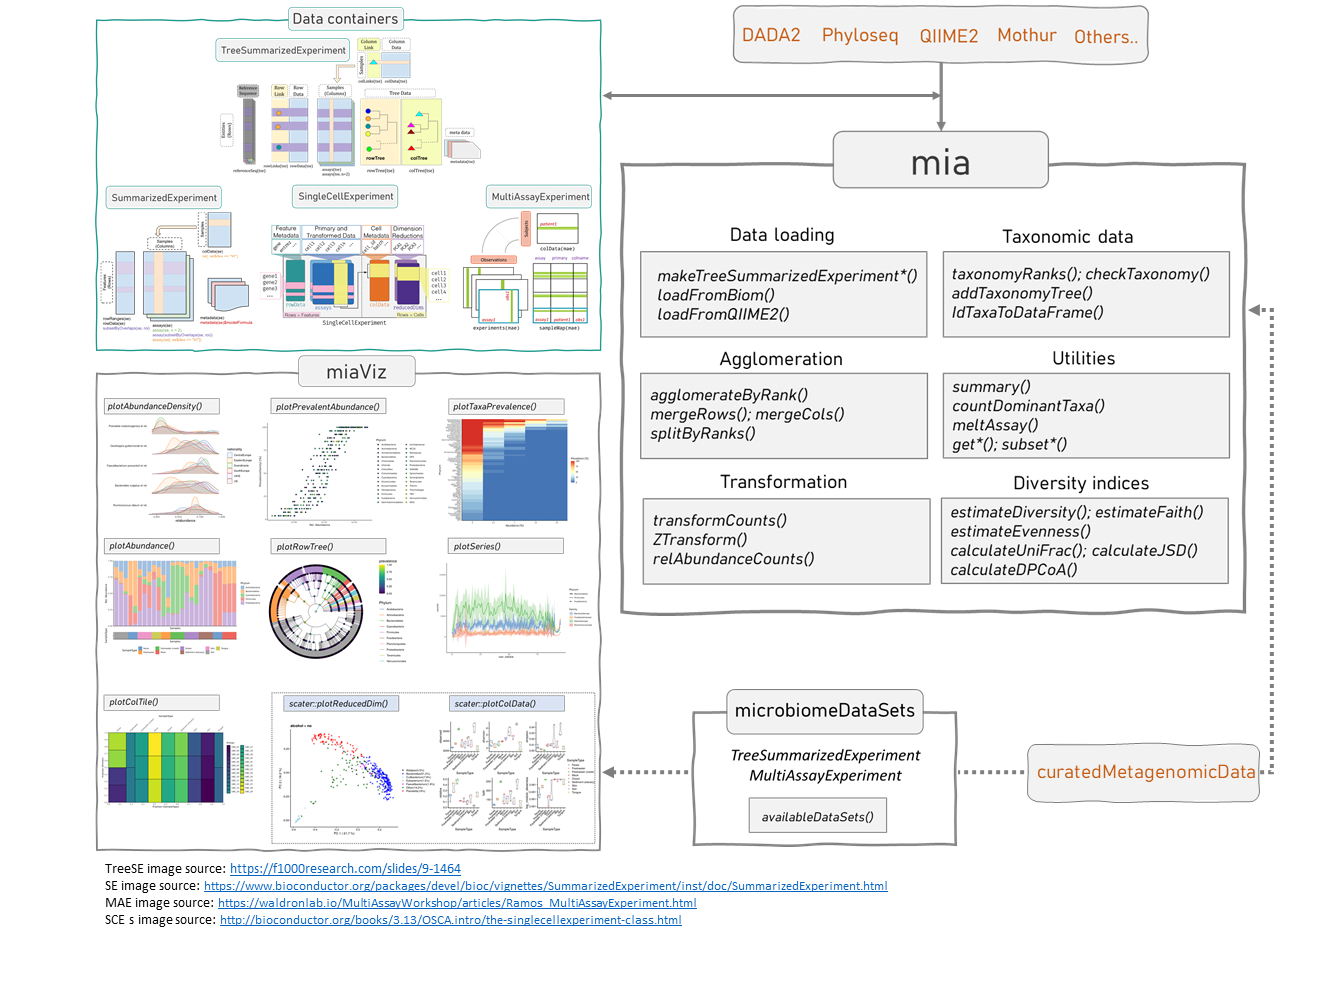
\includegraphics[width=18.67in]{general/figures/FigureOverviewV2}

\hypertarget{data-containers}{%
\section{Data containers}\label{data-containers}}

\href{https://bioconductor.org/packages/release/bioc/html/SummarizedExperiment.html}{\texttt{SummarizedExperiment}}
(\texttt{SE}) is a generic and highly optimized container for complex data
structures. It has become a common choice for analysing various types
of biomedical profiling data, such as RNAseq, ChIp-Seq, microarrays,
flow cytometry, proteomics, and single-cell
sequencing.

\href{https://www.bioconductor.org/packages/release/bioc/html/TreeSummarizedExperiment.html}{\texttt{TreeSummarizedExperiment}}
(\texttt{TreeSE}) was developed as an extension to incorporate hierarchical
information (such as phylogenetic trees and sample hierarchies) and
reference sequences.

\href{https://www.bioconductor.org/packages/release/bioc/html/MultiAssayExperiment.html}{\texttt{MultiAssayExperiment}}
(\texttt{MAE}) provides an organized way to bind several different data
structures together in a single object. For example, we can bind
microbiome data (in \texttt{TreeSE} format) with metabolomic profiling data
(in \texttt{SE}) format, with shared sample metadata. This is convenient and
robust for instance in subsetting and other data manipulation
tasks. Microbiome data can be part of multiomics experiments and
analysis strategies and we want to outline the understanding in which
we think the packages explained and used in this book relate to these
experiment layouts using the \texttt{TreeSummarizedExperiment} and classes
beyond.

This section provides an introductions to these data containers. In
microbiome data science, these containers link taxonomic abundance
tables with rich side information on the features and
samples. Taxonomic abundance data can be obtained by 16S rRNA amplicon
or metagenomic sequencing, phylogenetic microarrays, or by other
means. Many microbiome experiments include multiple versions and types
of data generated independently or derived from each other through
transformation or agglomeration. We start by providing recommendations
on how to represent different varieties of multi-table data within the
\texttt{TreeSummarizedExperiment} class.

The options and recommendations are summarized in Table \ref{tab:options}.

\hypertarget{assay-data}{%
\subsection{Assay data}\label{assay-data}}

The original count-based taxonomic abundance tables may have different
transformations, such as logarithmic, Centered Log-Ratio (CLR), or relative
abundance. These are typically stored in \emph{\textbf{assays}}.

\begin{Shaded}
\begin{Highlighting}[]
\FunctionTok{library}\NormalTok{(mia)}
\FunctionTok{data}\NormalTok{(GlobalPatterns, }\AttributeTok{package=}\StringTok{"mia"}\NormalTok{)}
\NormalTok{tse }\OtherTok{\textless{}{-}}\NormalTok{ GlobalPatterns}
\FunctionTok{assays}\NormalTok{(tse)}
\end{Highlighting}
\end{Shaded}

\begin{verbatim}
## List of length 1
## names(1): counts
\end{verbatim}

The \texttt{assays} slot contains the experimental data as count matrices. Multiple
matrices can be stored the result of \texttt{assays} is actually a list of matrices.

\begin{Shaded}
\begin{Highlighting}[]
\FunctionTok{assays}\NormalTok{(tse)}
\end{Highlighting}
\end{Shaded}

\begin{verbatim}
## List of length 1
## names(1): counts
\end{verbatim}

Individual assays can be accessed via \texttt{assay}

\begin{Shaded}
\begin{Highlighting}[]
\FunctionTok{assay}\NormalTok{(tse, }\StringTok{"counts"}\NormalTok{)[}\DecValTok{1}\SpecialCharTok{:}\DecValTok{5}\NormalTok{,}\DecValTok{1}\SpecialCharTok{:}\DecValTok{7}\NormalTok{]}
\end{Highlighting}
\end{Shaded}

\begin{verbatim}
##        CL3 CC1 SV1 M31Fcsw M11Fcsw M31Plmr M11Plmr
## 549322   0   0   0       0       0       0       0
## 522457   0   0   0       0       0       0       0
## 951      0   0   0       0       0       0       1
## 244423   0   0   0       0       0       0       0
## 586076   0   0   0       0       0       0       0
\end{verbatim}

To illustrate the use of multiple assays, the relative abundance data can be
calcualted and stored along the original count data using \texttt{relAbundanceCounts}.

\begin{Shaded}
\begin{Highlighting}[]
\NormalTok{tse }\OtherTok{\textless{}{-}} \FunctionTok{relAbundanceCounts}\NormalTok{(tse)}
\FunctionTok{assays}\NormalTok{(tse)}
\end{Highlighting}
\end{Shaded}

\begin{verbatim}
## List of length 2
## names(2): counts relabundance
\end{verbatim}

Now there are two assays available in the \texttt{tse} object, \texttt{counts} and
\texttt{relabundance}.

\begin{Shaded}
\begin{Highlighting}[]
\FunctionTok{assay}\NormalTok{(tse, }\StringTok{"relabundance"}\NormalTok{)[}\DecValTok{1}\SpecialCharTok{:}\DecValTok{5}\NormalTok{,}\DecValTok{1}\SpecialCharTok{:}\DecValTok{7}\NormalTok{]}
\end{Highlighting}
\end{Shaded}

\begin{verbatim}
##        CL3 CC1 SV1 M31Fcsw M11Fcsw M31Plmr   M11Plmr
## 549322   0   0   0       0       0       0 0.000e+00
## 522457   0   0   0       0       0       0 0.000e+00
## 951      0   0   0       0       0       0 2.305e-06
## 244423   0   0   0       0       0       0 0.000e+00
## 586076   0   0   0       0       0       0 0.000e+00
\end{verbatim}

Here the dimension of the count data remains unchanged. This is in
fact a requirement for any \texttt{SummarizedExperiment} object.

\hypertarget{coldata}{%
\subsection{colData}\label{coldata}}

\texttt{colData} contains data on the samples.

\begin{Shaded}
\begin{Highlighting}[]
\FunctionTok{colData}\NormalTok{(tse)}
\end{Highlighting}
\end{Shaded}

\begin{verbatim}
## DataFrame with 26 rows and 7 columns
##         X.SampleID   Primer Final_Barcode Barcode_truncated_plus_T
##           <factor> <factor>      <factor>                 <factor>
## CL3        CL3      ILBC_01        AACGCA                   TGCGTT
## CC1        CC1      ILBC_02        AACTCG                   CGAGTT
## SV1        SV1      ILBC_03        AACTGT                   ACAGTT
## M31Fcsw    M31Fcsw  ILBC_04        AAGAGA                   TCTCTT
## M11Fcsw    M11Fcsw  ILBC_05        AAGCTG                   CAGCTT
## ...            ...      ...           ...                      ...
## TS28         TS28   ILBC_25        ACCAGA                   TCTGGT
## TS29         TS29   ILBC_26        ACCAGC                   GCTGGT
## Even1        Even1  ILBC_27        ACCGCA                   TGCGGT
## Even2        Even2  ILBC_28        ACCTCG                   CGAGGT
## Even3        Even3  ILBC_29        ACCTGT                   ACAGGT
##         Barcode_full_length SampleType
##                    <factor>   <factor>
## CL3             CTAGCGTGCGT      Soil 
## CC1             CATCGACGAGT      Soil 
## SV1             GTACGCACAGT      Soil 
## M31Fcsw         TCGACATCTCT      Feces
## M11Fcsw         CGACTGCAGCT      Feces
## ...                     ...        ...
## TS28            GCATCGTCTGG      Feces
## TS29            CTAGTCGCTGG      Feces
## Even1           TGACTCTGCGG      Mock 
## Even2           TCTGATCGAGG      Mock 
## Even3           AGAGAGACAGG      Mock 
##                                        Description
##                                           <factor>
## CL3     Calhoun South Carolina Pine soil, pH 4.9  
## CC1     Cedar Creek Minnesota, grassland, pH 6.1  
## SV1     Sevilleta new Mexico, desert scrub, pH 8.3
## M31Fcsw M3, Day 1, fecal swab, whole body study   
## M11Fcsw M1, Day 1, fecal swab, whole body study   
## ...                                            ...
## TS28                                       Twin #1
## TS29                                       Twin #2
## Even1                                      Even1  
## Even2                                      Even2  
## Even3                                      Even3
\end{verbatim}

\hypertarget{rowdata}{%
\subsection{rowData}\label{rowdata}}

\texttt{rowData} contains data on the features of the analyzed samples. Of particular
interest for the microbiome field this is used to store taxonomic information.

\begin{Shaded}
\begin{Highlighting}[]
\FunctionTok{rowData}\NormalTok{(tse)}
\end{Highlighting}
\end{Shaded}

\begin{verbatim}
## DataFrame with 19216 rows and 7 columns
##            Kingdom        Phylum        Class        Order        Family
##        <character>   <character>  <character>  <character>   <character>
## 549322     Archaea Crenarchaeota Thermoprotei           NA            NA
## 522457     Archaea Crenarchaeota Thermoprotei           NA            NA
## 951        Archaea Crenarchaeota Thermoprotei Sulfolobales Sulfolobaceae
## 244423     Archaea Crenarchaeota        Sd-NA           NA            NA
## 586076     Archaea Crenarchaeota        Sd-NA           NA            NA
## ...            ...           ...          ...          ...           ...
## 278222    Bacteria           SR1           NA           NA            NA
## 463590    Bacteria           SR1           NA           NA            NA
## 535321    Bacteria           SR1           NA           NA            NA
## 200359    Bacteria           SR1           NA           NA            NA
## 271582    Bacteria           SR1           NA           NA            NA
##              Genus                Species
##        <character>            <character>
## 549322          NA                     NA
## 522457          NA                     NA
## 951     Sulfolobus Sulfolobusacidocalda..
## 244423          NA                     NA
## 586076          NA                     NA
## ...            ...                    ...
## 278222          NA                     NA
## 463590          NA                     NA
## 535321          NA                     NA
## 200359          NA                     NA
## 271582          NA                     NA
\end{verbatim}

\hypertarget{rowtree}{%
\subsection{rowTree}\label{rowtree}}

Phylogenetic trees also play an important role for the microbiome field. The
\texttt{TreeSummarizedExperiment} class is able to keep track of feature and node
relations via two functions, \texttt{rowTree} and \texttt{rowLinks}.

A tree can be accessed via \texttt{rowTree} as \texttt{phylo} object.

\begin{Shaded}
\begin{Highlighting}[]
\FunctionTok{rowTree}\NormalTok{(tse)}
\end{Highlighting}
\end{Shaded}

\begin{verbatim}
## 
## Phylogenetic tree with 19216 tips and 19215 internal nodes.
## 
## Tip labels:
##   549322, 522457, 951, 244423, 586076, 246140, ...
## Node labels:
##   , 0.858.4, 1.000.154, 0.764.3, 0.995.2, 1.000.2, ...
## 
## Rooted; includes branch lengths.
\end{verbatim}

The links to the individual features are available through \texttt{rowLinks}.

\begin{Shaded}
\begin{Highlighting}[]
\FunctionTok{rowLinks}\NormalTok{(tse)}
\end{Highlighting}
\end{Shaded}

\begin{verbatim}
## LinkDataFrame with 19216 rows and 5 columns
##           nodeLab   nodeNum nodeLab_alias    isLeaf   whichTree
##       <character> <integer>   <character> <logical> <character>
## 1          549322         1       alias_1      TRUE       phylo
## 2          522457         2       alias_2      TRUE       phylo
## 3             951         3       alias_3      TRUE       phylo
## 4          244423         4       alias_4      TRUE       phylo
## 5          586076         5       alias_5      TRUE       phylo
## ...           ...       ...           ...       ...         ...
## 19212      278222     19212   alias_19212      TRUE       phylo
## 19213      463590     19213   alias_19213      TRUE       phylo
## 19214      535321     19214   alias_19214      TRUE       phylo
## 19215      200359     19215   alias_19215      TRUE       phylo
## 19216      271582     19216   alias_19216      TRUE       phylo
\end{verbatim}

Please note that there can be a 1:1 relationship between tree nodes and
features, but this is not a must have. This means there can be features, which
are not linked to nodes, and nodes, which are not linked to features. To change
the links in an existing object, the \texttt{changeTree} function is available.

\hypertarget{alternative-experiments}{%
\subsection{Alternative experiments}\label{alternative-experiments}}

\emph{\textbf{Alternative experiments}} differ from transformations as they can
contain complementary data, which is no longer tied to the same
dimensions as the assay data. However, the number of samples (columns)
must be the same.

This can come into play for instance when one has taxonomic abundance
profiles quantified with different measurement technologies, such as
phylogenetic microarrays, amplicon sequencing, or metagenomic
sequencing. Such alternative experiments that concern the same samples
can be stored as

\begin{enumerate}
\def\labelenumi{\arabic{enumi}.}
\tightlist
\item
  Separate \emph{assays} assuming that the taxonomic information can be mapped
  between feature directly 1:1; or
\item
  data in the \emph{altExp} slot of the \texttt{TreeSummarizedExperiment}, if the feature
  dimensions differ. Each element of the \emph{altExp} slot is a \texttt{SummarizedExperiment}
  or an object from a derived class with independent feature data.
\end{enumerate}

As an example, we show how to store taxonomic abundance tables
agglomerated at different taxonomic levels. However, the data could as
well originate from entirely different measurement sources as long as
the samples are matched.

\begin{Shaded}
\begin{Highlighting}[]
\CommentTok{\# Agglomerate the data to Phylym level}
\NormalTok{tse\_phylum }\OtherTok{\textless{}{-}} \FunctionTok{agglomerateByRank}\NormalTok{(tse, }\StringTok{"Phylum"}\NormalTok{)}
\CommentTok{\# both have the same number of columns (samples)}
\FunctionTok{dim}\NormalTok{(tse)}
\end{Highlighting}
\end{Shaded}

\begin{verbatim}
## [1] 19216    26
\end{verbatim}

\begin{Shaded}
\begin{Highlighting}[]
\FunctionTok{dim}\NormalTok{(tse\_phylum)}
\end{Highlighting}
\end{Shaded}

\begin{verbatim}
## [1] 67 26
\end{verbatim}

\begin{Shaded}
\begin{Highlighting}[]
\CommentTok{\# Add the new table as an alternative experiment}
\FunctionTok{altExp}\NormalTok{(tse, }\StringTok{"Phylum"}\NormalTok{) }\OtherTok{\textless{}{-}}\NormalTok{ tse\_phylum}
\FunctionTok{altExpNames}\NormalTok{(tse)}
\end{Highlighting}
\end{Shaded}

\begin{verbatim}
## [1] "Phylum"
\end{verbatim}

\begin{Shaded}
\begin{Highlighting}[]
\CommentTok{\# Pick a sample subset: this acts on both altExp and assay data}
\NormalTok{tse[,}\DecValTok{1}\SpecialCharTok{:}\DecValTok{10}\NormalTok{]}
\end{Highlighting}
\end{Shaded}

\begin{verbatim}
## class: TreeSummarizedExperiment 
## dim: 19216 10 
## metadata(0):
## assays(2): counts relabundance
## rownames(19216): 549322 522457 ... 200359 271582
## rowData names(7): Kingdom Phylum ... Genus Species
## colnames(10): CL3 CC1 ... M31Tong M11Tong
## colData names(7): X.SampleID Primer ... SampleType Description
## reducedDimNames(0):
## mainExpName: NULL
## altExpNames(1): Phylum
## rowLinks: a LinkDataFrame (19216 rows)
## rowTree: 1 phylo tree(s) (19216 leaves)
## colLinks: NULL
## colTree: NULL
\end{verbatim}

\begin{Shaded}
\begin{Highlighting}[]
\FunctionTok{dim}\NormalTok{(}\FunctionTok{altExp}\NormalTok{(tse[,}\DecValTok{1}\SpecialCharTok{:}\DecValTok{10}\NormalTok{],}\StringTok{"Phylum"}\NormalTok{))}
\end{Highlighting}
\end{Shaded}

\begin{verbatim}
## [1] 67 10
\end{verbatim}

For more details of altExp have a look at the \href{https://bioconductor.org/packages/release/bioc/vignettes/SingleCellExperiment/inst/doc/intro.html}{Intro vignette} of the
\texttt{SingleCellExperiment} package \citep{R-SingleCellExperiment}.

\hypertarget{multiassayexperiments}{%
\subsection{MultiAssayExperiments}\label{multiassayexperiments}}

\emph{\textbf{Multiple experiments}} relate to complementary measurement types,
such as transcriptomic or metabolomic profiling of the microbiome or
the host. Multiple experiments can be represented using the same
options as alternative experiments, or by using the
\texttt{MultiAssayExperiment} class \citep{R-MultiAssayExperiment}. Depending on how the
datasets relate to each other the data can be stored as:

\begin{enumerate}
\def\labelenumi{\arabic{enumi}.}
\tightlist
\item
  Separate \emph{altExp} if the samples can be matched directly 1:1; or
\item
  As \texttt{MultiAssayExperiment} objects, in which the connections between
  samples are defined through a \texttt{sampleMap}. Each element on the
  \texttt{experimentsList} of an \texttt{MultiAssayExperiment} is \texttt{matrix} or
  \texttt{matrix}-like object including \texttt{SummarizedExperiment} objects, and the
  number of samples can differ between the elements.
\end{enumerate}

\begin{Shaded}
\begin{Highlighting}[]
\CommentTok{\#TODO: Find the right dataset to explain a non 1:1 sample relationship}
\end{Highlighting}
\end{Shaded}

For information have a look at the \href{https://bioconductor.org/packages/release/bioc/vignettes/MultiAssayExperiment/inst/doc/MultiAssayExperiment.html}{intro vignette} of the \texttt{MultiAssayExperiment} package.

\begin{longtable}[]{@{}rlrr@{}}
\caption{\label{tab:options} \textbf{Recommended options for storing multiple data tables in microbiome studies} The \emph{assays} are best suited for data transformations (one-to-one match between samples and columns across the assays). The \emph{alternative experiments} are particularly suitable for alternative versions of the data that are of same type but may have a different number of features (e.g.~taxonomic groups); this is for instance the case with taxonomic abundance tables agglomerated at different levels (e.g.~genus vs.~phyla) or alternative profiling technologies (e.g.~amplicon sequencing vs.~shallow shotgun metagenomics). For alternative experiments one-to-one match between samples (cols) is required but the alternative experiment tables can have different numbers of features (rows). Finally, elements of the \emph{MultiAssayExperiment} provide the most flexible way to incorporate multi-omic data tables with flexible numbers of samples and features. We recommend these conventions as the basis for methods development and application in microbiome studies.}\tabularnewline
\toprule
Option & Rows (features) & Cols (samples) & Recommended \\
\midrule
\endfirsthead
\toprule
Option & Rows (features) & Cols (samples) & Recommended \\
\midrule
\endhead
assays & match & match & Data transformations \\
altExp & free & match & Alternative experiments \\
MultiAssay & free & free (mapping) & Multi-omic experiments \\
\bottomrule
\end{longtable}

\hypertarget{loading-experimental-microbiome-data}{%
\section{Loading experimental microbiome data}\label{loading-experimental-microbiome-data}}

\hypertarget{import-from-external-files}{%
\subsection{Import from external files}\label{import-from-external-files}}

Microbiome (taxonomic) profiling data is commonly distributed in
various file formats. You can import such external data files as a
(Tree)SummarizedExperiment object but the details depend on the file
format. Here, we provide examples for common formats.

\textbf{CSV data tables} can be imported with the standard R functions,
then converted to the desired format. For detailed examples, you can
check the \href{https://bioconductor.org/help/course-materials/2019/BSS2019/04_Practical_CoreApproachesInBioconductor.html}{Bioconductor course
material}
by Martin Morgan. The following example reads abundance tables,
taxonomic mapping tables, and sample metadata, assuming that the
input data files are properly prepared with appropriate row and
column names.

\begin{Shaded}
\begin{Highlighting}[]
\NormalTok{counts  }\OtherTok{\textless{}{-}} \FunctionTok{read.csv}\NormalTok{(count\_file)   }\CommentTok{\# Abundance table (e.g. ASV data; to assay data)}
\NormalTok{tax     }\OtherTok{\textless{}{-}} \FunctionTok{read.csv}\NormalTok{(tax\_file)     }\CommentTok{\# Taxonomy table (to rowData)}
\NormalTok{samples }\OtherTok{\textless{}{-}} \FunctionTok{read.csv}\NormalTok{(sample\_file)  }\CommentTok{\# Sample data (to colData)}
\NormalTok{se }\OtherTok{\textless{}{-}} \FunctionTok{SummarizedExperiment}\NormalTok{(}\AttributeTok{assays =} \FunctionTok{list}\NormalTok{(}\AttributeTok{counts =}\NormalTok{ counts),}
                           \AttributeTok{colData =}\NormalTok{ samples,}
                           \AttributeTok{rowData =}\NormalTok{ tax)}
\end{Highlighting}
\end{Shaded}

Specific import functions are provided for:

\begin{itemize}
\tightlist
\item
  Biom files (see \texttt{help(mia::loadFromBiom)})
\item
  QIIME2 files (see \texttt{help(mia::loadFromQIIME2)})
\item
  Mothur files (see \texttt{help(mia::loadFromMothur)})
\end{itemize}

\hypertarget{biom-example}{%
\subsubsection{Biom example}\label{biom-example}}

This example shows how Biom files are imported into a
\texttt{TreeSummarizedExperiment} object.

The data is from following publication:
Tengeler AC \emph{et al.} (2020) \href{https://doi.org/10.1186/s40168-020-00816-x}{\textbf{Gut microbiota from persons with
attention-deficit/hyperactivity disorder affects the brain in
mice}}.

The data set consists of 3 files:

\begin{itemize}
\tightlist
\item
  biom file: abundance table and taxonomy information
\item
  csv file: sample metadata
\item
  tree file: phylogenetic tree
\end{itemize}

Store the data in your desired local directory (for instance, \emph{data/} under the
working directory), and define source file paths

\begin{Shaded}
\begin{Highlighting}[]
\NormalTok{biom\_file\_path }\OtherTok{\textless{}{-}} \StringTok{"data/Aggregated\_humanization2.biom"}
\NormalTok{sample\_meta\_file\_path }\OtherTok{\textless{}{-}} \StringTok{"data/Mapping\_file\_ADHD\_aggregated.csv"}
\NormalTok{tree\_file\_path }\OtherTok{\textless{}{-}} \StringTok{"data/Data\_humanization\_phylo\_aggregation.tre"}
\end{Highlighting}
\end{Shaded}

Now we can load the biom data into a SummarizedExperiment (SE) object.

\begin{Shaded}
\begin{Highlighting}[]
\FunctionTok{library}\NormalTok{(mia)}

\CommentTok{\# Imports the data}
\NormalTok{se }\OtherTok{\textless{}{-}} \FunctionTok{loadFromBiom}\NormalTok{(biom\_file\_path)}

\CommentTok{\# Check}
\NormalTok{se}
\end{Highlighting}
\end{Shaded}

\begin{verbatim}
## class: SummarizedExperiment 
## dim: 151 27 
## metadata(0):
## assays(1): counts
## rownames(151): 1726470 1726471 ... 17264756 17264757
## rowData names(6): taxonomy1 taxonomy2 ... taxonomy5 taxonomy6
## colnames(27): A110 A111 ... A38 A39
## colData names(0):
\end{verbatim}

The \texttt{assays} slot includes a list of abundance tables. The imported
abundance table is named as ``counts''. Let us inspect only the first
cols and rows.

\begin{Shaded}
\begin{Highlighting}[]
\FunctionTok{assays}\NormalTok{(se)}\SpecialCharTok{$}\NormalTok{counts[}\DecValTok{1}\SpecialCharTok{:}\DecValTok{3}\NormalTok{, }\DecValTok{1}\SpecialCharTok{:}\DecValTok{3}\NormalTok{]}
\end{Highlighting}
\end{Shaded}

\begin{verbatim}
##           A110  A111  A12
## 1726470  17722 11630    0
## 1726471  12052     0 2679
## 17264731     0   970    0
\end{verbatim}

The \texttt{rowdata} includes taxonomic information from the biom file. The \texttt{head()} command
shows just the beginning of the data table for an overview.

\texttt{knitr::kable()} is for printing the information more nicely.

\begin{Shaded}
\begin{Highlighting}[]
\FunctionTok{head}\NormalTok{(}\FunctionTok{rowData}\NormalTok{(se))}
\end{Highlighting}
\end{Shaded}

\begin{verbatim}
## DataFrame with 6 rows and 6 columns
##             taxonomy1          taxonomy2           taxonomy3
##           <character>        <character>         <character>
## 1726470  "k__Bacteria   p__Bacteroidetes      c__Bacteroidia
## 1726471  "k__Bacteria   p__Bacteroidetes      c__Bacteroidia
## 17264731 "k__Bacteria   p__Bacteroidetes      c__Bacteroidia
## 17264726 "k__Bacteria   p__Bacteroidetes      c__Bacteroidia
## 1726472  "k__Bacteria p__Verrucomicrobia c__Verrucomicrobiae
## 17264724 "k__Bacteria   p__Bacteroidetes      c__Bacteroidia
##                      taxonomy4              taxonomy5           taxonomy6
##                    <character>            <character>         <character>
## 1726470       o__Bacteroidales      f__Bacteroidaceae     g__Bacteroides"
## 1726471       o__Bacteroidales      f__Bacteroidaceae     g__Bacteroides"
## 17264731      o__Bacteroidales  f__Porphyromonadaceae g__Parabacteroides"
## 17264726      o__Bacteroidales      f__Bacteroidaceae     g__Bacteroides"
## 1726472  o__Verrucomicrobiales f__Verrucomicrobiaceae     g__Akkermansia"
## 17264724      o__Bacteroidales      f__Bacteroidaceae     g__Bacteroides"
\end{verbatim}

These taxonomic rank names (column names) are not real rank
names. Let's replace them with real rank names.

In addition to that, the taxa names include, e.g., '\,``k\_\_' before the name, so let's
make them cleaner by removing them.

\begin{Shaded}
\begin{Highlighting}[]
\FunctionTok{names}\NormalTok{(}\FunctionTok{rowData}\NormalTok{(se)) }\OtherTok{\textless{}{-}} \FunctionTok{c}\NormalTok{(}\StringTok{"Kingdom"}\NormalTok{, }\StringTok{"Phylum"}\NormalTok{, }\StringTok{"Class"}\NormalTok{, }\StringTok{"Order"}\NormalTok{, }
                        \StringTok{"Family"}\NormalTok{, }\StringTok{"Genus"}\NormalTok{)}

\CommentTok{\# Goes through the whole DataFrame. Removes \textquotesingle{}.*[kpcofg]\_\_\textquotesingle{} from strings, where [kpcofg] }
\CommentTok{\# is any character from listed ones, and .* any character.}
\NormalTok{rowdata\_modified }\OtherTok{\textless{}{-}}\NormalTok{ BiocParallel}\SpecialCharTok{::}\FunctionTok{bplapply}\NormalTok{(}\FunctionTok{rowData}\NormalTok{(se), }
                                           \AttributeTok{FUN =}\NormalTok{ stringr}\SpecialCharTok{::}\NormalTok{str\_remove, }
                                           \AttributeTok{pattern =} \StringTok{\textquotesingle{}.*[kpcofg]\_\_\textquotesingle{}}\NormalTok{)}

\CommentTok{\# Genus level has additional \textquotesingle{}\textbackslash{}"\textquotesingle{}, so let\textquotesingle{}s delete that also}
\NormalTok{rowdata\_modified }\OtherTok{\textless{}{-}}\NormalTok{ BiocParallel}\SpecialCharTok{::}\FunctionTok{bplapply}\NormalTok{(rowdata\_modified, }
                                           \AttributeTok{FUN =}\NormalTok{ stringr}\SpecialCharTok{::}\NormalTok{str\_remove, }
                                           \AttributeTok{pattern =} \StringTok{\textquotesingle{}}\SpecialCharTok{\textbackslash{}"}\StringTok{\textquotesingle{}}\NormalTok{)}

\CommentTok{\# rowdata\_modified is a list, so it is converted back to DataFrame format. }
\NormalTok{rowdata\_modified }\OtherTok{\textless{}{-}} \FunctionTok{DataFrame}\NormalTok{(rowdata\_modified)}

\CommentTok{\# And then assigned back to the SE object}
\FunctionTok{rowData}\NormalTok{(se) }\OtherTok{\textless{}{-}}\NormalTok{ rowdata\_modified}

\CommentTok{\# Now we have a nicer table}
\FunctionTok{head}\NormalTok{(}\FunctionTok{rowData}\NormalTok{(se))}
\end{Highlighting}
\end{Shaded}

\begin{verbatim}
## DataFrame with 6 rows and 6 columns
##              Kingdom          Phylum            Class              Order
##          <character>     <character>      <character>        <character>
## 1726470     Bacteria   Bacteroidetes      Bacteroidia      Bacteroidales
## 1726471     Bacteria   Bacteroidetes      Bacteroidia      Bacteroidales
## 17264731    Bacteria   Bacteroidetes      Bacteroidia      Bacteroidales
## 17264726    Bacteria   Bacteroidetes      Bacteroidia      Bacteroidales
## 1726472     Bacteria Verrucomicrobia Verrucomicrobiae Verrucomicrobiales
## 17264724    Bacteria   Bacteroidetes      Bacteroidia      Bacteroidales
##                       Family           Genus
##                  <character>     <character>
## 1726470       Bacteroidaceae     Bacteroides
## 1726471       Bacteroidaceae     Bacteroides
## 17264731  Porphyromonadaceae Parabacteroides
## 17264726      Bacteroidaceae     Bacteroides
## 1726472  Verrucomicrobiaceae     Akkermansia
## 17264724      Bacteroidaceae     Bacteroides
\end{verbatim}

We notice that the imported biom file did not contain the sample meta data
yet, so it includes an empty data frame.

\begin{Shaded}
\begin{Highlighting}[]
\FunctionTok{head}\NormalTok{(}\FunctionTok{colData}\NormalTok{(se))}
\end{Highlighting}
\end{Shaded}

\begin{verbatim}
## DataFrame with 6 rows and 0 columns
\end{verbatim}

Let us add a sample metadata file.

\begin{Shaded}
\begin{Highlighting}[]
\CommentTok{\# We use this to check what type of data it is}
\CommentTok{\# read.table(sample\_meta\_file\_path)}

\CommentTok{\# It seems like a comma separated file and it does not include headers}
\CommentTok{\# Let us read it and then convert from data.frame to DataFrame}
\CommentTok{\# (required for our purposes)}
\NormalTok{sample\_meta }\OtherTok{\textless{}{-}} \FunctionTok{DataFrame}\NormalTok{(}\FunctionTok{read.table}\NormalTok{(sample\_meta\_file\_path, }\AttributeTok{sep =} \StringTok{","}\NormalTok{, }\AttributeTok{header =} \ConstantTok{FALSE}\NormalTok{))}

\CommentTok{\# Add sample names to rownames}
\FunctionTok{rownames}\NormalTok{(sample\_meta) }\OtherTok{\textless{}{-}}\NormalTok{ sample\_meta[,}\DecValTok{1}\NormalTok{]}

\CommentTok{\# Delete column that included sample names}
\NormalTok{sample\_meta[,}\DecValTok{1}\NormalTok{] }\OtherTok{\textless{}{-}} \ConstantTok{NULL}

\CommentTok{\# We can add headers}
\FunctionTok{colnames}\NormalTok{(sample\_meta) }\OtherTok{\textless{}{-}} \FunctionTok{c}\NormalTok{(}\StringTok{"patient\_status"}\NormalTok{, }\StringTok{"cohort"}\NormalTok{, }\StringTok{"patient\_status\_vs\_cohort"}\NormalTok{, }\StringTok{"sample\_name"}\NormalTok{)}

\CommentTok{\# Then it can be added to colData}
\FunctionTok{colData}\NormalTok{(se) }\OtherTok{\textless{}{-}}\NormalTok{ sample\_meta}
\end{Highlighting}
\end{Shaded}

Now \texttt{colData} includes the sample metadata.

\begin{Shaded}
\begin{Highlighting}[]
\FunctionTok{head}\NormalTok{(}\FunctionTok{colData}\NormalTok{(se))}
\end{Highlighting}
\end{Shaded}

\begin{verbatim}
## DataFrame with 6 rows and 4 columns
##      patient_status      cohort patient_status_vs_cohort sample_name
##         <character> <character>              <character> <character>
## A110           ADHD    Cohort_1            ADHD_Cohort_1        A110
## A12            ADHD    Cohort_1            ADHD_Cohort_1         A12
## A15            ADHD    Cohort_1            ADHD_Cohort_1         A15
## A19            ADHD    Cohort_1            ADHD_Cohort_1         A19
## A21            ADHD    Cohort_2            ADHD_Cohort_2         A21
## A23            ADHD    Cohort_2            ADHD_Cohort_2         A23
\end{verbatim}

Now, let's add a phylogenetic tree.

The current data object, se, is a SummarizedExperiment object. This
does not include a slot for adding a phylogenetic tree. In order to do
this, we can convert the SE object to an extended TreeSummarizedExperiment
object which includes also a \texttt{rowTree} slot.

\begin{Shaded}
\begin{Highlighting}[]
\NormalTok{tse }\OtherTok{\textless{}{-}} \FunctionTok{as}\NormalTok{(se, }\StringTok{"TreeSummarizedExperiment"}\NormalTok{)}

\CommentTok{\# tse includes same data as se}
\NormalTok{tse}
\end{Highlighting}
\end{Shaded}

\begin{verbatim}
## class: TreeSummarizedExperiment 
## dim: 151 27 
## metadata(0):
## assays(1): counts
## rownames(151): 1726470 1726471 ... 17264756 17264757
## rowData names(6): Kingdom Phylum ... Family Genus
## colnames(27): A110 A12 ... A35 A38
## colData names(4): patient_status cohort patient_status_vs_cohort
##   sample_name
## reducedDimNames(0):
## mainExpName: NULL
## altExpNames(0):
## rowLinks: NULL
## rowTree: NULL
## colLinks: NULL
## colTree: NULL
\end{verbatim}

Next, let us read the tree data file and add it to the R data object (tse).

\begin{Shaded}
\begin{Highlighting}[]
\CommentTok{\# Reads the tree file}
\NormalTok{tree }\OtherTok{\textless{}{-}}\NormalTok{ ape}\SpecialCharTok{::}\FunctionTok{read.tree}\NormalTok{(tree\_file\_path)}

\CommentTok{\# Add tree to rowTree}
\FunctionTok{rowTree}\NormalTok{(tse) }\OtherTok{\textless{}{-}}\NormalTok{ tree}

\CommentTok{\# Check}
\NormalTok{tse}
\end{Highlighting}
\end{Shaded}

\begin{verbatim}
## class: TreeSummarizedExperiment 
## dim: 151 27 
## metadata(0):
## assays(1): counts
## rownames(151): 1726470 1726471 ... 17264756 17264757
## rowData names(6): Kingdom Phylum ... Family Genus
## colnames(27): A110 A12 ... A35 A38
## colData names(4): patient_status cohort patient_status_vs_cohort
##   sample_name
## reducedDimNames(0):
## mainExpName: NULL
## altExpNames(0):
## rowLinks: a LinkDataFrame (151 rows)
## rowTree: 1 phylo tree(s) (151 leaves)
## colLinks: NULL
## colTree: NULL
\end{verbatim}

Now \texttt{rowTree} includes a phylogenetic tree:

\begin{Shaded}
\begin{Highlighting}[]
\FunctionTok{head}\NormalTok{(}\FunctionTok{rowTree}\NormalTok{(tse))}
\end{Highlighting}
\end{Shaded}

\hypertarget{conversions-between-data-formats-in-r}{%
\subsection{Conversions between data formats in R}\label{conversions-between-data-formats-in-r}}

If the data has already been imported in R in another format, it
can be readily converted into \texttt{TreeSummarizedExperiment}, as shown in our next
example. Note that similar conversion functions to
\texttt{TreeSummarizedExperiment} are available for multiple data formats via
the \texttt{mia} package (see makeTreeSummarizedExperimentFrom* for phyloseq,
Biom, and DADA2).

\begin{Shaded}
\begin{Highlighting}[]
\FunctionTok{library}\NormalTok{(mia)}

\CommentTok{\# phyloseq example data}
\FunctionTok{data}\NormalTok{(GlobalPatterns, }\AttributeTok{package=}\StringTok{"phyloseq"}\NormalTok{) }
\NormalTok{GlobalPatterns\_phyloseq }\OtherTok{\textless{}{-}}\NormalTok{ GlobalPatterns}
\NormalTok{GlobalPatterns\_phyloseq}
\end{Highlighting}
\end{Shaded}

\begin{verbatim}
## phyloseq-class experiment-level object
## otu_table()   OTU Table:         [ 19216 taxa and 26 samples ]
## sample_data() Sample Data:       [ 26 samples by 7 sample variables ]
## tax_table()   Taxonomy Table:    [ 19216 taxa by 7 taxonomic ranks ]
## phy_tree()    Phylogenetic Tree: [ 19216 tips and 19215 internal nodes ]
\end{verbatim}

\begin{Shaded}
\begin{Highlighting}[]
\CommentTok{\# convert phyloseq to TSE}
\NormalTok{GlobalPatterns\_TSE }\OtherTok{\textless{}{-}} \FunctionTok{makeTreeSummarizedExperimentFromPhyloseq}\NormalTok{(GlobalPatterns\_phyloseq) }
\NormalTok{GlobalPatterns\_TSE}
\end{Highlighting}
\end{Shaded}

\begin{verbatim}
## class: TreeSummarizedExperiment 
## dim: 19216 26 
## metadata(0):
## assays(1): counts
## rownames(19216): 549322 522457 ... 200359 271582
## rowData names(7): Kingdom Phylum ... Genus Species
## colnames(26): CL3 CC1 ... Even2 Even3
## colData names(7): X.SampleID Primer ... SampleType Description
## reducedDimNames(0):
## mainExpName: NULL
## altExpNames(0):
## rowLinks: a LinkDataFrame (19216 rows)
## rowTree: 1 phylo tree(s) (19216 leaves)
## colLinks: NULL
## colTree: NULL
\end{verbatim}

We can also convert \texttt{TreeSummarizedExperiment} objects into \texttt{phyloseq}
with respect to the shared components that are supported by both
formats (i.e.~taxonomic abundance table, sample metadata, taxonomic
table, phylogenetic tree, sequence information). This is useful for
instance when additional methods are available for \texttt{phyloseq}.

\begin{Shaded}
\begin{Highlighting}[]
\CommentTok{\# convert TSE to phyloseq}
\NormalTok{GlobalPatterns\_phyloseq2 }\OtherTok{\textless{}{-}} \FunctionTok{makePhyloseqFromTreeSummarizedExperiment}\NormalTok{(GlobalPatterns\_TSE) }
\NormalTok{GlobalPatterns\_phyloseq2}
\end{Highlighting}
\end{Shaded}

\begin{verbatim}
## phyloseq-class experiment-level object
## otu_table()   OTU Table:         [ 19216 taxa and 26 samples ]
## sample_data() Sample Data:       [ 26 samples by 7 sample variables ]
## tax_table()   Taxonomy Table:    [ 19216 taxa by 7 taxonomic ranks ]
## phy_tree()    Phylogenetic Tree: [ 19216 tips and 19215 internal nodes ]
\end{verbatim}

Conversion is possible between other data formats. Interested readers can refer to the following functions:
* \href{https://microbiome.github.io/mia/reference/makeTreeSummarizedExperimentFromDADA2.html}{makeTreeSummarizedExperimentFromDADA2}
* \href{https://microbiome.github.io/mia/reference/makeSummarizedExperimentFromBiom.html}{makeSummarizedExperimentFromBiom}
* \href{https://microbiome.github.io/mia/reference/loadFromMetaphlan.html}{loadFromMetaphlan}
* \href{https://microbiome.github.io/mia/reference/loadFromQIIME2.html}{readQZA}

\hypertarget{example-data}{%
\section{Demonstration data}\label{example-data}}

Open demonstration data for testing and benchmarking purposes is
available from multiple locations. This chapter introduces some
options. The other chapters of this book provide ample examples about
the use of the data.

\hypertarget{package-data}{%
\subsection{Package data}\label{package-data}}

The \texttt{mia} R package contains example data sets that are direct
conversions from the alternative \texttt{phyloseq} container to the
\texttt{TreeSummarizedExperiment} container.

List the \href{https://microbiome.github.io/mia/reference/index.html}{available
datasets} in
the \texttt{mia} package:

\begin{Shaded}
\begin{Highlighting}[]
\FunctionTok{library}\NormalTok{(mia)}
\FunctionTok{data}\NormalTok{(}\AttributeTok{package=}\StringTok{"mia"}\NormalTok{)}
\end{Highlighting}
\end{Shaded}

Load the \texttt{GlobalPatterns} data from the \texttt{mia} package:

\begin{Shaded}
\begin{Highlighting}[]
\FunctionTok{data}\NormalTok{(}\StringTok{"GlobalPatterns"}\NormalTok{, }\AttributeTok{package=}\StringTok{"mia"}\NormalTok{)}
\NormalTok{GlobalPatterns}
\end{Highlighting}
\end{Shaded}

\begin{verbatim}
## class: TreeSummarizedExperiment 
## dim: 19216 26 
## metadata(0):
## assays(1): counts
## rownames(19216): 549322 522457 ... 200359 271582
## rowData names(7): Kingdom Phylum ... Genus Species
## colnames(26): CL3 CC1 ... Even2 Even3
## colData names(7): X.SampleID Primer ... SampleType Description
## reducedDimNames(0):
## mainExpName: NULL
## altExpNames(0):
## rowLinks: a LinkDataFrame (19216 rows)
## rowTree: 1 phylo tree(s) (19216 leaves)
## colLinks: NULL
## colTree: NULL
\end{verbatim}

Check the documentation for this data set:

\begin{verbatim}
## Help on topic 'GlobalPatterns' was found in the following packages:
## 
##   Package               Library
##   phyloseq              /__w/_temp/Library
##   mia                   /__w/_temp/Library
## 
## 
## Using the first match ...
\end{verbatim}

\hypertarget{experimenthub-data}{%
\subsection{ExperimentHub data}\label{experimenthub-data}}

\href{https://bioconductor.org/packages/release/bioc/vignettes/ExperimentHub/inst/doc/ExperimentHub.html}{ExperimentHub}
provides a variety of data resources, including the
\href{https://bioconductor.org/packages/devel/data/experiment/html/microbiomeDataSets.html}{microbiomeDataSets}
package.

A table of the available data sets is available through the \texttt{availableDataSets}
function.

\begin{Shaded}
\begin{Highlighting}[]
\FunctionTok{library}\NormalTok{(microbiomeDataSets)}
\FunctionTok{availableDataSets}\NormalTok{()}
\end{Highlighting}
\end{Shaded}

\begin{verbatim}
##             Dataset
## 1  GrieneisenTSData
## 2    HintikkaXOData
## 3       LahtiMLData
## 4        LahtiMData
## 5       LahtiWAData
## 6      OKeefeDSData
## 7 SilvermanAGutData
## 8        SongQAData
## 9   SprockettTHData
\end{verbatim}

All data are downloaded from ExperimentHub and cached for local
re-use. Check the \href{https://microbiome.github.io/microbiomeDataSets/reference/index.html}{man pages of each
function}
for a detailed documentation of the data contents and references. Let
us retrieve a \emph{\href{https://bioconductor.org/packages/3.14/MultiAssayExperiment}{MultiAssayExperiment}} data set:

\begin{Shaded}
\begin{Highlighting}[]
\NormalTok{mae }\OtherTok{\textless{}{-}} \FunctionTok{HintikkaXOData}\NormalTok{()}
\end{Highlighting}
\end{Shaded}

Data is available in \emph{\href{https://bioconductor.org/packages/3.14/SummarizedExperiment}{SummarizedExperiment}}, \texttt{r\ Biocpkg("TreeSummarizedExperiment")}, and \texttt{r\ Biocpkg("MultiAssayExperiment")} data containers; see the separate
page on \href{https://microbiome.github.io/OMA/multitable.html}{alternative
containers} for more
details.

\hypertarget{other-data-sources}{%
\subsection{Other data sources}\label{other-data-sources}}

The
\href{https://waldronlab.io/curatedMetagenomicData}{curatedMetagenomicData}
is an independent source that provides various example data sets as
\texttt{(Tree)SummarizedExperiment} objects. This resource provides curated
human microbiome data including gene families, marker abundance,
marker presence, pathway abundance, pathway coverage, and relative
abundance for samples from different body sites. See the package
homepage for more details on data availability and access.

As one example, let us retrieve the Vatanen (2016) \citep{Vatanen2016} data
set. This is a larger collection with a bit longer download time.

\begin{Shaded}
\begin{Highlighting}[]
\FunctionTok{library}\NormalTok{(curatedMetagenomicData)}
\NormalTok{tse }\OtherTok{\textless{}{-}} \FunctionTok{curatedMetagenomicData}\NormalTok{(}\StringTok{"Vatanen*"}\NormalTok{, }\AttributeTok{dryrun =} \ConstantTok{FALSE}\NormalTok{, }\AttributeTok{counts =} \ConstantTok{TRUE}\NormalTok{)}
\end{Highlighting}
\end{Shaded}

\hypertarget{session-info}{%
\section*{Session Info}\label{session-info}}
\addcontentsline{toc}{section}{Session Info}

View session info

\begin{verbatim}
R version 4.1.2 (2021-11-01)
Platform: x86_64-pc-linux-gnu (64-bit)
Running under: Ubuntu 20.04.3 LTS

Matrix products: default
BLAS/LAPACK: /usr/lib/x86_64-linux-gnu/openblas-pthread/libopenblasp-r0.3.8.so

locale:
 [1] LC_CTYPE=en_US.UTF-8       LC_NUMERIC=C              
 [3] LC_TIME=en_US.UTF-8        LC_COLLATE=en_US.UTF-8    
 [5] LC_MONETARY=en_US.UTF-8    LC_MESSAGES=en_US.UTF-8   
 [7] LC_PAPER=en_US.UTF-8       LC_NAME=C                 
 [9] LC_ADDRESS=C               LC_TELEPHONE=C            
[11] LC_MEASUREMENT=en_US.UTF-8 LC_IDENTIFICATION=C       

attached base packages:
[1] stats4    stats     graphics  grDevices utils     datasets  methods  
[8] base     

other attached packages:
 [1] microbiomeDataSets_1.1.5       phyloseq_1.38.0               
 [3] mia_1.3.19                     MultiAssayExperiment_1.20.0   
 [5] TreeSummarizedExperiment_2.1.4 Biostrings_2.62.0             
 [7] XVector_0.34.0                 SingleCellExperiment_1.16.0   
 [9] SummarizedExperiment_1.24.0    Biobase_2.54.0                
[11] GenomicRanges_1.46.1           GenomeInfoDb_1.30.1           
[13] IRanges_2.28.0                 S4Vectors_0.32.3              
[15] BiocGenerics_0.40.0            MatrixGenerics_1.6.0          
[17] matrixStats_0.61.0-9001        BiocStyle_2.22.0              
[19] rebook_1.4.0                  

loaded via a namespace (and not attached):
  [1] AnnotationHub_3.2.2           BiocFileCache_2.2.1          
  [3] plyr_1.8.6                    igraph_1.2.11                
  [5] lazyeval_0.2.2                splines_4.1.2                
  [7] BiocParallel_1.28.3           ggplot2_3.3.5                
  [9] scater_1.22.0                 digest_0.6.29                
 [11] foreach_1.5.2                 yulab.utils_0.0.4            
 [13] htmltools_0.5.2               viridis_0.6.2                
 [15] fansi_1.0.2                   magrittr_2.0.2               
 [17] memoise_2.0.1                 ScaledMatrix_1.2.0           
 [19] cluster_2.1.2                 DECIPHER_2.22.0              
 [21] colorspace_2.0-3              blob_1.2.2                   
 [23] rappdirs_0.3.3                ggrepel_0.9.1                
 [25] xfun_0.30                     dplyr_1.0.8                  
 [27] crayon_1.5.0                  RCurl_1.98-1.6               
 [29] jsonlite_1.8.0                graph_1.72.0                 
 [31] survival_3.3-1                iterators_1.0.14             
 [33] ape_5.6-2                     glue_1.6.2                   
 [35] gtable_0.3.0                  zlibbioc_1.40.0              
 [37] DelayedArray_0.20.0           BiocSingular_1.10.0          
 [39] Rhdf5lib_1.16.0               scales_1.1.1                 
 [41] DBI_1.1.2                     Rcpp_1.0.8.3                 
 [43] xtable_1.8-4                  viridisLite_0.4.0            
 [45] decontam_1.14.0               tidytree_0.3.9               
 [47] bit_4.0.4                     rsvd_1.0.5                   
 [49] httr_1.4.2                    dir.expiry_1.2.0             
 [51] ellipsis_0.3.2                pkgconfig_2.0.3              
 [53] XML_3.99-0.9                  scuttle_1.4.0                
 [55] CodeDepends_0.6.5             dbplyr_2.1.1                 
 [57] utf8_1.2.2                    AnnotationDbi_1.56.2         
 [59] later_1.3.0                   tidyselect_1.1.2             
 [61] rlang_1.0.2                   reshape2_1.4.4               
 [63] munsell_0.5.0                 BiocVersion_3.14.0           
 [65] tools_4.1.2                   cachem_1.0.6                 
 [67] cli_3.2.0                     DirichletMultinomial_1.36.0  
 [69] generics_0.1.2                RSQLite_2.2.10               
 [71] ExperimentHub_2.2.1           ade4_1.7-18                  
 [73] evaluate_0.15                 biomformat_1.22.0            
 [75] stringr_1.4.0                 fastmap_1.1.0                
 [77] yaml_2.3.5                    knitr_1.37                   
 [79] bit64_4.0.5                   purrr_0.3.4                  
 [81] KEGGREST_1.34.0               nlme_3.1-155                 
 [83] sparseMatrixStats_1.6.0       mime_0.12                    
 [85] compiler_4.1.2                interactiveDisplayBase_1.32.0
 [87] beeswarm_0.4.0                filelock_1.0.2               
 [89] curl_4.3.2                    png_0.1-7                    
 [91] treeio_1.18.1                 tibble_3.1.6                 
 [93] stringi_1.7.6                 lattice_0.20-45              
 [95] Matrix_1.4-0                  vegan_2.5-7                  
 [97] permute_0.9-7                 multtest_2.50.0              
 [99] vctrs_0.3.8                   pillar_1.7.0                 
[101] lifecycle_1.0.1               rhdf5filters_1.6.0           
[103] BiocManager_1.30.16           BiocNeighbors_1.12.0         
[105] data.table_1.14.2             bitops_1.0-7                 
[107] irlba_2.3.5                   httpuv_1.6.5                 
[109] R6_2.5.1                      promises_1.2.0.1             
[111] bookdown_0.25                 gridExtra_2.3                
[113] vipor_0.4.5                   codetools_0.2-18             
[115] MASS_7.3-55                   assertthat_0.2.1             
[117] rhdf5_2.38.1                  GenomeInfoDbData_1.2.7       
[119] mgcv_1.8-39                   parallel_4.1.2               
[121] grid_4.1.2                    beachmat_2.10.0              
[123] tidyr_1.2.0                   rmarkdown_2.13               
[125] DelayedMatrixStats_1.16.0     shiny_1.7.1                  
[127] ggbeeswarm_0.6.0             
\end{verbatim}

\hypertarget{packages}{%
\chapter{Packages}\label{packages}}

\hypertarget{package-installation}{%
\section{Package installation}\label{package-installation}}

Several R packages provide methods for the analysis and manipulation
of \texttt{SummarizedExperiment} and related data containers. One of these is
\texttt{mia}. The installation for this and other packages has the following
procedure.

Stable Biocondcuctor release version can be installed with:

\begin{Shaded}
\begin{Highlighting}[]
\NormalTok{BiocManager}\SpecialCharTok{::}\FunctionTok{install}\NormalTok{(}\StringTok{"microbiome/mia"}\NormalTok{)}
\end{Highlighting}
\end{Shaded}

Biocondcuctor development version requires the installation of the
latest R beta version, and this is primarily recommended for those who
already have solid experience with R/Bioconductor and need access to
the latest experimental updates.

\begin{Shaded}
\begin{Highlighting}[]
\NormalTok{BiocManager}\SpecialCharTok{::}\FunctionTok{install}\NormalTok{(}\StringTok{"microbiome/mia"}\NormalTok{, }\AttributeTok{version=}\StringTok{"devel"}\NormalTok{)}
\end{Highlighting}
\end{Shaded}

The bleeding edge (and potentially unstable) development version lives
in Github:

\begin{Shaded}
\begin{Highlighting}[]
\NormalTok{devtools}\SpecialCharTok{::}\FunctionTok{install\_github}\NormalTok{(}\StringTok{"microbiome/mia"}\NormalTok{)}
\end{Highlighting}
\end{Shaded}

\hypertarget{some-available-packages}{%
\section{Some available packages}\label{some-available-packages}}

Some of the R packages supporting the framework include:

\begin{itemize}
\tightlist
\item
  \href{microbiome.github.io/mia}{mia} : Microbiome analysis tools\\
\item
  \href{microbiome.github.io/miaViz}{miaViz} : Microbiome analysis specific visualization
\item
  \href{microbiome.github.io/miaSim}{miaSim} : Microbiome data simulations
\item
  \href{microbiome.github.io/miaTime}{miaTime} : Microbiome time series analysis
\item
  \href{http://bioconductor.org/packages/devel/bioc/html/philr.html}{philr} (external)
\end{itemize}

\hypertarget{session-info-1}{%
\section*{Session Info}\label{session-info-1}}
\addcontentsline{toc}{section}{Session Info}

View session info

\begin{verbatim}
R version 4.1.2 (2021-11-01)
Platform: x86_64-pc-linux-gnu (64-bit)
Running under: Ubuntu 20.04.3 LTS

Matrix products: default
BLAS/LAPACK: /usr/lib/x86_64-linux-gnu/openblas-pthread/libopenblasp-r0.3.8.so

locale:
 [1] LC_CTYPE=en_US.UTF-8       LC_NUMERIC=C              
 [3] LC_TIME=en_US.UTF-8        LC_COLLATE=en_US.UTF-8    
 [5] LC_MONETARY=en_US.UTF-8    LC_MESSAGES=en_US.UTF-8   
 [7] LC_PAPER=en_US.UTF-8       LC_NAME=C                 
 [9] LC_ADDRESS=C               LC_TELEPHONE=C            
[11] LC_MEASUREMENT=en_US.UTF-8 LC_IDENTIFICATION=C       

attached base packages:
[1] stats     graphics  grDevices utils     datasets  methods   base     

other attached packages:
[1] BiocStyle_2.22.0 rebook_1.4.0    

loaded via a namespace (and not attached):
 [1] bookdown_0.25       dir.expiry_1.2.0    codetools_0.2-18   
 [4] XML_3.99-0.9        digest_0.6.29       stats4_4.1.2       
 [7] magrittr_2.0.2      evaluate_0.15       graph_1.72.0       
[10] rlang_1.0.2         stringi_1.7.6       cli_3.2.0          
[13] filelock_1.0.2      rmarkdown_2.13      tools_4.1.2        
[16] stringr_1.4.0       xfun_0.30           yaml_2.3.5         
[19] fastmap_1.1.0       compiler_4.1.2      BiocGenerics_0.40.0
[22] BiocManager_1.30.16 CodeDepends_0.6.5   htmltools_0.5.2    
[25] knitr_1.37         
\end{verbatim}

\hypertarget{part-focus-topics}{%
\part{Focus Topics}\label{part-focus-topics}}

\hypertarget{datamanipulation}{%
\chapter{Data Manipulation}\label{datamanipulation}}

\hypertarget{tidying-and-subsetting}{%
\section{Tidying and subsetting}\label{tidying-and-subsetting}}

\hypertarget{tidy-data}{%
\subsection{Tidy data}\label{tidy-data}}

For several custom analysis and visualization packages, such as those from the
\texttt{tidyverse}, the \texttt{SE} data can be converted to long data.frame format with
\texttt{meltAssay}.

\begin{Shaded}
\begin{Highlighting}[]
\FunctionTok{library}\NormalTok{(mia)}
\FunctionTok{data}\NormalTok{(GlobalPatterns, }\AttributeTok{package=}\StringTok{"mia"}\NormalTok{)}
\NormalTok{tse }\OtherTok{\textless{}{-}}\NormalTok{ GlobalPatterns}
\NormalTok{tse }\OtherTok{\textless{}{-}} \FunctionTok{transformSamples}\NormalTok{(tse, }\AttributeTok{method=}\StringTok{"relabundance"}\NormalTok{)}

\NormalTok{molten\_tse }\OtherTok{\textless{}{-}} \FunctionTok{meltAssay}\NormalTok{(tse,}
                        \AttributeTok{add\_row\_data =} \ConstantTok{TRUE}\NormalTok{,}
                        \AttributeTok{add\_col\_data =} \ConstantTok{TRUE}\NormalTok{,}
                        \AttributeTok{abund\_values =} \StringTok{"relabundance"}\NormalTok{)}
\NormalTok{molten\_tse}
\end{Highlighting}
\end{Shaded}

\begin{verbatim}
## # A tibble: 499,616 x 17
##    FeatureID SampleID relabundance Kingdom Phylum       Class Order Family Genus
##    <fct>     <fct>           <dbl> <chr>   <chr>        <chr> <chr> <chr>  <chr>
##  1 549322    CL3                 0 Archaea Crenarchaeo~ Ther~ <NA>  <NA>   <NA> 
##  2 549322    CC1                 0 Archaea Crenarchaeo~ Ther~ <NA>  <NA>   <NA> 
##  3 549322    SV1                 0 Archaea Crenarchaeo~ Ther~ <NA>  <NA>   <NA> 
##  4 549322    M31Fcsw             0 Archaea Crenarchaeo~ Ther~ <NA>  <NA>   <NA> 
##  5 549322    M11Fcsw             0 Archaea Crenarchaeo~ Ther~ <NA>  <NA>   <NA> 
##  6 549322    M31Plmr             0 Archaea Crenarchaeo~ Ther~ <NA>  <NA>   <NA> 
##  7 549322    M11Plmr             0 Archaea Crenarchaeo~ Ther~ <NA>  <NA>   <NA> 
##  8 549322    F21Plmr             0 Archaea Crenarchaeo~ Ther~ <NA>  <NA>   <NA> 
##  9 549322    M31Tong             0 Archaea Crenarchaeo~ Ther~ <NA>  <NA>   <NA> 
## 10 549322    M11Tong             0 Archaea Crenarchaeo~ Ther~ <NA>  <NA>   <NA> 
## # ... with 499,606 more rows, and 8 more variables: Species <chr>,
## #   X.SampleID <fct>, Primer <fct>, Final_Barcode <fct>,
## #   Barcode_truncated_plus_T <fct>, Barcode_full_length <fct>,
## #   SampleType <fct>, Description <fct>
\end{verbatim}

\hypertarget{subsetting}{%
\subsection{Subsetting}\label{subsetting}}

\textbf{Subsetting} data helps to draw the focus of analysis on particular
sets of samples and / or features. When dealing with large data
sets, the subset of interest can be extracted and investigated
separately. This might improve performance and reduce the
computational load.

Load:

\begin{itemize}
\tightlist
\item
  mia
\item
  dplyr
\item
  knitr
\item
  data \texttt{GlobalPatterns}
\end{itemize}

Let us store \texttt{GlobalPatterns} into \texttt{tse} and check its original number of features (rows) and samples (columns). \textbf{Note}: when subsetting by sample, expect the number of columns to decrease; when subsetting by feature, expect the number of rows to decrease.

\begin{Shaded}
\begin{Highlighting}[]
\CommentTok{\# store data into se and check dimensions}
\FunctionTok{data}\NormalTok{(}\StringTok{"GlobalPatterns"}\NormalTok{, }\AttributeTok{package=}\StringTok{"mia"}\NormalTok{)}
\NormalTok{tse }\OtherTok{\textless{}{-}}\NormalTok{ GlobalPatterns}
\CommentTok{\# show dimensions (features x samples)}
\FunctionTok{dim}\NormalTok{(tse) }
\end{Highlighting}
\end{Shaded}

\begin{verbatim}
## [1] 19216    26
\end{verbatim}

\hypertarget{subset-by-sample-column-wise}{%
\subsubsection{Subset by sample (column-wise)}\label{subset-by-sample-column-wise}}

For the sake of demonstration, here we will extract a subset containing only the samples of human origin (feces, skin or tongue), stored as \texttt{SampleType} within \texttt{colData(tse)} and also in \texttt{tse}.

First, we would like to see all the possible values that \texttt{SampleType} can take on and how frequent those are:

\begin{Shaded}
\begin{Highlighting}[]
\CommentTok{\# inspect possible values for SampleType}
\FunctionTok{unique}\NormalTok{(tse}\SpecialCharTok{$}\NormalTok{SampleType)}
\end{Highlighting}
\end{Shaded}

\begin{verbatim}
## [1] Soil               Feces              Skin               Tongue            
## [5] Freshwater         Freshwater (creek) Ocean              Sediment (estuary)
## [9] Mock              
## 9 Levels: Feces Freshwater Freshwater (creek) Mock ... Tongue
\end{verbatim}

\begin{Shaded}
\begin{Highlighting}[]
\CommentTok{\# show recurrence for each value}
\NormalTok{tse}\SpecialCharTok{$}\NormalTok{SampleType }\SpecialCharTok{\%\textgreater{}\%} \FunctionTok{table}\NormalTok{()}
\end{Highlighting}
\end{Shaded}

\begin{table}
\centering
\resizebox{\linewidth}{!}{
\begin{tabular}{l|r}
\hline
. & Freq\\
\hline
Feces & 4\\
\hline
Freshwater & 2\\
\hline
Freshwater (creek) & 3\\
\hline
Mock & 3\\
\hline
Ocean & 3\\
\hline
Sediment (estuary) & 3\\
\hline
Skin & 3\\
\hline
Soil & 3\\
\hline
Tongue & 2\\
\hline
\end{tabular}}
\end{table}

\textbf{Note}: after subsetting, expect the number of columns to equal the
sum of the recurrences of the samples that you are interested
in. For instance, \texttt{ncols\ =\ Feces\ +\ Skin\ +\ Tongue\ =\ 4\ +\ 3\ +\ 2\ =\ 9}.

Next, we \emph{logical index} across the columns of \texttt{tse} (make sure to
leave the first index empty to select all rows) and filter for the
samples of human origin. For this, we use the information on the
samples from the meta data \texttt{colData(tse)}.

\begin{Shaded}
\begin{Highlighting}[]
\CommentTok{\# subset by sample}
\NormalTok{tse\_subset\_by\_sample }\OtherTok{\textless{}{-}}\NormalTok{ tse[ , tse}\SpecialCharTok{$}\NormalTok{SampleType }\SpecialCharTok{\%in\%} \FunctionTok{c}\NormalTok{(}\StringTok{"Feces"}\NormalTok{, }\StringTok{"Skin"}\NormalTok{, }\StringTok{"Tongue"}\NormalTok{)]}

\CommentTok{\# show dimensions}
\FunctionTok{dim}\NormalTok{(tse\_subset\_by\_sample)}
\end{Highlighting}
\end{Shaded}

\begin{verbatim}
## [1] 19216     9
\end{verbatim}

As a sanity check, the new object \texttt{tse\_subset\_by\_sample} should have
the original number of features (rows) and a number of samples
(columns) equal to the sum of the samples of interest (in this case
9).

Several characteristics can be used to subset by sample:

\begin{itemize}
\tightlist
\item
  origin
\item
  sampling time
\item
  sequencing method
\item
  DNA / RNA barcode
\item
  cohort
\end{itemize}

\hypertarget{subset-by-feature-row-wise}{%
\subsubsection{Subset by feature (row-wise)}\label{subset-by-feature-row-wise}}

Similarly, here we will extract a subset containing only the features
that belong to the Phyla ``Actinobacteria'' and ``Chlamydiae'', stored as
\texttt{Phylum} within \texttt{rowData(tse)}. However, subsetting by feature implies
a few more obstacles, such as the presence of NA elements and the
possible need for agglomeration.

As previously, we would first like to see all the possible values that
\texttt{Phylum} can take on and how frequent those are:

\begin{Shaded}
\begin{Highlighting}[]
\CommentTok{\# inspect possible values for Phylum}
\FunctionTok{unique}\NormalTok{(}\FunctionTok{rowData}\NormalTok{(tse)}\SpecialCharTok{$}\NormalTok{Phylum)}
\end{Highlighting}
\end{Shaded}

\begin{verbatim}
##  [1] "Crenarchaeota"    "Euryarchaeota"    "Actinobacteria"   "Spirochaetes"    
##  [5] "MVP-15"           "Proteobacteria"   "SBR1093"          "Fusobacteria"    
##  [9] "Tenericutes"      "ZB3"              "Cyanobacteria"    "GOUTA4"          
## [13] "TG3"              "Chlorobi"         "Bacteroidetes"    "Caldithrix"      
## [17] "KSB1"             "SAR406"           "LCP-89"           "Thermi"          
## [21] "Gemmatimonadetes" "Fibrobacteres"    "GN06"             "AC1"             
## [25] "TM6"              "OP8"              "Elusimicrobia"    "NC10"            
## [29] "SPAM"             NA                 "Acidobacteria"    "CCM11b"          
## [33] "Nitrospirae"      "NKB19"            "BRC1"             "Hyd24-12"        
## [37] "WS3"              "PAUC34f"          "GN04"             "GN12"            
## [41] "Verrucomicrobia"  "Lentisphaerae"    "LD1"              "Chlamydiae"      
## [45] "OP3"              "Planctomycetes"   "Firmicutes"       "OP9"             
## [49] "WPS-2"            "Armatimonadetes"  "SC3"              "TM7"             
## [53] "GN02"             "SM2F11"           "ABY1_OD1"         "ZB2"             
## [57] "OP11"             "Chloroflexi"      "SC4"              "WS1"             
## [61] "GAL15"            "AD3"              "WS2"              "Caldiserica"     
## [65] "Thermotogae"      "Synergistetes"    "SR1"
\end{verbatim}

\begin{Shaded}
\begin{Highlighting}[]
\CommentTok{\# show recurrence for each value}
\FunctionTok{rowData}\NormalTok{(tse)}\SpecialCharTok{$}\NormalTok{Phylum }\SpecialCharTok{\%\textgreater{}\%} \FunctionTok{table}\NormalTok{()}
\end{Highlighting}
\end{Shaded}

\begin{table}
\centering
\resizebox{\linewidth}{!}{
\begin{tabular}{l|r}
\hline
. & Freq\\
\hline
ABY1\_OD1 & 7\\
\hline
AC1 & 1\\
\hline
Acidobacteria & 1021\\
\hline
Actinobacteria & 1631\\
\hline
AD3 & 9\\
\hline
Armatimonadetes & 61\\
\hline
Bacteroidetes & 2382\\
\hline
BRC1 & 13\\
\hline
Caldiserica & 3\\
\hline
Caldithrix & 10\\
\hline
CCM11b & 2\\
\hline
Chlamydiae & 21\\
\hline
Chlorobi & 64\\
\hline
Chloroflexi & 437\\
\hline
Crenarchaeota & 106\\
\hline
Cyanobacteria & 393\\
\hline
Elusimicrobia & 31\\
\hline
Euryarchaeota & 102\\
\hline
Fibrobacteres & 7\\
\hline
Firmicutes & 4356\\
\hline
Fusobacteria & 37\\
\hline
GAL15 & 2\\
\hline
Gemmatimonadetes & 191\\
\hline
GN02 & 8\\
\hline
GN04 & 7\\
\hline
GN06 & 2\\
\hline
GN12 & 1\\
\hline
GOUTA4 & 11\\
\hline
Hyd24-12 & 4\\
\hline
KSB1 & 6\\
\hline
LCP-89 & 2\\
\hline
LD1 & 2\\
\hline
Lentisphaerae & 21\\
\hline
MVP-15 & 5\\
\hline
NC10 & 9\\
\hline
Nitrospirae & 74\\
\hline
NKB19 & 16\\
\hline
OP11 & 6\\
\hline
OP3 & 30\\
\hline
OP8 & 27\\
\hline
OP9 & 4\\
\hline
PAUC34f & 3\\
\hline
Planctomycetes & 638\\
\hline
Proteobacteria & 6416\\
\hline
SAR406 & 21\\
\hline
SBR1093 & 9\\
\hline
SC3 & 8\\
\hline
SC4 & 8\\
\hline
SM2F11 & 5\\
\hline
SPAM & 22\\
\hline
Spirochaetes & 124\\
\hline
SR1 & 5\\
\hline
Synergistetes & 7\\
\hline
Tenericutes & 143\\
\hline
TG3 & 5\\
\hline
Thermi & 46\\
\hline
Thermotogae & 1\\
\hline
TM6 & 27\\
\hline
TM7 & 32\\
\hline
Verrucomicrobia & 470\\
\hline
WPS-2 & 20\\
\hline
WS1 & 5\\
\hline
WS2 & 2\\
\hline
WS3 & 70\\
\hline
ZB2 & 2\\
\hline
ZB3 & 2\\
\hline
\end{tabular}}
\end{table}

\textbf{Note}: after subsetting, expect the number of columns to equal the
sum of the recurrences of the feature(s) that you are interested
in. For instance, \texttt{nrows\ =\ Actinobacteria\ +\ Chlamydiae\ =\ 1631\ +\ 21\ =\ \ \ 1652}.

Depending on your research question, you might need to or need not
agglomerate the data in the first place: if you want to find the
abundance of each and every feature that belongs to Actinobacteria and
Chlamydiae, agglomeration is not needed; if you want to find the total
abundance of all the features that belong to Actinobacteria or
Chlamydiae, agglomeration is recommended.

\hypertarget{non-agglomerated-data}{%
\paragraph{Non-agglomerated data}\label{non-agglomerated-data}}

Next, we \emph{logical index} across the rows of \texttt{tse} (make sure to leave
the second index empty to select all columns) and filter for the
features that fall in either Actinobacteria or Chlamydiae. For this,
we use the information on the samples from the meta data
\texttt{rowData(tse)}.

The first term with the \texttt{\%in\%} operator are includes all the features
of interest, whereas the second term after the AND operator \texttt{\&}
filters out all the features that present a NA in place of Phylum.

\begin{Shaded}
\begin{Highlighting}[]
\CommentTok{\# subset by feature}
\NormalTok{tse\_subset\_by\_feature }\OtherTok{\textless{}{-}}\NormalTok{ tse[}\FunctionTok{rowData}\NormalTok{(tse)}\SpecialCharTok{$}\NormalTok{Phylum }\SpecialCharTok{\%in\%} \FunctionTok{c}\NormalTok{(}\StringTok{"Actinobacteria"}\NormalTok{, }\StringTok{"Chlamydiae"}\NormalTok{) }\SpecialCharTok{\&} \SpecialCharTok{!}\FunctionTok{is.na}\NormalTok{(}\FunctionTok{rowData}\NormalTok{(tse)}\SpecialCharTok{$}\NormalTok{Phylum), ]}

\CommentTok{\# show dimensions}
\FunctionTok{dim}\NormalTok{(tse\_subset\_by\_feature)}
\end{Highlighting}
\end{Shaded}

\begin{verbatim}
## [1] 1652   26
\end{verbatim}

As a sanity check, the new object \texttt{tse\_subset\_by\_feature} should have the original number of samples (columns) and a number of features (rows) equal to the sum of the features of interest (in this case 1652).

\hypertarget{agglomerated-data}{%
\paragraph{Agglomerated data}\label{agglomerated-data}}

When total abundances of certain Phyla are of relevance, the data is initially agglomerated by Phylum. Then, similar steps as in the case of not agglomerated data are followed.

\begin{Shaded}
\begin{Highlighting}[]
\CommentTok{\# agglomerate by Phylum}
\NormalTok{tse\_phylum }\OtherTok{\textless{}{-}}\NormalTok{ tse }\SpecialCharTok{\%\textgreater{}\%} \FunctionTok{agglomerateByRank}\NormalTok{(}\AttributeTok{rank =} \StringTok{"Phylum"}\NormalTok{)}

\CommentTok{\# subset by feature and get rid of NAs}
\NormalTok{tse\_phylum\_subset\_by\_feature }\OtherTok{\textless{}{-}}\NormalTok{ tse\_phylum[}\FunctionTok{rowData}\NormalTok{(tse\_phylum)}\SpecialCharTok{$}\NormalTok{Phylum }\SpecialCharTok{\%in\%} \FunctionTok{c}\NormalTok{(}\StringTok{"Actinobacteria"}\NormalTok{, }\StringTok{"Chlamydiae"}\NormalTok{) }\SpecialCharTok{\&} \SpecialCharTok{!}\FunctionTok{is.na}\NormalTok{(}\FunctionTok{rowData}\NormalTok{(tse\_phylum)}\SpecialCharTok{$}\NormalTok{Phylum), ]}

\CommentTok{\# show dimensions}
\FunctionTok{dim}\NormalTok{(tse\_phylum\_subset\_by\_feature)}
\end{Highlighting}
\end{Shaded}

\begin{verbatim}
## [1]  2 26
\end{verbatim}

\textbf{Note}: as data was agglomerated, the number of rows equal the
number of Phyla used to index (in this case, just 2)

Alternatively:

\begin{Shaded}
\begin{Highlighting}[]
\CommentTok{\# store features of interest into phyla}
\NormalTok{phyla }\OtherTok{\textless{}{-}} \FunctionTok{c}\NormalTok{(}\StringTok{"Phylum:Actinobacteria"}\NormalTok{, }\StringTok{"Phylum:Chlamydiae"}\NormalTok{)}
\CommentTok{\# subset by feature}
\NormalTok{tse\_phylum\_subset\_by\_feature }\OtherTok{\textless{}{-}}\NormalTok{ tse\_phylum[phyla, ]}
\CommentTok{\# show dimensions}
\FunctionTok{dim}\NormalTok{(tse\_subset\_by\_feature)}
\end{Highlighting}
\end{Shaded}

\begin{verbatim}
## [1] 1652   26
\end{verbatim}

The code above returns the not agglomerated version of the data.

Fewer characteristics can be used to subset by feature:

\begin{itemize}
\tightlist
\item
  Taxonomic rank
\item
  Meta-taxonomic group
\end{itemize}

For subsetting by Kingdom, agglomeration does not apply, whereas for
the other ranks it can be applied if necessary.

\hypertarget{subset-by-sample-and-feature}{%
\subsubsection{Subset by sample and feature}\label{subset-by-sample-and-feature}}

Finally, we can subset data by sample and feature at once. The
resulting subset contains all the samples of human origin and all the
features of Phyla ``Actinobacteria'' or ``Chlamydiae''.

\begin{Shaded}
\begin{Highlighting}[]
\CommentTok{\# subset by sample and feature and get rid of NAs}
\NormalTok{tse\_subset\_by\_sample\_feature }\OtherTok{\textless{}{-}}\NormalTok{ tse[}\FunctionTok{rowData}\NormalTok{(tse)}\SpecialCharTok{$}\NormalTok{Phylum }\SpecialCharTok{\%in\%} \FunctionTok{c}\NormalTok{(}\StringTok{"Actinobacteria"}\NormalTok{, }\StringTok{"Chlamydiae"}\NormalTok{) }\SpecialCharTok{\&} \SpecialCharTok{!}\FunctionTok{is.na}\NormalTok{(}\FunctionTok{rowData}\NormalTok{(tse)}\SpecialCharTok{$}\NormalTok{Phylum), tse}\SpecialCharTok{$}\NormalTok{SampleType }\SpecialCharTok{\%in\%} \FunctionTok{c}\NormalTok{(}\StringTok{"Feces"}\NormalTok{, }\StringTok{"Skin"}\NormalTok{, }\StringTok{"Tongue"}\NormalTok{)]}

\CommentTok{\# show dimensions}
\FunctionTok{dim}\NormalTok{(tse\_subset\_by\_sample\_feature)}
\end{Highlighting}
\end{Shaded}

\begin{verbatim}
## [1] 1652    9
\end{verbatim}

\textbf{Note}: the dimensions of \texttt{tse\_subset\_by\_sample\_feature} agree with
those of the previous subsets (9 columns filtered by sample and 1652
rows filtered by feature).

If a study was to consider and quantify the presence of Actinobacteria
as well as Chlamydiae in different sites of the human body,
\texttt{tse\_subset\_by\_sample\_feature} might be a suitable subset to start
with.

\hypertarget{remove-empty-columns-and-rows}{%
\subsubsection{Remove empty columns and rows}\label{remove-empty-columns-and-rows}}

Sometimes data might contain, e.g., features that are not present in any of the samples.
This might occur after subsetting for instance. In certain analyses we might want to
remove those instances.

\begin{Shaded}
\begin{Highlighting}[]
\CommentTok{\# Agglomerate data at Genus level }
\NormalTok{tse\_genus }\OtherTok{\textless{}{-}} \FunctionTok{agglomerateByRank}\NormalTok{(tse, }\AttributeTok{rank =} \StringTok{"Genus"}\NormalTok{)}
\CommentTok{\# List bacteria that we want to include}
\NormalTok{genera }\OtherTok{\textless{}{-}} \FunctionTok{c}\NormalTok{(}\StringTok{"Class:Thermoprotei"}\NormalTok{, }\StringTok{"Genus:Sulfolobus"}\NormalTok{, }\StringTok{"Genus:Sediminicola"}\NormalTok{)}
\CommentTok{\# Subset data}
\NormalTok{tse\_genus\_sub }\OtherTok{\textless{}{-}}\NormalTok{ tse\_genus[genera, ]}

\NormalTok{tse\_genus\_sub}
\end{Highlighting}
\end{Shaded}

\begin{verbatim}
## class: TreeSummarizedExperiment 
## dim: 3 26 
## metadata(1): agglomerated_by_rank
## assays(1): counts
## rownames(3): Class:Thermoprotei Genus:Sulfolobus Genus:Sediminicola
## rowData names(7): Kingdom Phylum ... Genus Species
## colnames(26): CL3 CC1 ... Even2 Even3
## colData names(7): X.SampleID Primer ... SampleType Description
## reducedDimNames(0):
## mainExpName: NULL
## altExpNames(0):
## rowLinks: a LinkDataFrame (3 rows)
## rowTree: 1 phylo tree(s) (19216 leaves)
## colLinks: NULL
## colTree: NULL
\end{verbatim}

\begin{Shaded}
\begin{Highlighting}[]
\CommentTok{\# List total counts of each sample}
\FunctionTok{colSums}\NormalTok{(}\FunctionTok{assay}\NormalTok{(tse\_genus\_sub, }\StringTok{"counts"}\NormalTok{))}
\end{Highlighting}
\end{Shaded}

\begin{verbatim}
##      CL3      CC1      SV1  M31Fcsw  M11Fcsw  M31Plmr  M11Plmr  F21Plmr 
##        1        0        0        1        1        0        4        1 
##  M31Tong  M11Tong LMEpi24M SLEpi20M   AQC1cm   AQC4cm   AQC7cm      NP2 
##        7        3        0        2       64      105      136      222 
##      NP3      NP5  TRRsed1  TRRsed2  TRRsed3     TS28     TS29    Even1 
##     6433     1154        2        2        2        0        0        0 
##    Even2    Even3 
##        2        0
\end{verbatim}

Now we can see that certain samples do not include any bacteria. We can remove those.

\begin{Shaded}
\begin{Highlighting}[]
\CommentTok{\# Remove samples that do not have present any bacteria}
\NormalTok{tse\_genus\_sub }\OtherTok{\textless{}{-}}\NormalTok{ tse\_genus\_sub[ , }\FunctionTok{colSums}\NormalTok{(}\FunctionTok{assay}\NormalTok{(tse\_genus\_sub, }\StringTok{"counts"}\NormalTok{)) }\SpecialCharTok{!=} \DecValTok{0}\NormalTok{ ]}
\NormalTok{tse\_genus\_sub}
\end{Highlighting}
\end{Shaded}

\begin{verbatim}
## class: TreeSummarizedExperiment 
## dim: 3 18 
## metadata(1): agglomerated_by_rank
## assays(1): counts
## rownames(3): Class:Thermoprotei Genus:Sulfolobus Genus:Sediminicola
## rowData names(7): Kingdom Phylum ... Genus Species
## colnames(18): CL3 M31Fcsw ... TRRsed3 Even2
## colData names(7): X.SampleID Primer ... SampleType Description
## reducedDimNames(0):
## mainExpName: NULL
## altExpNames(0):
## rowLinks: a LinkDataFrame (3 rows)
## rowTree: 1 phylo tree(s) (19216 leaves)
## colLinks: NULL
## colTree: NULL
\end{verbatim}

Same thing can be done for features.

\begin{Shaded}
\begin{Highlighting}[]
\CommentTok{\# Take only those samples that are collected from feces, skin, or tongue}
\NormalTok{tse\_genus\_sub }\OtherTok{\textless{}{-}}\NormalTok{ tse\_genus[ , }\FunctionTok{colData}\NormalTok{(tse\_genus)}\SpecialCharTok{$}\NormalTok{SampleType }\SpecialCharTok{\%in\%} \FunctionTok{c}\NormalTok{(}\StringTok{"Feces"}\NormalTok{, }\StringTok{"Skin"}\NormalTok{, }\StringTok{"Tongue"}\NormalTok{)]}

\NormalTok{tse\_genus\_sub}
\end{Highlighting}
\end{Shaded}

\begin{verbatim}
## class: TreeSummarizedExperiment 
## dim: 1516 9 
## metadata(1): agglomerated_by_rank
## assays(1): counts
## rownames(1516): Class:Thermoprotei Genus:Sulfolobus ...
##   Genus:Coprothermobacter Phylum:SR1
## rowData names(7): Kingdom Phylum ... Genus Species
## colnames(9): M31Fcsw M11Fcsw ... TS28 TS29
## colData names(7): X.SampleID Primer ... SampleType Description
## reducedDimNames(0):
## mainExpName: NULL
## altExpNames(0):
## rowLinks: a LinkDataFrame (1516 rows)
## rowTree: 1 phylo tree(s) (19216 leaves)
## colLinks: NULL
## colTree: NULL
\end{verbatim}

\begin{Shaded}
\begin{Highlighting}[]
\CommentTok{\# How many bacteria there are that are not present?}
\FunctionTok{sum}\NormalTok{(}\FunctionTok{rowSums}\NormalTok{(}\FunctionTok{assay}\NormalTok{(tse\_genus\_sub, }\StringTok{"counts"}\NormalTok{)) }\SpecialCharTok{==} \DecValTok{0}\NormalTok{)}
\end{Highlighting}
\end{Shaded}

\begin{verbatim}
## [1] 435
\end{verbatim}

We can see that there are bacteria that are not present in these samples that we chose.
We can remove those bacteria from the data.

\begin{Shaded}
\begin{Highlighting}[]
\CommentTok{\# Take only those bacteria that are present}
\NormalTok{tse\_genus\_sub }\OtherTok{\textless{}{-}}\NormalTok{ tse\_genus\_sub[}\FunctionTok{rowSums}\NormalTok{(}\FunctionTok{assay}\NormalTok{(tse\_genus\_sub, }\StringTok{"counts"}\NormalTok{)) }\SpecialCharTok{\textgreater{}} \DecValTok{0}\NormalTok{, ]}

\NormalTok{tse\_genus\_sub}
\end{Highlighting}
\end{Shaded}

\begin{verbatim}
## class: TreeSummarizedExperiment 
## dim: 1081 9 
## metadata(1): agglomerated_by_rank
## assays(1): counts
## rownames(1081): Genus:Sulfolobus Order:NRP-J ...
##   Genus:Coprothermobacter Phylum:SR1
## rowData names(7): Kingdom Phylum ... Genus Species
## colnames(9): M31Fcsw M11Fcsw ... TS28 TS29
## colData names(7): X.SampleID Primer ... SampleType Description
## reducedDimNames(0):
## mainExpName: NULL
## altExpNames(0):
## rowLinks: a LinkDataFrame (1081 rows)
## rowTree: 1 phylo tree(s) (19216 leaves)
## colLinks: NULL
## colTree: NULL
\end{verbatim}

\hypertarget{additional-functions}{%
\subsection{Additional functions}\label{additional-functions}}

\begin{itemize}
\tightlist
\item
  \href{https://microbiome.github.io/mia/reference/taxonomy-methods.html}{mapTaxonomy}
\item
  \href{https://microbiome.github.io/mia/reference/merge-methods.html}{mergeRows/mergeCols}
\end{itemize}

\hypertarget{quality-control}{%
\chapter{Exploration and quality Control}\label{quality-control}}

This chapter focuses on the exploration and quality control of
microbiome data and establishes commonly used descriptors of a
microbiome. The main difference to quality control is that the
exploration assumes that technical aspects of the dataset have been
investigated to your satisfaction. Generally speaking, at this point
you should be quite certain that the dataset does not suffer from
severe technical biases, or you should at least be aware of potential
problems.

In reality you might need to go back and forth between QC and exploration,
since you discover through exploration of your dataset technical aspects you
need to check.

\begin{Shaded}
\begin{Highlighting}[]
\FunctionTok{library}\NormalTok{(mia)}
\end{Highlighting}
\end{Shaded}

\hypertarget{abundance}{%
\section{Abundance}\label{abundance}}

One initial approach for exploring data is by visualizing abundance. \texttt{miaViz} offers
the function \texttt{plotAbundanceDensity} where most abundant taxa can be plotted
including several options.

In the following few demonstrations are shown, using the
\citep{Lahti2014} dataset.

A Jitter plot based on relative abundance data, similar to the one presented at
\citep{Salosensaari2021} supplementary figure 1, could be visualized as follows:

\begin{Shaded}
\begin{Highlighting}[]
\CommentTok{\# Loading data}
\FunctionTok{library}\NormalTok{(microbiomeDataSets)}
\NormalTok{tse }\OtherTok{\textless{}{-}} \FunctionTok{atlas1006}\NormalTok{()}

\CommentTok{\# Counts relative abundances}
\NormalTok{tse }\OtherTok{\textless{}{-}} \FunctionTok{transformSamples}\NormalTok{(tse, }\AttributeTok{method =} \StringTok{"relabundance"}\NormalTok{)}

\FunctionTok{library}\NormalTok{(miaViz)}
\FunctionTok{plotAbundanceDensity}\NormalTok{(tse, }\AttributeTok{layout =} \StringTok{"jitter"}\NormalTok{, }\AttributeTok{abund\_values =} \StringTok{"relabundance"}\NormalTok{,}
                     \AttributeTok{n =} \DecValTok{40}\NormalTok{, }\AttributeTok{point\_size=}\DecValTok{1}\NormalTok{, }\AttributeTok{point\_shape=}\DecValTok{19}\NormalTok{, }\AttributeTok{point\_alpha=}\FloatTok{0.1}\NormalTok{) }\SpecialCharTok{+} 
    \FunctionTok{scale\_x\_log10}\NormalTok{(}\AttributeTok{label=}\NormalTok{scales}\SpecialCharTok{::}\NormalTok{percent)}
\end{Highlighting}
\end{Shaded}

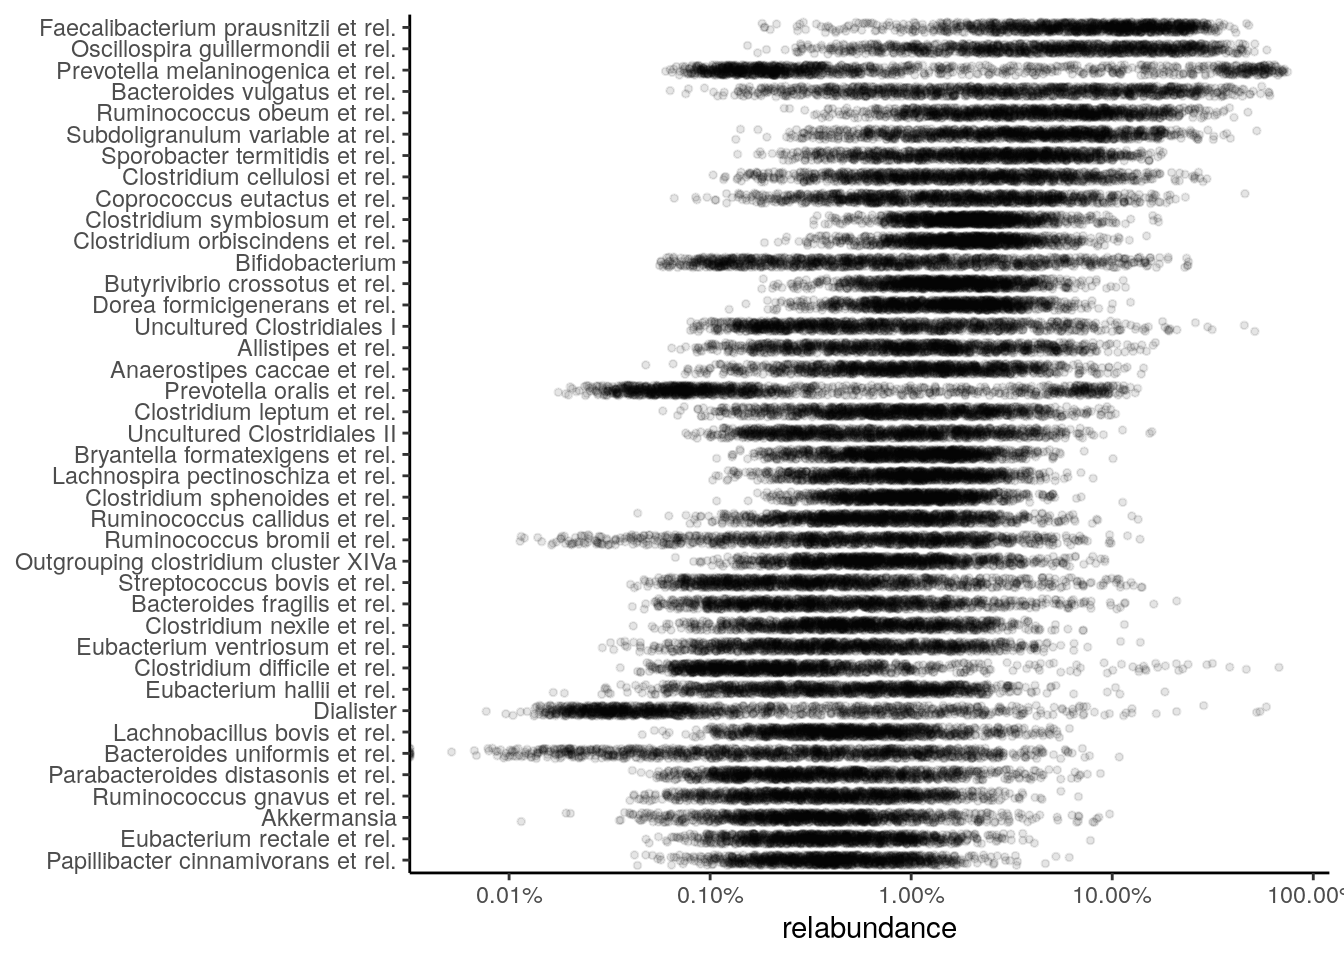
\includegraphics{12_quality_control_files/figure-latex/unnamed-chunk-2-1.pdf}

For instance, relative abundance values for the top 5 taxa can be
visualized as a density plot over a log scaled axis, using
``nationality'' as an overlaying information:

\begin{Shaded}
\begin{Highlighting}[]
\FunctionTok{plotAbundanceDensity}\NormalTok{(tse, }\AttributeTok{layout =} \StringTok{"density"}\NormalTok{, }\AttributeTok{abund\_values =} \StringTok{"relabundance"}\NormalTok{,}
                     \AttributeTok{n =} \DecValTok{5}\NormalTok{, }\AttributeTok{colour\_by=}\StringTok{"nationality"}\NormalTok{, }\AttributeTok{point\_alpha=}\DecValTok{1}\SpecialCharTok{/}\DecValTok{10}\NormalTok{ ) }\SpecialCharTok{+}
    \FunctionTok{scale\_x\_log10}\NormalTok{()}
\end{Highlighting}
\end{Shaded}

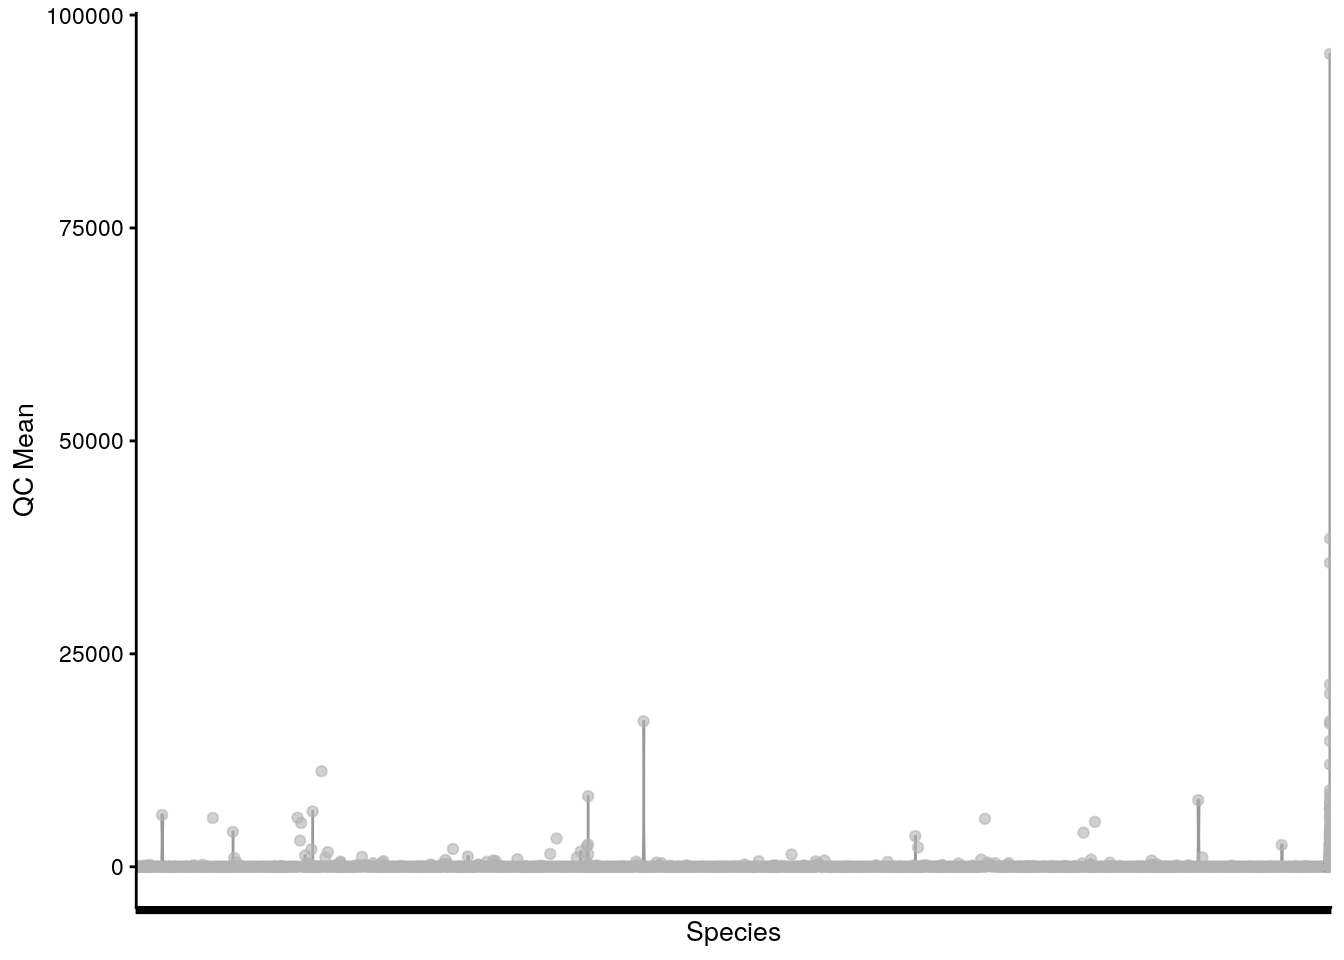
\includegraphics{12_quality_control_files/figure-latex/unnamed-chunk-3-1.pdf}

\hypertarget{prevalence}{%
\section{Prevalence}\label{prevalence}}

Prevalence is a measurement which describes in how many samples certain
microbes were detected.

Investigating the prevalence of microbes allows you either to focus on changes,
which pertain to most of the samples, or to focus on less often found microbes,
which are nonetheless abundantly found in a small number of samples.

On the raw data, the population prevalence (frequency) at a 1\% relative
abundance threshold (\texttt{detection\ =\ 1/100} and \texttt{as\_relative\ =\ TRUE}), can look
like this. The low prevalence in this example can be explained by rather
different sample types as well as the in-depth nature of the data.

\begin{Shaded}
\begin{Highlighting}[]
\FunctionTok{head}\NormalTok{(}\FunctionTok{getPrevalence}\NormalTok{(tse, }\AttributeTok{detection =} \DecValTok{1}\SpecialCharTok{/}\DecValTok{100}\NormalTok{, }\AttributeTok{sort =} \ConstantTok{TRUE}\NormalTok{, }\AttributeTok{as\_relative =} \ConstantTok{TRUE}\NormalTok{))}
\end{Highlighting}
\end{Shaded}

\begin{verbatim}
## Faecalibacterium prausnitzii et rel.           Ruminococcus obeum et rel. 
##                               0.9522                               0.9140 
##   Oscillospira guillermondii et rel.        Clostridium symbiosum et rel. 
##                               0.8801                               0.8714 
##     Subdoligranulum variable at rel.     Clostridium orbiscindens et rel. 
##                               0.8358                               0.8315
\end{verbatim}

The \texttt{detection} and \texttt{as\_relative} can also be used to access, how many samples
do pass a threshold for raw counts. Here the population prevalence (frequency)
at the absolute abundance threshold (\texttt{as\_relative\ =\ FALSE}) at read count 1
(\texttt{detection\ =\ 1}) is accessed.

\begin{Shaded}
\begin{Highlighting}[]
\FunctionTok{head}\NormalTok{(}\FunctionTok{getPrevalence}\NormalTok{(tse, }\AttributeTok{detection =} \DecValTok{1}\NormalTok{, }\AttributeTok{sort =} \ConstantTok{TRUE}\NormalTok{, }\AttributeTok{abund\_values =} \StringTok{"counts"}\NormalTok{,}
                   \AttributeTok{as\_relative =} \ConstantTok{FALSE}\NormalTok{))}
\end{Highlighting}
\end{Shaded}

\begin{verbatim}
##            Uncultured Mollicutes      Uncultured Clostridiales II 
##                                1                                1 
##       Uncultured Clostridiales I               Tannerella et rel. 
##                                1                                1 
##   Sutterella wadsworthia et rel. Subdoligranulum variable at rel. 
##                                1                                1
\end{verbatim}

Note that, if the output should be used for subsetting or storing the data in
the \texttt{rowData}, set \texttt{sort\ =\ FALSE}.

\hypertarget{prevalent-microbiota-analysis}{%
\subsection{Prevalent microbiota analysis}\label{prevalent-microbiota-analysis}}

To investigate the microbiome data at a selected taxonomic level, two
approaches are available.

First the data can be agglomerated to the taxonomic level and \texttt{getPrevalence}
be used on the result.

\begin{Shaded}
\begin{Highlighting}[]
\FunctionTok{altExp}\NormalTok{(tse,}\StringTok{"Phylum"}\NormalTok{) }\OtherTok{\textless{}{-}} \FunctionTok{agglomerateByRank}\NormalTok{(tse, }\StringTok{"Phylum"}\NormalTok{)}
\FunctionTok{head}\NormalTok{(}\FunctionTok{getPrevalence}\NormalTok{(}\FunctionTok{altExp}\NormalTok{(tse,}\StringTok{"Phylum"}\NormalTok{), }\AttributeTok{detection =} \DecValTok{1}\SpecialCharTok{/}\DecValTok{100}\NormalTok{, }\AttributeTok{sort =} \ConstantTok{TRUE}\NormalTok{,}
                   \AttributeTok{abund\_values =} \StringTok{"counts"}\NormalTok{, }\AttributeTok{as\_relative =} \ConstantTok{TRUE}\NormalTok{))}
\end{Highlighting}
\end{Shaded}

\begin{verbatim}
##      Firmicutes   Bacteroidetes  Actinobacteria  Proteobacteria Verrucomicrobia 
##       1.0000000       0.9852302       0.4821894       0.2988705       0.1277150 
##   Cyanobacteria 
##       0.0008688
\end{verbatim}

Alternatively, the \texttt{rank} argument can be set to perform the agglomeration on
the fly.

\begin{Shaded}
\begin{Highlighting}[]
\FunctionTok{altExp}\NormalTok{(tse,}\StringTok{"Phylum"}\NormalTok{) }\OtherTok{\textless{}{-}} \FunctionTok{agglomerateByRank}\NormalTok{(tse, }\StringTok{"Phylum"}\NormalTok{)}
\FunctionTok{head}\NormalTok{(}\FunctionTok{getPrevalence}\NormalTok{(tse, }\AttributeTok{rank =} \StringTok{"Phylum"}\NormalTok{, }\AttributeTok{detection =} \DecValTok{1}\SpecialCharTok{/}\DecValTok{100}\NormalTok{, }\AttributeTok{sort =} \ConstantTok{TRUE}\NormalTok{,}
                   \AttributeTok{abund\_values =} \StringTok{"counts"}\NormalTok{, }\AttributeTok{as\_relative =} \ConstantTok{TRUE}\NormalTok{))}
\end{Highlighting}
\end{Shaded}

\begin{verbatim}
##      Firmicutes   Bacteroidetes  Actinobacteria  Proteobacteria Verrucomicrobia 
##       1.0000000       0.9852302       0.4821894       0.2988705       0.1277150 
##   Cyanobacteria 
##       0.0008688
\end{verbatim}

The difference in the naming scheme is that, by default, \texttt{na.rm\ =\ TRUE} is used
for agglomeration in \texttt{getPrevalence}, whereas the default for
\texttt{agglomerateByRank} is \texttt{FALSE} to prevent accidental data loss.

If you only need the names of the prevalent taxa, \texttt{getPrevalentTaxa} is
available. This returns the taxa that exceed the given prevalence and detection
thresholds.

\begin{Shaded}
\begin{Highlighting}[]
\FunctionTok{getPrevalentTaxa}\NormalTok{(tse, }\AttributeTok{detection =} \DecValTok{0}\NormalTok{, }\AttributeTok{prevalence =} \DecValTok{50}\SpecialCharTok{/}\DecValTok{100}\NormalTok{)}
\NormalTok{prev }\OtherTok{\textless{}{-}} \FunctionTok{getPrevalentTaxa}\NormalTok{(tse, }\AttributeTok{detection =} \DecValTok{0}\NormalTok{, }\AttributeTok{prevalence =} \DecValTok{50}\SpecialCharTok{/}\DecValTok{100}\NormalTok{,}
                         \AttributeTok{rank =} \StringTok{"Phylum"}\NormalTok{, }\AttributeTok{sort =} \ConstantTok{TRUE}\NormalTok{)}
\NormalTok{prev}
\end{Highlighting}
\end{Shaded}

Note that the \texttt{detection} and \texttt{prevalence} thresholds are not the same, since
\texttt{detection} can be applied to relative counts or absolute counts depending on
whether \texttt{as\_relative} is set \texttt{TRUE} or \texttt{FALSE}

TODO
See also related functions for the analysis of rare and variable taxa (\texttt{rareMembers}; \texttt{rareAbundance}; \texttt{lowAbundance}).

Additional functions are available for abundance evaluation of prevalent taxa (\texttt{getPrevalentAbundance}) and analysis focused on rare taxa (\texttt{getRareTaxa}, \texttt{subsetByRareTaxa}).

\hypertarget{plotting-prevalence}{%
\subsection{Plotting prevalence}\label{plotting-prevalence}}

To plot the prevalence, the data is first added to the \texttt{rowData}.

\begin{Shaded}
\begin{Highlighting}[]
\FunctionTok{rowData}\NormalTok{(}\FunctionTok{altExp}\NormalTok{(tse,}\StringTok{"Phylum"}\NormalTok{))}\SpecialCharTok{$}\NormalTok{prevalence }\OtherTok{\textless{}{-}} 
    \FunctionTok{getPrevalence}\NormalTok{(}\FunctionTok{altExp}\NormalTok{(tse,}\StringTok{"Phylum"}\NormalTok{), }\AttributeTok{detection =} \DecValTok{1}\SpecialCharTok{/}\DecValTok{100}\NormalTok{, }\AttributeTok{sort =} \ConstantTok{FALSE}\NormalTok{,}
                  \AttributeTok{abund\_values =} \StringTok{"counts"}\NormalTok{, }\AttributeTok{as\_relative =} \ConstantTok{TRUE}\NormalTok{)}
\end{Highlighting}
\end{Shaded}

Then it can be plotted via the plotting functions from the \texttt{scater} package.

\begin{Shaded}
\begin{Highlighting}[]
\FunctionTok{library}\NormalTok{(scater)}
\FunctionTok{plotRowData}\NormalTok{(}\FunctionTok{altExp}\NormalTok{(tse,}\StringTok{"Phylum"}\NormalTok{), }\StringTok{"prevalence"}\NormalTok{, }\AttributeTok{colour\_by =} \StringTok{"Phylum"}\NormalTok{)}
\end{Highlighting}
\end{Shaded}

\includegraphics{12_quality_control_files/figure-latex/unnamed-chunk-7-1.pdf}

Additionally, the prevalence can be plotted on the taxonomic tree using the
\texttt{miaViz} package.

\begin{Shaded}
\begin{Highlighting}[]
\FunctionTok{altExps}\NormalTok{(tse) }\OtherTok{\textless{}{-}} \FunctionTok{splitByRanks}\NormalTok{(tse)}
\FunctionTok{altExps}\NormalTok{(tse) }\OtherTok{\textless{}{-}}
   \FunctionTok{lapply}\NormalTok{(}\FunctionTok{altExps}\NormalTok{(tse),}
          \ControlFlowTok{function}\NormalTok{(y)\{}
              \FunctionTok{rowData}\NormalTok{(y)}\SpecialCharTok{$}\NormalTok{prevalence }\OtherTok{\textless{}{-}} 
                  \FunctionTok{getPrevalence}\NormalTok{(y, }\AttributeTok{detection =} \DecValTok{1}\SpecialCharTok{/}\DecValTok{100}\NormalTok{, }\AttributeTok{sort =} \ConstantTok{FALSE}\NormalTok{,}
                                \AttributeTok{abund\_values =} \StringTok{"counts"}\NormalTok{, }\AttributeTok{as\_relative =} \ConstantTok{TRUE}\NormalTok{)}
\NormalTok{              y}
\NormalTok{          \})}
\NormalTok{top\_phyla }\OtherTok{\textless{}{-}} \FunctionTok{getTopTaxa}\NormalTok{(}\FunctionTok{altExp}\NormalTok{(tse,}\StringTok{"Phylum"}\NormalTok{),}
                        \AttributeTok{method=}\StringTok{"prevalence"}\NormalTok{,}
                        \AttributeTok{top=}\NormalTok{5L,}
                        \AttributeTok{abund\_values=}\StringTok{"counts"}\NormalTok{)}
\NormalTok{top\_phyla\_mean }\OtherTok{\textless{}{-}} \FunctionTok{getTopTaxa}\NormalTok{(}\FunctionTok{altExp}\NormalTok{(tse,}\StringTok{"Phylum"}\NormalTok{),}
                             \AttributeTok{method=}\StringTok{"mean"}\NormalTok{,}
                             \AttributeTok{top=}\NormalTok{5L,}
                             \AttributeTok{abund\_values=}\StringTok{"counts"}\NormalTok{)}
\NormalTok{x }\OtherTok{\textless{}{-}} \FunctionTok{unsplitByRanks}\NormalTok{(tse, }\AttributeTok{ranks =} \FunctionTok{taxonomyRanks}\NormalTok{(tse)[}\DecValTok{1}\SpecialCharTok{:}\DecValTok{6}\NormalTok{])}
\NormalTok{x }\OtherTok{\textless{}{-}} \FunctionTok{addTaxonomyTree}\NormalTok{(x)}
\end{Highlighting}
\end{Shaded}

After some preparation the data is assembled and can be plotted via
\texttt{plotRowTree}.

\begin{Shaded}
\begin{Highlighting}[]
\FunctionTok{library}\NormalTok{(miaViz)}
\FunctionTok{plotRowTree}\NormalTok{(x[}\FunctionTok{rowData}\NormalTok{(x)}\SpecialCharTok{$}\NormalTok{Phylum }\SpecialCharTok{\%in\%}\NormalTok{ top\_phyla,],}
            \AttributeTok{edge\_colour\_by =} \StringTok{"Phylum"}\NormalTok{,}
            \AttributeTok{tip\_colour\_by =} \StringTok{"prevalence"}\NormalTok{,}
            \AttributeTok{node\_colour\_by =} \StringTok{"prevalence"}\NormalTok{)}
\end{Highlighting}
\end{Shaded}

\begin{figure}
\centering
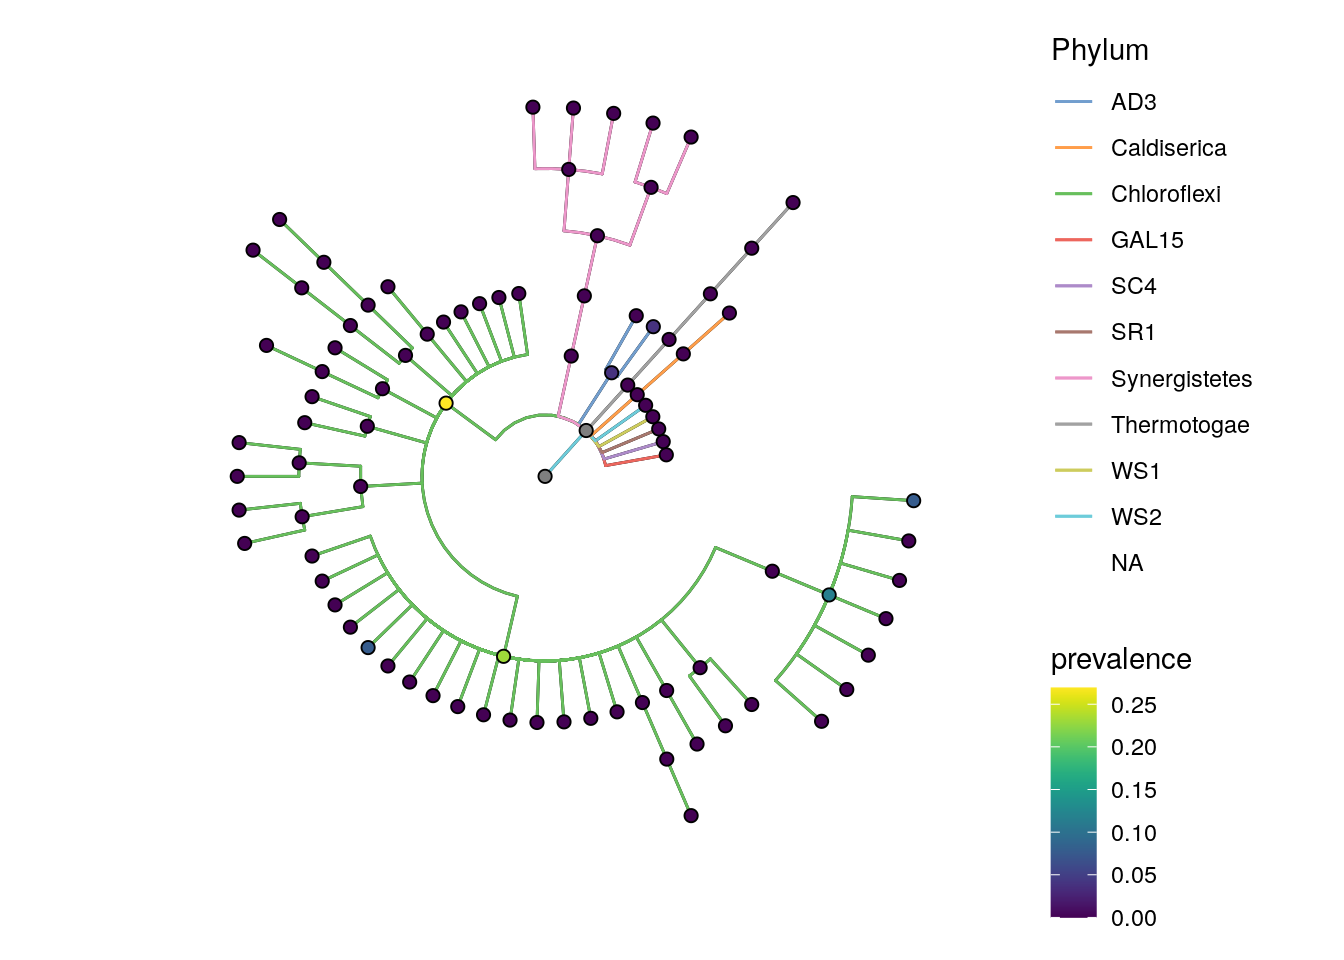
\includegraphics{12_quality_control_files/figure-latex/plot-prev-prev-1.pdf}
\caption{\label{fig:plot-prev-prev}Prevalence of top phyla as judged by prevalence}
\end{figure}

\begin{Shaded}
\begin{Highlighting}[]
\FunctionTok{plotRowTree}\NormalTok{(x[}\FunctionTok{rowData}\NormalTok{(x)}\SpecialCharTok{$}\NormalTok{Phylum }\SpecialCharTok{\%in\%}\NormalTok{ top\_phyla\_mean,],}
            \AttributeTok{edge\_colour\_by =} \StringTok{"Phylum"}\NormalTok{,}
            \AttributeTok{tip\_colour\_by =} \StringTok{"prevalence"}\NormalTok{,}
            \AttributeTok{node\_colour\_by =} \StringTok{"prevalence"}\NormalTok{)}
\end{Highlighting}
\end{Shaded}

\begin{figure}
\centering
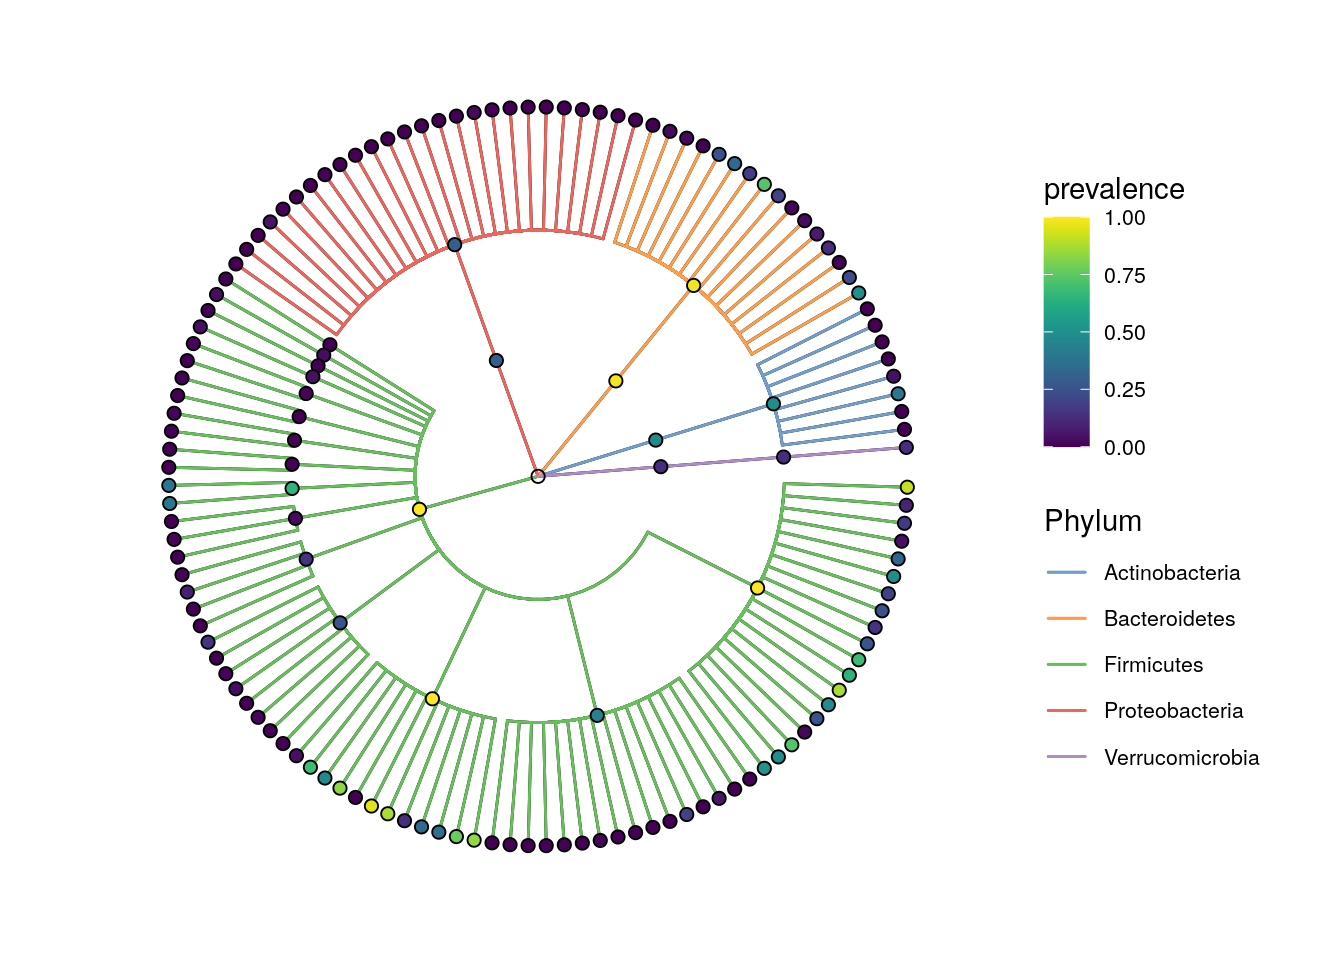
\includegraphics{12_quality_control_files/figure-latex/plot-prev-mean-1.pdf}
\caption{\label{fig:plot-prev-mean}Prevalence of top phyla as judged by mean abundance}
\end{figure}

\hypertarget{quality-control-1}{%
\section{Quality control}\label{quality-control-1}}

\begin{Shaded}
\begin{Highlighting}[]
\FunctionTok{library}\NormalTok{(mia)}
\FunctionTok{data}\NormalTok{(}\StringTok{"GlobalPatterns"}\NormalTok{, }\AttributeTok{package=}\StringTok{"mia"}\NormalTok{)}
\NormalTok{tse }\OtherTok{\textless{}{-}}\NormalTok{ GlobalPatterns }
\end{Highlighting}
\end{Shaded}

\hypertarget{top-taxa}{%
\subsection{Top taxa}\label{top-taxa}}

The \texttt{getTopTaxa} can be used for identifying top taxa in the data.

\begin{Shaded}
\begin{Highlighting}[]
\NormalTok{top\_features }\OtherTok{\textless{}{-}} \FunctionTok{getTopTaxa}\NormalTok{(tse, }\AttributeTok{method=}\StringTok{"median"}\NormalTok{, }\AttributeTok{top=}\DecValTok{10}\NormalTok{)}
\NormalTok{tax\_data }\OtherTok{\textless{}{-}} \FunctionTok{rowData}\NormalTok{(tse)[top\_features,}\FunctionTok{taxonomyRanks}\NormalTok{(tse)]}
\NormalTok{tax\_data}
\end{Highlighting}
\end{Shaded}

\begin{verbatim}
## DataFrame with 10 rows and 7 columns
##            Kingdom         Phylum               Class             Order
##        <character>    <character>         <character>       <character>
## 549656    Bacteria  Cyanobacteria         Chloroplast     Stramenopiles
## 331820    Bacteria  Bacteroidetes         Bacteroidia     Bacteroidales
## 317182    Bacteria  Cyanobacteria         Chloroplast     Stramenopiles
## 94166     Bacteria Proteobacteria Gammaproteobacteria    Pasteurellales
## 279599    Bacteria  Cyanobacteria    Nostocophycideae        Nostocales
## 158660    Bacteria  Bacteroidetes         Bacteroidia     Bacteroidales
## 329744    Bacteria Actinobacteria      Actinobacteria   Actinomycetales
## 326977    Bacteria Actinobacteria      Actinobacteria Bifidobacteriales
## 248140    Bacteria  Bacteroidetes         Bacteroidia     Bacteroidales
## 550960    Bacteria Proteobacteria Gammaproteobacteria Enterobacteriales
##                    Family           Genus                Species
##               <character>     <character>            <character>
## 549656                 NA              NA                     NA
## 331820     Bacteroidaceae     Bacteroides                     NA
## 317182                 NA              NA                     NA
## 94166     Pasteurellaceae     Haemophilus Haemophilusparainflu..
## 279599        Nostocaceae  Dolichospermum                     NA
## 158660     Bacteroidaceae     Bacteroides                     NA
## 329744             ACK-M1              NA                     NA
## 326977 Bifidobacteriaceae Bifidobacterium Bifidobacteriumadole..
## 248140     Bacteroidaceae     Bacteroides      Bacteroidescaccae
## 550960 Enterobacteriaceae     Providencia                     NA
\end{verbatim}

\hypertarget{library-size}{%
\subsection{Library size}\label{library-size}}

The total counts/sample can be calculated using the
\texttt{perCellQCMetrics}/\texttt{addPerCellQC} from the \texttt{scater} package. The former one
just calculates the values, whereas the latter one directly adds them to the
\texttt{colData}.

\begin{Shaded}
\begin{Highlighting}[]
\FunctionTok{library}\NormalTok{(scater)}
\FunctionTok{perCellQCMetrics}\NormalTok{(tse)}
\end{Highlighting}
\end{Shaded}

\begin{verbatim}
## DataFrame with 26 rows and 3 columns
##               sum  detected     total
##         <numeric> <numeric> <numeric>
## CL3        864077      6964    864077
## CC1       1135457      7679   1135457
## SV1        697509      5729    697509
## M31Fcsw   1543451      2667   1543451
## M11Fcsw   2076476      2574   2076476
## ...           ...       ...       ...
## TS28       937466      2679    937466
## TS29      1211071      2629   1211071
## Even1     1216137      4213   1216137
## Even2      971073      3130    971073
## Even3     1078241      2776   1078241
\end{verbatim}

\begin{Shaded}
\begin{Highlighting}[]
\NormalTok{tse }\OtherTok{\textless{}{-}} \FunctionTok{addPerCellQC}\NormalTok{(tse)}
\FunctionTok{colData}\NormalTok{(tse)}
\end{Highlighting}
\end{Shaded}

\begin{verbatim}
## DataFrame with 26 rows and 10 columns
##         X.SampleID   Primer Final_Barcode Barcode_truncated_plus_T
##           <factor> <factor>      <factor>                 <factor>
## CL3        CL3      ILBC_01        AACGCA                   TGCGTT
## CC1        CC1      ILBC_02        AACTCG                   CGAGTT
## SV1        SV1      ILBC_03        AACTGT                   ACAGTT
## M31Fcsw    M31Fcsw  ILBC_04        AAGAGA                   TCTCTT
## M11Fcsw    M11Fcsw  ILBC_05        AAGCTG                   CAGCTT
## ...            ...      ...           ...                      ...
## TS28         TS28   ILBC_25        ACCAGA                   TCTGGT
## TS29         TS29   ILBC_26        ACCAGC                   GCTGGT
## Even1        Even1  ILBC_27        ACCGCA                   TGCGGT
## Even2        Even2  ILBC_28        ACCTCG                   CGAGGT
## Even3        Even3  ILBC_29        ACCTGT                   ACAGGT
##         Barcode_full_length SampleType
##                    <factor>   <factor>
## CL3             CTAGCGTGCGT      Soil 
## CC1             CATCGACGAGT      Soil 
## SV1             GTACGCACAGT      Soil 
## M31Fcsw         TCGACATCTCT      Feces
## M11Fcsw         CGACTGCAGCT      Feces
## ...                     ...        ...
## TS28            GCATCGTCTGG      Feces
## TS29            CTAGTCGCTGG      Feces
## Even1           TGACTCTGCGG      Mock 
## Even2           TCTGATCGAGG      Mock 
## Even3           AGAGAGACAGG      Mock 
##                                        Description       sum  detected
##                                           <factor> <numeric> <numeric>
## CL3     Calhoun South Carolina Pine soil, pH 4.9      864077      6964
## CC1     Cedar Creek Minnesota, grassland, pH 6.1     1135457      7679
## SV1     Sevilleta new Mexico, desert scrub, pH 8.3    697509      5729
## M31Fcsw M3, Day 1, fecal swab, whole body study      1543451      2667
## M11Fcsw M1, Day 1, fecal swab, whole body study      2076476      2574
## ...                                            ...       ...       ...
## TS28                                       Twin #1    937466      2679
## TS29                                       Twin #2   1211071      2629
## Even1                                      Even1     1216137      4213
## Even2                                      Even2      971073      3130
## Even3                                      Even3     1078241      2776
##             total
##         <numeric>
## CL3        864077
## CC1       1135457
## SV1        697509
## M31Fcsw   1543451
## M11Fcsw   2076476
## ...           ...
## TS28       937466
## TS29      1211071
## Even1     1216137
## Even2      971073
## Even3     1078241
\end{verbatim}

The distribution of calculated library sizes can be visualized as a
histogram (left), or by sorting the samples by library size (right).

\begin{Shaded}
\begin{Highlighting}[]
\FunctionTok{library}\NormalTok{(ggplot2)}

\NormalTok{p1 }\OtherTok{\textless{}{-}} \FunctionTok{ggplot}\NormalTok{(}\FunctionTok{as.data.frame}\NormalTok{(}\FunctionTok{colData}\NormalTok{(tse))) }\SpecialCharTok{+}
        \FunctionTok{geom\_histogram}\NormalTok{(}\FunctionTok{aes}\NormalTok{(}\AttributeTok{x =}\NormalTok{ sum), }\AttributeTok{color =} \StringTok{"black"}\NormalTok{, }\AttributeTok{fill =} \StringTok{"gray"}\NormalTok{, }\AttributeTok{bins =} \DecValTok{30}\NormalTok{) }\SpecialCharTok{+}
        \FunctionTok{labs}\NormalTok{(}\AttributeTok{x =} \StringTok{"Library size"}\NormalTok{, }\AttributeTok{y =} \StringTok{"Frequency (n)"}\NormalTok{) }\SpecialCharTok{+} 
        \CommentTok{\# scale\_x\_log10(breaks = scales::trans\_breaks("log10", function(x) 10\^{}x), }
        \CommentTok{\# labels = scales::trans\_format("log10", scales::math\_format(10\^{}.x))) +}
        \FunctionTok{theme\_bw}\NormalTok{() }\SpecialCharTok{+}
        \FunctionTok{theme}\NormalTok{(}\AttributeTok{panel.grid.major =} \FunctionTok{element\_blank}\NormalTok{(), }\CommentTok{\# Removes the grid}
          \AttributeTok{panel.grid.minor =} \FunctionTok{element\_blank}\NormalTok{(),}
          \AttributeTok{panel.border =} \FunctionTok{element\_blank}\NormalTok{(),}
          \AttributeTok{panel.background =} \FunctionTok{element\_blank}\NormalTok{(),}
          \AttributeTok{axis.line =} \FunctionTok{element\_line}\NormalTok{(}\AttributeTok{colour =} \StringTok{"black"}\NormalTok{)) }\CommentTok{\# Adds y{-}axis}

\FunctionTok{library}\NormalTok{(dplyr)}
\NormalTok{df }\OtherTok{\textless{}{-}} \FunctionTok{as.data.frame}\NormalTok{(}\FunctionTok{colData}\NormalTok{(tse)) }\SpecialCharTok{\%\textgreater{}\%}
        \FunctionTok{arrange}\NormalTok{(sum) }\SpecialCharTok{\%\textgreater{}\%}
        \FunctionTok{mutate}\NormalTok{(}\AttributeTok{index =} \DecValTok{1}\SpecialCharTok{:}\FunctionTok{n}\NormalTok{())}
\NormalTok{p2 }\OtherTok{\textless{}{-}} \FunctionTok{ggplot}\NormalTok{(df, }\FunctionTok{aes}\NormalTok{(}\AttributeTok{y =}\NormalTok{ index, }\AttributeTok{x =}\NormalTok{ sum}\SpecialCharTok{/}\FloatTok{1e6}\NormalTok{)) }\SpecialCharTok{+}
        \FunctionTok{geom\_point}\NormalTok{() }\SpecialCharTok{+}  
        \FunctionTok{labs}\NormalTok{(}\AttributeTok{x =} \StringTok{"Library size (million reads)"}\NormalTok{, }\AttributeTok{y =} \StringTok{"Sample index"}\NormalTok{) }\SpecialCharTok{+}  
        \FunctionTok{theme\_bw}\NormalTok{() }\SpecialCharTok{+}
        \FunctionTok{theme}\NormalTok{(}\AttributeTok{panel.grid.major =} \FunctionTok{element\_blank}\NormalTok{(), }\CommentTok{\# Removes the grid}
          \AttributeTok{panel.grid.minor =} \FunctionTok{element\_blank}\NormalTok{(),}
          \AttributeTok{panel.border =} \FunctionTok{element\_blank}\NormalTok{(),}
          \AttributeTok{panel.background =} \FunctionTok{element\_blank}\NormalTok{(),}
          \AttributeTok{axis.line =} \FunctionTok{element\_line}\NormalTok{(}\AttributeTok{colour =} \StringTok{"black"}\NormalTok{)) }\CommentTok{\# Adds y{-}axis}

\FunctionTok{library}\NormalTok{(patchwork)}
\NormalTok{p1 }\SpecialCharTok{+}\NormalTok{ p2}
\end{Highlighting}
\end{Shaded}

\begin{figure}
\centering
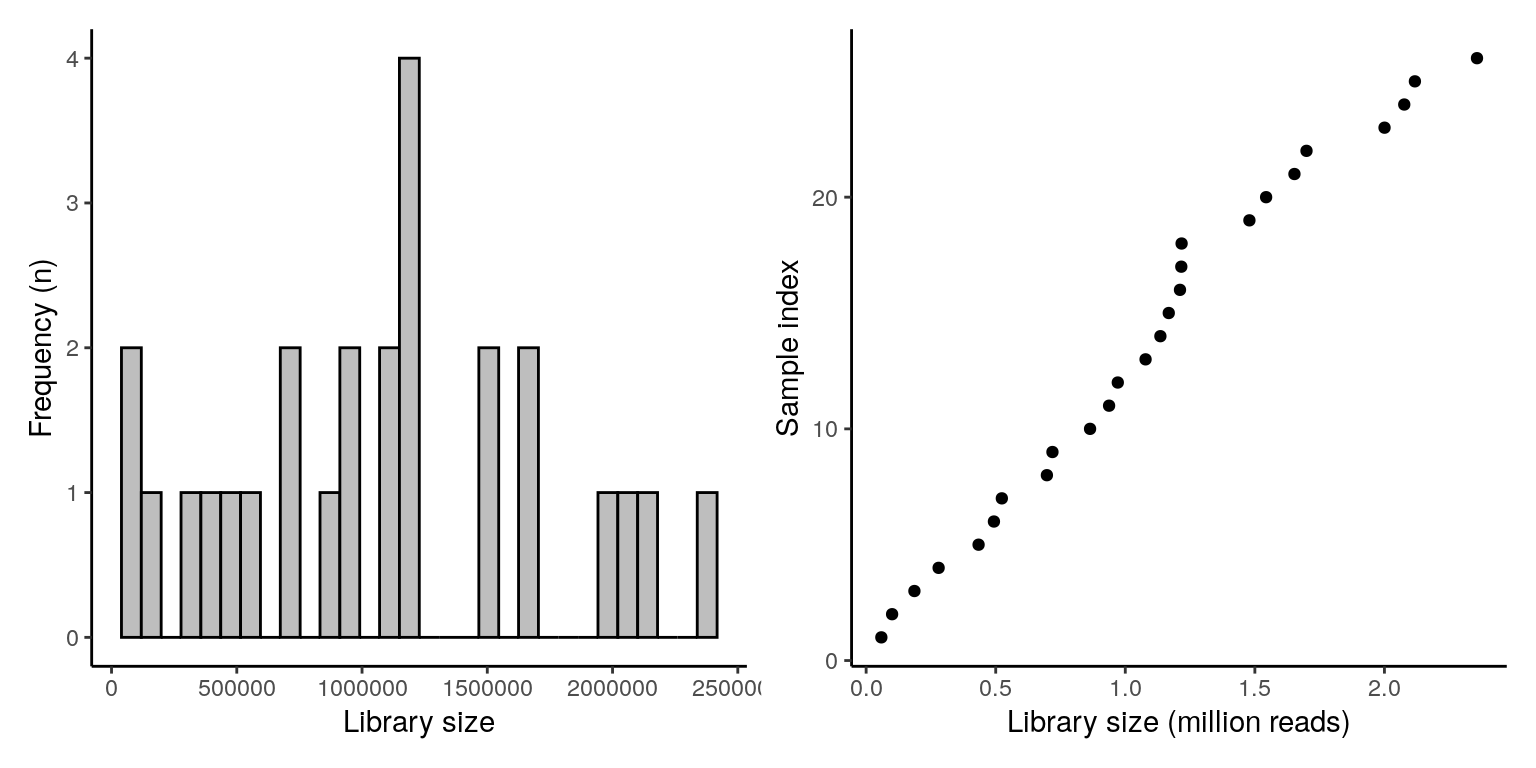
\includegraphics{12_quality_control_files/figure-latex/plot-viz-lib-size-1-1.pdf}
\caption{\label{fig:plot-viz-lib-size-1}Library size distribution.}
\end{figure}

Library sizes - and other variables from \texttt{colData} - can be also visualized by using
specified function called \texttt{plotColData}.

\begin{Shaded}
\begin{Highlighting}[]
\FunctionTok{library}\NormalTok{(ggplot2)}
\CommentTok{\# Sort samples by read count, order the factor levels, and store back to tse as DataFrame}
\CommentTok{\# }\AlertTok{TODO}\CommentTok{: plotColData could include an option for sorting samples based on colData variables}
\FunctionTok{colData}\NormalTok{(tse) }\OtherTok{\textless{}{-}} \FunctionTok{as.data.frame}\NormalTok{(}\FunctionTok{colData}\NormalTok{(tse)) }\SpecialCharTok{\%\textgreater{}\%}
                 \FunctionTok{arrange}\NormalTok{(X.SampleID) }\SpecialCharTok{\%\textgreater{}\%}
             \FunctionTok{mutate}\NormalTok{(}\AttributeTok{X.SampleID =} \FunctionTok{factor}\NormalTok{(X.SampleID, }\AttributeTok{levels=}\NormalTok{X.SampleID)) }\SpecialCharTok{\%\textgreater{}\%}
\NormalTok{         DataFrame}
\FunctionTok{plotColData}\NormalTok{(tse,}\StringTok{"sum"}\NormalTok{,}\StringTok{"X.SampleID"}\NormalTok{, }\AttributeTok{colour\_by =} \StringTok{"SampleType"}\NormalTok{) }\SpecialCharTok{+} 
    \FunctionTok{theme}\NormalTok{(}\AttributeTok{axis.text.x =} \FunctionTok{element\_text}\NormalTok{(}\AttributeTok{angle =} \DecValTok{45}\NormalTok{, }\AttributeTok{hjust=}\DecValTok{1}\NormalTok{)) }\SpecialCharTok{+}
    \FunctionTok{labs}\NormalTok{(}\AttributeTok{y =} \StringTok{"Library size (N)"}\NormalTok{, }\AttributeTok{x =} \StringTok{"Sample ID"}\NormalTok{)       }
\end{Highlighting}
\end{Shaded}

\begin{figure}
\centering
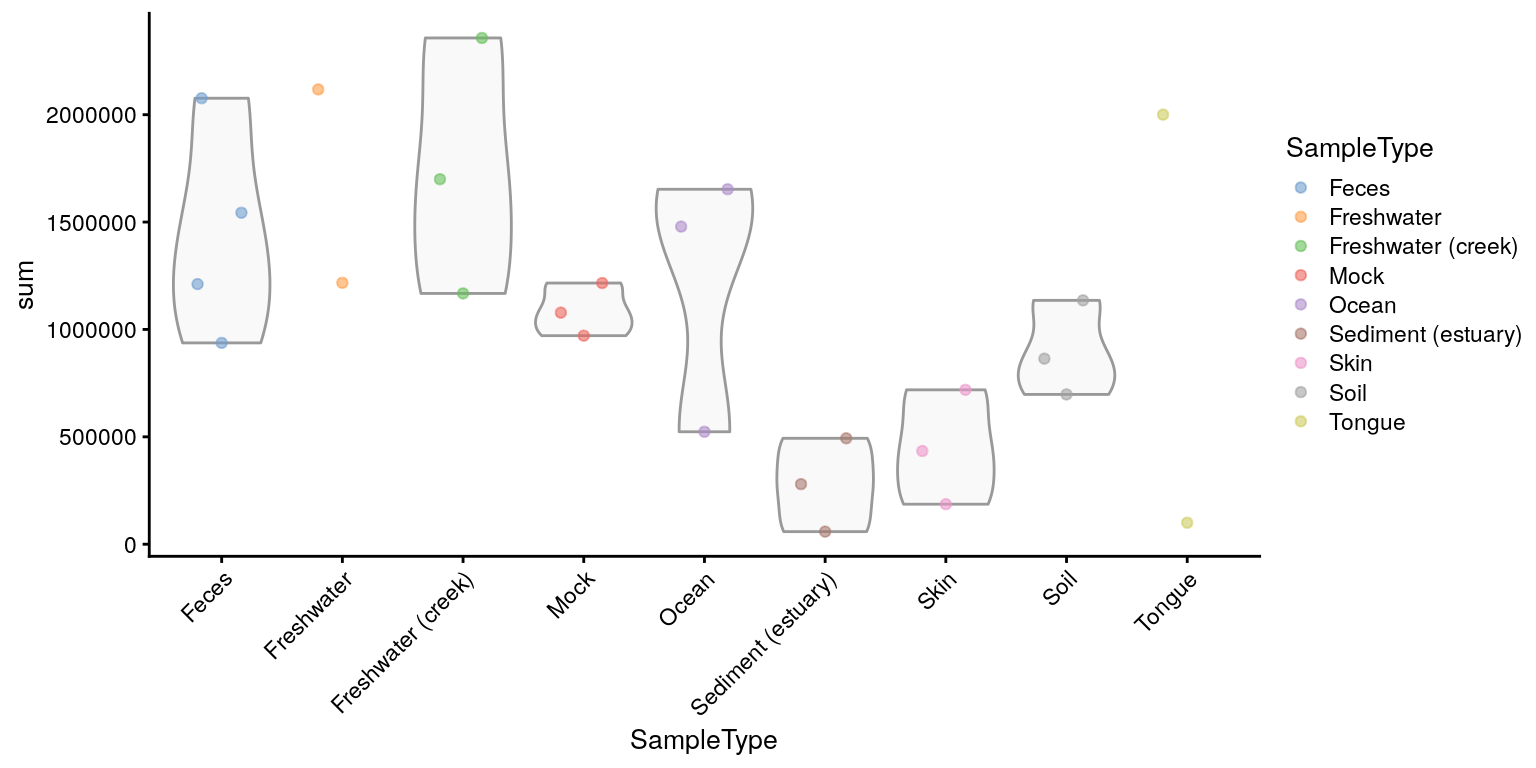
\includegraphics{12_quality_control_files/figure-latex/plot-viz-lib-size-2-1.pdf}
\caption{\label{fig:plot-viz-lib-size-2}Library sizes per sample.}
\end{figure}

\begin{Shaded}
\begin{Highlighting}[]
\FunctionTok{plotColData}\NormalTok{(tse,}\StringTok{"sum"}\NormalTok{,}\StringTok{"SampleType"}\NormalTok{, }\AttributeTok{colour\_by =} \StringTok{"SampleType"}\NormalTok{) }\SpecialCharTok{+} 
    \FunctionTok{theme}\NormalTok{(}\AttributeTok{axis.text.x =} \FunctionTok{element\_text}\NormalTok{(}\AttributeTok{angle =} \DecValTok{45}\NormalTok{, }\AttributeTok{hjust=}\DecValTok{1}\NormalTok{))}
\end{Highlighting}
\end{Shaded}

\begin{figure}
\centering
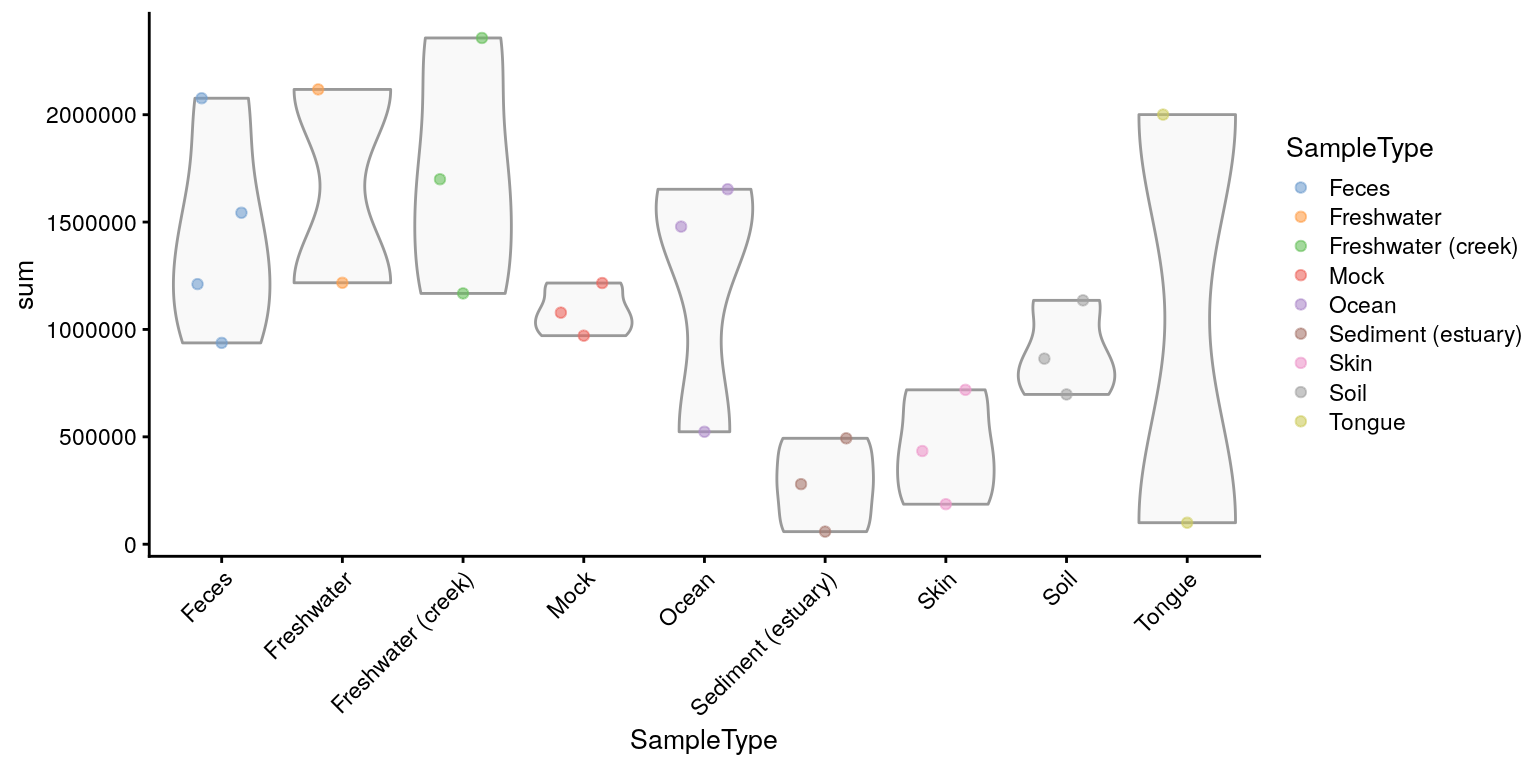
\includegraphics{12_quality_control_files/figure-latex/plot-viz-lib-size-3-1.pdf}
\caption{\label{fig:plot-viz-lib-size-3}Library sizes per sample type.}
\end{figure}

In addition, data can be rarefied with \href{https://microbiome.github.io/mia/reference/subsampleCounts.html}{subsampleCounts}, which normalises the samples to an equal number of reads. However, this practice is discouraged for the analysis of differentially abundant microorganisms (see \citep{mcmurdie2014waste}).

\hypertarget{contaminant-sequences}{%
\subsection{Contaminant sequences}\label{contaminant-sequences}}

Samples might be contaminated with exogenous sequences. The impact of each contaminant can be estimated based on their frequencies and concentrations across the samples.

The following \href{https://microbiome.github.io/mia/reference/isContaminant.html}{decontam functions} are based on the \citep{davis2018simple} and support such functionality:
* \texttt{isContaminant}, \texttt{isNotContaminant}
* \texttt{addContaminantQC}, \texttt{addNotContaminantQC}

\hypertarget{session-info-2}{%
\section*{Session Info}\label{session-info-2}}
\addcontentsline{toc}{section}{Session Info}

View session info

\begin{verbatim}
R version 4.1.2 (2021-11-01)
Platform: x86_64-pc-linux-gnu (64-bit)
Running under: Ubuntu 20.04.3 LTS

Matrix products: default
BLAS/LAPACK: /usr/lib/x86_64-linux-gnu/openblas-pthread/libopenblasp-r0.3.8.so

locale:
 [1] LC_CTYPE=en_US.UTF-8       LC_NUMERIC=C              
 [3] LC_TIME=en_US.UTF-8        LC_COLLATE=en_US.UTF-8    
 [5] LC_MONETARY=en_US.UTF-8    LC_MESSAGES=en_US.UTF-8   
 [7] LC_PAPER=en_US.UTF-8       LC_NAME=C                 
 [9] LC_ADDRESS=C               LC_TELEPHONE=C            
[11] LC_MEASUREMENT=en_US.UTF-8 LC_IDENTIFICATION=C       

attached base packages:
[1] stats4    stats     graphics  grDevices utils     datasets  methods  
[8] base     

other attached packages:
 [1] patchwork_1.1.1                dplyr_1.0.8                   
 [3] scater_1.22.0                  scuttle_1.4.0                 
 [5] miaViz_1.3.3                   ggraph_2.0.5                  
 [7] ggplot2_3.3.5                  microbiomeDataSets_1.1.5      
 [9] mia_1.3.19                     MultiAssayExperiment_1.20.0   
[11] TreeSummarizedExperiment_2.1.4 Biostrings_2.62.0             
[13] XVector_0.34.0                 SingleCellExperiment_1.16.0   
[15] SummarizedExperiment_1.24.0    Biobase_2.54.0                
[17] GenomicRanges_1.46.1           GenomeInfoDb_1.30.1           
[19] IRanges_2.28.0                 S4Vectors_0.32.3              
[21] BiocGenerics_0.40.0            MatrixGenerics_1.6.0          
[23] matrixStats_0.61.0-9001        BiocStyle_2.22.0              
[25] rebook_1.4.0                  

loaded via a namespace (and not attached):
  [1] AnnotationHub_3.2.2           BiocFileCache_2.2.1          
  [3] igraph_1.2.11                 plyr_1.8.6                   
  [5] lazyeval_0.2.2                splines_4.1.2                
  [7] BiocParallel_1.28.3           digest_0.6.29                
  [9] yulab.utils_0.0.4             htmltools_0.5.2              
 [11] viridis_0.6.2                 fansi_1.0.2                  
 [13] magrittr_2.0.2                memoise_2.0.1                
 [15] ScaledMatrix_1.2.0            cluster_2.1.2                
 [17] DECIPHER_2.22.0               graphlayouts_0.8.0           
 [19] colorspace_2.0-3              blob_1.2.2                   
 [21] rappdirs_0.3.3                ggrepel_0.9.1                
 [23] xfun_0.30                     crayon_1.5.0                 
 [25] RCurl_1.98-1.6                jsonlite_1.8.0               
 [27] graph_1.72.0                  ape_5.6-2                    
 [29] glue_1.6.2                    polyclip_1.10-0              
 [31] gtable_0.3.0                  zlibbioc_1.40.0              
 [33] DelayedArray_0.20.0           BiocSingular_1.10.0          
 [35] scales_1.1.1                  DBI_1.1.2                    
 [37] Rcpp_1.0.8.3                  viridisLite_0.4.0            
 [39] xtable_1.8-4                  decontam_1.14.0              
 [41] gridGraphics_0.5-1            tidytree_0.3.9               
 [43] bit_4.0.4                     rsvd_1.0.5                   
 [45] httr_1.4.2                    dir.expiry_1.2.0             
 [47] ellipsis_0.3.2                farver_2.1.0                 
 [49] pkgconfig_2.0.3               XML_3.99-0.9                 
 [51] CodeDepends_0.6.5             dbplyr_2.1.1                 
 [53] utf8_1.2.2                    labeling_0.4.2               
 [55] ggplotify_0.1.0               tidyselect_1.1.2             
 [57] rlang_1.0.2                   reshape2_1.4.4               
 [59] later_1.3.0                   AnnotationDbi_1.56.2         
 [61] munsell_0.5.0                 BiocVersion_3.14.0           
 [63] tools_4.1.2                   cachem_1.0.6                 
 [65] cli_3.2.0                     DirichletMultinomial_1.36.0  
 [67] generics_0.1.2                RSQLite_2.2.10               
 [69] ExperimentHub_2.2.1           evaluate_0.15                
 [71] stringr_1.4.0                 fastmap_1.1.0                
 [73] yaml_2.3.5                    ggtree_3.2.1                 
 [75] knitr_1.37                    bit64_4.0.5                  
 [77] tidygraph_1.2.0               purrr_0.3.4                  
 [79] KEGGREST_1.34.0               nlme_3.1-155                 
 [81] sparseMatrixStats_1.6.0       mime_0.12                    
 [83] aplot_0.1.2                   compiler_4.1.2               
 [85] beeswarm_0.4.0                filelock_1.0.2               
 [87] curl_4.3.2                    png_0.1-7                    
 [89] interactiveDisplayBase_1.32.0 treeio_1.18.1                
 [91] tweenr_1.0.2                  tibble_3.1.6                 
 [93] stringi_1.7.6                 highr_0.9                    
 [95] lattice_0.20-45               Matrix_1.4-0                 
 [97] vegan_2.5-7                   permute_0.9-7                
 [99] vctrs_0.3.8                   pillar_1.7.0                 
[101] lifecycle_1.0.1               BiocManager_1.30.16          
[103] BiocNeighbors_1.12.0          cowplot_1.1.1                
[105] bitops_1.0-7                  irlba_2.3.5                  
[107] httpuv_1.6.5                  R6_2.5.1                     
[109] bookdown_0.25                 promises_1.2.0.1             
[111] gridExtra_2.3                 vipor_0.4.5                  
[113] codetools_0.2-18              MASS_7.3-55                  
[115] assertthat_0.2.1              withr_2.5.0                  
[117] GenomeInfoDbData_1.2.7        mgcv_1.8-39                  
[119] parallel_4.1.2                ggfun_0.0.5                  
[121] grid_4.1.2                    beachmat_2.10.0              
[123] tidyr_1.2.0                   rmarkdown_2.13               
[125] DelayedMatrixStats_1.16.0     ggnewscale_0.4.6             
[127] ggforce_0.3.3                 shiny_1.7.1                  
[129] ggbeeswarm_0.6.0             
\end{verbatim}

\hypertarget{taxonomic-information}{%
\chapter{Taxonomic Information}\label{taxonomic-information}}

\begin{Shaded}
\begin{Highlighting}[]
\FunctionTok{library}\NormalTok{(mia)}
\FunctionTok{data}\NormalTok{(}\StringTok{"GlobalPatterns"}\NormalTok{, }\AttributeTok{package=}\StringTok{"mia"}\NormalTok{)}
\NormalTok{tse }\OtherTok{\textless{}{-}}\NormalTok{ GlobalPatterns }
\end{Highlighting}
\end{Shaded}

Taxonomic information is a key part of analyzing microbiome data and without
it, any type of data analysis probably will not make much sense. However,
the degree of detail of taxonomic information differs depending on the dataset
and annotation data used.

Therefore, the mia package expects a loose assembly of taxonomic information
and assumes certain key aspects:

\begin{itemize}
\tightlist
\item
  Taxonomic information is given as character vectors or factors in the
  \texttt{rowData} of a \texttt{SummarizedExperiment} object.
\item
  The columns containing the taxonomic information must be named \texttt{domain},
  \texttt{kingdom}, \texttt{phylum}, \texttt{class}, \texttt{order}, \texttt{family}, \texttt{genus}, \texttt{species} or with
  a capital first letter.
\item
  the columns must be given in the order shown above
\item
  column can be omited, but the order must remain
\end{itemize}

\hypertarget{assigning-taxonomic-information.}{%
\section{Assigning taxonomic information.}\label{assigning-taxonomic-information.}}

There are a number of methods to assign taxonomic information. We like to give
a short introduction about the methods available without ranking one over the
other. This has to be your choice based on the result for the individual
dataset.

\hypertarget{dada2}{%
\subsection{dada2}\label{dada2}}

The dada2 package \citep{R-dada2} implements the \texttt{assignTaxonomy} function, which
takes as input the ASV sequences associated with each row of data and a training
dataset. For more information visit the
\href{https://benjjneb.github.io/dada2/assign.html}{dada2 homepage}.

\hypertarget{decipher}{%
\subsection{DECIPHER}\label{decipher}}

The DECIPHER package \citep{R-DECIPHER} implements the \texttt{IDTAXA} algorithm to assign
either taxonomic information or function information. For \texttt{mia}
only the first option is of interest for now and more information can be
found on the \href{http://www2.decipher.codes/Classification.html}{DECIPHER website}.

\hypertarget{functions-to-access-taxonomic-information}{%
\section{Functions to access taxonomic information}\label{functions-to-access-taxonomic-information}}

\texttt{checkTaxonomy} checks whether the taxonomic information is usable for \texttt{mia}

\begin{Shaded}
\begin{Highlighting}[]
\FunctionTok{checkTaxonomy}\NormalTok{(tse)}
\end{Highlighting}
\end{Shaded}

\begin{verbatim}
## [1] TRUE
\end{verbatim}

Since the \texttt{rowData} can contain other data, \texttt{taxonomyRanks} will return the
columns \texttt{mia} assumes to contain the taxonomic information.

\begin{Shaded}
\begin{Highlighting}[]
\FunctionTok{taxonomyRanks}\NormalTok{(tse)}
\end{Highlighting}
\end{Shaded}

\begin{verbatim}
## [1] "Kingdom" "Phylum"  "Class"   "Order"   "Family"  "Genus"   "Species"
\end{verbatim}

This can then be used to subset the \texttt{rowData} to columns needed.

\begin{Shaded}
\begin{Highlighting}[]
\FunctionTok{rowData}\NormalTok{(tse)[,}\FunctionTok{taxonomyRanks}\NormalTok{(tse)]}
\end{Highlighting}
\end{Shaded}

\begin{verbatim}
## DataFrame with 19216 rows and 7 columns
##            Kingdom        Phylum        Class        Order        Family
##        <character>   <character>  <character>  <character>   <character>
## 549322     Archaea Crenarchaeota Thermoprotei           NA            NA
## 522457     Archaea Crenarchaeota Thermoprotei           NA            NA
## 951        Archaea Crenarchaeota Thermoprotei Sulfolobales Sulfolobaceae
## 244423     Archaea Crenarchaeota        Sd-NA           NA            NA
## 586076     Archaea Crenarchaeota        Sd-NA           NA            NA
## ...            ...           ...          ...          ...           ...
## 278222    Bacteria           SR1           NA           NA            NA
## 463590    Bacteria           SR1           NA           NA            NA
## 535321    Bacteria           SR1           NA           NA            NA
## 200359    Bacteria           SR1           NA           NA            NA
## 271582    Bacteria           SR1           NA           NA            NA
##              Genus                Species
##        <character>            <character>
## 549322          NA                     NA
## 522457          NA                     NA
## 951     Sulfolobus Sulfolobusacidocalda..
## 244423          NA                     NA
## 586076          NA                     NA
## ...            ...                    ...
## 278222          NA                     NA
## 463590          NA                     NA
## 535321          NA                     NA
## 200359          NA                     NA
## 271582          NA                     NA
\end{verbatim}

\texttt{taxonomyRankEmpty} checks for empty values in the given \texttt{rank} and returns a
logical vector of \texttt{length(x)}.

\begin{Shaded}
\begin{Highlighting}[]
\FunctionTok{all}\NormalTok{(}\SpecialCharTok{!}\FunctionTok{taxonomyRankEmpty}\NormalTok{(tse, }\AttributeTok{rank =} \StringTok{"Kingdom"}\NormalTok{))}
\end{Highlighting}
\end{Shaded}

\begin{verbatim}
## [1] TRUE
\end{verbatim}

\begin{Shaded}
\begin{Highlighting}[]
\FunctionTok{table}\NormalTok{(}\FunctionTok{taxonomyRankEmpty}\NormalTok{(tse, }\AttributeTok{rank =} \StringTok{"Genus"}\NormalTok{))}
\end{Highlighting}
\end{Shaded}

\begin{verbatim}
## 
## FALSE  TRUE 
##  8008 11208
\end{verbatim}

\begin{Shaded}
\begin{Highlighting}[]
\FunctionTok{table}\NormalTok{(}\FunctionTok{taxonomyRankEmpty}\NormalTok{(tse, }\AttributeTok{rank =} \StringTok{"Species"}\NormalTok{))}
\end{Highlighting}
\end{Shaded}

\begin{verbatim}
## 
## FALSE  TRUE 
##  1413 17803
\end{verbatim}

\texttt{getTaxonomyLabels} is a multi-purpose function, which turns taxonomic
information into a character vector of \texttt{length(x)}

\begin{Shaded}
\begin{Highlighting}[]
\FunctionTok{head}\NormalTok{(}\FunctionTok{getTaxonomyLabels}\NormalTok{(tse))}
\end{Highlighting}
\end{Shaded}

\begin{verbatim}
## [1] "Class:Thermoprotei"               "Class:Thermoprotei_1"            
## [3] "Species:Sulfolobusacidocaldarius" "Class:Sd-NA"                     
## [5] "Class:Sd-NA_1"                    "Class:Sd-NA_2"
\end{verbatim}

By default, this will use the lowest non-empty information to construct a
string with the following scheme \texttt{level:value}. If all levels are the same,
this part is omitted, but can be added by setting \texttt{with\_rank\ =\ TRUE}.

\begin{Shaded}
\begin{Highlighting}[]
\NormalTok{phylum }\OtherTok{\textless{}{-}} \SpecialCharTok{!}\FunctionTok{is.na}\NormalTok{(}\FunctionTok{rowData}\NormalTok{(tse)}\SpecialCharTok{$}\NormalTok{Phylum) }\SpecialCharTok{\&} 
    \FunctionTok{vapply}\NormalTok{(}\FunctionTok{data.frame}\NormalTok{(}\FunctionTok{apply}\NormalTok{(}\FunctionTok{rowData}\NormalTok{(tse)[,}\FunctionTok{taxonomyRanks}\NormalTok{(tse)[}\DecValTok{3}\SpecialCharTok{:}\DecValTok{7}\NormalTok{]],1L,is.na)),all,}\FunctionTok{logical}\NormalTok{(}\DecValTok{1}\NormalTok{))}
\FunctionTok{head}\NormalTok{(}\FunctionTok{getTaxonomyLabels}\NormalTok{(tse[phylum,]))}
\end{Highlighting}
\end{Shaded}

\begin{verbatim}
## [1] "Crenarchaeota"    "Crenarchaeota_1"  "Crenarchaeota_2"  "Actinobacteria"  
## [5] "Actinobacteria_1" "Spirochaetes"
\end{verbatim}

\begin{Shaded}
\begin{Highlighting}[]
\FunctionTok{head}\NormalTok{(}\FunctionTok{getTaxonomyLabels}\NormalTok{(tse[phylum,], }\AttributeTok{with\_rank =} \ConstantTok{TRUE}\NormalTok{))}
\end{Highlighting}
\end{Shaded}

\begin{verbatim}
## [1] "Phylum:Crenarchaeota"    "Phylum:Crenarchaeota_1" 
## [3] "Phylum:Crenarchaeota_2"  "Phylum:Actinobacteria"  
## [5] "Phylum:Actinobacteria_1" "Phylum:Spirochaetes"
\end{verbatim}

By default the return value of \texttt{getTaxonomyLabels} contains only unique elements
by passing it through \texttt{make.unique}. This step can be omitted by setting
\texttt{make\_unique\ =\ FALSE}.

\begin{Shaded}
\begin{Highlighting}[]
\FunctionTok{head}\NormalTok{(}\FunctionTok{getTaxonomyLabels}\NormalTok{(tse[phylum,], }\AttributeTok{with\_rank =} \ConstantTok{TRUE}\NormalTok{, }\AttributeTok{make\_unique =} \ConstantTok{FALSE}\NormalTok{))}
\end{Highlighting}
\end{Shaded}

\begin{verbatim}
## [1] "Phylum:Crenarchaeota"  "Phylum:Crenarchaeota"  "Phylum:Crenarchaeota" 
## [4] "Phylum:Actinobacteria" "Phylum:Actinobacteria" "Phylum:Spirochaetes"
\end{verbatim}

To apply the loop resolving function \texttt{resolveLoop} from the
\texttt{TreeSummarizedExperiment} package \citep{R-TreeSummarizedExperiment} within
\texttt{getTaxonomyLabels}, set \texttt{resolve\_loops\ =\ TRUE}.

The function \texttt{getUniqueTaxa} gives a list of unique taxa for the specified taxonomic rank.

\begin{Shaded}
\begin{Highlighting}[]
\FunctionTok{head}\NormalTok{(}\FunctionTok{getUniqueTaxa}\NormalTok{(tse, }\AttributeTok{rank =} \StringTok{"Phylum"}\NormalTok{))}
\end{Highlighting}
\end{Shaded}

\begin{verbatim}
## [1] "Crenarchaeota"  "Euryarchaeota"  "Actinobacteria" "Spirochaetes"  
## [5] "MVP-15"         "Proteobacteria"
\end{verbatim}

\hypertarget{generate-a-taxonomic-tree-on-the-fly}{%
\subsection{Generate a taxonomic tree on the fly}\label{generate-a-taxonomic-tree-on-the-fly}}

To create a taxonomic tree, \texttt{taxonomyTree} used the information and returns a
\texttt{phylo} object. Duplicate information from the \texttt{rowData} is removed.

\begin{Shaded}
\begin{Highlighting}[]
\FunctionTok{taxonomyTree}\NormalTok{(tse)}
\end{Highlighting}
\end{Shaded}

\begin{verbatim}
## 
## Phylogenetic tree with 1645 tips and 1089 internal nodes.
## 
## Tip labels:
##   Species:Cenarchaeumsymbiosum, Species:pIVWA5, Species:CandidatusNitrososphaeragargensis, Species:SCA1145, Species:SCA1170, Species:Sulfolobusacidocaldarius, ...
## Node labels:
##   root:ALL, Kingdom:Archaea, Phylum:Crenarchaeota, Class:C2, Class:Sd-NA, Class:Thaumarchaeota, ...
## 
## Rooted; includes branch lengths.
\end{verbatim}

\begin{Shaded}
\begin{Highlighting}[]
\NormalTok{tse }\OtherTok{\textless{}{-}} \FunctionTok{addTaxonomyTree}\NormalTok{(tse)}
\NormalTok{tse}
\end{Highlighting}
\end{Shaded}

\begin{verbatim}
## class: TreeSummarizedExperiment 
## dim: 19216 26 
## metadata(0):
## assays(1): counts
## rownames(19216): Class:Thermoprotei Class:Thermoprotei ... Phylum:SR1
##   Phylum:SR1
## rowData names(7): Kingdom Phylum ... Genus Species
## colnames(26): CL3 CC1 ... Even2 Even3
## colData names(7): X.SampleID Primer ... SampleType Description
## reducedDimNames(0):
## mainExpName: NULL
## altExpNames(0):
## rowLinks: a LinkDataFrame (19216 rows)
## rowTree: 1 phylo tree(s) (1645 leaves)
## colLinks: NULL
## colTree: NULL
\end{verbatim}

The implementation is based on the \texttt{toTree} function from the
\texttt{TreeSummarizedExperiment} package \citep{R-TreeSummarizedExperiment}.

\hypertarget{data-agglomeration}{%
\section{Data agglomeration}\label{data-agglomeration}}

One of the main applications of taxonomic information in regards to count data
is to agglomerate count data on taxonomic levels and track the influence of
changing conditions through these levels. For this \texttt{mia} contains the
\texttt{agglomerateByRank} function. The ideal location to store the agglomerated data
is as an alternative experiment.

\begin{Shaded}
\begin{Highlighting}[]
\NormalTok{tse }\OtherTok{\textless{}{-}} \FunctionTok{relAbundanceCounts}\NormalTok{(tse)}
\FunctionTok{altExp}\NormalTok{(tse, }\StringTok{"Family"}\NormalTok{) }\OtherTok{\textless{}{-}} \FunctionTok{agglomerateByRank}\NormalTok{(tse, }\AttributeTok{rank =} \StringTok{"Family"}\NormalTok{,}
                                           \AttributeTok{agglomerateTree =} \ConstantTok{TRUE}\NormalTok{)}
\FunctionTok{altExp}\NormalTok{(tse, }\StringTok{"Family"}\NormalTok{)}
\end{Highlighting}
\end{Shaded}

\begin{verbatim}
## class: TreeSummarizedExperiment 
## dim: 603 26 
## metadata(1): agglomerated_by_rank
## assays(2): counts relabundance
## rownames(603): Class:Thermoprotei Family:Sulfolobaceae ...
##   Family:Thermodesulfobiaceae Phylum:SR1
## rowData names(7): Kingdom Phylum ... Genus Species
## colnames(26): CL3 CC1 ... Even2 Even3
## colData names(7): X.SampleID Primer ... SampleType Description
## reducedDimNames(0):
## mainExpName: NULL
## altExpNames(0):
## rowLinks: a LinkDataFrame (603 rows)
## rowTree: 1 phylo tree(s) (496 leaves)
## colLinks: NULL
## colTree: NULL
\end{verbatim}

If multiple assays (counts and relabundance) exist, both will be agglomerated.

\begin{Shaded}
\begin{Highlighting}[]
\FunctionTok{assayNames}\NormalTok{(tse)}
\end{Highlighting}
\end{Shaded}

\begin{verbatim}
## [1] "counts"       "relabundance"
\end{verbatim}

\begin{Shaded}
\begin{Highlighting}[]
\FunctionTok{assayNames}\NormalTok{(}\FunctionTok{altExp}\NormalTok{(tse, }\StringTok{"Family"}\NormalTok{))}
\end{Highlighting}
\end{Shaded}

\begin{verbatim}
## [1] "counts"       "relabundance"
\end{verbatim}

\begin{Shaded}
\begin{Highlighting}[]
\FunctionTok{assay}\NormalTok{(}\FunctionTok{altExp}\NormalTok{(tse, }\StringTok{"Family"}\NormalTok{), }\StringTok{"relabundance"}\NormalTok{)[}\DecValTok{1}\SpecialCharTok{:}\DecValTok{5}\NormalTok{,}\DecValTok{1}\SpecialCharTok{:}\DecValTok{7}\NormalTok{]}
\end{Highlighting}
\end{Shaded}

\begin{verbatim}
##                            CL3       CC1 SV1 M31Fcsw M11Fcsw M31Plmr   M11Plmr
## Class:Thermoprotei   0.0000000 0.000e+00   0       0       0       0 0.000e+00
## Family:Sulfolobaceae 0.0000000 0.000e+00   0       0       0       0 2.305e-06
## Class:Sd-NA          0.0000000 0.000e+00   0       0       0       0 0.000e+00
## Order:NRP-J          0.0001991 2.070e-04   0       0       0       0 6.914e-06
## Family:SAGMA-X       0.0000000 6.165e-06   0       0       0       0 0.000e+00
\end{verbatim}

\begin{Shaded}
\begin{Highlighting}[]
\FunctionTok{assay}\NormalTok{(}\FunctionTok{altExp}\NormalTok{(tse, }\StringTok{"Family"}\NormalTok{), }\StringTok{"counts"}\NormalTok{)[}\DecValTok{1}\SpecialCharTok{:}\DecValTok{5}\NormalTok{,}\DecValTok{1}\SpecialCharTok{:}\DecValTok{7}\NormalTok{]}
\end{Highlighting}
\end{Shaded}

\begin{verbatim}
##                      CL3 CC1 SV1 M31Fcsw M11Fcsw M31Plmr M11Plmr
## Class:Thermoprotei     0   0   0       0       0       0       0
## Family:Sulfolobaceae   0   0   0       0       0       0       1
## Class:Sd-NA            0   0   0       0       0       0       0
## Order:NRP-J          172 235   0       0       0       0       3
## Family:SAGMA-X         0   7   0       0       0       0       0
\end{verbatim}

\texttt{altExpNames} now consists of \texttt{Family} level data. This can be extended to use
any level present in Kingdom, Phylum, Class, Order, Family, Genus, Species.

\hypertarget{data-transformation}{%
\section{Data transformation}\label{data-transformation}}

Data transformation is a very common procedure in microbiome analysis.
In transformation, each data point is replaced with transformed value that is
calculated by applying transformation formula to the data point. Transformation
can be used, for example, to normalize skewed data, or to reduce weight of bigger
values compared to smaller values.

In mia package, transformations are applied to abundance data. The transformed
abundance table is stored back to `assays'. mia includes transformation
functions for sample-wise or column-wise transformation (`transformSamples()'),
and for feature-wise or row-wise transformation (`transformFeatures()').

For complete list of available transformations and parameters, see function
\href{https://microbiome.github.io/mia/reference/transformCounts.html}{help}.

\begin{Shaded}
\begin{Highlighting}[]
\NormalTok{tse }\OtherTok{\textless{}{-}} \FunctionTok{transformSamples}\NormalTok{(}\AttributeTok{x =}\NormalTok{ tse, }\AttributeTok{abund\_values =} \StringTok{"counts"}\NormalTok{, }\AttributeTok{method =} \StringTok{"clr"}\NormalTok{, }
                        \AttributeTok{pseudocount =} \DecValTok{1}\NormalTok{, }\AttributeTok{name =} \StringTok{"clr\_transformation"}\NormalTok{)}

\FunctionTok{head}\NormalTok{(}\FunctionTok{assay}\NormalTok{(tse, }\StringTok{"clr\_transformation"}\NormalTok{))}
\end{Highlighting}
\end{Shaded}

\begin{verbatim}
##                                      CL3    CC1     SV1 M31Fcsw M11Fcsw M31Plmr
## Class:Thermoprotei               -0.9552 -1.124 -0.7435 -0.2916 -0.2652  -0.356
## Class:Thermoprotei               -0.9552 -1.124 -0.7435 -0.2916 -0.2652  -0.356
## Species:Sulfolobusacidocaldarius -0.9552 -1.124 -0.7435 -0.2916 -0.2652  -0.356
## Class:Sd-NA                      -0.9552 -1.124 -0.7435 -0.2916 -0.2652  -0.356
## Class:Sd-NA                      -0.9552 -1.124 -0.7435 -0.2916 -0.2652  -0.356
## Class:Sd-NA                      -0.9552 -1.124 -0.7435 -0.2916 -0.2652  -0.356
##                                  M11Plmr F21Plmr M31Tong M11Tong LMEpi24M
## Class:Thermoprotei               -0.4713 -0.2645 -0.2547 -0.1572   -0.359
## Class:Thermoprotei               -0.4713 -0.2645 -0.2547 -0.1572   -0.359
## Species:Sulfolobusacidocaldarius  0.2219 -0.2645 -0.2547 -0.1572   -0.359
## Class:Sd-NA                      -0.4713 -0.2645 -0.2547 -0.1572   -0.359
## Class:Sd-NA                      -0.4713 -0.2645 -0.2547 -0.1572   -0.359
## Class:Sd-NA                      -0.4713 -0.2645 -0.2547 -0.1572   -0.359
##                                  SLEpi20M  AQC1cm  AQC4cm  AQC7cm     NP2
## Class:Thermoprotei                 0.3704  2.6250  3.7862  4.0751  0.4502
## Class:Thermoprotei                -0.3228 -0.7072  0.2697  1.1459 -0.2429
## Species:Sulfolobusacidocaldarius  -0.3228 -0.7072 -0.8289 -0.8001 -0.2429
## Class:Sd-NA                       -0.3228 -0.7072  2.3066  2.6011 -0.2429
## Class:Sd-NA                       -0.3228 -0.7072  0.2697 -0.1069 -0.2429
## Class:Sd-NA                       -0.3228 -0.7072 -0.1357  0.5862 -0.2429
##                                     NP3     NP5 TRRsed1 TRRsed2 TRRsed3    TS28
## Class:Thermoprotei               -0.433 -0.3606 -0.2677 -0.4828 -0.4384 -0.2691
## Class:Thermoprotei               -0.433 -0.3606 -0.2677 -0.4828 -0.4384 -0.2691
## Species:Sulfolobusacidocaldarius -0.433 -0.3606 -0.2677 -0.4828 -0.4384 -0.2691
## Class:Sd-NA                      -0.433 -0.3606 -0.2677 -0.4828 -0.4384 -0.2691
## Class:Sd-NA                      -0.433 -0.3606 -0.2677 -0.4828 -0.4384 -0.2691
## Class:Sd-NA                      -0.433 -0.3606 -0.2677 -0.4828 -0.4384 -0.2691
##                                     TS29   Even1   Even2   Even3
## Class:Thermoprotei               -0.2569 -0.3481 -0.2534 -0.2382
## Class:Thermoprotei               -0.2569 -0.3481 -0.2534 -0.2382
## Species:Sulfolobusacidocaldarius -0.2569 -0.3481 -0.2534 -0.2382
## Class:Sd-NA                      -0.2569 -0.3481 -0.2534 -0.2382
## Class:Sd-NA                      -0.2569 -0.3481 -0.2534 -0.2382
## Class:Sd-NA                      -0.2569 -0.3481 -0.2534 -0.2382
\end{verbatim}

\begin{itemize}
\tightlist
\item
  In `pa' transformation, `threshold' specifies the value that divides observations to
  be absent or present. By default, it is 0.
\end{itemize}

\begin{Shaded}
\begin{Highlighting}[]
\NormalTok{tse }\OtherTok{\textless{}{-}} \FunctionTok{transformFeatures}\NormalTok{(tse, }\AttributeTok{method =} \StringTok{"pa"}\NormalTok{, }\AttributeTok{threshold =} \DecValTok{10}\NormalTok{)}

\FunctionTok{head}\NormalTok{(}\FunctionTok{assay}\NormalTok{(tse, }\StringTok{"pa"}\NormalTok{))}
\end{Highlighting}
\end{Shaded}

\begin{verbatim}
##                                  CL3 CC1 SV1 M31Fcsw M11Fcsw M31Plmr M11Plmr
## Class:Thermoprotei                 0   0   0       0       0       0       0
## Class:Thermoprotei                 0   0   0       0       0       0       0
## Species:Sulfolobusacidocaldarius   0   0   0       0       0       0       0
## Class:Sd-NA                        0   0   0       0       0       0       0
## Class:Sd-NA                        0   0   0       0       0       0       0
## Class:Sd-NA                        0   0   0       0       0       0       0
##                                  F21Plmr M31Tong M11Tong LMEpi24M SLEpi20M
## Class:Thermoprotei                     0       0       0        0        0
## Class:Thermoprotei                     0       0       0        0        0
## Species:Sulfolobusacidocaldarius       0       0       0        0        0
## Class:Sd-NA                            0       0       0        0        0
## Class:Sd-NA                            0       0       0        0        0
## Class:Sd-NA                            0       0       0        0        0
##                                  AQC1cm AQC4cm AQC7cm NP2 NP3 NP5 TRRsed1
## Class:Thermoprotei                    1      1      1   0   0   0       0
## Class:Thermoprotei                    0      0      0   0   0   0       0
## Species:Sulfolobusacidocaldarius      0      0      0   0   0   0       0
## Class:Sd-NA                           0      1      1   0   0   0       0
## Class:Sd-NA                           0      0      0   0   0   0       0
## Class:Sd-NA                           0      0      0   0   0   0       0
##                                  TRRsed2 TRRsed3 TS28 TS29 Even1 Even2 Even3
## Class:Thermoprotei                     0       0    0    0     0     0     0
## Class:Thermoprotei                     0       0    0    0     0     0     0
## Species:Sulfolobusacidocaldarius       0       0    0    0     0     0     0
## Class:Sd-NA                            0       0    0    0     0     0     0
## Class:Sd-NA                            0       0    0    0     0     0     0
## Class:Sd-NA                            0       0    0    0     0     0     0
\end{verbatim}

\begin{Shaded}
\begin{Highlighting}[]
\CommentTok{\# list of abundance tables that assays slot contains}
\FunctionTok{assays}\NormalTok{(tse)}
\end{Highlighting}
\end{Shaded}

\begin{verbatim}
## List of length 4
## names(4): counts relabundance clr_transformation pa
\end{verbatim}

\hypertarget{pick-specific}{%
\section{Pick specific}\label{pick-specific}}

Retrieving of specific elements that are required for specific analysis. For
instance, extracting abundances for a specific taxa in all samples or all taxa
in one sample.

\hypertarget{abundances-of-all-taxa-in-specific-sample}{%
\subsection{Abundances of all taxa in specific sample}\label{abundances-of-all-taxa-in-specific-sample}}

\begin{Shaded}
\begin{Highlighting}[]
\NormalTok{taxa.abund.cc1 }\OtherTok{\textless{}{-}} \FunctionTok{getAbundanceSample}\NormalTok{(tse, }
                                     \AttributeTok{sample\_id =} \StringTok{"CC1"}\NormalTok{,}
                                     \AttributeTok{abund\_values =} \StringTok{"counts"}\NormalTok{)}
\NormalTok{taxa.abund.cc1[}\DecValTok{1}\SpecialCharTok{:}\DecValTok{10}\NormalTok{]}
\end{Highlighting}
\end{Shaded}

\begin{verbatim}
##               Class:Thermoprotei               Class:Thermoprotei 
##                                0                                0 
## Species:Sulfolobusacidocaldarius                      Class:Sd-NA 
##                                0                                0 
##                      Class:Sd-NA                      Class:Sd-NA 
##                                0                                0 
##                      Order:NRP-J                      Order:NRP-J 
##                                1                                0 
##                      Order:NRP-J                      Order:NRP-J 
##                              194                                5
\end{verbatim}

\hypertarget{abundances-of-specific-taxa-in-all-samples}{%
\subsection{Abundances of specific taxa in all samples}\label{abundances-of-specific-taxa-in-all-samples}}

\begin{Shaded}
\begin{Highlighting}[]
\NormalTok{taxa.abundances }\OtherTok{\textless{}{-}} \FunctionTok{getAbundanceFeature}\NormalTok{(tse, }
                                      \AttributeTok{feature\_id =} \StringTok{"Phylum:Bacteroidetes"}\NormalTok{,}
                                      \AttributeTok{abund\_values =} \StringTok{"counts"}\NormalTok{)}
\NormalTok{taxa.abundances[}\DecValTok{1}\SpecialCharTok{:}\DecValTok{10}\NormalTok{]}
\end{Highlighting}
\end{Shaded}

\begin{verbatim}
##     CL3     CC1     SV1 M31Fcsw M11Fcsw M31Plmr M11Plmr F21Plmr M31Tong M11Tong 
##       2      18       2       0       0       0       0       1       0       0
\end{verbatim}

\hypertarget{session-info-3}{%
\section*{Session Info}\label{session-info-3}}
\addcontentsline{toc}{section}{Session Info}

View session info

\begin{verbatim}
R version 4.1.2 (2021-11-01)
Platform: x86_64-pc-linux-gnu (64-bit)
Running under: Ubuntu 20.04.3 LTS

Matrix products: default
BLAS/LAPACK: /usr/lib/x86_64-linux-gnu/openblas-pthread/libopenblasp-r0.3.8.so

locale:
 [1] LC_CTYPE=en_US.UTF-8       LC_NUMERIC=C              
 [3] LC_TIME=en_US.UTF-8        LC_COLLATE=en_US.UTF-8    
 [5] LC_MONETARY=en_US.UTF-8    LC_MESSAGES=en_US.UTF-8   
 [7] LC_PAPER=en_US.UTF-8       LC_NAME=C                 
 [9] LC_ADDRESS=C               LC_TELEPHONE=C            
[11] LC_MEASUREMENT=en_US.UTF-8 LC_IDENTIFICATION=C       

attached base packages:
[1] stats4    stats     graphics  grDevices utils     datasets  methods  
[8] base     

other attached packages:
 [1] mia_1.3.19                     MultiAssayExperiment_1.20.0   
 [3] TreeSummarizedExperiment_2.1.4 Biostrings_2.62.0             
 [5] XVector_0.34.0                 SingleCellExperiment_1.16.0   
 [7] SummarizedExperiment_1.24.0    Biobase_2.54.0                
 [9] GenomicRanges_1.46.1           GenomeInfoDb_1.30.1           
[11] IRanges_2.28.0                 S4Vectors_0.32.3              
[13] BiocGenerics_0.40.0            MatrixGenerics_1.6.0          
[15] matrixStats_0.61.0-9001        BiocStyle_2.22.0              
[17] rebook_1.4.0                  

loaded via a namespace (and not attached):
 [1] ggbeeswarm_0.6.0            colorspace_2.0-3           
 [3] ellipsis_0.3.2              scuttle_1.4.0              
 [5] BiocNeighbors_1.12.0        ggrepel_0.9.1              
 [7] bit64_4.0.5                 fansi_1.0.2                
 [9] decontam_1.14.0             splines_4.1.2              
[11] codetools_0.2-18            sparseMatrixStats_1.6.0    
[13] cachem_1.0.6                knitr_1.37                 
[15] scater_1.22.0               jsonlite_1.8.0             
[17] cluster_2.1.2               graph_1.72.0               
[19] BiocManager_1.30.16         compiler_4.1.2             
[21] assertthat_0.2.1            Matrix_1.4-0               
[23] fastmap_1.1.0               lazyeval_0.2.2             
[25] cli_3.2.0                   BiocSingular_1.10.0        
[27] htmltools_0.5.2             tools_4.1.2                
[29] rsvd_1.0.5                  gtable_0.3.0               
[31] glue_1.6.2                  GenomeInfoDbData_1.2.7     
[33] reshape2_1.4.4              dplyr_1.0.8                
[35] Rcpp_1.0.8.3                vctrs_0.3.8                
[37] ape_5.6-2                   nlme_3.1-155               
[39] DECIPHER_2.22.0             DelayedMatrixStats_1.16.0  
[41] xfun_0.30                   stringr_1.4.0              
[43] beachmat_2.10.0             lifecycle_1.0.1            
[45] irlba_2.3.5                 XML_3.99-0.9               
[47] zlibbioc_1.40.0             MASS_7.3-55                
[49] scales_1.1.1                parallel_4.1.2             
[51] yaml_2.3.5                  memoise_2.0.1              
[53] gridExtra_2.3               ggplot2_3.3.5              
[55] yulab.utils_0.0.4           stringi_1.7.6              
[57] RSQLite_2.2.10              ScaledMatrix_1.2.0         
[59] tidytree_0.3.9              permute_0.9-7              
[61] filelock_1.0.2              BiocParallel_1.28.3        
[63] rlang_1.0.2                 pkgconfig_2.0.3            
[65] bitops_1.0-7                evaluate_0.15              
[67] lattice_0.20-45             purrr_0.3.4                
[69] treeio_1.18.1               CodeDepends_0.6.5          
[71] bit_4.0.4                   tidyselect_1.1.2           
[73] plyr_1.8.6                  magrittr_2.0.2             
[75] bookdown_0.25               R6_2.5.1                   
[77] generics_0.1.2              DelayedArray_0.20.0        
[79] DBI_1.1.2                   mgcv_1.8-39                
[81] pillar_1.7.0                RCurl_1.98-1.6             
[83] tibble_3.1.6                dir.expiry_1.2.0           
[85] crayon_1.5.0                utf8_1.2.2                 
[87] rmarkdown_2.13              viridis_0.6.2              
[89] grid_4.1.2                  blob_1.2.2                 
[91] vegan_2.5-7                 digest_0.6.29              
[93] tidyr_1.2.0                 munsell_0.5.0              
[95] DirichletMultinomial_1.36.0 beeswarm_0.4.0             
[97] viridisLite_0.4.0           vipor_0.4.5                
\end{verbatim}

\hypertarget{community-diversity}{%
\chapter{Community diversity}\label{community-diversity}}

Diversity estimates are a central topic in microbiome data analysis.

There are three commonly employed levels of diversity measurements,
which are trying to put a number on different aspects of the questions
associated with diversity \citep{Whittaker1960}.

Many different ways for estimating such diversity measurements have been
described in the literature. Which measurement is best or applicable for your
samples, is not the aim of the following sections.

\begin{Shaded}
\begin{Highlighting}[]
\FunctionTok{library}\NormalTok{(mia)}
\FunctionTok{data}\NormalTok{(}\StringTok{"GlobalPatterns"}\NormalTok{, }\AttributeTok{package=}\StringTok{"mia"}\NormalTok{)}
\NormalTok{tse }\OtherTok{\textless{}{-}}\NormalTok{ GlobalPatterns}
\end{Highlighting}
\end{Shaded}

\textbf{\emph{Alpha diversity}}, also sometimes interchangeably used with the
term \textbf{\emph{species diversity}}, summarizes the distribution of species
abundances in a given sample into a single number that depends on
species richness and evenness. Diversity indices measure the overall
community heterogeneity. A number of ecological diversity measures are
available. The Hill coefficient combines many standard indices into a
single equation that provides observed richness, inverse Simpson, and
Shannon diversity, and generalized diversity as special cases. In
general, diversity increases together with increasing richness and
evenness. Sometimes richness, phylogenetic diversity, evenness, dominance,
and rarity are considered to be variants of alpha diversity.

\textbf{Richness} refers to the total number of species in a community
(sample). The simplest richness index is the number of observed
species (observed richness). Assuming limited sampling from the
community, however, this may underestimate the true species
richness. Several estimators are available, including for instance ACE
\citep{Chao1992} and Chao1 \citep{Chao1984}. Richness estimates are unaffected
by species abundances.

\textbf{Phylogenetic diversity} was first proposed by \citep{Faith1992}. Unlike the
diversity measures mentioned above, Phylogenetic diversity (PD)
measure incorporates information from phylogenetic relationships
stored in \texttt{phylo} tree between species in a community (sample). The
Faith's PD is calculated as the sum of branch length of all species in
a community (sample).

\textbf{Evenness} focuses on species abundances, and can thus complement
the number of species. A typical evenness index is the Pielou's
evenness, which is Shannon diversity normalized by the observed
richness.

\textbf{Dominance} indices are in general negatively correlated with
diversity, and sometimes used in ecological literature. High
dominance is obtained when one or few species have a high share of
the total species abundance in the community.

\textbf{Rarity} indices characterize the concentration of taxa at low abundance.
Prevalence and detection thresholds determine rare taxa whose total concentration
is represented as a rarity index.

\hypertarget{estimation}{%
\section{Estimation}\label{estimation}}

Alpha diversity can be estimated with wrapper functions that interact
with other packages implementing the calculation, such as \emph{\texttt{vegan}}
\citep{R-vegan}.

\hypertarget{richness}{%
\subsection{Richness}\label{richness}}

Richness gives the number of features present within a community and can be calculated with \texttt{estimateRichness}. Each of the estimate diversity/richness/evenness/dominance functions adds the calculated measure(s) to the \texttt{colData} of the \texttt{SummarizedExperiment} under the given column \texttt{name}. Here, we calculate \texttt{observed} features as a measure of richness.

\begin{Shaded}
\begin{Highlighting}[]
\NormalTok{tse }\OtherTok{\textless{}{-}}\NormalTok{ mia}\SpecialCharTok{::}\FunctionTok{estimateRichness}\NormalTok{(tse, }
                             \AttributeTok{abund\_values =} \StringTok{"counts"}\NormalTok{, }
                             \AttributeTok{index =} \StringTok{"observed"}\NormalTok{, }
                             \AttributeTok{name=}\StringTok{"observed"}\NormalTok{)}

\FunctionTok{head}\NormalTok{(}\FunctionTok{colData}\NormalTok{(tse)}\SpecialCharTok{$}\NormalTok{observed)}
\end{Highlighting}
\end{Shaded}

\begin{verbatim}
##     CL3     CC1     SV1 M31Fcsw M11Fcsw M31Plmr 
##    6964    7679    5729    2667    2574    3214
\end{verbatim}

This allows access to the values to be analyzed directly from the \texttt{colData}, for example
by plotting them using \texttt{plotColData} from the \emph{\texttt{scater}} package \citep{R-scater}.

\begin{Shaded}
\begin{Highlighting}[]
\FunctionTok{library}\NormalTok{(scater)}
\FunctionTok{plotColData}\NormalTok{(tse, }
            \StringTok{"observed"}\NormalTok{, }
            \StringTok{"SampleType"}\NormalTok{, }
            \AttributeTok{colour\_by =} \StringTok{"Final\_Barcode"}\NormalTok{) }\SpecialCharTok{+}
    \FunctionTok{theme}\NormalTok{(}\AttributeTok{axis.text.x =} \FunctionTok{element\_text}\NormalTok{(}\AttributeTok{angle=}\DecValTok{45}\NormalTok{,}\AttributeTok{hjust=}\DecValTok{1}\NormalTok{)) }\SpecialCharTok{+} 
  \FunctionTok{ylab}\NormalTok{(}\FunctionTok{expression}\NormalTok{(Richness[Observed]))}
\end{Highlighting}
\end{Shaded}

\begin{figure}
\centering
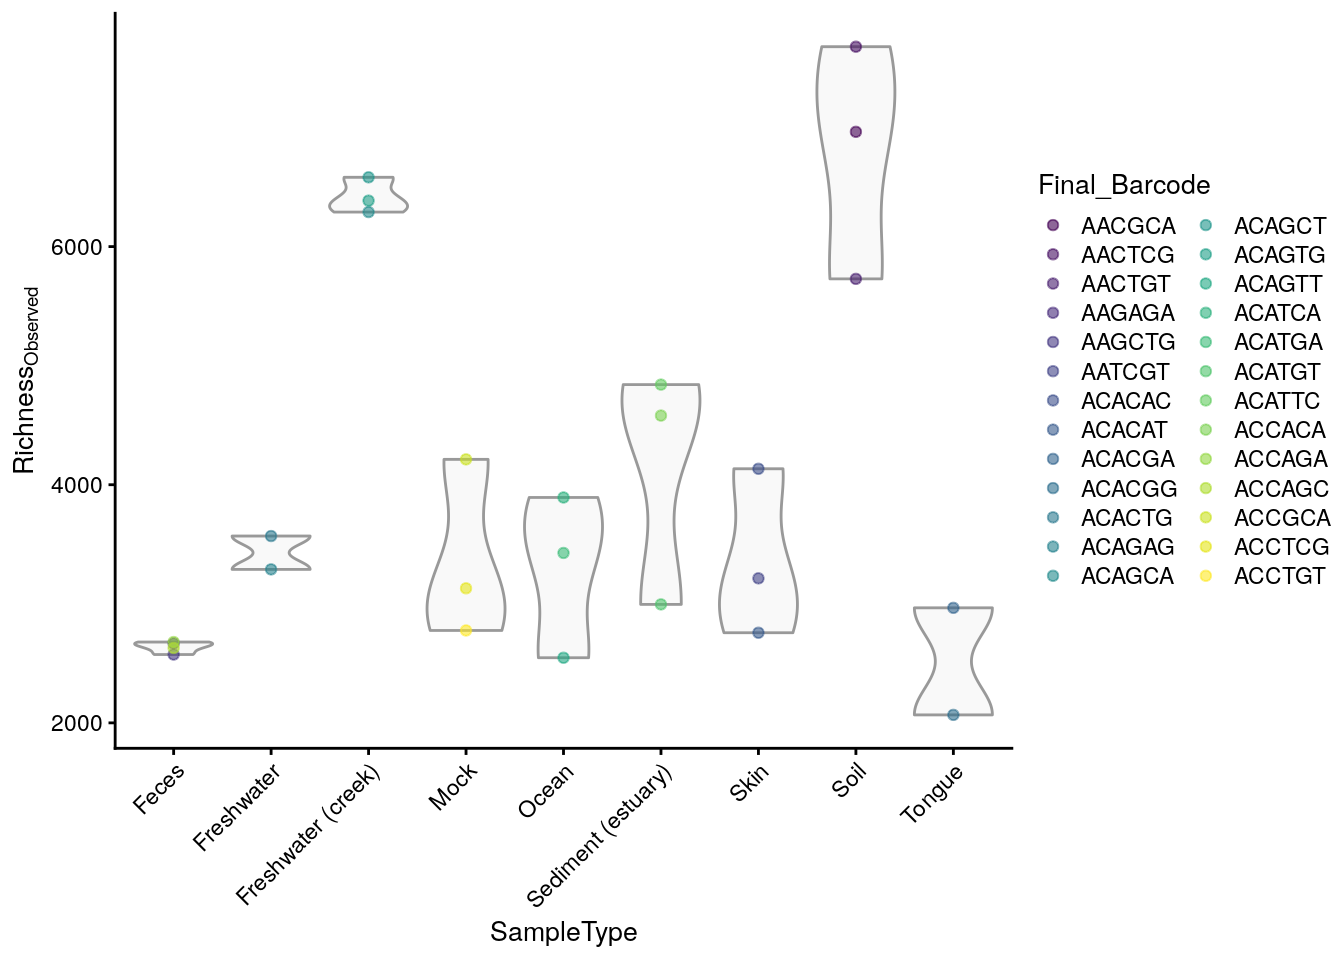
\includegraphics{14_alpha_diversity_files/figure-latex/plot-div-shannon-1.pdf}
\caption{\label{fig:plot-div-shannon}Shannon diversity estimates plotted grouped by sample type with colour-labeled barcode.}
\end{figure}

\hypertarget{diversity}{%
\subsection{Diversity}\label{diversity}}

The main function, \texttt{estimateDiversity}, calculates the selected
diversity index based on the selected assay data.

\begin{Shaded}
\begin{Highlighting}[]
\NormalTok{tse }\OtherTok{\textless{}{-}}\NormalTok{ mia}\SpecialCharTok{::}\FunctionTok{estimateDiversity}\NormalTok{(tse, }
                              \AttributeTok{abund\_values =} \StringTok{"counts"}\NormalTok{,}
                              \AttributeTok{index =} \StringTok{"shannon"}\NormalTok{, }
                              \AttributeTok{name =} \StringTok{"shannon"}\NormalTok{)}
\FunctionTok{head}\NormalTok{(}\FunctionTok{colData}\NormalTok{(tse)}\SpecialCharTok{$}\NormalTok{shannon)}
\end{Highlighting}
\end{Shaded}

\begin{verbatim}
##     CL3     CC1     SV1 M31Fcsw M11Fcsw M31Plmr 
##   6.577   6.777   6.498   3.828   3.288   4.289
\end{verbatim}

Alpha diversities can be visualized with boxplot. Here, Shannon index is compared
between different sample type groups. Individual data points are visualized by
plotting them as points with \texttt{geom\_jitter}.

\texttt{geom\_signif} is used to test whether these differences are statistically significant.
It adds p-values to plot.

\begin{Shaded}
\begin{Highlighting}[]
\ControlFlowTok{if}\NormalTok{( }\SpecialCharTok{!}\FunctionTok{require}\NormalTok{(ggsignif) )\{}
  \FunctionTok{install.packages}\NormalTok{(ggsignif)}
\NormalTok{\}}
\FunctionTok{library}\NormalTok{(ggplot2)}
\FunctionTok{library}\NormalTok{(patchwork)}
\FunctionTok{library}\NormalTok{(ggsignif)}

\CommentTok{\# Subsets the data. Takes only those samples that are from feces, skin, or tongue,}
\CommentTok{\# and creates data frame from the collected data}
\NormalTok{df }\OtherTok{\textless{}{-}} \FunctionTok{as.data.frame}\NormalTok{(}\FunctionTok{colData}\NormalTok{(tse)[}\FunctionTok{colData}\NormalTok{(tse)}\SpecialCharTok{$}\NormalTok{SampleType }\SpecialCharTok{\%in\%} 
                                  \FunctionTok{c}\NormalTok{(}\StringTok{"Feces"}\NormalTok{, }\StringTok{"Skin"}\NormalTok{, }\StringTok{"Tongue"}\NormalTok{), ])}

\CommentTok{\# Changes old levels with new levels}
\NormalTok{df}\SpecialCharTok{$}\NormalTok{SampleType }\OtherTok{\textless{}{-}} \FunctionTok{factor}\NormalTok{(df}\SpecialCharTok{$}\NormalTok{SampleType)}

\CommentTok{\# For significance testing, all different combinations are determined}
\NormalTok{comb }\OtherTok{\textless{}{-}} \FunctionTok{split}\NormalTok{(}\FunctionTok{t}\NormalTok{(}\FunctionTok{combn}\NormalTok{(}\FunctionTok{levels}\NormalTok{(df}\SpecialCharTok{$}\NormalTok{SampleType), }\DecValTok{2}\NormalTok{)), }
           \FunctionTok{seq}\NormalTok{(}\FunctionTok{nrow}\NormalTok{(}\FunctionTok{t}\NormalTok{(}\FunctionTok{combn}\NormalTok{(}\FunctionTok{levels}\NormalTok{(df}\SpecialCharTok{$}\NormalTok{SampleType), }\DecValTok{2}\NormalTok{)))))}

\FunctionTok{ggplot}\NormalTok{(df, }\FunctionTok{aes}\NormalTok{(}\AttributeTok{x =}\NormalTok{ SampleType, }\AttributeTok{y =}\NormalTok{ shannon)) }\SpecialCharTok{+}
  \CommentTok{\# Outliers are removed, because otherwise each data point would be plotted twice; }
  \CommentTok{\# as an outlier of boxplot and as a point of dotplot.}
  \FunctionTok{geom\_boxplot}\NormalTok{(}\AttributeTok{outlier.shape =} \ConstantTok{NA}\NormalTok{) }\SpecialCharTok{+} 
  \FunctionTok{geom\_jitter}\NormalTok{(}\AttributeTok{width =} \FloatTok{0.2}\NormalTok{) }\SpecialCharTok{+} 
  \FunctionTok{geom\_signif}\NormalTok{(}\AttributeTok{comparisons =}\NormalTok{ comb, }\AttributeTok{map\_signif\_level =} \ConstantTok{FALSE}\NormalTok{) }\SpecialCharTok{+}
  \FunctionTok{theme}\NormalTok{(}\AttributeTok{text =} \FunctionTok{element\_text}\NormalTok{(}\AttributeTok{size =} \DecValTok{10}\NormalTok{))}
\end{Highlighting}
\end{Shaded}

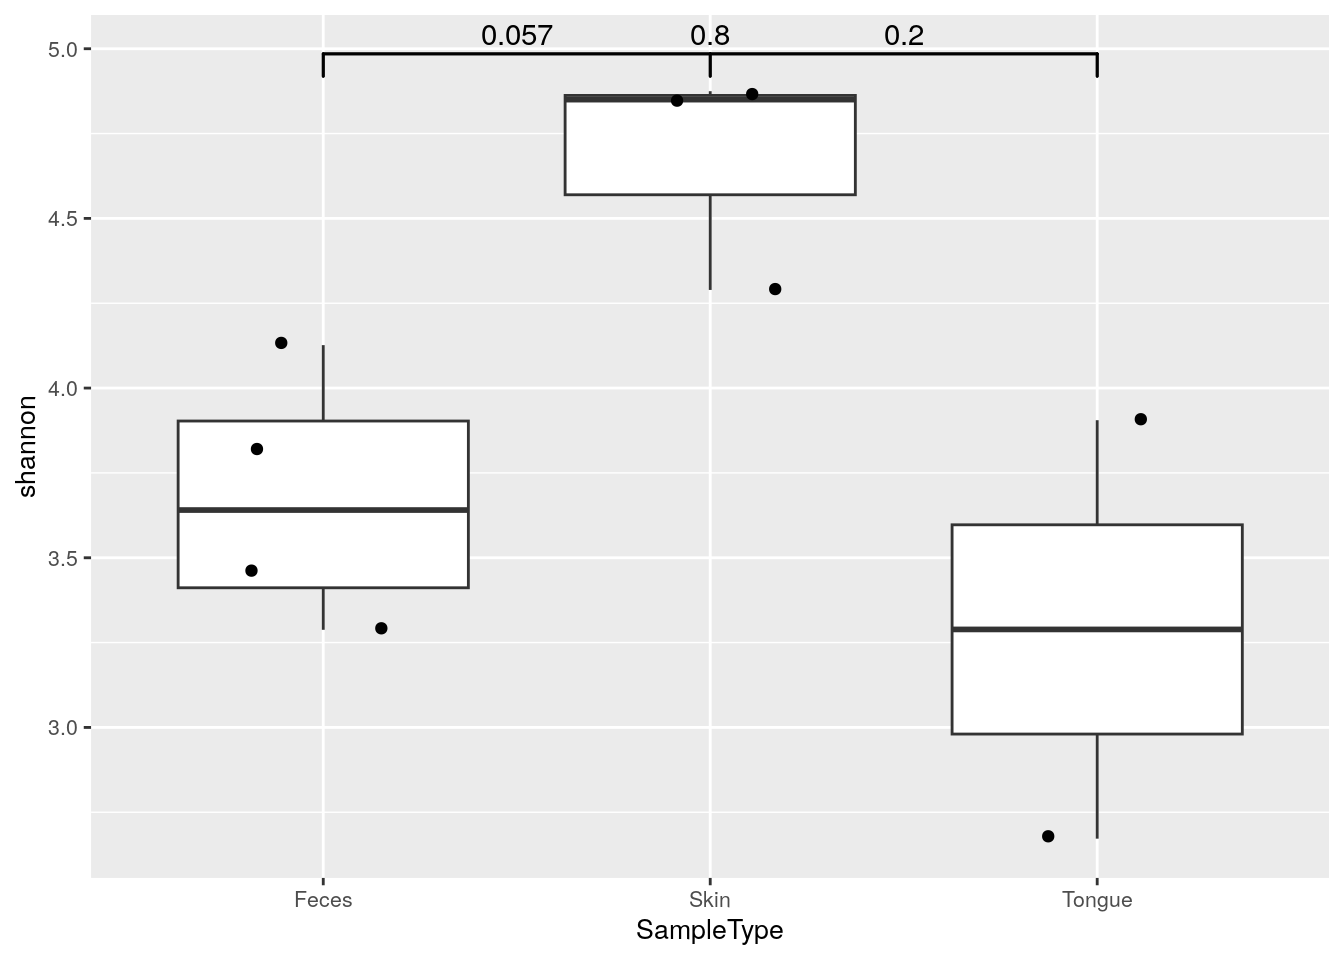
\includegraphics{14_alpha_diversity_files/figure-latex/visualize-shannon-1.pdf}

\hypertarget{faith-phylogenetic-diversity}{%
\subsection{Faith phylogenetic diversity}\label{faith-phylogenetic-diversity}}

The Faith index is returned by the function \texttt{estimateFaith}.

\begin{Shaded}
\begin{Highlighting}[]
\NormalTok{tse }\OtherTok{\textless{}{-}}\NormalTok{ mia}\SpecialCharTok{::}\FunctionTok{estimateFaith}\NormalTok{(tse,}
                          \AttributeTok{abund\_values =} \StringTok{"counts"}\NormalTok{)}
\FunctionTok{head}\NormalTok{(}\FunctionTok{colData}\NormalTok{(tse)}\SpecialCharTok{$}\NormalTok{faith)}
\end{Highlighting}
\end{Shaded}

\begin{verbatim}
## [1] 250.5 262.3 208.5 117.9 119.8 135.8
\end{verbatim}

\textbf{Note}: because \texttt{tse} is a \texttt{TreeSummarizedExperiment} object, its phylogenetic tree is used by default. However, the optional argument \texttt{tree} must be provided if \texttt{tse} does not contain one.

Below a visual comparison between shannon and faith indices is shown with a violin plot.

\begin{Shaded}
\begin{Highlighting}[]
\NormalTok{plots }\OtherTok{\textless{}{-}} \FunctionTok{lapply}\NormalTok{(}\FunctionTok{c}\NormalTok{(}\StringTok{"shannon"}\NormalTok{, }\StringTok{"faith"}\NormalTok{),}
\NormalTok{                plotColData,}
                \AttributeTok{object =}\NormalTok{ tse, }\AttributeTok{colour\_by =} \StringTok{"SampleType"}\NormalTok{)}
\NormalTok{plots[[}\DecValTok{1}\NormalTok{]] }\SpecialCharTok{+}\NormalTok{ plots[[}\DecValTok{2}\NormalTok{]] }\SpecialCharTok{+}
  \FunctionTok{plot\_layout}\NormalTok{(}\AttributeTok{guides =} \StringTok{"collect"}\NormalTok{)}
\end{Highlighting}
\end{Shaded}

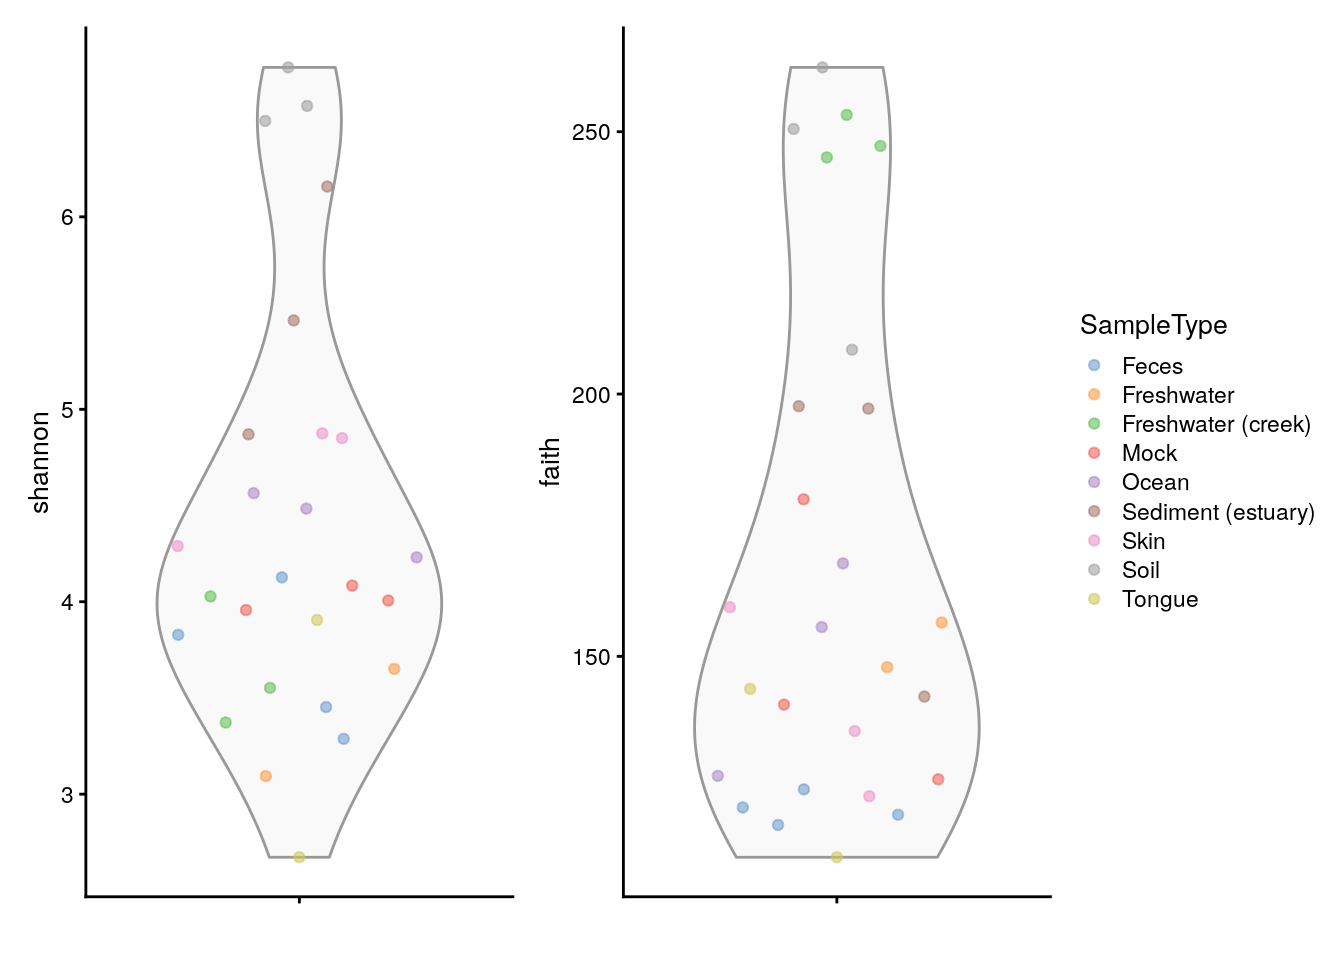
\includegraphics{14_alpha_diversity_files/figure-latex/phylo-div-2-1.pdf}

Alternatively, the phylogenetic diversity can be calculated by \texttt{mia::estimateDiversity}. This is a faster re-implementation of\\
the widely used function in \emph{\texttt{picante}} \citep[\citet{Kembel2010}]{R-picante}.

Load \texttt{picante} R package and get the \texttt{phylo} stored in \texttt{rowTree}.

\begin{Shaded}
\begin{Highlighting}[]
\NormalTok{tse }\OtherTok{\textless{}{-}}\NormalTok{ mia}\SpecialCharTok{::}\FunctionTok{estimateDiversity}\NormalTok{(tse, }
                              \AttributeTok{abund\_values =} \StringTok{"counts"}\NormalTok{,}
                              \AttributeTok{index =} \StringTok{"faith"}\NormalTok{, }
                              \AttributeTok{name =} \StringTok{"faith"}\NormalTok{)}
\end{Highlighting}
\end{Shaded}

\hypertarget{evenness}{%
\subsection{Evenness}\label{evenness}}

Evenness can be calculated with \texttt{estimateEvenness}.

\begin{Shaded}
\begin{Highlighting}[]
\NormalTok{tse }\OtherTok{\textless{}{-}} \FunctionTok{estimateEvenness}\NormalTok{(tse, }
                        \AttributeTok{abund\_values =} \StringTok{"counts"}\NormalTok{, }
                        \AttributeTok{index=}\StringTok{"simpson"}\NormalTok{)}
\FunctionTok{head}\NormalTok{(}\FunctionTok{colData}\NormalTok{(tse)}\SpecialCharTok{$}\NormalTok{simpson)}
\end{Highlighting}
\end{Shaded}

\begin{verbatim}
## [1] 0.026871 0.027197 0.047049 0.005179 0.004304 0.005011
\end{verbatim}

\hypertarget{dominance}{%
\subsection{Dominance}\label{dominance}}

Dominance can be calculated with \texttt{estimateDominance}. Here, the \texttt{Relative\ index} is calculated which is the relative abundance of the most dominant species in the sample.

\begin{Shaded}
\begin{Highlighting}[]
\NormalTok{tse }\OtherTok{\textless{}{-}} \FunctionTok{estimateDominance}\NormalTok{(tse, }
                         \AttributeTok{abund\_values =} \StringTok{"counts"}\NormalTok{, }
                         \AttributeTok{index=}\StringTok{"relative"}\NormalTok{)}

\FunctionTok{head}\NormalTok{(}\FunctionTok{colData}\NormalTok{(tse)}\SpecialCharTok{$}\NormalTok{relative)}
\end{Highlighting}
\end{Shaded}

\begin{verbatim}
##     CL3     CC1     SV1 M31Fcsw M11Fcsw M31Plmr 
## 0.03910 0.03226 0.01690 0.22981 0.21778 0.22329
\end{verbatim}

\hypertarget{rarity}{%
\subsection{Rarity}\label{rarity}}

\texttt{mia} package provides one rarity index called log-modulo skewness. It can be
calculated with \texttt{estimateDiversity}.

\begin{Shaded}
\begin{Highlighting}[]
\NormalTok{tse }\OtherTok{\textless{}{-}}\NormalTok{ mia}\SpecialCharTok{::}\FunctionTok{estimateDiversity}\NormalTok{(tse, }
                              \AttributeTok{abund\_values =} \StringTok{"counts"}\NormalTok{,}
                              \AttributeTok{index =} \StringTok{"log\_modulo\_skewness"}\NormalTok{)}

\FunctionTok{head}\NormalTok{(}\FunctionTok{colData}\NormalTok{(tse)}\SpecialCharTok{$}\NormalTok{log\_modulo\_skewness)}
\end{Highlighting}
\end{Shaded}

\begin{verbatim}
## [1] 2.061 2.061 2.061 2.061 2.061 2.061
\end{verbatim}

\hypertarget{divergence}{%
\subsection{Divergence}\label{divergence}}

Divergence can be evaluated with \texttt{estimateDivergence}. Reference and algorithm for the calculation of divergence can be specified as \texttt{reference} and \texttt{FUN}, respectively.

\begin{Shaded}
\begin{Highlighting}[]
\NormalTok{tse }\OtherTok{\textless{}{-}}\NormalTok{ mia}\SpecialCharTok{::}\FunctionTok{estimateDivergence}\NormalTok{(tse,}
                               \AttributeTok{abund\_values =} \StringTok{"counts"}\NormalTok{,}
                               \AttributeTok{reference =} \StringTok{"median"}\NormalTok{,}
                               \AttributeTok{FUN =}\NormalTok{ vegan}\SpecialCharTok{::}\NormalTok{vegdist)}
\end{Highlighting}
\end{Shaded}

\hypertarget{visualization}{%
\section{Visualization}\label{visualization}}

A plot comparing all the diversity measures calculated above and stored in \texttt{colData} can then be constructed directly.

\begin{Shaded}
\begin{Highlighting}[]
\NormalTok{plots }\OtherTok{\textless{}{-}} \FunctionTok{lapply}\NormalTok{(}\FunctionTok{c}\NormalTok{(}\StringTok{"observed"}\NormalTok{, }\StringTok{"shannon"}\NormalTok{, }\StringTok{"simpson"}\NormalTok{, }\StringTok{"relative"}\NormalTok{, }\StringTok{"faith"}\NormalTok{, }\StringTok{"log\_modulo\_skewness"}\NormalTok{),}
\NormalTok{                plotColData,}
                \AttributeTok{object =}\NormalTok{ tse,}
                \AttributeTok{x =} \StringTok{"SampleType"}\NormalTok{,}
                \AttributeTok{colour\_by =} \StringTok{"SampleType"}\NormalTok{)}

\NormalTok{plots }\OtherTok{\textless{}{-}} \FunctionTok{lapply}\NormalTok{(plots, }\StringTok{"+"}\NormalTok{, }
                \FunctionTok{theme}\NormalTok{(}\AttributeTok{axis.text.x =} \FunctionTok{element\_blank}\NormalTok{(),}
                      \AttributeTok{axis.title.x =} \FunctionTok{element\_blank}\NormalTok{(),}
                      \AttributeTok{axis.ticks.x =} \FunctionTok{element\_blank}\NormalTok{()))}

\NormalTok{((plots[[}\DecValTok{1}\NormalTok{]] }\SpecialCharTok{|}\NormalTok{ plots[[}\DecValTok{2}\NormalTok{]] }\SpecialCharTok{|}\NormalTok{ plots[[}\DecValTok{3}\NormalTok{]]) }\SpecialCharTok{/} 
\NormalTok{(plots[[}\DecValTok{4}\NormalTok{]] }\SpecialCharTok{|}\NormalTok{ plots[[}\DecValTok{5}\NormalTok{]] }\SpecialCharTok{|}\NormalTok{ plots[[}\DecValTok{6}\NormalTok{]])) }\SpecialCharTok{+}
  \FunctionTok{plot\_layout}\NormalTok{(}\AttributeTok{guides =} \StringTok{"collect"}\NormalTok{)}
\end{Highlighting}
\end{Shaded}

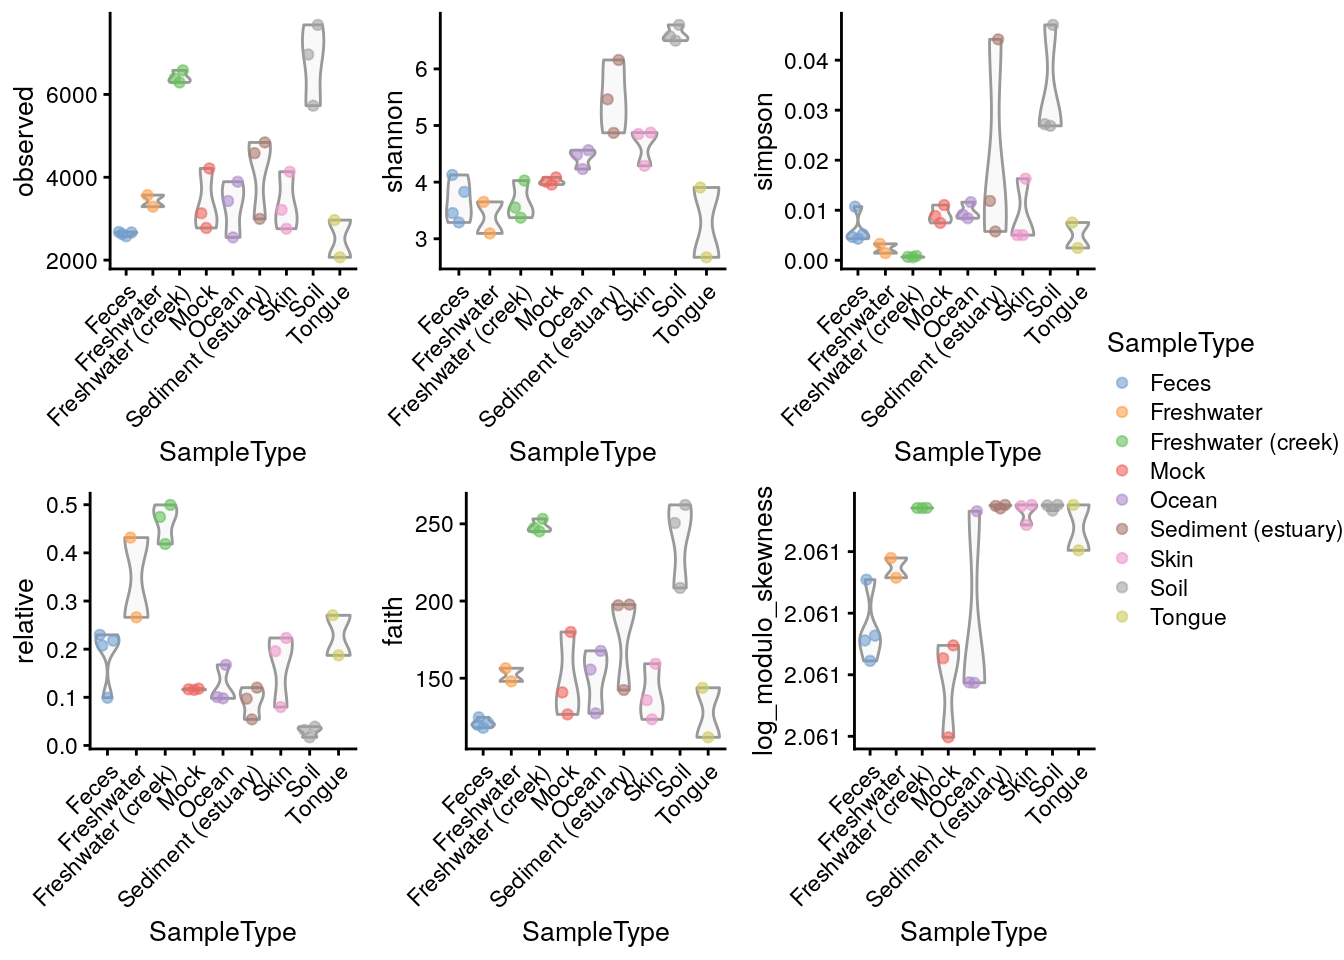
\includegraphics{14_alpha_diversity_files/figure-latex/plot-all-diversities-1.pdf}

\hypertarget{session-info-4}{%
\section*{Session Info}\label{session-info-4}}
\addcontentsline{toc}{section}{Session Info}

View session info

\begin{verbatim}
R version 4.1.2 (2021-11-01)
Platform: x86_64-pc-linux-gnu (64-bit)
Running under: Ubuntu 20.04.3 LTS

Matrix products: default
BLAS/LAPACK: /usr/lib/x86_64-linux-gnu/openblas-pthread/libopenblasp-r0.3.8.so

locale:
 [1] LC_CTYPE=en_US.UTF-8       LC_NUMERIC=C              
 [3] LC_TIME=en_US.UTF-8        LC_COLLATE=en_US.UTF-8    
 [5] LC_MONETARY=en_US.UTF-8    LC_MESSAGES=en_US.UTF-8   
 [7] LC_PAPER=en_US.UTF-8       LC_NAME=C                 
 [9] LC_ADDRESS=C               LC_TELEPHONE=C            
[11] LC_MEASUREMENT=en_US.UTF-8 LC_IDENTIFICATION=C       

attached base packages:
[1] stats4    stats     graphics  grDevices utils     datasets  methods  
[8] base     

other attached packages:
 [1] patchwork_1.1.1                ggsignif_0.6.3                
 [3] scater_1.22.0                  ggplot2_3.3.5                 
 [5] scuttle_1.4.0                  mia_1.3.19                    
 [7] MultiAssayExperiment_1.20.0    TreeSummarizedExperiment_2.1.4
 [9] Biostrings_2.62.0              XVector_0.34.0                
[11] SingleCellExperiment_1.16.0    SummarizedExperiment_1.24.0   
[13] Biobase_2.54.0                 GenomicRanges_1.46.1          
[15] GenomeInfoDb_1.30.1            IRanges_2.28.0                
[17] S4Vectors_0.32.3               BiocGenerics_0.40.0           
[19] MatrixGenerics_1.6.0           matrixStats_0.61.0-9001       
[21] BiocStyle_2.22.0               rebook_1.4.0                  

loaded via a namespace (and not attached):
  [1] ggbeeswarm_0.6.0            colorspace_2.0-3           
  [3] ellipsis_0.3.2              BiocNeighbors_1.12.0       
  [5] farver_2.1.0                ggrepel_0.9.1              
  [7] bit64_4.0.5                 fansi_1.0.2                
  [9] decontam_1.14.0             splines_4.1.2              
 [11] codetools_0.2-18            sparseMatrixStats_1.6.0    
 [13] cachem_1.0.6                knitr_1.37                 
 [15] jsonlite_1.8.0              cluster_2.1.2              
 [17] graph_1.72.0                BiocManager_1.30.16        
 [19] compiler_4.1.2              assertthat_0.2.1           
 [21] Matrix_1.4-0                fastmap_1.1.0              
 [23] lazyeval_0.2.2              cli_3.2.0                  
 [25] BiocSingular_1.10.0         htmltools_0.5.2            
 [27] tools_4.1.2                 rsvd_1.0.5                 
 [29] gtable_0.3.0                glue_1.6.2                 
 [31] GenomeInfoDbData_1.2.7      reshape2_1.4.4             
 [33] dplyr_1.0.8                 Rcpp_1.0.8.3               
 [35] vctrs_0.3.8                 ape_5.6-2                  
 [37] nlme_3.1-155                DECIPHER_2.22.0            
 [39] DelayedMatrixStats_1.16.0   xfun_0.30                  
 [41] stringr_1.4.0               beachmat_2.10.0            
 [43] lifecycle_1.0.1             irlba_2.3.5                
 [45] XML_3.99-0.9                zlibbioc_1.40.0            
 [47] MASS_7.3-55                 scales_1.1.1               
 [49] parallel_4.1.2              yaml_2.3.5                 
 [51] memoise_2.0.1               gridExtra_2.3              
 [53] yulab.utils_0.0.4           stringi_1.7.6              
 [55] RSQLite_2.2.10              highr_0.9                  
 [57] ScaledMatrix_1.2.0          tidytree_0.3.9             
 [59] permute_0.9-7               filelock_1.0.2             
 [61] BiocParallel_1.28.3         rlang_1.0.2                
 [63] pkgconfig_2.0.3             bitops_1.0-7               
 [65] evaluate_0.15               lattice_0.20-45            
 [67] purrr_0.3.4                 labeling_0.4.2             
 [69] treeio_1.18.1               CodeDepends_0.6.5          
 [71] cowplot_1.1.1               bit_4.0.4                  
 [73] tidyselect_1.1.2            plyr_1.8.6                 
 [75] magrittr_2.0.2              bookdown_0.25              
 [77] R6_2.5.1                    generics_0.1.2             
 [79] DelayedArray_0.20.0         DBI_1.1.2                  
 [81] withr_2.5.0                 mgcv_1.8-39                
 [83] pillar_1.7.0                RCurl_1.98-1.6             
 [85] tibble_3.1.6                dir.expiry_1.2.0           
 [87] crayon_1.5.0                utf8_1.2.2                 
 [89] rmarkdown_2.13              viridis_0.6.2              
 [91] grid_4.1.2                  blob_1.2.2                 
 [93] vegan_2.5-7                 digest_0.6.29              
 [95] tidyr_1.2.0                 munsell_0.5.0              
 [97] DirichletMultinomial_1.36.0 beeswarm_0.4.0             
 [99] viridisLite_0.4.0           vipor_0.4.5                
\end{verbatim}

\hypertarget{community-similarity}{%
\chapter{Community similarity}\label{community-similarity}}

Where alpha diversity focuses on community variation within a
community (sample), beta diversity quantifies (dis-)similarites
between communities (samples). Some of the most popular beta diversity
measures in microbiome research include Bray-Curtis index (for
compositional data), Jaccard index (for presence / absence data,
ignoring abundance information), Aitchison distance (Euclidean
distance for clr transformed abundances, aiming to avoid the
compositionality bias), and the Unifrac distances (that take into
account the phylogenetic tree information). Only some of the commonly
used beta diversity measures are actual \emph{distances}; this is a
mathematically well-defined concept and many ecological beta diversity
measures, such as Bray-Curtis index, are not proper distances.
Therefore, the term dissimilarity or beta diversity is commonly used.

Technically, beta diversities are usually represented as \texttt{dist}
objects, which contain triangular data describing the distance between
each pair of samples. These distances can be further subjected to
ordination. Ordination is a common concept in ecology that aims to
reduce the dimensionality of the data for further evaluation or
visualization. Ordination techniques aim to capture as much of
essential information in the data as possible in a lower dimensional
representation. Dimension reduction is bound to loose information but
the common ordination techniques aim to preserve relevant information
of sample similarities in an optimal way, which is defined in
different ways by different methods. {[}TODO add references and/or link
to ordination chapter instead?{]}

Some of the most common ordination methods in microbiome research
include Principal Component Analysis (PCA), metric and non-metric
multi-dimensional scaling (MDS, NMDS), The MDS methods are also known
as Principal Coordinates Analysis (PCoA). Other recently popular
techniques include t-SNE and UMAP.

\hypertarget{explained-variance}{%
\section{Explained variance}\label{explained-variance}}

The percentage of explained variance is typically shown for PCA
ordination plots. This quantifies the proportion of overall variance
in the data that is captured by the PCA axes, or how well the
ordination axes reflect the original distances.

Sometimes a similar measure is shown for MDS/PCoA. The interpretation
is generally different, however, and hence we do not recommend using
it. PCA is a special case of PCoA with Euclidean distances. With
non-Euclidean dissimilarities PCoA uses a trick where the pointwise
dissimilarities are first cast into similarities in a Euclidean space
(with some information loss i.e.~stress) and then projected to the
maximal variance axes. In this case, the maximal variance axes do not
directly reflect the correspondence of the projected distances and
original distances, as they do for PCA.

In typical use cases, we would like to know how well the ordination
reflects the original similarity structures; then the quantity of
interest is the so-called ``stress'' function, which measures the
difference in pairwise similarities between the data points in the
original (high-dimensional) vs.~projected (low-dimensional) space.

Hence, we propose that for PCoA and other ordination methods, users
would report relative stress (varies in the unit interval; the smaller
the better). This can be calculated as shown below. For further
examples, check the \href{https://www.huber.embl.de/users/klaus/Teaching/statisticalMethods-lab.pdf}{note from Huber
lab}.

\begin{Shaded}
\begin{Highlighting}[]
\CommentTok{\# Example data}
\FunctionTok{library}\NormalTok{(mia)}
\FunctionTok{data}\NormalTok{(GlobalPatterns, }\AttributeTok{package=}\StringTok{"mia"}\NormalTok{)}

\CommentTok{\# Data matrix (features x samples)}
\NormalTok{tse }\OtherTok{\textless{}{-}}\NormalTok{ GlobalPatterns}
\NormalTok{tse }\OtherTok{\textless{}{-}} \FunctionTok{transformCounts}\NormalTok{(tse, }\AttributeTok{method =} \StringTok{"relabundance"}\NormalTok{)}

\CommentTok{\# Add group information Feces yes/no}
\FunctionTok{colData}\NormalTok{(tse)}\SpecialCharTok{$}\NormalTok{Group }\OtherTok{\textless{}{-}} \FunctionTok{colData}\NormalTok{(tse)}\SpecialCharTok{$}\NormalTok{SampleType}\SpecialCharTok{==}\StringTok{"Feces"}

\CommentTok{\# Quantify dissimilarities in the original feature space}
\FunctionTok{library}\NormalTok{(vegan)}
\NormalTok{x }\OtherTok{\textless{}{-}} \FunctionTok{assay}\NormalTok{(tse, }\StringTok{"relabundance"}\NormalTok{) }\CommentTok{\# Pick relabunance assay separately}
\NormalTok{d0 }\OtherTok{\textless{}{-}} \FunctionTok{as.matrix}\NormalTok{(}\FunctionTok{vegdist}\NormalTok{(}\FunctionTok{t}\NormalTok{(x), }\StringTok{"bray"}\NormalTok{))}

\CommentTok{\# PCoA Ordination}
\NormalTok{pcoa }\OtherTok{\textless{}{-}} \FunctionTok{as.data.frame}\NormalTok{(}\FunctionTok{cmdscale}\NormalTok{(d0, }\AttributeTok{k =} \DecValTok{2}\NormalTok{))}
\FunctionTok{names}\NormalTok{(pcoa) }\OtherTok{\textless{}{-}} \FunctionTok{c}\NormalTok{(}\StringTok{"PCoA1"}\NormalTok{, }\StringTok{"PCoA2"}\NormalTok{)}

\CommentTok{\# Quantify dissimilarities in the ordination space}
\NormalTok{dp }\OtherTok{\textless{}{-}} \FunctionTok{as.matrix}\NormalTok{(}\FunctionTok{dist}\NormalTok{(pcoa))}

\CommentTok{\# Calculate stress i.e. relative difference in the original and}
\CommentTok{\# projected dissimilarities}
\NormalTok{stress }\OtherTok{\textless{}{-}} \FunctionTok{sum}\NormalTok{((dp }\SpecialCharTok{{-}}\NormalTok{ d0)}\SpecialCharTok{\^{}}\DecValTok{2}\NormalTok{)}\SpecialCharTok{/}\FunctionTok{sum}\NormalTok{(d0}\SpecialCharTok{\^{}}\DecValTok{2}\NormalTok{)}
\end{Highlighting}
\end{Shaded}

Shepard plot visualizes the original versus projected (ordination)
dissimilarities between the data points:

\begin{Shaded}
\begin{Highlighting}[]
\NormalTok{ord }\OtherTok{\textless{}{-}} \FunctionTok{order}\NormalTok{(}\FunctionTok{as.vector}\NormalTok{(d0))}
\NormalTok{df }\OtherTok{\textless{}{-}} \FunctionTok{data.frame}\NormalTok{(}\AttributeTok{d0 =} \FunctionTok{as.vector}\NormalTok{(d0)[ord],}
                  \AttributeTok{dmds =} \FunctionTok{as.vector}\NormalTok{(dp)[ord])}

\FunctionTok{library}\NormalTok{(ggplot2)}
\FunctionTok{ggplot}\NormalTok{(}\FunctionTok{aes}\NormalTok{(}\AttributeTok{x =}\NormalTok{ d0, }\AttributeTok{y =}\NormalTok{ dmds), }\AttributeTok{data=}\NormalTok{df) }\SpecialCharTok{+} 
       \FunctionTok{geom\_smooth}\NormalTok{() }\SpecialCharTok{+}
       \FunctionTok{geom\_point}\NormalTok{() }\SpecialCharTok{+}       
       \FunctionTok{labs}\NormalTok{(}\AttributeTok{title =} \StringTok{"Shepard plot"}\NormalTok{,}
       \AttributeTok{x =} \StringTok{"Original distance"}\NormalTok{,}
       \AttributeTok{y =} \StringTok{"MDS distance"}\NormalTok{,       }
            \AttributeTok{subtitle =} \FunctionTok{paste}\NormalTok{(}\StringTok{"Stress:"}\NormalTok{, }\FunctionTok{round}\NormalTok{(stress, }\DecValTok{2}\NormalTok{))) }\SpecialCharTok{+}
  \FunctionTok{theme\_bw}\NormalTok{()}
\end{Highlighting}
\end{Shaded}

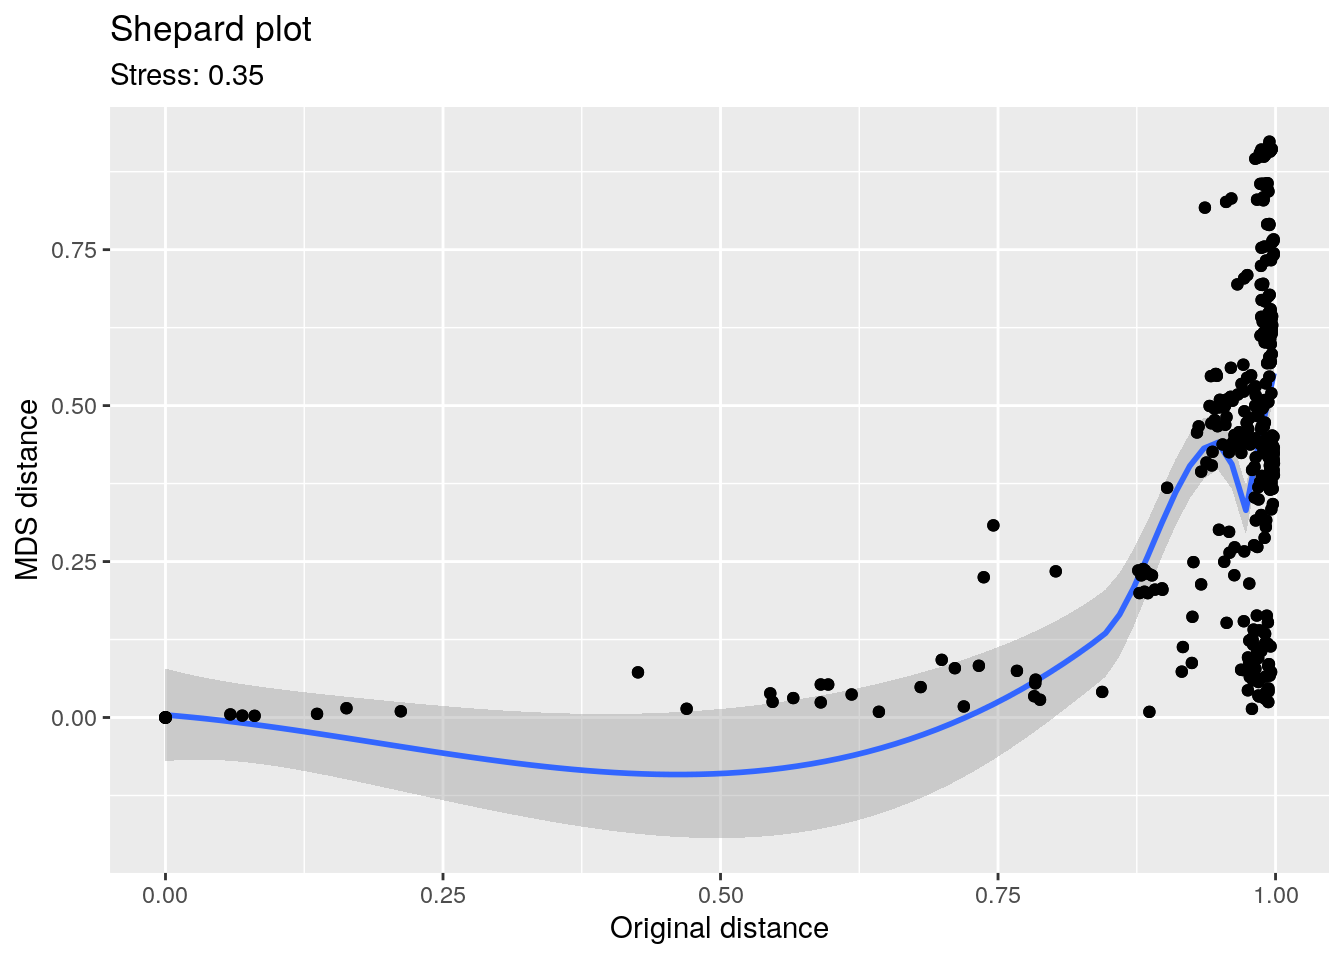
\includegraphics{20_beta_diversity_files/figure-latex/shepard-1.png}

\hypertarget{community-comparisons-by-beta-diversity-analysis}{%
\section{Community comparisons by beta diversity analysis}\label{community-comparisons-by-beta-diversity-analysis}}

A typical comparison of community composition starts with a visual
comparison of the groups on a 2D ordination.

Then we estimate relative abundances and MDS ordination based on
Bray-Curtis (BC) dissimilarity between the groups, and visualize the
results.

In the following examples dissimilarities are calculated by
functions supplied to the \texttt{FUN} argument. This function can be defined by
the user. It must return a \texttt{dist} function, which can then be used to
calculate reduced dimensions either via ordination methods (such as MDS
or NMDS), and the results can be stored in the \texttt{reducedDim}.

This entire process is wrapped in the \texttt{runMDS} and \texttt{runNMDS}
functions.

\begin{Shaded}
\begin{Highlighting}[]
\FunctionTok{library}\NormalTok{(scater)}
\NormalTok{tse }\OtherTok{\textless{}{-}} \FunctionTok{runMDS}\NormalTok{(tse, }\AttributeTok{FUN =}\NormalTok{ vegan}\SpecialCharTok{::}\NormalTok{vegdist, }\AttributeTok{name =} \StringTok{"PCoA\_BC"}\NormalTok{, }\AttributeTok{exprs\_values =} \StringTok{"counts"}\NormalTok{)}
\end{Highlighting}
\end{Shaded}

Sample similarities can be visualized on a lower-dimensional display
(typically 2D) using the \texttt{plotReducedDim} function in the \texttt{scater}
package. This provides also further tools to incorporate additional
information using variations in color, shape or size. Are there
visible differences between the groups?

\begin{Shaded}
\begin{Highlighting}[]
\CommentTok{\# Create ggplot object}
\NormalTok{p }\OtherTok{\textless{}{-}} \FunctionTok{plotReducedDim}\NormalTok{(tse, }\StringTok{"PCoA\_BC"}\NormalTok{, }\AttributeTok{colour\_by =} \StringTok{"Group"}\NormalTok{)}

\CommentTok{\# Add explained variance for each axis}
\NormalTok{e }\OtherTok{\textless{}{-}} \FunctionTok{attr}\NormalTok{(}\FunctionTok{reducedDim}\NormalTok{(tse, }\StringTok{"PCoA\_BC"}\NormalTok{), }\StringTok{"eig"}\NormalTok{);}
\NormalTok{rel\_eig }\OtherTok{\textless{}{-}}\NormalTok{ e}\SpecialCharTok{/}\FunctionTok{sum}\NormalTok{(e[e}\SpecialCharTok{\textgreater{}}\DecValTok{0}\NormalTok{])          }
\NormalTok{p }\OtherTok{\textless{}{-}}\NormalTok{ p }\SpecialCharTok{+} \FunctionTok{labs}\NormalTok{(}\AttributeTok{x =} \FunctionTok{paste}\NormalTok{(}\StringTok{"PCoA 1 ("}\NormalTok{, }\FunctionTok{round}\NormalTok{(}\DecValTok{100} \SpecialCharTok{*}\NormalTok{ rel\_eig[[}\DecValTok{1}\NormalTok{]],}\DecValTok{1}\NormalTok{), }\StringTok{"\%"}\NormalTok{, }\StringTok{")"}\NormalTok{, }\AttributeTok{sep =} \StringTok{""}\NormalTok{),}
              \AttributeTok{y =} \FunctionTok{paste}\NormalTok{(}\StringTok{"PCoA 2 ("}\NormalTok{, }\FunctionTok{round}\NormalTok{(}\DecValTok{100} \SpecialCharTok{*}\NormalTok{ rel\_eig[[}\DecValTok{2}\NormalTok{]],}\DecValTok{1}\NormalTok{), }\StringTok{"\%"}\NormalTok{, }\StringTok{")"}\NormalTok{, }\AttributeTok{sep =} \StringTok{""}\NormalTok{))}

\FunctionTok{print}\NormalTok{(p)}
\end{Highlighting}
\end{Shaded}

\begin{figure}
\centering
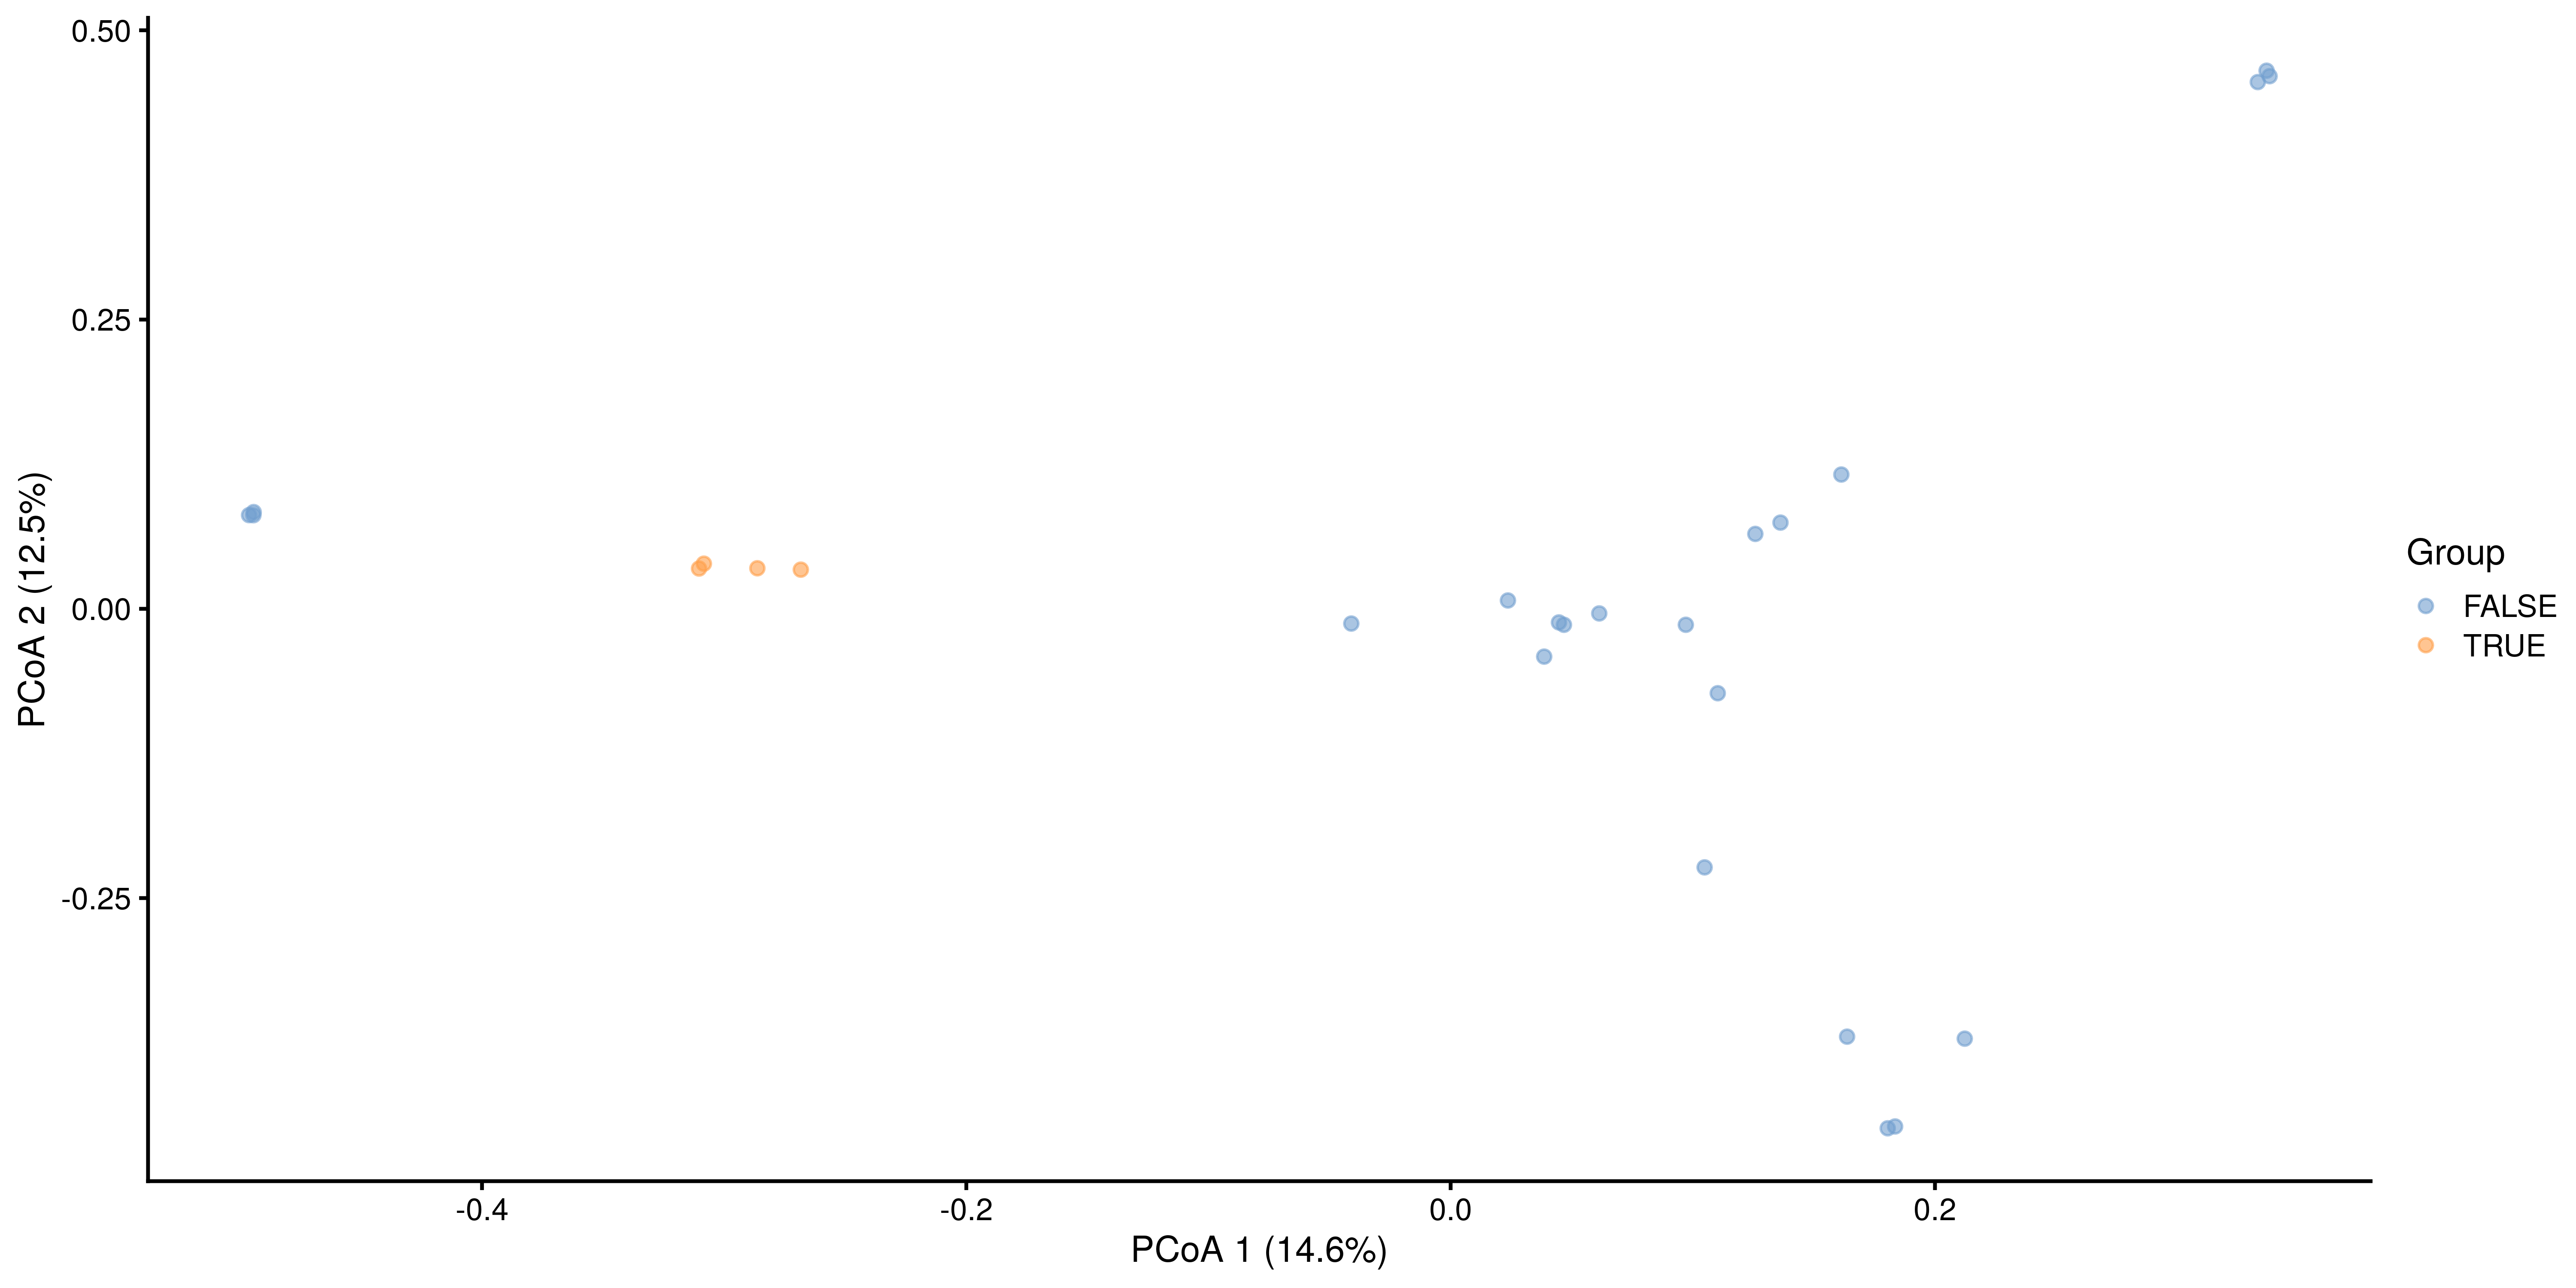
\includegraphics{20_beta_diversity_files/figure-latex/plot-mds-bray-curtis-1.png}
\caption{\label{fig:plot-mds-bray-curtis}MDS plot based on the Bray-Curtis distances on the GlobalPattern dataset.}
\end{figure}

With additional tools from the \texttt{ggplot2} universe, comparisons can be
performed informing on the applicability to visualize sample similarities in a
meaningful way.

\begin{Shaded}
\begin{Highlighting}[]
\NormalTok{tse }\OtherTok{\textless{}{-}} \FunctionTok{runMDS}\NormalTok{(tse, }\AttributeTok{FUN =}\NormalTok{ vegan}\SpecialCharTok{::}\NormalTok{vegdist, }\AttributeTok{name =} \StringTok{"MDS\_euclidean"}\NormalTok{,}
             \AttributeTok{method =} \StringTok{"euclidean"}\NormalTok{, }\AttributeTok{exprs\_values =} \StringTok{"counts"}\NormalTok{)}
\NormalTok{tse }\OtherTok{\textless{}{-}} \FunctionTok{runNMDS}\NormalTok{(tse, }\AttributeTok{FUN =}\NormalTok{ vegan}\SpecialCharTok{::}\NormalTok{vegdist, }\AttributeTok{name =} \StringTok{"NMDS\_BC"}\NormalTok{)}
\end{Highlighting}
\end{Shaded}

\begin{verbatim}
## initial  value 47.733208 
## iter   5 value 33.853364
## iter  10 value 32.891200
## final  value 32.823570 
## converged
\end{verbatim}

\begin{Shaded}
\begin{Highlighting}[]
\NormalTok{tse }\OtherTok{\textless{}{-}} \FunctionTok{runNMDS}\NormalTok{(tse, }\AttributeTok{FUN =}\NormalTok{ vegan}\SpecialCharTok{::}\NormalTok{vegdist, }\AttributeTok{name =} \StringTok{"NMDS\_euclidean"}\NormalTok{,}
               \AttributeTok{method =} \StringTok{"euclidean"}\NormalTok{)}
\end{Highlighting}
\end{Shaded}

\begin{verbatim}
## initial  value 31.882673 
## final  value 31.882673 
## converged
\end{verbatim}

\begin{Shaded}
\begin{Highlighting}[]
\NormalTok{plots }\OtherTok{\textless{}{-}} \FunctionTok{lapply}\NormalTok{(}\FunctionTok{c}\NormalTok{(}\StringTok{"PCoA\_BC"}\NormalTok{, }\StringTok{"MDS\_euclidean"}\NormalTok{, }\StringTok{"NMDS\_BC"}\NormalTok{, }\StringTok{"NMDS\_euclidean"}\NormalTok{),}
\NormalTok{                plotReducedDim,}
                \AttributeTok{object =}\NormalTok{ tse,}
                \AttributeTok{colour\_by =} \StringTok{"Group"}\NormalTok{)}

\FunctionTok{library}\NormalTok{(patchwork)}
\NormalTok{plots[[}\DecValTok{1}\NormalTok{]] }\SpecialCharTok{+}\NormalTok{ plots[[}\DecValTok{2}\NormalTok{]] }\SpecialCharTok{+}\NormalTok{ plots[[}\DecValTok{3}\NormalTok{]] }\SpecialCharTok{+}\NormalTok{ plots[[}\DecValTok{4}\NormalTok{]] }\SpecialCharTok{+}
  \FunctionTok{plot\_layout}\NormalTok{(}\AttributeTok{guides =} \StringTok{"collect"}\NormalTok{)}
\end{Highlighting}
\end{Shaded}

\begin{figure}
\centering
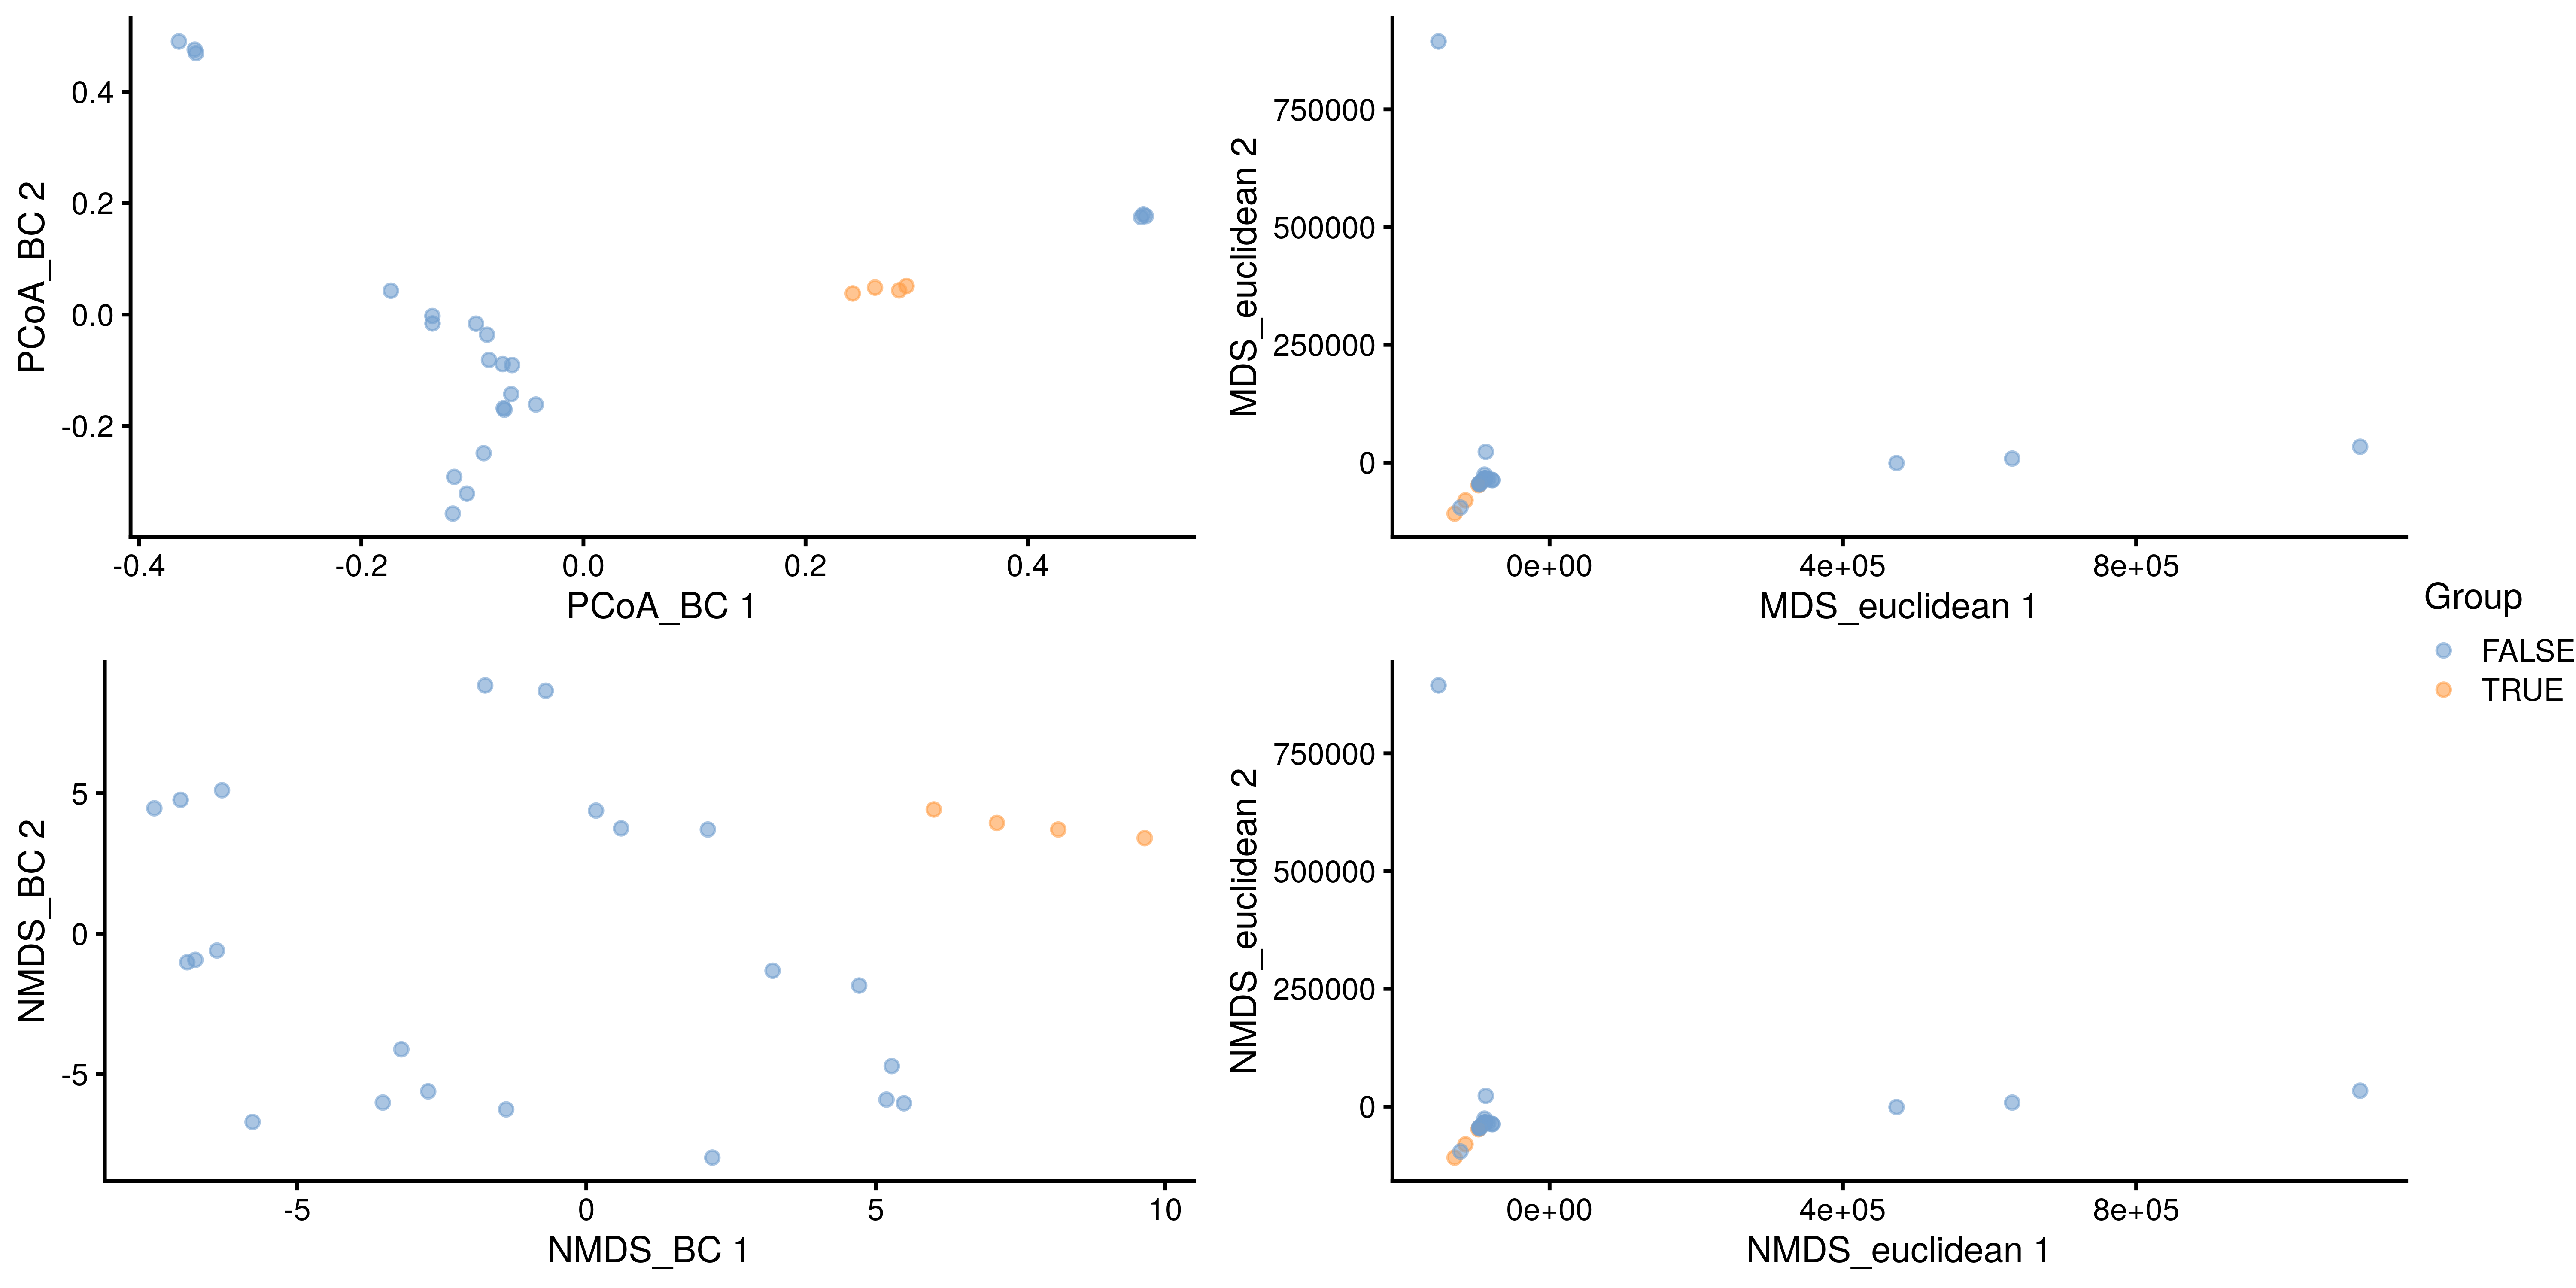
\includegraphics{20_beta_diversity_files/figure-latex/plot-mds-nmds-comparison-1.png}
\caption{\label{fig:plot-mds-nmds-comparison}Comparison of MDS and NMDS plots based on the Bray-Curtis or euclidean distances on the GlobalPattern dataset.}
\end{figure}

The \emph{Unifrac} method is a special case, as it requires data on the
relationship of features in form on a \texttt{phylo} tree. \texttt{calculateUnifrac}
performs the calculation to return a \texttt{dist} object, which can again be
used within \texttt{runMDS}.

\begin{Shaded}
\begin{Highlighting}[]
\FunctionTok{library}\NormalTok{(scater)}
\NormalTok{tse }\OtherTok{\textless{}{-}} \FunctionTok{runMDS}\NormalTok{(tse, }\AttributeTok{FUN =}\NormalTok{ mia}\SpecialCharTok{::}\NormalTok{calculateUnifrac, }\AttributeTok{name =} \StringTok{"Unifrac"}\NormalTok{,}
              \AttributeTok{tree =} \FunctionTok{rowTree}\NormalTok{(tse),}
              \AttributeTok{ntop =} \FunctionTok{nrow}\NormalTok{(tse),}
             \AttributeTok{exprs\_values =} \StringTok{"counts"}\NormalTok{)}
\end{Highlighting}
\end{Shaded}

\begin{Shaded}
\begin{Highlighting}[]
\FunctionTok{plotReducedDim}\NormalTok{(tse, }\StringTok{"Unifrac"}\NormalTok{, }\AttributeTok{colour\_by =} \StringTok{"Group"}\NormalTok{)}
\end{Highlighting}
\end{Shaded}

\begin{figure}
\centering
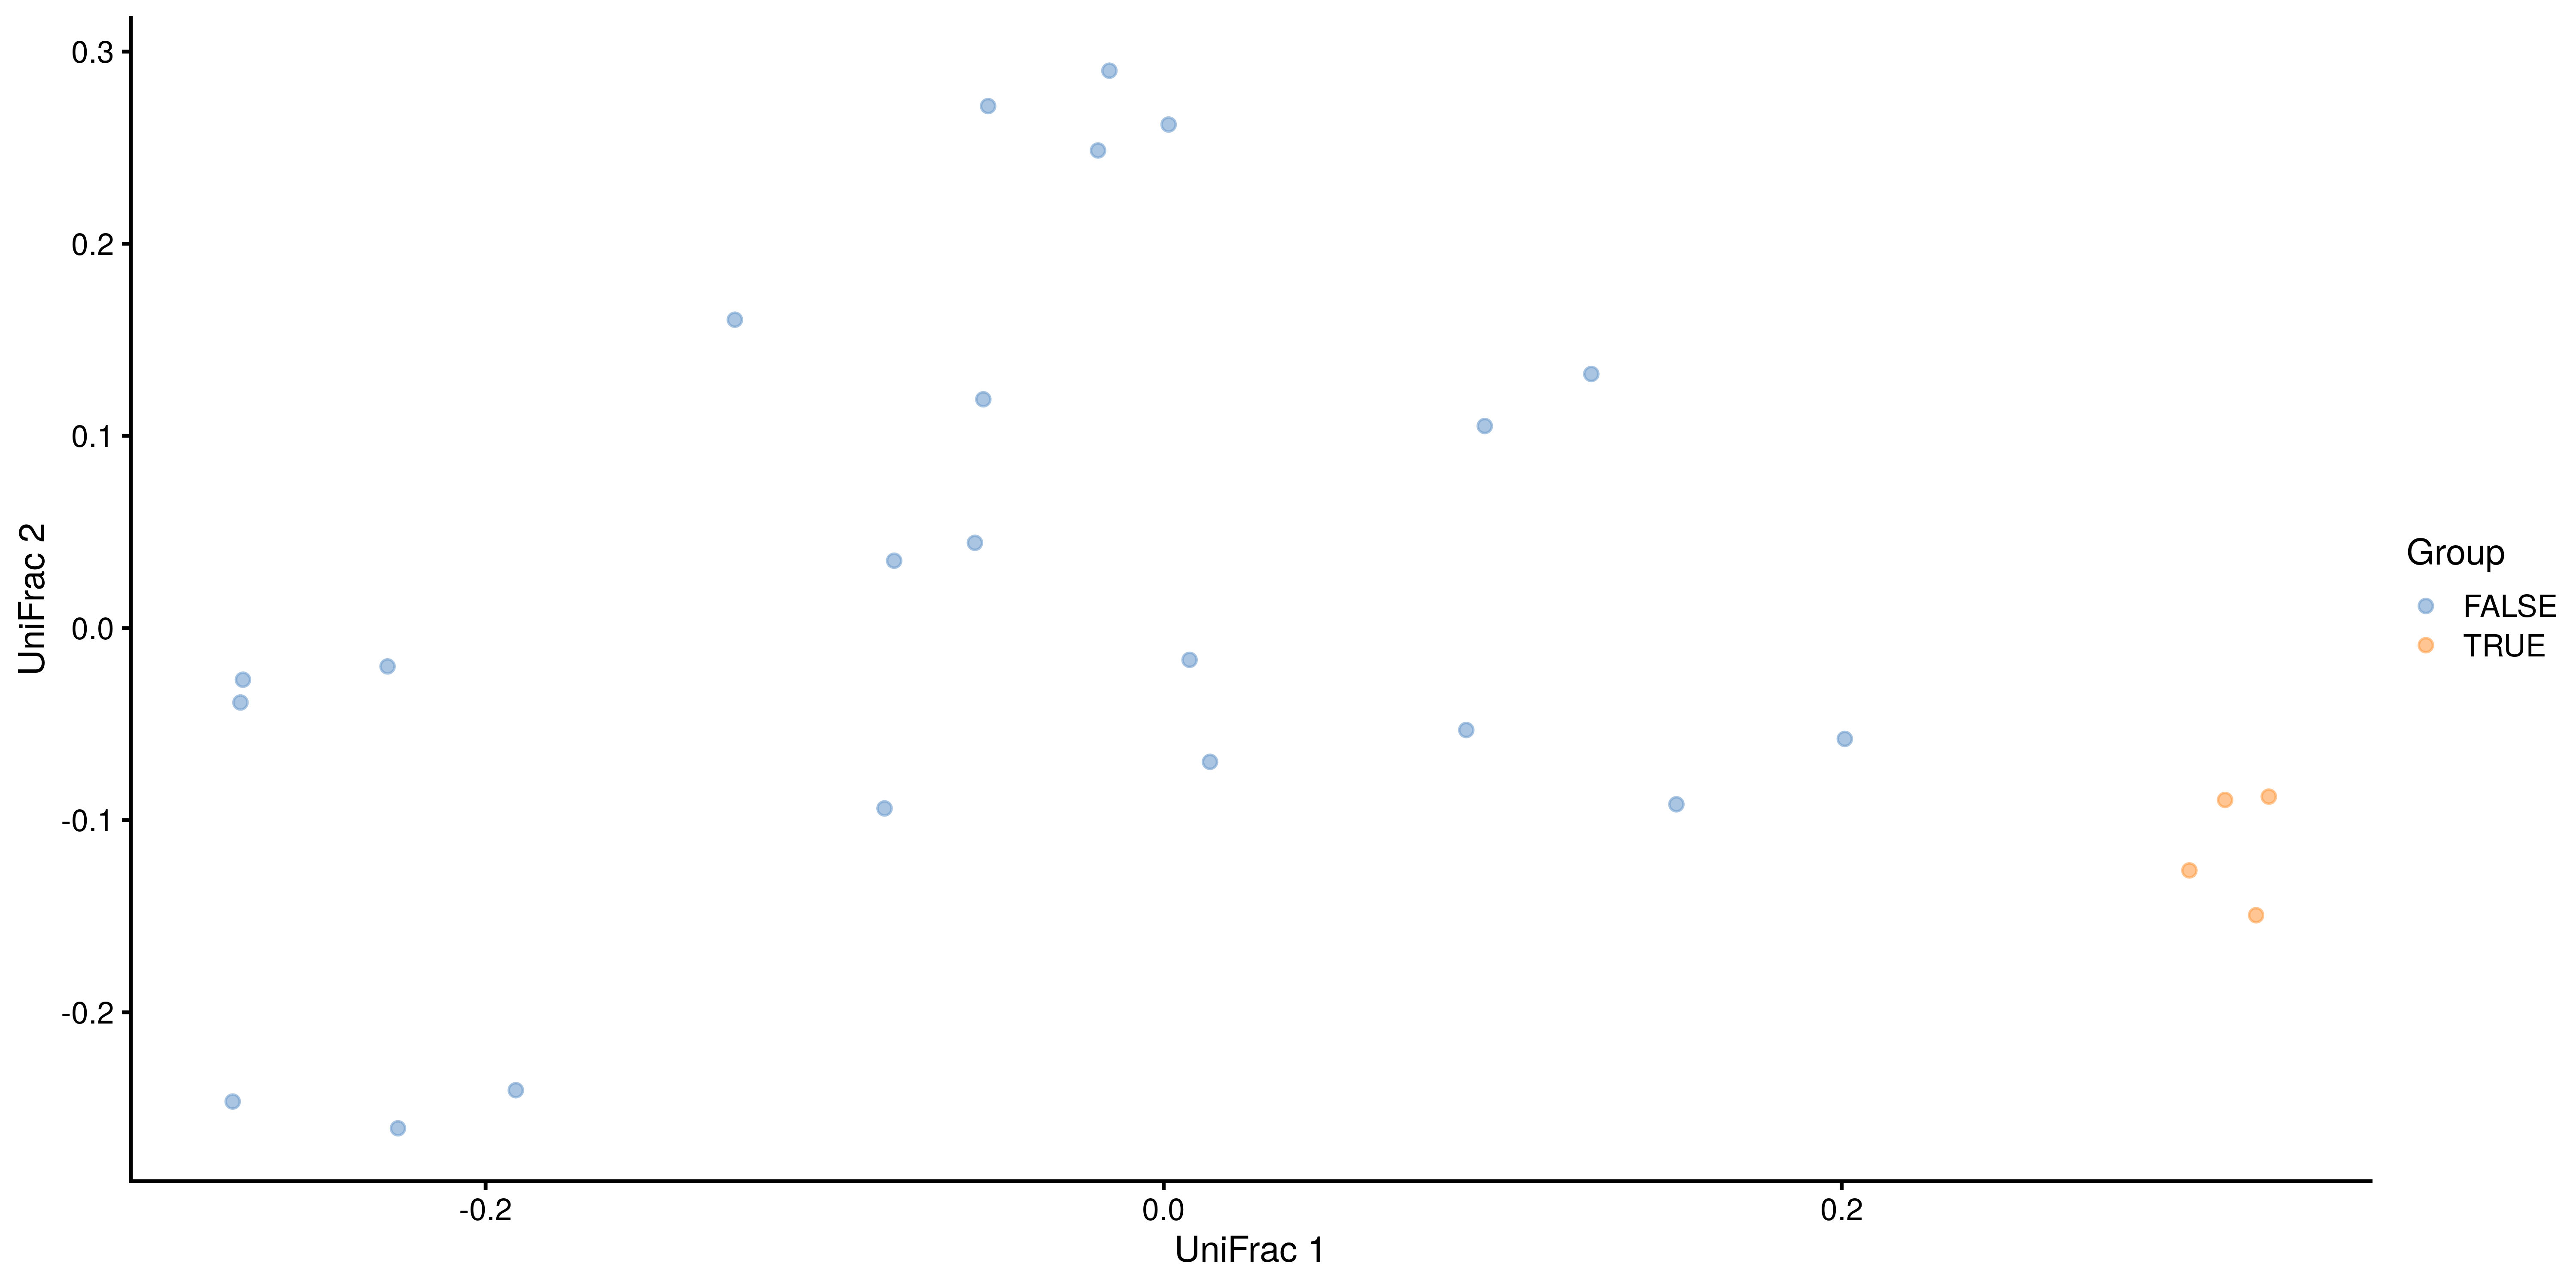
\includegraphics{20_beta_diversity_files/figure-latex/plot-unifrac-1.png}
\caption{\label{fig:plot-unifrac}Unifrac distances scaled by MDS of the GlobalPattern dataset.}
\end{figure}

\hypertarget{other-ordination-methods}{%
\section{Other ordination methods}\label{other-ordination-methods}}

Other dimension reduction methods, such as \texttt{PCA}, \texttt{t-SNE} and \texttt{UMAP} are
inherited directly from the \texttt{scater} package.

\begin{Shaded}
\begin{Highlighting}[]
\NormalTok{tse }\OtherTok{\textless{}{-}} \FunctionTok{runPCA}\NormalTok{(tse, }\AttributeTok{name =} \StringTok{"PCA"}\NormalTok{, }\AttributeTok{exprs\_values =} \StringTok{"counts"}\NormalTok{, }\AttributeTok{ncomponents =} \DecValTok{10}\NormalTok{)}
\end{Highlighting}
\end{Shaded}

\begin{Shaded}
\begin{Highlighting}[]
\FunctionTok{plotReducedDim}\NormalTok{(tse, }\StringTok{"PCA"}\NormalTok{, }\AttributeTok{colour\_by =} \StringTok{"Group"}\NormalTok{)}
\end{Highlighting}
\end{Shaded}

\begin{figure}
\centering
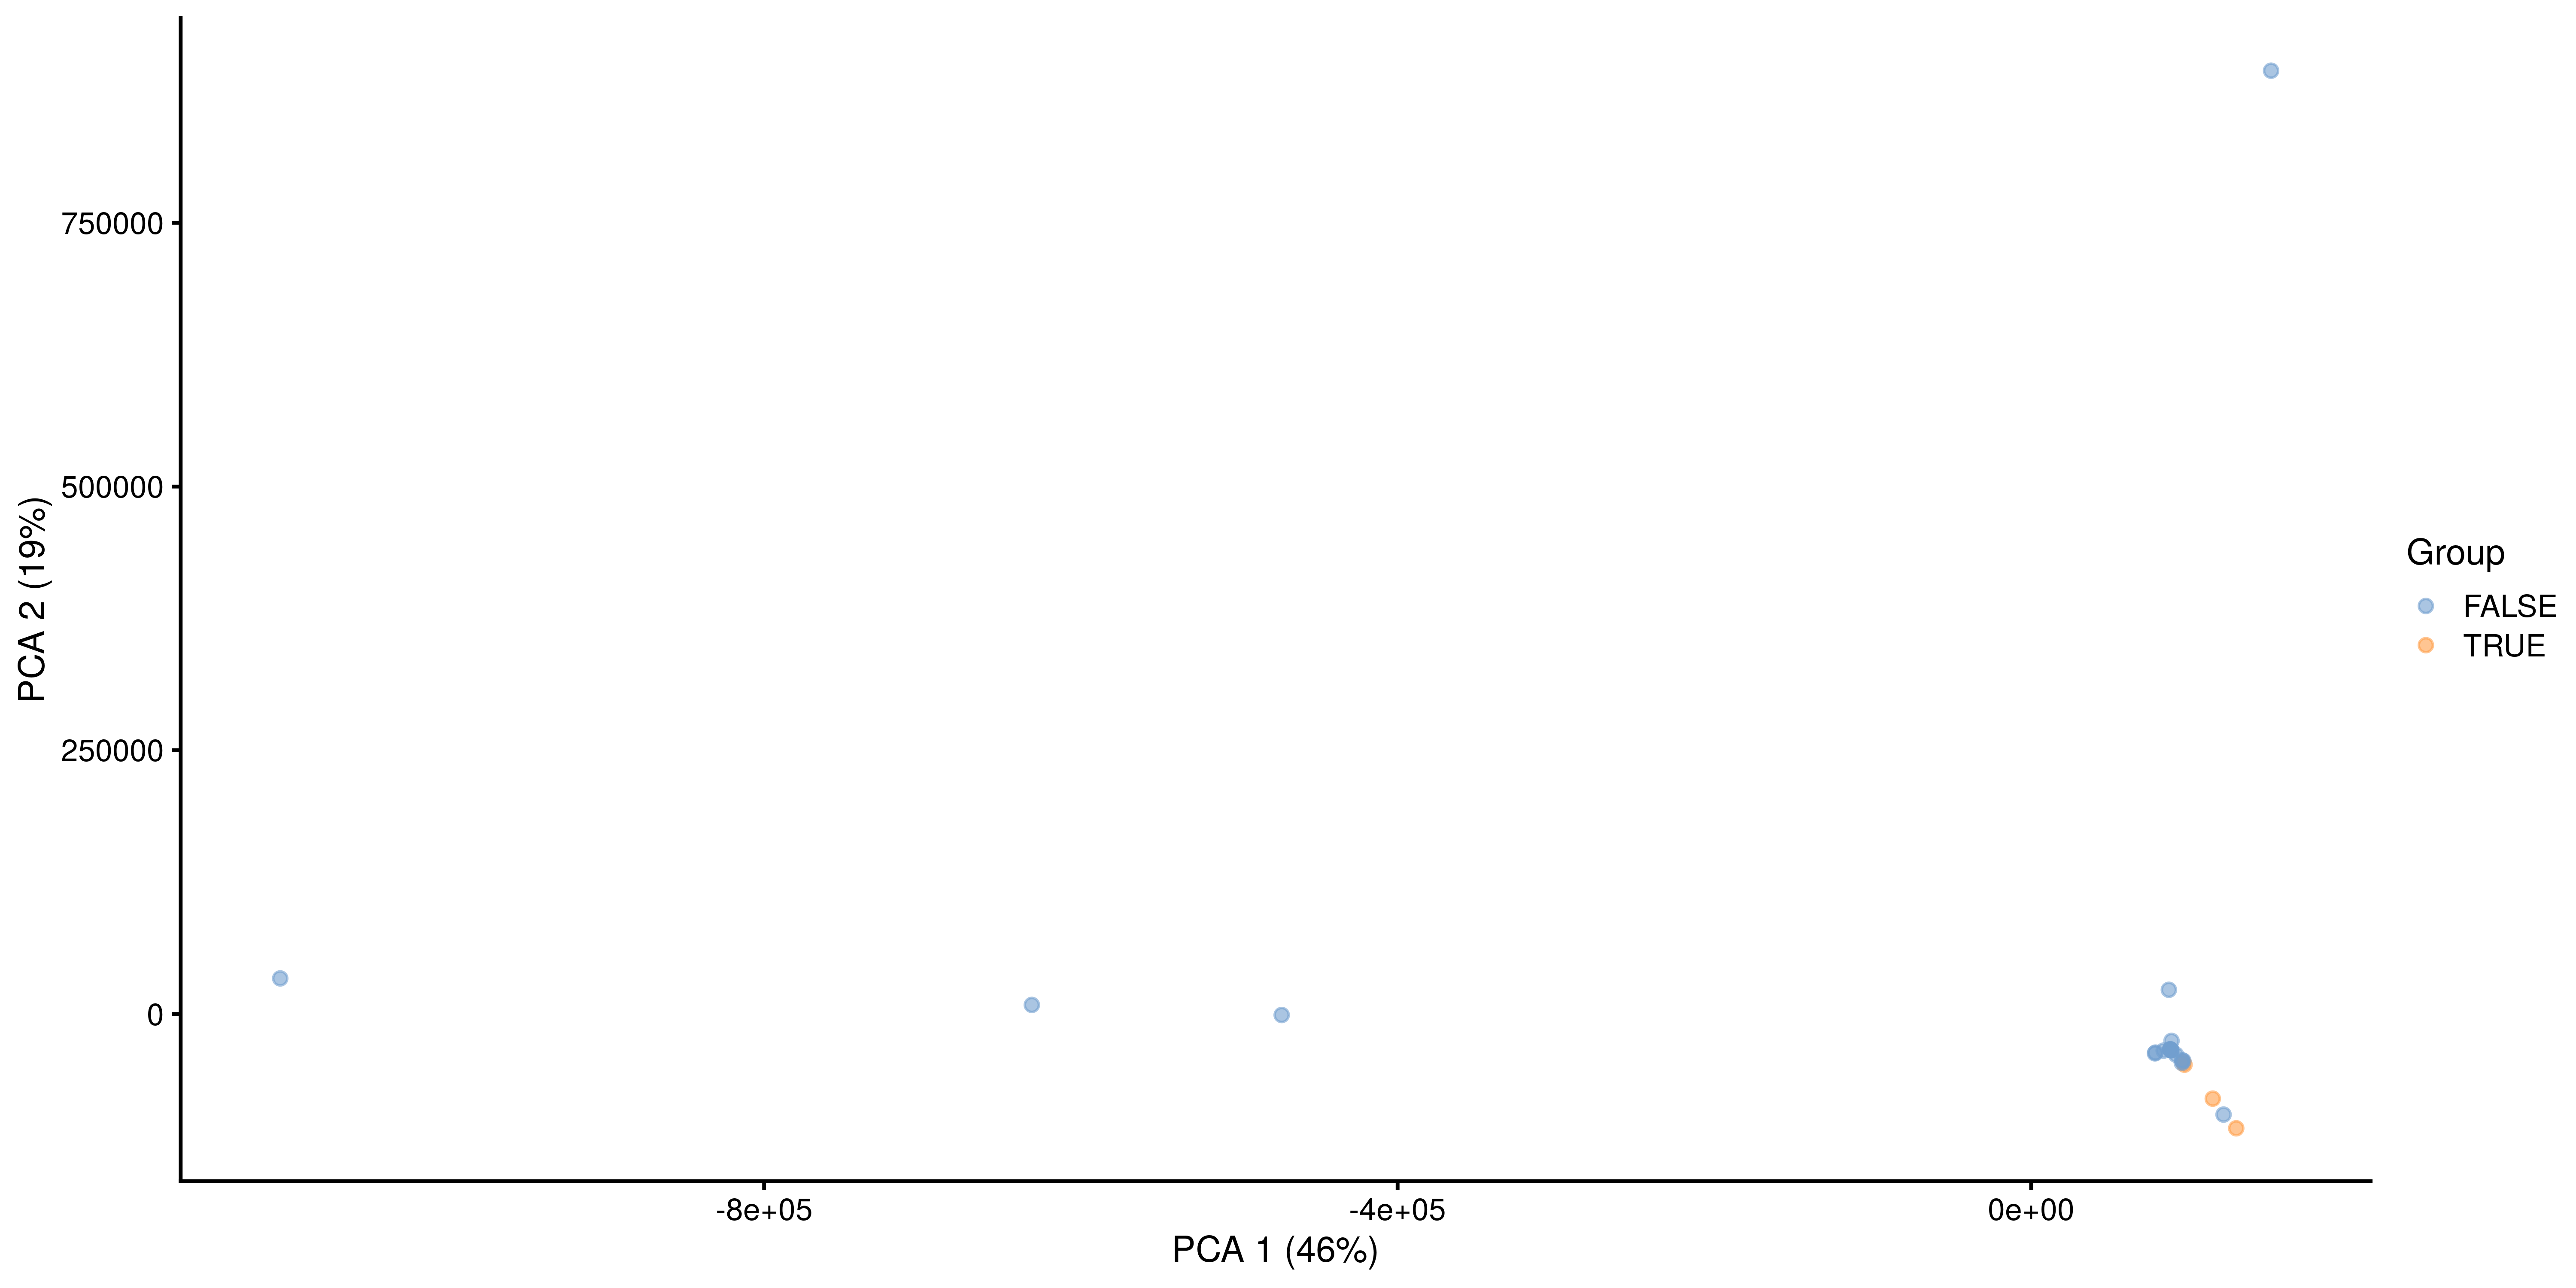
\includegraphics{20_beta_diversity_files/figure-latex/plot-pca-1.png}
\caption{\label{fig:plot-pca}PCA plot on the GlobalPatterns data set containing sample from different sources.}
\end{figure}

As mentioned before, applicability of the different methods depends on your
sample set.

FIXME: let us switch to UMAP for the examples?

\begin{Shaded}
\begin{Highlighting}[]
\NormalTok{tse }\OtherTok{\textless{}{-}} \FunctionTok{runTSNE}\NormalTok{(tse, }\AttributeTok{name =} \StringTok{"TSNE"}\NormalTok{, }\AttributeTok{exprs\_values =} \StringTok{"counts"}\NormalTok{, }\AttributeTok{ncomponents =} \DecValTok{3}\NormalTok{)}
\end{Highlighting}
\end{Shaded}

\begin{Shaded}
\begin{Highlighting}[]
\FunctionTok{plotReducedDim}\NormalTok{(tse, }\StringTok{"TSNE"}\NormalTok{, }\AttributeTok{colour\_by =} \StringTok{"Group"}\NormalTok{, }\AttributeTok{ncomponents =} \FunctionTok{c}\NormalTok{(}\DecValTok{1}\SpecialCharTok{:}\DecValTok{3}\NormalTok{))}
\end{Highlighting}
\end{Shaded}

\begin{figure}
\centering
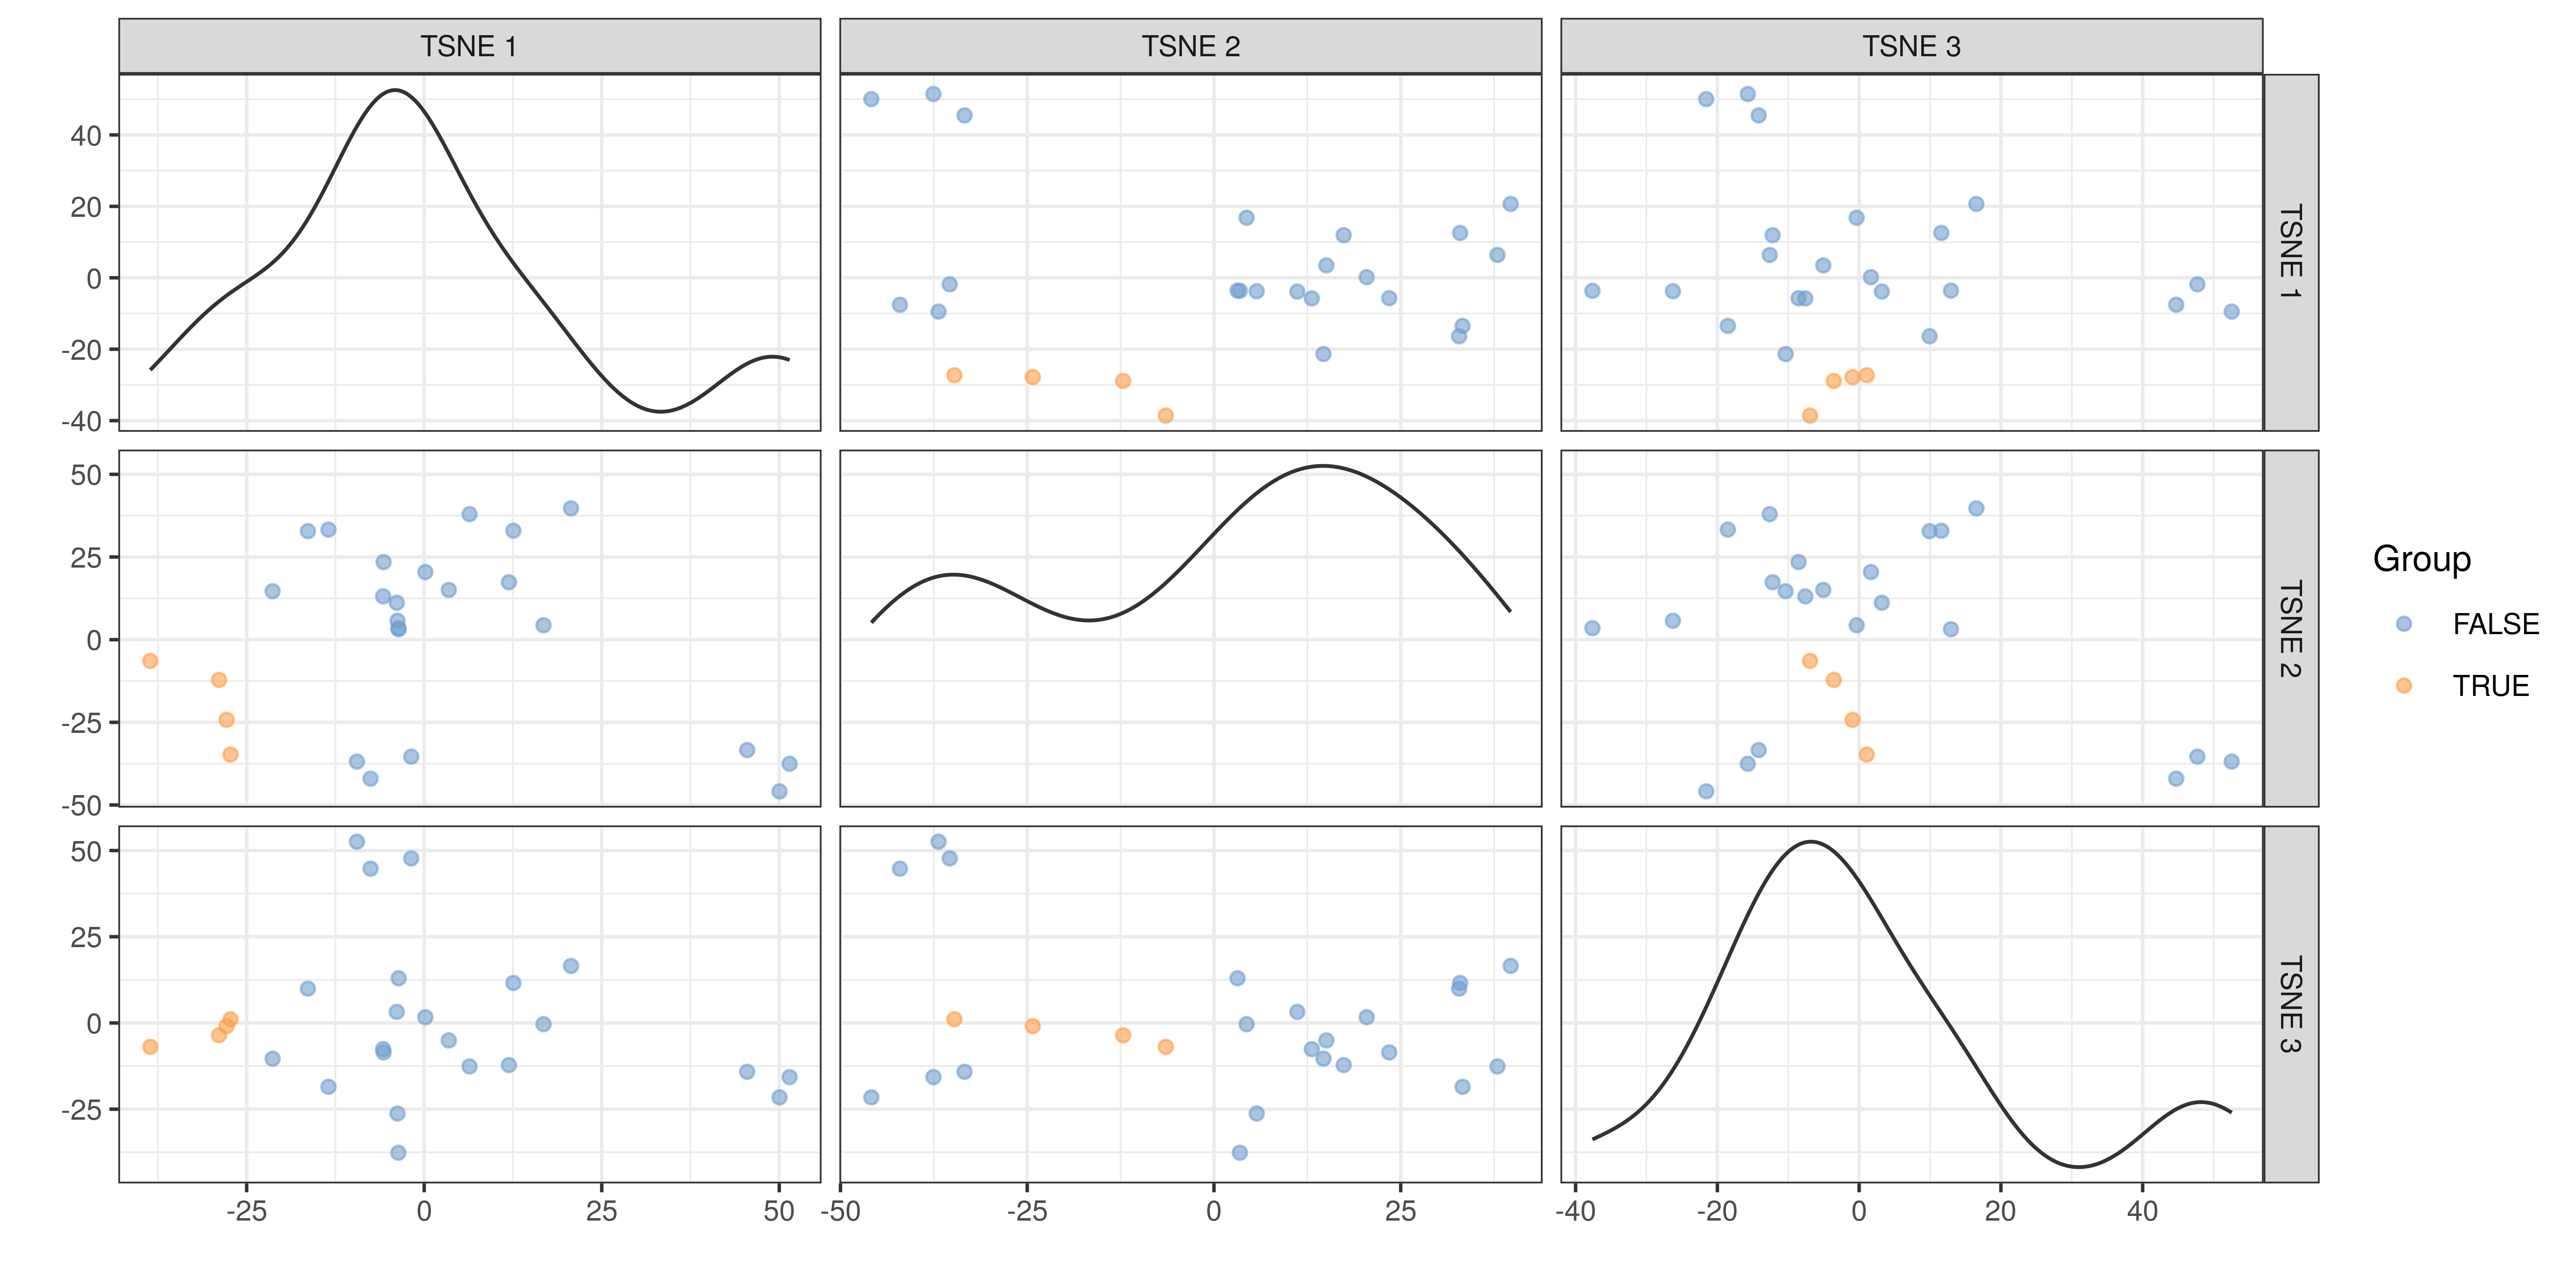
\includegraphics{20_beta_diversity_files/figure-latex/plot-tsne-1.png}
\caption{\label{fig:plot-tsne}t-SNE plot on the GlobalPatterns data set containing sample from different sources.}
\end{figure}

As a final note, \texttt{mia} provides functions for the evaluation of additional dissimilarity indices, such as:
* \texttt{calculateJSD}, \texttt{runJSD} (Jensen-Shannon divergence)
* \texttt{calculateNMDS}, \texttt{plotNMDS} (non-metric multi-dimensional scaling)
* \texttt{calculateCCA}, \texttt{runCCA} (Canonical Correspondence Analysis)
* \texttt{calculateRDA}, \texttt{runRDA} (Redundancy Analysis)
* \texttt{calculateOverlap}, \texttt{runOverlap} ()
* \texttt{calculateDPCoA}, \texttt{runDPCoA} (Double Principal Coordinate Analysis)

\hypertarget{visualizing-the-most-dominant-genus-on-pcoa}{%
\section{Visualizing the most dominant genus on PCoA}\label{visualizing-the-most-dominant-genus-on-pcoa}}

In this section we visualize most dominant genus on PCoA. A similar visualization was proposed in \href{https://www.nature.com/articles/s41467-021-22962-y}{Taxonomic signatures of cause-specific mortality risk in human gut microbiome}, Salosensaari et al.~(2021).

Let us agglomerate the data at a Genus level and getting the dominant taxa per sample.

\begin{Shaded}
\begin{Highlighting}[]
\CommentTok{\# Agglomerate to genus level}
\NormalTok{tse\_Genus }\OtherTok{\textless{}{-}} \FunctionTok{agglomerateByRank}\NormalTok{(tse, }\AttributeTok{rank=}\StringTok{"Genus"}\NormalTok{)}
\CommentTok{\# Convert to relative abundances}
\NormalTok{tse\_Genus }\OtherTok{\textless{}{-}} \FunctionTok{transformSamples}\NormalTok{(tse, }\AttributeTok{method =} \StringTok{"relabundance"}\NormalTok{, }\AttributeTok{abund\_values=}\StringTok{"counts"}\NormalTok{)}
\CommentTok{\# Add info on dominant genus per sample}
\NormalTok{tse\_Genus }\OtherTok{\textless{}{-}} \FunctionTok{addPerSampleDominantTaxa}\NormalTok{(tse\_Genus, }\AttributeTok{abund\_values=}\StringTok{"relabundance"}\NormalTok{, }\AttributeTok{name =} \StringTok{"dominant\_taxa"}\NormalTok{)}
\end{Highlighting}
\end{Shaded}

Performing PCoA with Bray-Curtis dissimilarity.

\begin{Shaded}
\begin{Highlighting}[]
\NormalTok{tse\_Genus }\OtherTok{\textless{}{-}} \FunctionTok{runMDS}\NormalTok{(tse\_Genus, }\AttributeTok{FUN =}\NormalTok{ vegan}\SpecialCharTok{::}\NormalTok{vegdist,}
              \AttributeTok{name =} \StringTok{"PCoA\_BC"}\NormalTok{, }\AttributeTok{exprs\_values =} \StringTok{"relabundance"}\NormalTok{)}
\end{Highlighting}
\end{Shaded}

Getting top taxa and visualizing the abundance on PCoA.

\begin{Shaded}
\begin{Highlighting}[]
\CommentTok{\# Getting the top taxa}
\NormalTok{top\_taxa }\OtherTok{\textless{}{-}} \FunctionTok{getTopTaxa}\NormalTok{(tse\_Genus,}\AttributeTok{top =} \DecValTok{6}\NormalTok{, }\AttributeTok{abund\_values =} \StringTok{"relabundance"}\NormalTok{)}

\CommentTok{\# Naming all the rest of non top{-}taxa as "Other"}
\NormalTok{most\_abundant }\OtherTok{\textless{}{-}} \FunctionTok{lapply}\NormalTok{(}\FunctionTok{colData}\NormalTok{(tse\_Genus)}\SpecialCharTok{$}\NormalTok{dominant\_taxa,}
                   \ControlFlowTok{function}\NormalTok{(x)\{}\ControlFlowTok{if}\NormalTok{ (x }\SpecialCharTok{\%in\%}\NormalTok{ top\_taxa) \{x\} }\ControlFlowTok{else}\NormalTok{ \{}\StringTok{"Other"}\NormalTok{\}\})}

\CommentTok{\# Storing the previous results as a new column within colData}
\FunctionTok{colData}\NormalTok{(tse\_Genus)}\SpecialCharTok{$}\NormalTok{most\_abundant }\OtherTok{\textless{}{-}} \FunctionTok{as.character}\NormalTok{(most\_abundant)}

\CommentTok{\# Calculating percentage of the most abundant}
\NormalTok{most\_abundant\_freq }\OtherTok{\textless{}{-}} \FunctionTok{table}\NormalTok{(}\FunctionTok{as.character}\NormalTok{(most\_abundant))}
\NormalTok{most\_abundant\_percent }\OtherTok{\textless{}{-}} \FunctionTok{round}\NormalTok{(most\_abundant\_freq}\SpecialCharTok{/}\FunctionTok{sum}\NormalTok{(most\_abundant\_freq)}\SpecialCharTok{*}\DecValTok{100}\NormalTok{, }\DecValTok{1}\NormalTok{)}

\CommentTok{\# Retrieving the explained variance}
\NormalTok{e }\OtherTok{\textless{}{-}} \FunctionTok{attr}\NormalTok{(}\FunctionTok{reducedDim}\NormalTok{(tse\_Genus, }\StringTok{"PCoA\_BC"}\NormalTok{), }\StringTok{"eig"}\NormalTok{);}
\NormalTok{var\_explained }\OtherTok{\textless{}{-}}\NormalTok{ e}\SpecialCharTok{/}\FunctionTok{sum}\NormalTok{(e[e}\SpecialCharTok{\textgreater{}}\DecValTok{0}\NormalTok{])}\SpecialCharTok{*}\DecValTok{100}

\CommentTok{\# Visualization}
\NormalTok{plot }\OtherTok{\textless{}{-}}\FunctionTok{plotReducedDim}\NormalTok{(tse\_Genus,}\StringTok{"PCoA\_BC"}\NormalTok{, }\AttributeTok{colour\_by =} \StringTok{"most\_abundant"}\NormalTok{) }\SpecialCharTok{+}
  \FunctionTok{scale\_colour\_manual}\NormalTok{(}\AttributeTok{values =} \FunctionTok{c}\NormalTok{(}\StringTok{"black"}\NormalTok{, }\StringTok{"blue"}\NormalTok{, }\StringTok{"lightblue"}\NormalTok{, }\StringTok{"darkgray"}\NormalTok{, }\StringTok{"magenta"}\NormalTok{, }\StringTok{"darkgreen"}\NormalTok{, }\StringTok{"red"}\NormalTok{),}
                      \AttributeTok{labels=}\FunctionTok{paste0}\NormalTok{(}\FunctionTok{names}\NormalTok{(most\_abundant\_percent),}\StringTok{"("}\NormalTok{,most\_abundant\_percent,}\StringTok{"\%)"}\NormalTok{))}\SpecialCharTok{+}
  \FunctionTok{labs}\NormalTok{(}\AttributeTok{x=}\FunctionTok{paste}\NormalTok{(}\StringTok{"PC 1 ("}\NormalTok{,}\FunctionTok{round}\NormalTok{(var\_explained[}\DecValTok{1}\NormalTok{],}\DecValTok{1}\NormalTok{),}\StringTok{"\%)"}\NormalTok{),}
       \AttributeTok{y=}\FunctionTok{paste}\NormalTok{(}\StringTok{"PC 2 ("}\NormalTok{,}\FunctionTok{round}\NormalTok{(var\_explained[}\DecValTok{2}\NormalTok{],}\DecValTok{1}\NormalTok{),}\StringTok{"\%)"}\NormalTok{),}
       \AttributeTok{color=}\StringTok{""}\NormalTok{)}
\NormalTok{plot}
\end{Highlighting}
\end{Shaded}

\includegraphics{20_beta_diversity_files/figure-latex/unnamed-chunk-7-1.png}

Note: A 3D interactive version of the earlier plot can be found from \href{https://microbiome.github.io/OMA/interactive-3d-plots.html}{here}.

Similarly let's visualize and compare the sub-population.

\begin{Shaded}
\begin{Highlighting}[]
\CommentTok{\# Calculating the frequencies and percentages for both categories}
\NormalTok{freq\_TRUE }\OtherTok{\textless{}{-}} \FunctionTok{table}\NormalTok{(}\FunctionTok{as.character}\NormalTok{(most\_abundant[}\FunctionTok{colData}\NormalTok{(tse\_Genus)}\SpecialCharTok{$}\NormalTok{Group}\SpecialCharTok{==}\ConstantTok{TRUE}\NormalTok{]))}
\NormalTok{freq\_FALSE }\OtherTok{\textless{}{-}} \FunctionTok{table}\NormalTok{(}\FunctionTok{as.character}\NormalTok{(most\_abundant[}\FunctionTok{colData}\NormalTok{(tse\_Genus)}\SpecialCharTok{$}\NormalTok{Group}\SpecialCharTok{==}\ConstantTok{FALSE}\NormalTok{]))}
\NormalTok{percent\_TRUE }\OtherTok{\textless{}{-}} \FunctionTok{round}\NormalTok{(freq\_TRUE}\SpecialCharTok{/}\FunctionTok{sum}\NormalTok{(freq\_TRUE)}\SpecialCharTok{*}\DecValTok{100}\NormalTok{, }\DecValTok{1}\NormalTok{)}
\NormalTok{percent\_FALSE }\OtherTok{\textless{}{-}} \FunctionTok{round}\NormalTok{(freq\_FALSE}\SpecialCharTok{/}\FunctionTok{sum}\NormalTok{(freq\_FALSE)}\SpecialCharTok{*}\DecValTok{100}\NormalTok{, }\DecValTok{1}\NormalTok{)}

\CommentTok{\# Visualization}
\FunctionTok{plotReducedDim}\NormalTok{(tse\_Genus[,}\FunctionTok{colData}\NormalTok{(tse\_Genus)}\SpecialCharTok{$}\NormalTok{Group}\SpecialCharTok{==}\ConstantTok{TRUE}\NormalTok{],}
                          \StringTok{"PCoA\_BC"}\NormalTok{, }\AttributeTok{colour\_by =} \StringTok{"most\_abundant"}\NormalTok{) }\SpecialCharTok{+}
  \FunctionTok{scale\_colour\_manual}\NormalTok{(}\AttributeTok{values =} \FunctionTok{c}\NormalTok{(}\StringTok{"black"}\NormalTok{, }\StringTok{"blue"}\NormalTok{, }\StringTok{"lightblue"}\NormalTok{, }\StringTok{"darkgray"}\NormalTok{, }\StringTok{"magenta"}\NormalTok{, }\StringTok{"darkgreen"}\NormalTok{, }\StringTok{"red"}\NormalTok{),}
                      \AttributeTok{labels=}\FunctionTok{paste0}\NormalTok{(}\FunctionTok{names}\NormalTok{(percent\_TRUE),}\StringTok{"("}\NormalTok{,percent\_TRUE,}\StringTok{"\%)"}\NormalTok{))}\SpecialCharTok{+}
  \FunctionTok{labs}\NormalTok{(}\AttributeTok{x=}\FunctionTok{paste}\NormalTok{(}\StringTok{"PC 1 ("}\NormalTok{,}\FunctionTok{round}\NormalTok{(var\_explained[}\DecValTok{1}\NormalTok{],}\DecValTok{1}\NormalTok{),}\StringTok{"\%)"}\NormalTok{),}
       \AttributeTok{y=}\FunctionTok{paste}\NormalTok{(}\StringTok{"PC 2 ("}\NormalTok{,}\FunctionTok{round}\NormalTok{(var\_explained[}\DecValTok{2}\NormalTok{],}\DecValTok{1}\NormalTok{),}\StringTok{"\%)"}\NormalTok{),}
       \AttributeTok{title =} \StringTok{"Group = TRUE"}\NormalTok{, }\AttributeTok{color=}\StringTok{""}\NormalTok{)}
\end{Highlighting}
\end{Shaded}

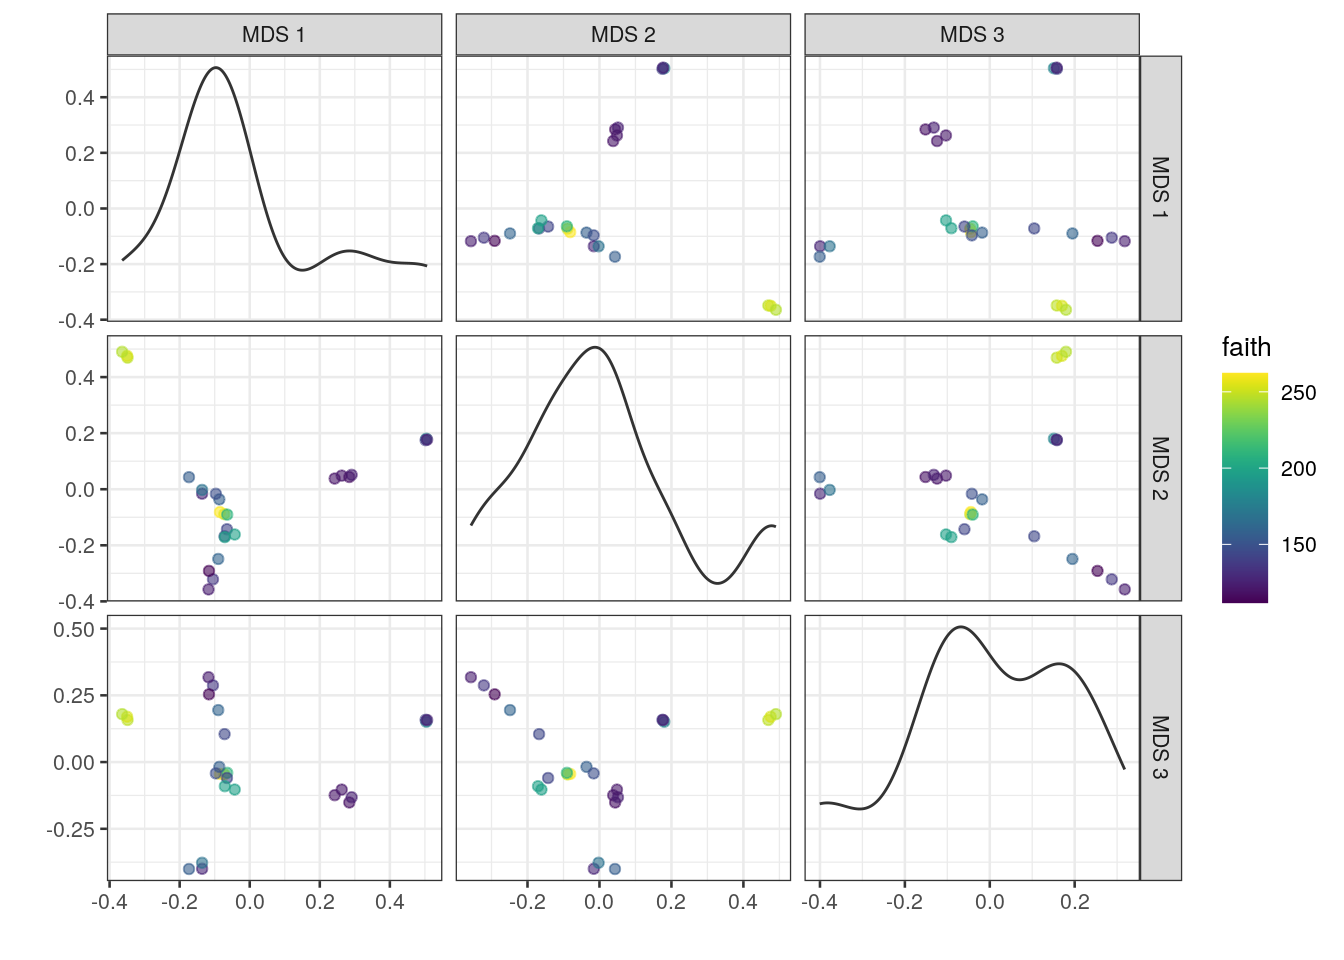
\includegraphics{20_beta_diversity_files/figure-latex/unnamed-chunk-8-1.png}

\begin{Shaded}
\begin{Highlighting}[]
\FunctionTok{plotReducedDim}\NormalTok{(tse\_Genus[,}\FunctionTok{colData}\NormalTok{(tse\_Genus)}\SpecialCharTok{$}\NormalTok{Group}\SpecialCharTok{==}\ConstantTok{FALSE}\NormalTok{],}
                          \StringTok{"PCoA\_BC"}\NormalTok{, }\AttributeTok{colour\_by =} \StringTok{"most\_abundant"}\NormalTok{) }\SpecialCharTok{+}
  \FunctionTok{scale\_colour\_manual}\NormalTok{(}\AttributeTok{values =} \FunctionTok{c}\NormalTok{(}\StringTok{"black"}\NormalTok{, }\StringTok{"blue"}\NormalTok{, }\StringTok{"lightblue"}\NormalTok{, }\StringTok{"darkgray"}\NormalTok{, }\StringTok{"magenta"}\NormalTok{, }\StringTok{"darkgreen"}\NormalTok{, }\StringTok{"red"}\NormalTok{),}
                      \AttributeTok{labels=}\FunctionTok{paste0}\NormalTok{(}\FunctionTok{names}\NormalTok{(percent\_FALSE),}\StringTok{"("}\NormalTok{,percent\_FALSE,}\StringTok{"\%)"}\NormalTok{))}\SpecialCharTok{+}
  \FunctionTok{labs}\NormalTok{(}\AttributeTok{x=}\FunctionTok{paste}\NormalTok{(}\StringTok{"PC 1 ("}\NormalTok{,}\FunctionTok{round}\NormalTok{(var\_explained[}\DecValTok{1}\NormalTok{],}\DecValTok{1}\NormalTok{),}\StringTok{"\%)"}\NormalTok{),}
       \AttributeTok{y=}\FunctionTok{paste}\NormalTok{(}\StringTok{"PC 2 ("}\NormalTok{,}\FunctionTok{round}\NormalTok{(var\_explained[}\DecValTok{2}\NormalTok{],}\DecValTok{1}\NormalTok{),}\StringTok{"\%)"}\NormalTok{),}
       \AttributeTok{title =} \StringTok{"Group = FALSE"}\NormalTok{, }\AttributeTok{color=}\StringTok{""}\NormalTok{)}
\end{Highlighting}
\end{Shaded}

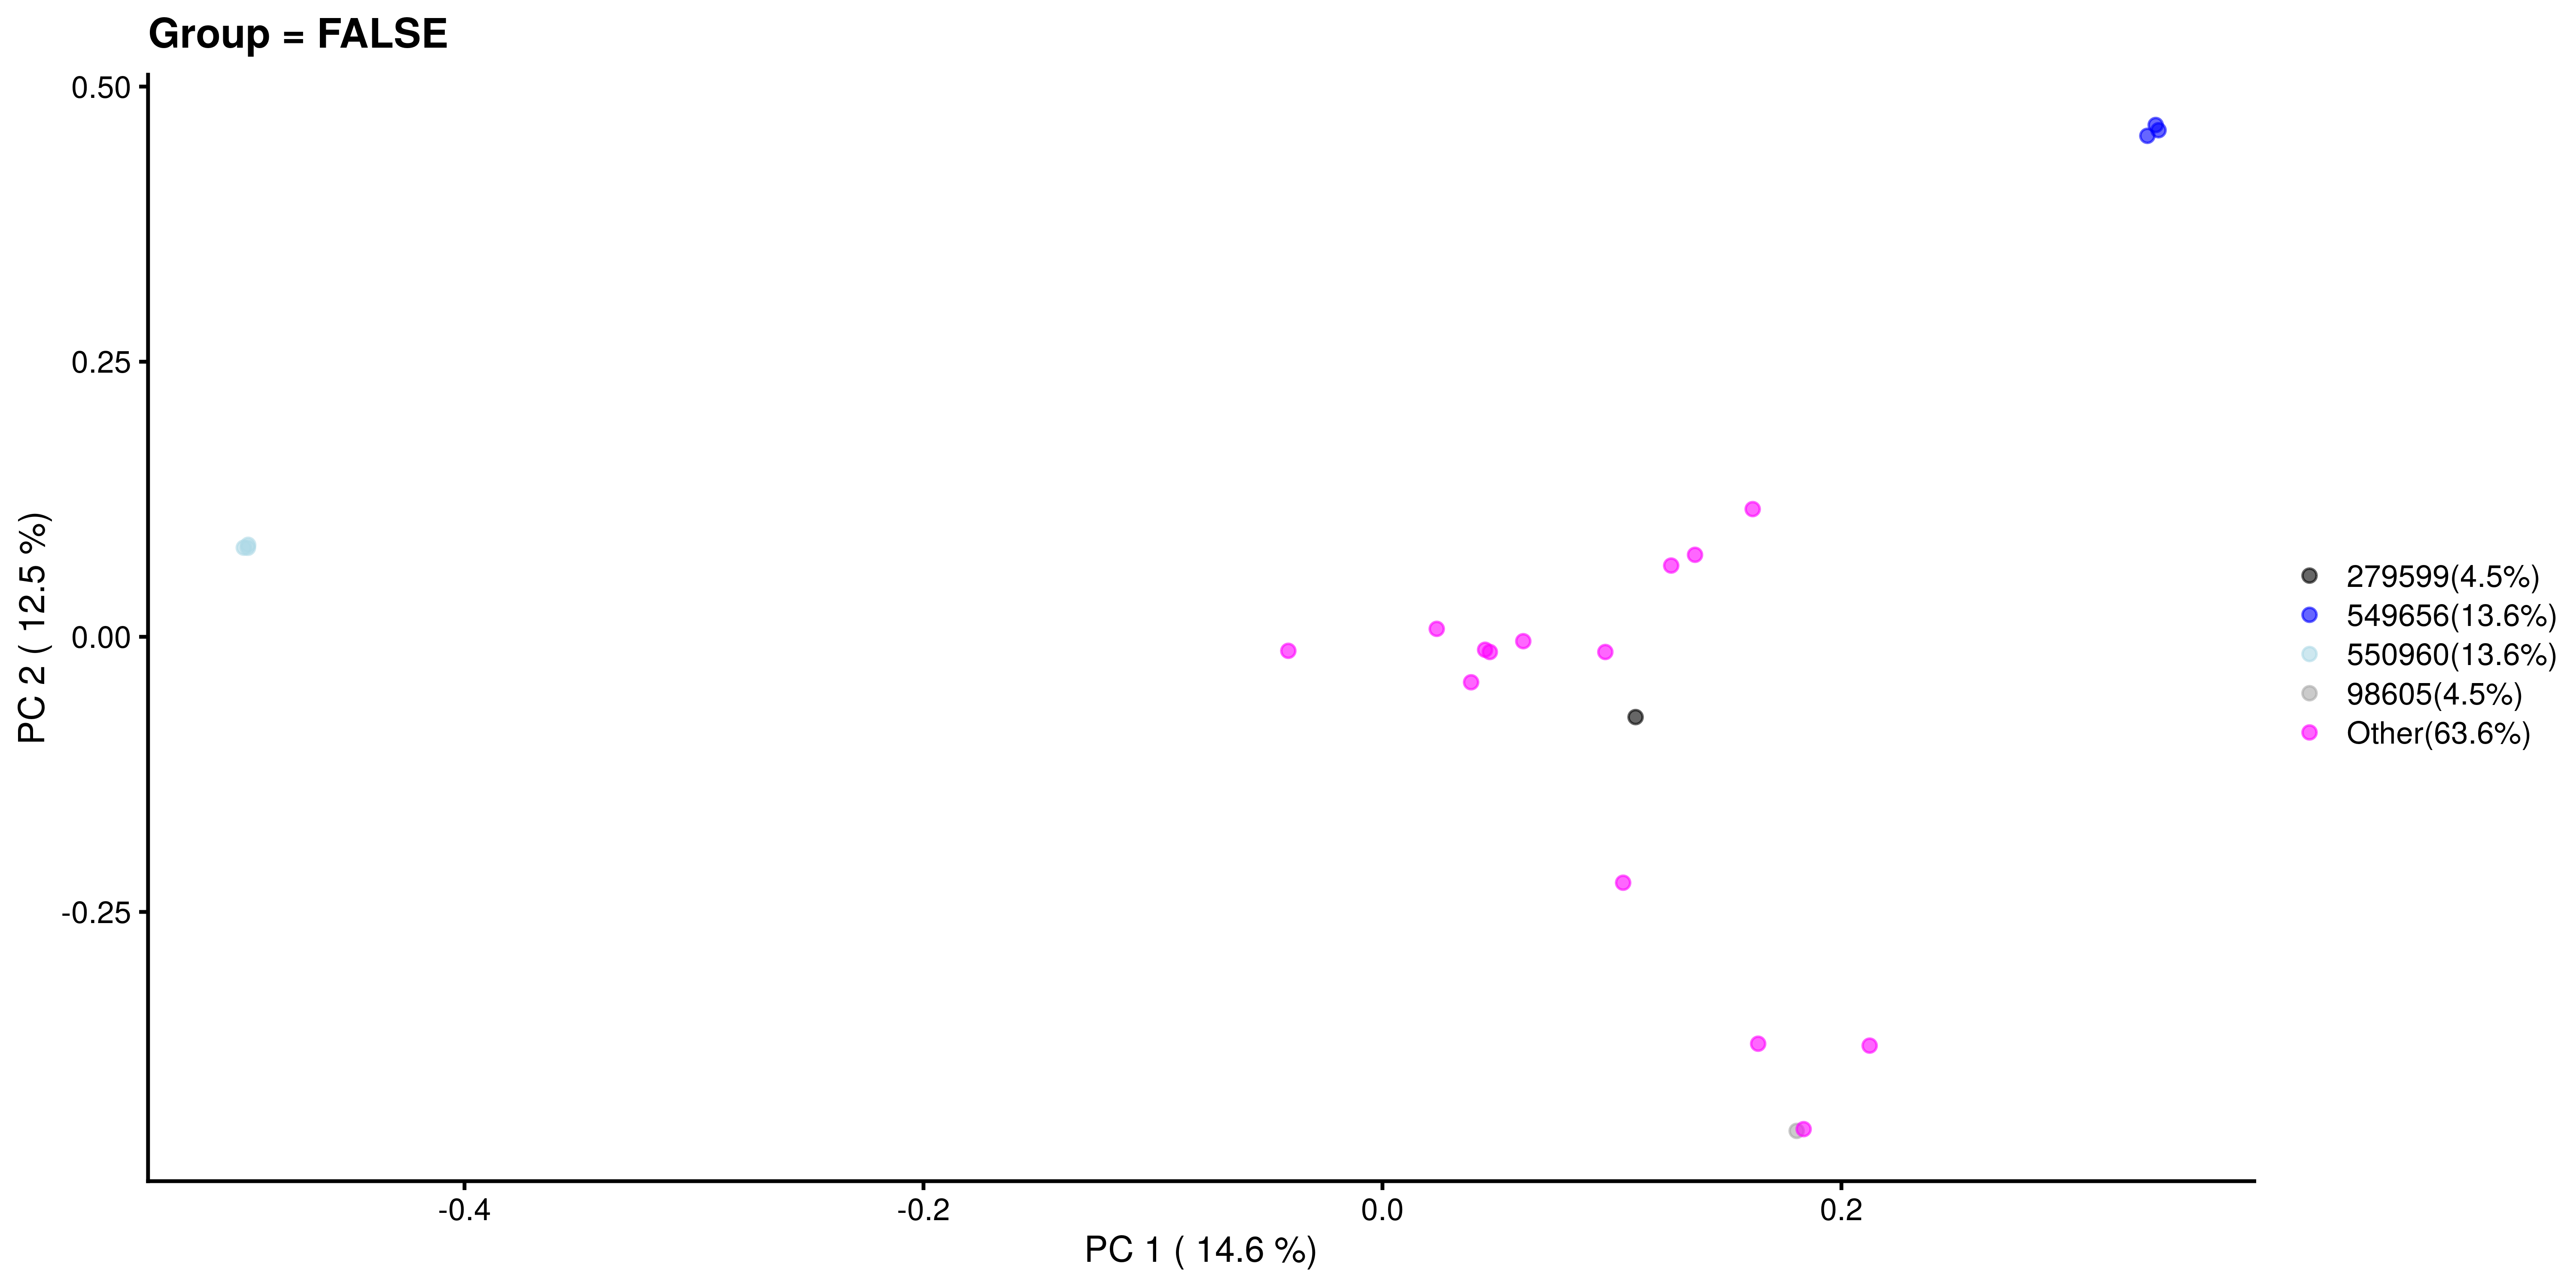
\includegraphics{20_beta_diversity_files/figure-latex/unnamed-chunk-8-2.png}

\hypertarget{testing-differences-in-community-composition-between-sample-groups}{%
\subsection{Testing differences in community composition between sample groups}\label{testing-differences-in-community-composition-between-sample-groups}}

The permutational analysis of variance (PERMANOVA) \citep{Anderson2001} is
a widely used non-parametric multivariate method that can be used to
estimate the actual statistical significance of differences in the
observed community composition between two groups of
samples.

PERMANOVA evaluates the hypothesis that the centroids and dispersion
of the community are equivalent between the compared groups. A small
p-value indicates that the compared groups have, on average, a
different community composition.

This method is implemented in the \texttt{vegan} package in the function
\href{https://www.rdocumentation.org/packages/vegan/versions/2.4-2/topics/adonis}{\texttt{adonis2}}.

We can get equal result by first performing distance-based redundancy analysis (dbRDA),
and then applying permutational test for result of redundancy analysis. Advantage is
that by doing so we can get coefficients: how much each taxa affect to the result.

\begin{Shaded}
\begin{Highlighting}[]
\ControlFlowTok{if}\NormalTok{( }\SpecialCharTok{!}\FunctionTok{require}\NormalTok{(vegan) )\{}
\NormalTok{    BiocManager}\SpecialCharTok{::}\FunctionTok{install}\NormalTok{(}\StringTok{"vegan"}\NormalTok{)}
    \FunctionTok{library}\NormalTok{(}\StringTok{"vegan"}\NormalTok{)}
\NormalTok{\}}
\CommentTok{\# Agglomerate data to Species level}
\NormalTok{tse }\OtherTok{\textless{}{-}} \FunctionTok{agglomerateByRank}\NormalTok{(tse, }\AttributeTok{rank =} \StringTok{"Species"}\NormalTok{)}

\CommentTok{\# Set seed for reproducibility}
\FunctionTok{set.seed}\NormalTok{(}\DecValTok{1576}\NormalTok{)}
\CommentTok{\# We choose 99 random permutations. Consider applying more (999 or 9999) in your}
\CommentTok{\# analysis. }
\NormalTok{permanova }\OtherTok{\textless{}{-}} \FunctionTok{adonis2}\NormalTok{(}\FunctionTok{t}\NormalTok{(}\FunctionTok{assay}\NormalTok{(tse,}\StringTok{"relabundance"}\NormalTok{)) }\SpecialCharTok{\textasciitilde{}}\NormalTok{ Group,}
                     \AttributeTok{data =} \FunctionTok{colData}\NormalTok{(tse),}
                     \AttributeTok{method =} \StringTok{"euclidean"}\NormalTok{,}
                     \AttributeTok{by =} \ConstantTok{NULL}\NormalTok{,}
                     \AttributeTok{permutations =} \DecValTok{99}\NormalTok{)}

\CommentTok{\# Set seed for reproducibility}
\FunctionTok{set.seed}\NormalTok{(}\DecValTok{1576}\NormalTok{)}
\CommentTok{\# Perform dbRDA}
\NormalTok{dbrda }\OtherTok{\textless{}{-}} \FunctionTok{dbrda}\NormalTok{(}\FunctionTok{t}\NormalTok{(}\FunctionTok{assay}\NormalTok{(tse,}\StringTok{"relabundance"}\NormalTok{)) }\SpecialCharTok{\textasciitilde{}}\NormalTok{ Group, }
               \AttributeTok{data =} \FunctionTok{colData}\NormalTok{(tse))}
\CommentTok{\# Perform permutational analysis}
\NormalTok{permanova2 }\OtherTok{\textless{}{-}} \FunctionTok{anova.cca}\NormalTok{(dbrda,}
                        \AttributeTok{method =} \StringTok{"euclidean"}\NormalTok{,}
                        \AttributeTok{permutations =} \DecValTok{99}\NormalTok{)}

\CommentTok{\# Get p{-}values}
\NormalTok{p\_values }\OtherTok{\textless{}{-}} \FunctionTok{c}\NormalTok{( permanova[}\StringTok{"Model"}\NormalTok{, }\StringTok{"Pr(\textgreater{}F)"}\NormalTok{], permanova2[}\StringTok{"Model"}\NormalTok{, }\StringTok{"Pr(\textgreater{}F)"}\NormalTok{] )}
\NormalTok{p\_values }\OtherTok{\textless{}{-}}\FunctionTok{as.data.frame}\NormalTok{(p\_values)}
\FunctionTok{rownames}\NormalTok{(p\_values) }\OtherTok{\textless{}{-}} \FunctionTok{c}\NormalTok{(}\StringTok{"adonis2"}\NormalTok{, }\StringTok{"dbRDA+anova.cca"}\NormalTok{)}
\NormalTok{p\_values}
\end{Highlighting}
\end{Shaded}

\begin{verbatim}
##                 p_values
## adonis2             0.02
## dbRDA+anova.cca     0.02
\end{verbatim}

In this case, the community composition is not significantly different
between the groups.

Let us visualize the model coefficients for species that exhibit the
largest differences between the groups. This gives some insights into
how the groups tend to differ from each other in terms of community
composition.

\begin{Shaded}
\begin{Highlighting}[]
\CommentTok{\# Add taxa info}
\FunctionTok{sppscores}\NormalTok{(dbrda) }\OtherTok{\textless{}{-}} \FunctionTok{t}\NormalTok{(}\FunctionTok{assay}\NormalTok{(tse,}\StringTok{"relabundance"}\NormalTok{))}
\CommentTok{\# Get coefficients}
\NormalTok{coef }\OtherTok{\textless{}{-}}\NormalTok{ dbrda}\SpecialCharTok{$}\NormalTok{CCA}\SpecialCharTok{$}\NormalTok{v}
\CommentTok{\# Get the taxa with biggest weights}
\NormalTok{top.coef }\OtherTok{\textless{}{-}} \FunctionTok{head}\NormalTok{( coef[}\FunctionTok{rev}\NormalTok{(}\FunctionTok{order}\NormalTok{(}\FunctionTok{abs}\NormalTok{(coef))), , }\AttributeTok{drop =} \ConstantTok{FALSE}\NormalTok{], }\DecValTok{20}\NormalTok{)}
\CommentTok{\# Sort weights in increasing order}
\NormalTok{top.coef }\OtherTok{\textless{}{-}}\NormalTok{ top.coef[ }\FunctionTok{order}\NormalTok{(top.coef), ]}
\CommentTok{\# Get top names}
\NormalTok{top\_names }\OtherTok{\textless{}{-}} \FunctionTok{names}\NormalTok{(top.coef)[ }\FunctionTok{order}\NormalTok{(}\FunctionTok{abs}\NormalTok{(top.coef), }\AttributeTok{decreasing =} \ConstantTok{TRUE}\NormalTok{) ]}
\end{Highlighting}
\end{Shaded}

\begin{Shaded}
\begin{Highlighting}[]
\FunctionTok{ggplot}\NormalTok{(}\FunctionTok{data.frame}\NormalTok{(}\AttributeTok{x =}\NormalTok{ top.coef,}
                  \AttributeTok{y =} \FunctionTok{factor}\NormalTok{(}\FunctionTok{names}\NormalTok{(top.coef),}
                                      \FunctionTok{unique}\NormalTok{(}\FunctionTok{names}\NormalTok{(top.coef)))),}
        \FunctionTok{aes}\NormalTok{(}\AttributeTok{x =}\NormalTok{ x, }\AttributeTok{y =}\NormalTok{ y)) }\SpecialCharTok{+}
    \FunctionTok{geom\_bar}\NormalTok{(}\AttributeTok{stat=}\StringTok{"identity"}\NormalTok{) }\SpecialCharTok{+}
    \FunctionTok{labs}\NormalTok{(}\AttributeTok{x=}\StringTok{""}\NormalTok{,}\AttributeTok{y=}\StringTok{""}\NormalTok{,}\AttributeTok{title=}\StringTok{"Top Taxa"}\NormalTok{) }\SpecialCharTok{+}
    \FunctionTok{theme\_bw}\NormalTok{()}
\end{Highlighting}
\end{Shaded}

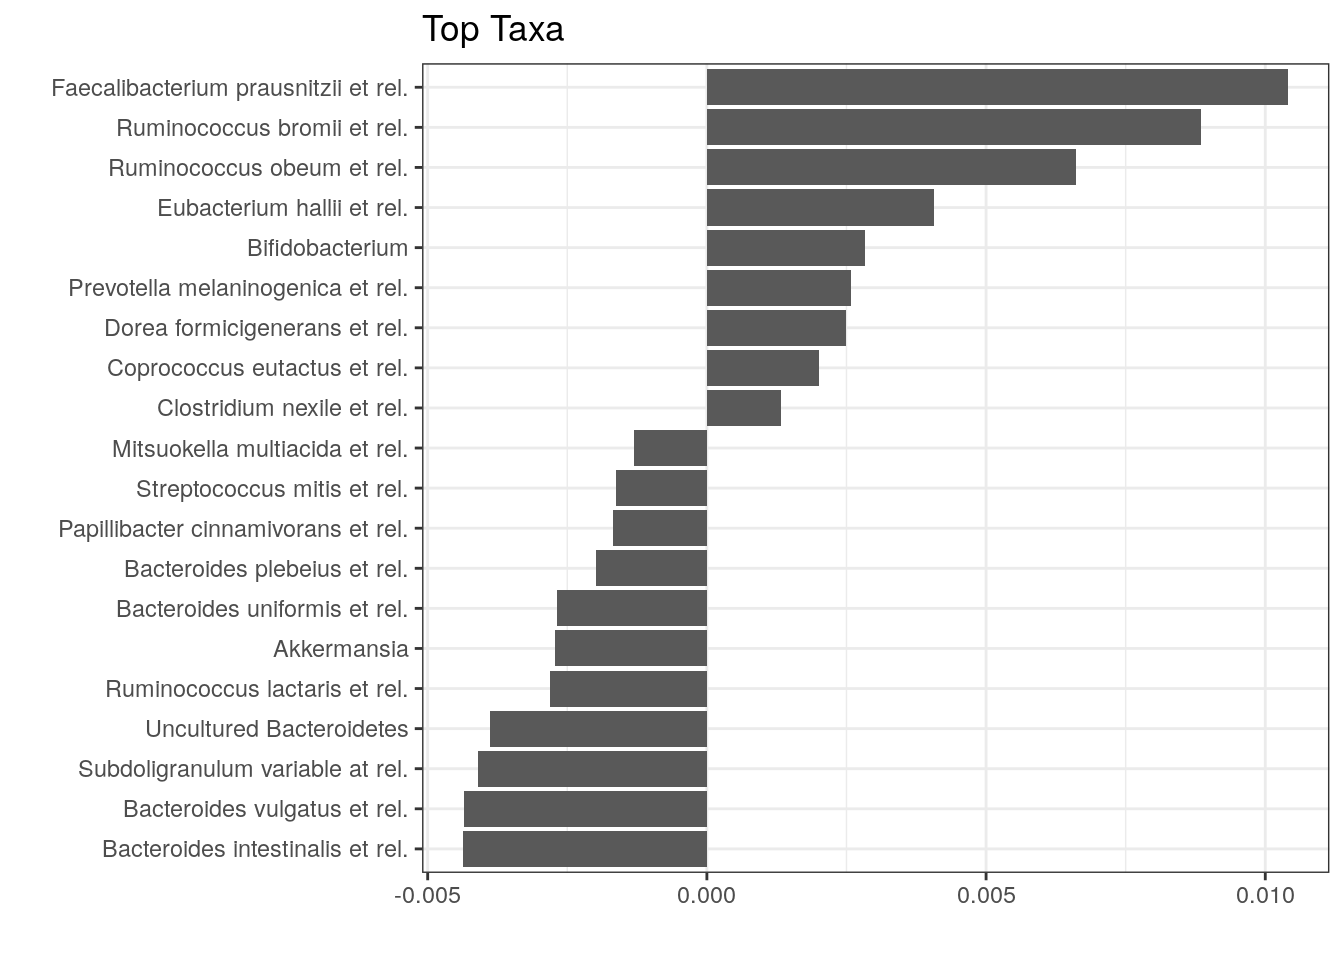
\includegraphics{20_beta_diversity_files/figure-latex/plot-top-coef-anova-1.png}

In the above example, the largest differences between the two groups
can be attributed to \emph{Genus:Bacteroides} (elevated in the first
group) and \emph{Family:Ruminococcaceae} (elevated in the second
group), and many other co-varying species.

\hypertarget{checking-the-homogeneity-condition}{%
\subsection{Checking the homogeneity condition}\label{checking-the-homogeneity-condition}}

It is important to note that the application of PERMANOVA assumes
homogeneous group dispersions (variances). This can be tested with the
PERMDISP2 method \citep{Anderson2006} by using the same assay and distance
method than in PERMANOVA.

\begin{Shaded}
\begin{Highlighting}[]
\FunctionTok{anova}\NormalTok{( }\FunctionTok{betadisper}\NormalTok{(}\FunctionTok{vegdist}\NormalTok{(}\FunctionTok{t}\NormalTok{(}\FunctionTok{assay}\NormalTok{(tse, }\StringTok{"counts"}\NormalTok{))), }\FunctionTok{colData}\NormalTok{(tse)}\SpecialCharTok{$}\NormalTok{Group) )}
\end{Highlighting}
\end{Shaded}

\begin{verbatim}
## Analysis of Variance Table
## 
## Response: Distances
##           Df Sum Sq Mean Sq F value  Pr(>F)    
## Groups     1 0.2385  0.2385     103 3.6e-10 ***
## Residuals 24 0.0554  0.0023                    
## ---
## Signif. codes:  0 '***' 0.001 '**' 0.01 '*' 0.05 '.' 0.1 ' ' 1
\end{verbatim}

If the groups have similar dispersion, PERMANOVA can be seen as an
appropriate choice for comparing community compositions.

\hypertarget{further-reading}{%
\section{Further reading}\label{further-reading}}

\begin{itemize}
\item
  \href{http://bioconductor.org/books/release/OSCA/clustering.html}{How to extract information from clusters}
\item
  Chapter \ref{community-typing} on community typing
\end{itemize}

\hypertarget{session-info-5}{%
\section*{Session Info}\label{session-info-5}}
\addcontentsline{toc}{section}{Session Info}

View session info

\begin{verbatim}
R version 4.1.2 (2021-11-01)
Platform: x86_64-pc-linux-gnu (64-bit)
Running under: Ubuntu 20.04.3 LTS

Matrix products: default
BLAS/LAPACK: /usr/lib/x86_64-linux-gnu/openblas-pthread/libopenblasp-r0.3.8.so

locale:
 [1] LC_CTYPE=en_US.UTF-8       LC_NUMERIC=C              
 [3] LC_TIME=en_US.UTF-8        LC_COLLATE=en_US.UTF-8    
 [5] LC_MONETARY=en_US.UTF-8    LC_MESSAGES=en_US.UTF-8   
 [7] LC_PAPER=en_US.UTF-8       LC_NAME=C                 
 [9] LC_ADDRESS=C               LC_TELEPHONE=C            
[11] LC_MEASUREMENT=en_US.UTF-8 LC_IDENTIFICATION=C       

attached base packages:
[1] stats4    stats     graphics  grDevices utils     datasets  methods  
[8] base     

other attached packages:
 [1] patchwork_1.1.1                scater_1.22.0                 
 [3] scuttle_1.4.0                  ggplot2_3.3.5                 
 [5] vegan_2.5-7                    lattice_0.20-45               
 [7] permute_0.9-7                  mia_1.3.19                    
 [9] MultiAssayExperiment_1.20.0    TreeSummarizedExperiment_2.1.4
[11] Biostrings_2.62.0              XVector_0.34.0                
[13] SingleCellExperiment_1.16.0    SummarizedExperiment_1.24.0   
[15] Biobase_2.54.0                 GenomicRanges_1.46.1          
[17] GenomeInfoDb_1.30.1            IRanges_2.28.0                
[19] S4Vectors_0.32.3               BiocGenerics_0.40.0           
[21] MatrixGenerics_1.6.0           matrixStats_0.61.0-9001       
[23] BiocStyle_2.22.0               rebook_1.4.0                  

loaded via a namespace (and not attached):
 [1] Rtsne_0.15                  ggbeeswarm_0.6.0           
 [3] colorspace_2.0-3            ellipsis_0.3.2             
 [5] BiocNeighbors_1.12.0        farver_2.1.0               
 [7] ggrepel_0.9.1               bit64_4.0.5                
 [9] fansi_1.0.2                 decontam_1.14.0            
[11] splines_4.1.2               codetools_0.2-18           
[13] sparseMatrixStats_1.6.0     cachem_1.0.6               
[15] knitr_1.37                  jsonlite_1.8.0             
[17] cluster_2.1.2               graph_1.72.0               
[19] BiocManager_1.30.16         compiler_4.1.2             
[21] assertthat_0.2.1            Matrix_1.4-0               
[23] fastmap_1.1.0               lazyeval_0.2.2             
[25] cli_3.2.0                   BiocSingular_1.10.0        
[27] htmltools_0.5.2             tools_4.1.2                
[29] rsvd_1.0.5                  gtable_0.3.0               
[31] glue_1.6.2                  GenomeInfoDbData_1.2.7     
[33] reshape2_1.4.4              dplyr_1.0.8                
[35] Rcpp_1.0.8.3                vctrs_0.3.8                
[37] ape_5.6-2                   nlme_3.1-155               
[39] DECIPHER_2.22.0             DelayedMatrixStats_1.16.0  
[41] xfun_0.30                   stringr_1.4.0              
[43] beachmat_2.10.0             lifecycle_1.0.1            
[45] irlba_2.3.5                 XML_3.99-0.9               
[47] zlibbioc_1.40.0             MASS_7.3-55                
[49] scales_1.1.1                parallel_4.1.2             
[51] yaml_2.3.5                  memoise_2.0.1              
[53] gridExtra_2.3               yulab.utils_0.0.4          
[55] stringi_1.7.6               RSQLite_2.2.10             
[57] highr_0.9                   ScaledMatrix_1.2.0         
[59] tidytree_0.3.9              filelock_1.0.2             
[61] BiocParallel_1.28.3         rlang_1.0.2                
[63] pkgconfig_2.0.3             bitops_1.0-7               
[65] evaluate_0.15               purrr_0.3.4                
[67] labeling_0.4.2              treeio_1.18.1              
[69] CodeDepends_0.6.5           cowplot_1.1.1              
[71] bit_4.0.4                   tidyselect_1.1.2           
[73] plyr_1.8.6                  magrittr_2.0.2             
[75] bookdown_0.25               R6_2.5.1                   
[77] generics_0.1.2              DelayedArray_0.20.0        
[79] DBI_1.1.2                   withr_2.5.0                
[81] mgcv_1.8-39                 pillar_1.7.0               
[83] RCurl_1.98-1.6              tibble_3.1.6               
[85] dir.expiry_1.2.0            crayon_1.5.0               
[87] utf8_1.2.2                  rmarkdown_2.13             
[89] viridis_0.6.2               grid_4.1.2                 
[91] blob_1.2.2                  digest_0.6.29              
[93] tidyr_1.2.0                 munsell_0.5.0              
[95] DirichletMultinomial_1.36.0 beeswarm_0.4.0             
[97] viridisLite_0.4.0           vipor_0.4.5                
\end{verbatim}

\hypertarget{microbiome-community}{%
\chapter{Community composition}\label{microbiome-community}}

\begin{verbatim}
## Loading required package: ecodist
\end{verbatim}

\begin{Shaded}
\begin{Highlighting}[]
\FunctionTok{library}\NormalTok{(mia)}
\FunctionTok{data}\NormalTok{(}\StringTok{"GlobalPatterns"}\NormalTok{, }\AttributeTok{package=}\StringTok{"mia"}\NormalTok{)}
\NormalTok{tse }\OtherTok{\textless{}{-}}\NormalTok{ GlobalPatterns}
\end{Highlighting}
\end{Shaded}

\hypertarget{visualizing-taxonomic-composition}{%
\section{Visualizing taxonomic composition}\label{visualizing-taxonomic-composition}}

\hypertarget{composition-barplot}{%
\subsection{Composition barplot}\label{composition-barplot}}

A typical way to visualize microbiome composition is by using
composition barplot. In the following, relative abundance is
calculated and top taxa are retrieved for the Phylum rank. Thereafter,
the barplot is visualized ordering rank by abundance values and
samples by ``Bacteroidetes'':

\begin{Shaded}
\begin{Highlighting}[]
\FunctionTok{library}\NormalTok{(miaViz)}
\CommentTok{\# Computing relative abundance}
\NormalTok{tse }\OtherTok{\textless{}{-}} \FunctionTok{relAbundanceCounts}\NormalTok{(tse)}

\CommentTok{\# Getting top taxa on a Phylum level}
\NormalTok{tse\_phylum }\OtherTok{\textless{}{-}} \FunctionTok{agglomerateByRank}\NormalTok{(tse, }\AttributeTok{rank =}\StringTok{"Phylum"}\NormalTok{, }\AttributeTok{onRankOnly=}\ConstantTok{TRUE}\NormalTok{)}
\NormalTok{top\_taxa }\OtherTok{\textless{}{-}} \FunctionTok{getTopTaxa}\NormalTok{(tse\_phylum,}\AttributeTok{top =} \DecValTok{5}\NormalTok{, }\AttributeTok{abund\_values =} \StringTok{"relabundance"}\NormalTok{)}

\CommentTok{\# Renaming the "Phylum" rank to keep only top taxa and the rest to "Other"}
\NormalTok{phylum\_renamed }\OtherTok{\textless{}{-}} \FunctionTok{lapply}\NormalTok{(}\FunctionTok{rowData}\NormalTok{(tse)}\SpecialCharTok{$}\NormalTok{Phylum,}
                   \ControlFlowTok{function}\NormalTok{(x)\{}\ControlFlowTok{if}\NormalTok{ (x }\SpecialCharTok{\%in\%}\NormalTok{ top\_taxa) \{x\} }\ControlFlowTok{else}\NormalTok{ \{}\StringTok{"Other"}\NormalTok{\}\})}
\FunctionTok{rowData}\NormalTok{(tse)}\SpecialCharTok{$}\NormalTok{Phylum }\OtherTok{\textless{}{-}} \FunctionTok{as.character}\NormalTok{(phylum\_renamed)}

\CommentTok{\# Visualizing the composition barplot, with samples order by "Bacteroidetes"}
\FunctionTok{plotAbundance}\NormalTok{(tse, }\AttributeTok{abund\_values=}\StringTok{"relabundance"}\NormalTok{, }\AttributeTok{rank =} \StringTok{"Phylum"}\NormalTok{,}
              \AttributeTok{order\_rank\_by=}\StringTok{"abund"}\NormalTok{, }\AttributeTok{order\_sample\_by =} \StringTok{"Bacteroidetes"}\NormalTok{)}
\end{Highlighting}
\end{Shaded}

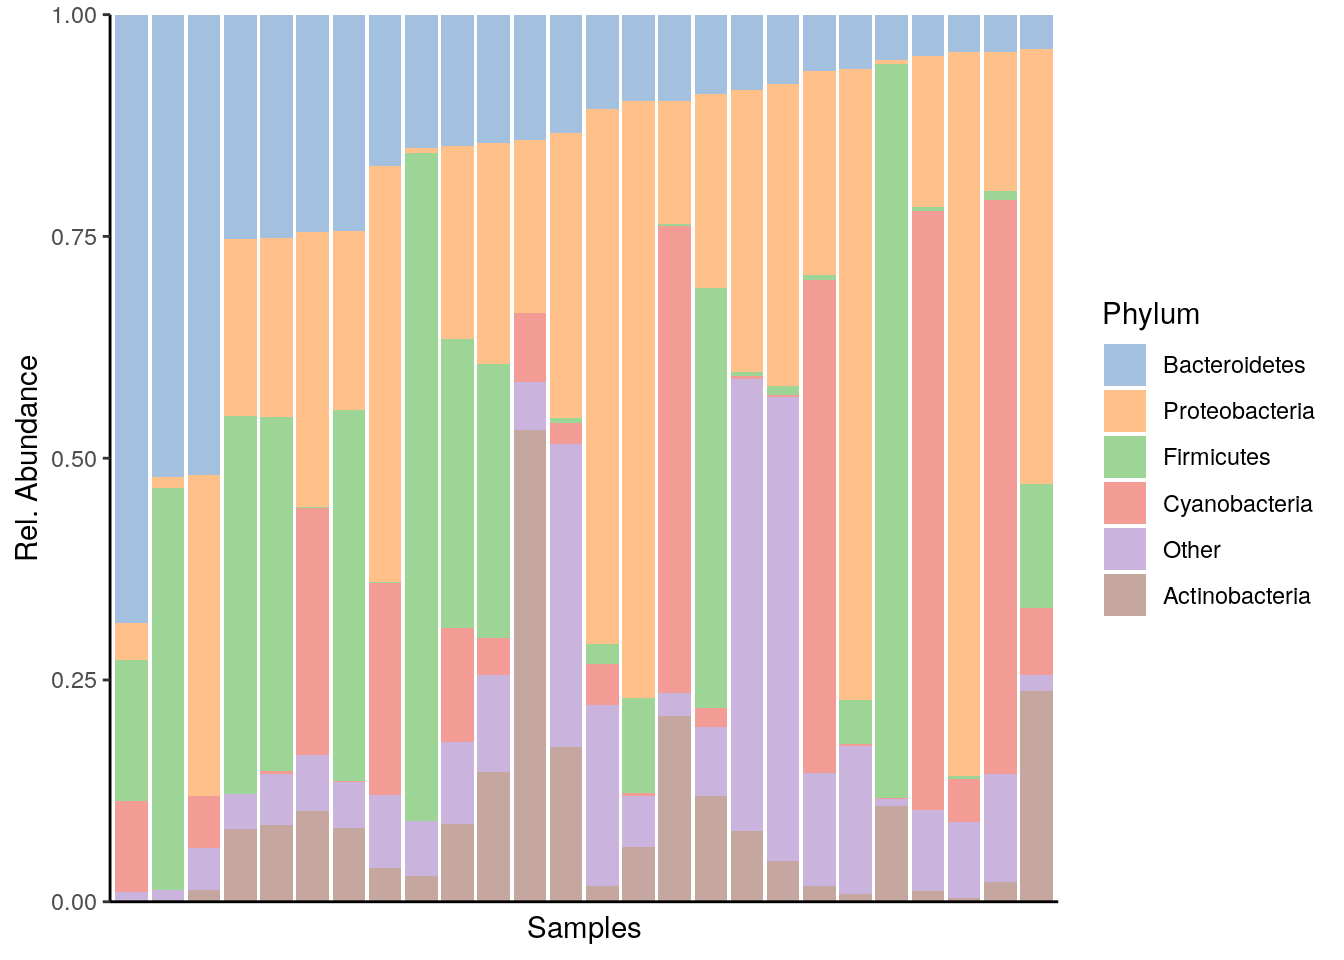
\includegraphics{21_microbiome_community_files/figure-latex/unnamed-chunk-1-1.pdf}

\hypertarget{composition-heatmap}{%
\subsection{Composition heatmap}\label{composition-heatmap}}

Community composition can be visualized with heatmap, where the
horizontal axis represents samples and the vertical axis the
taxa. Color of each intersection point represents abundance of a taxon
in a specific sample.

Here, abundances are first CLR (centered log-ratio) transformed to
remove compositionality bias. Then Z transformation is applied to
CLR-transformed data. This shifts all taxa to zero mean and unit
variance, allowing visual comparison between taxa that have different
absolute abundance levels. After these rough visual exploration
techniques, we can visualize the abundances at Phylum level.

\begin{Shaded}
\begin{Highlighting}[]
\FunctionTok{library}\NormalTok{(ggplot2)}
\CommentTok{\# Add clr{-}transformation on samples}
\NormalTok{tse\_phylum }\OtherTok{\textless{}{-}} \FunctionTok{transformSamples}\NormalTok{(tse\_phylum, }\AttributeTok{method =} \StringTok{"clr"}\NormalTok{, }\AttributeTok{pseudocount =} \DecValTok{1}\NormalTok{)}
\CommentTok{\# Add z{-}transformation on features (taxa)}
\NormalTok{tse\_phylum }\OtherTok{\textless{}{-}} \FunctionTok{transformFeatures}\NormalTok{(tse\_phylum, }\AttributeTok{abund\_values =} \StringTok{"clr"}\NormalTok{, }
                                \AttributeTok{method =} \StringTok{"z"}\NormalTok{, }\AttributeTok{name =} \StringTok{"clr\_z"}\NormalTok{)}
\CommentTok{\# Melts the assay}
\NormalTok{df }\OtherTok{\textless{}{-}} \FunctionTok{meltAssay}\NormalTok{(tse\_phylum, }\AttributeTok{abund\_values =} \StringTok{"clr\_z"}\NormalTok{)}

\CommentTok{\# Determines the scaling of colours}
\NormalTok{maxval }\OtherTok{\textless{}{-}} \FunctionTok{round}\NormalTok{(}\FunctionTok{max}\NormalTok{(}\FunctionTok{abs}\NormalTok{(df}\SpecialCharTok{$}\NormalTok{clr\_z)))}
\NormalTok{limits }\OtherTok{\textless{}{-}} \FunctionTok{c}\NormalTok{(}\SpecialCharTok{{-}}\NormalTok{maxval, maxval)}
\NormalTok{breaks }\OtherTok{\textless{}{-}} \FunctionTok{seq}\NormalTok{(}\AttributeTok{from =} \FunctionTok{min}\NormalTok{(limits), }\AttributeTok{to =} \FunctionTok{max}\NormalTok{(limits), }\AttributeTok{by =} \FloatTok{0.5}\NormalTok{)}
\NormalTok{colours }\OtherTok{\textless{}{-}} \FunctionTok{c}\NormalTok{(}\StringTok{"darkblue"}\NormalTok{, }\StringTok{"blue"}\NormalTok{, }\StringTok{"white"}\NormalTok{, }\StringTok{"red"}\NormalTok{, }\StringTok{"darkred"}\NormalTok{)}

\CommentTok{\# Creates a ggplot object}
\FunctionTok{ggplot}\NormalTok{(df, }\FunctionTok{aes}\NormalTok{(}\AttributeTok{x =}\NormalTok{ SampleID, }\AttributeTok{y =}\NormalTok{ FeatureID, }\AttributeTok{fill =}\NormalTok{ clr\_z)) }\SpecialCharTok{+}
  \FunctionTok{geom\_tile}\NormalTok{() }\SpecialCharTok{+}
  \FunctionTok{scale\_fill\_gradientn}\NormalTok{(}\AttributeTok{name =} \StringTok{"CLR + Z transform"}\NormalTok{, }
                       \AttributeTok{breaks =}\NormalTok{ breaks, }\AttributeTok{limits =}\NormalTok{ limits, }\AttributeTok{colours =}\NormalTok{ colours) }\SpecialCharTok{+} 
  \FunctionTok{theme}\NormalTok{(}\AttributeTok{text =} \FunctionTok{element\_text}\NormalTok{(}\AttributeTok{size=}\DecValTok{10}\NormalTok{),}
        \AttributeTok{axis.text.x =} \FunctionTok{element\_text}\NormalTok{(}\AttributeTok{angle=}\DecValTok{45}\NormalTok{, }\AttributeTok{hjust=}\DecValTok{1}\NormalTok{),}
        \AttributeTok{legend.key.size =} \FunctionTok{unit}\NormalTok{(}\DecValTok{1}\NormalTok{, }\StringTok{"cm"}\NormalTok{)) }\SpecialCharTok{+}
  \FunctionTok{labs}\NormalTok{(}\AttributeTok{x =} \StringTok{"Samples"}\NormalTok{, }\AttributeTok{y =} \StringTok{"Taxa"}\NormalTok{)}
\end{Highlighting}
\end{Shaded}

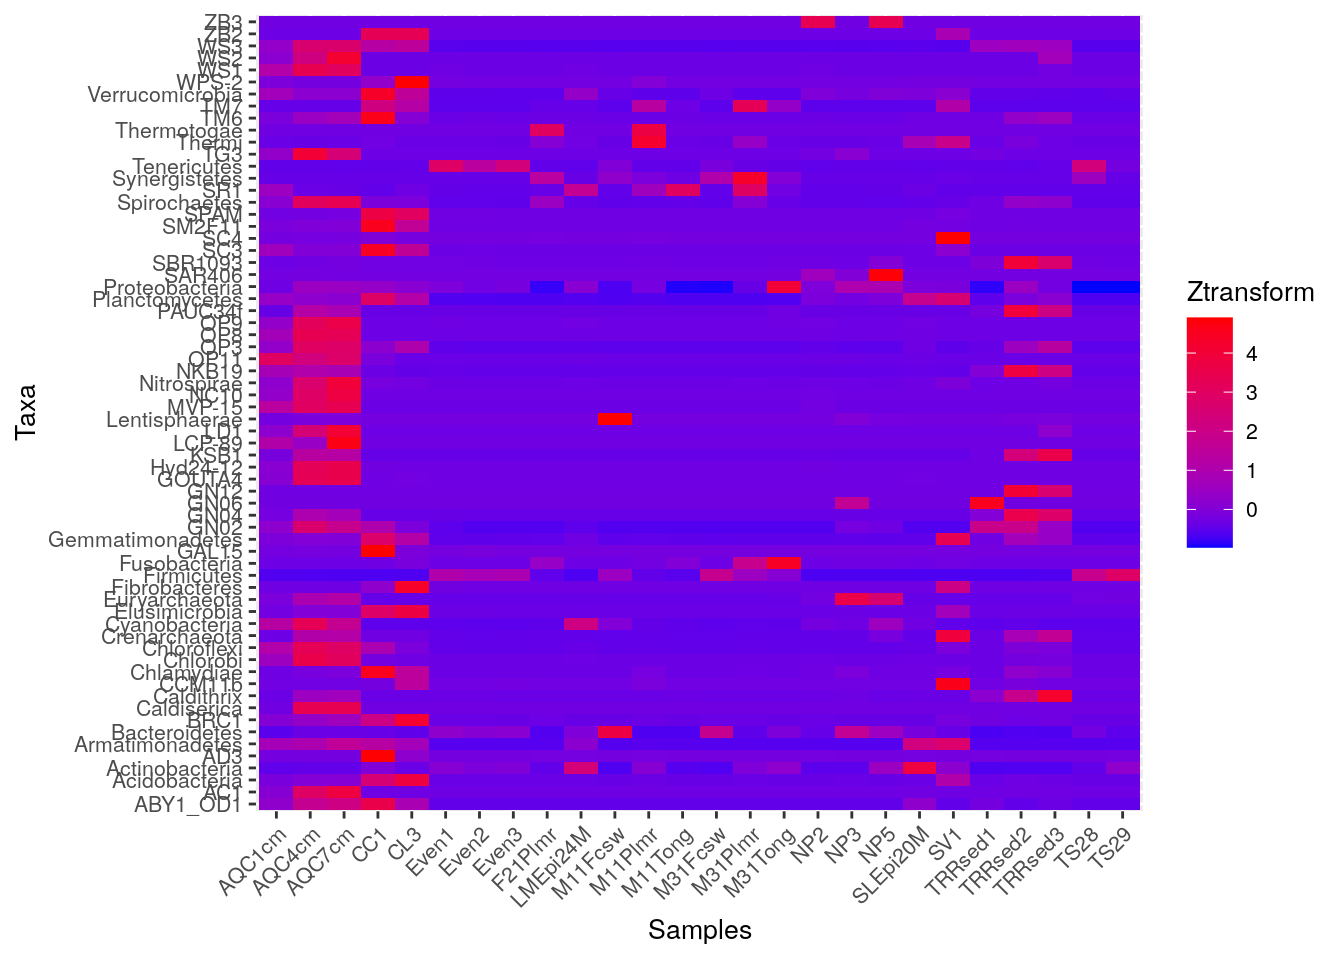
\includegraphics{21_microbiome_community_files/figure-latex/heatmap-1.pdf}

\emph{pheatmap} is a package that provides methods to plot clustered heatmaps.

\begin{Shaded}
\begin{Highlighting}[]
\ControlFlowTok{if}\NormalTok{(}\SpecialCharTok{!}\FunctionTok{require}\NormalTok{(pheatmap))\{}
  \FunctionTok{install.packages}\NormalTok{(}\StringTok{"pheatmap"}\NormalTok{)}
  \FunctionTok{library}\NormalTok{(pheatmap)}
\NormalTok{\}}

\CommentTok{\# Takes subset: only samples from feces, skin, or tongue}
\NormalTok{tse\_phylum\_subset }\OtherTok{\textless{}{-}}\NormalTok{ tse\_phylum[ , }\FunctionTok{colData}\NormalTok{(tse\_phylum)}\SpecialCharTok{$}\NormalTok{SampleType }\SpecialCharTok{\%in\%} \FunctionTok{c}\NormalTok{(}\StringTok{"Feces"}\NormalTok{, }\StringTok{"Skin"}\NormalTok{, }\StringTok{"Tongue"}\NormalTok{) ]}

\CommentTok{\# Does clr{-}transformation}
\NormalTok{tse\_phylum\_subset }\OtherTok{\textless{}{-}} \FunctionTok{transformSamples}\NormalTok{(tse\_phylum\_subset, }\AttributeTok{method =} \StringTok{"clr"}\NormalTok{, }\AttributeTok{pseudocount =} \DecValTok{1}\NormalTok{)}
\CommentTok{\# Does z{-}transformation}
\NormalTok{tse\_phylum\_subset }\OtherTok{\textless{}{-}} \FunctionTok{transformFeatures}\NormalTok{(tse\_phylum\_subset, }\AttributeTok{abund\_values =} \StringTok{"clr"}\NormalTok{, }
                                       \AttributeTok{method =} \StringTok{"z"}\NormalTok{, }\AttributeTok{name =} \StringTok{"clr\_z"}\NormalTok{)}

\CommentTok{\# Get n most abundant taxa, and subsets the data by them}
\NormalTok{top\_taxa }\OtherTok{\textless{}{-}} \FunctionTok{getTopTaxa}\NormalTok{(tse\_phylum\_subset, }\AttributeTok{top =} \DecValTok{20}\NormalTok{)}
\NormalTok{tse\_phylum\_subset }\OtherTok{\textless{}{-}}\NormalTok{ tse\_phylum\_subset[top\_taxa, ]}

\CommentTok{\# Gets the assay table}
\NormalTok{mat }\OtherTok{\textless{}{-}} \FunctionTok{assay}\NormalTok{(tse\_phylum\_subset, }\StringTok{"clr\_z"}\NormalTok{)}

\CommentTok{\# Creates the heatmap}
\FunctionTok{pheatmap}\NormalTok{(mat)}
\end{Highlighting}
\end{Shaded}

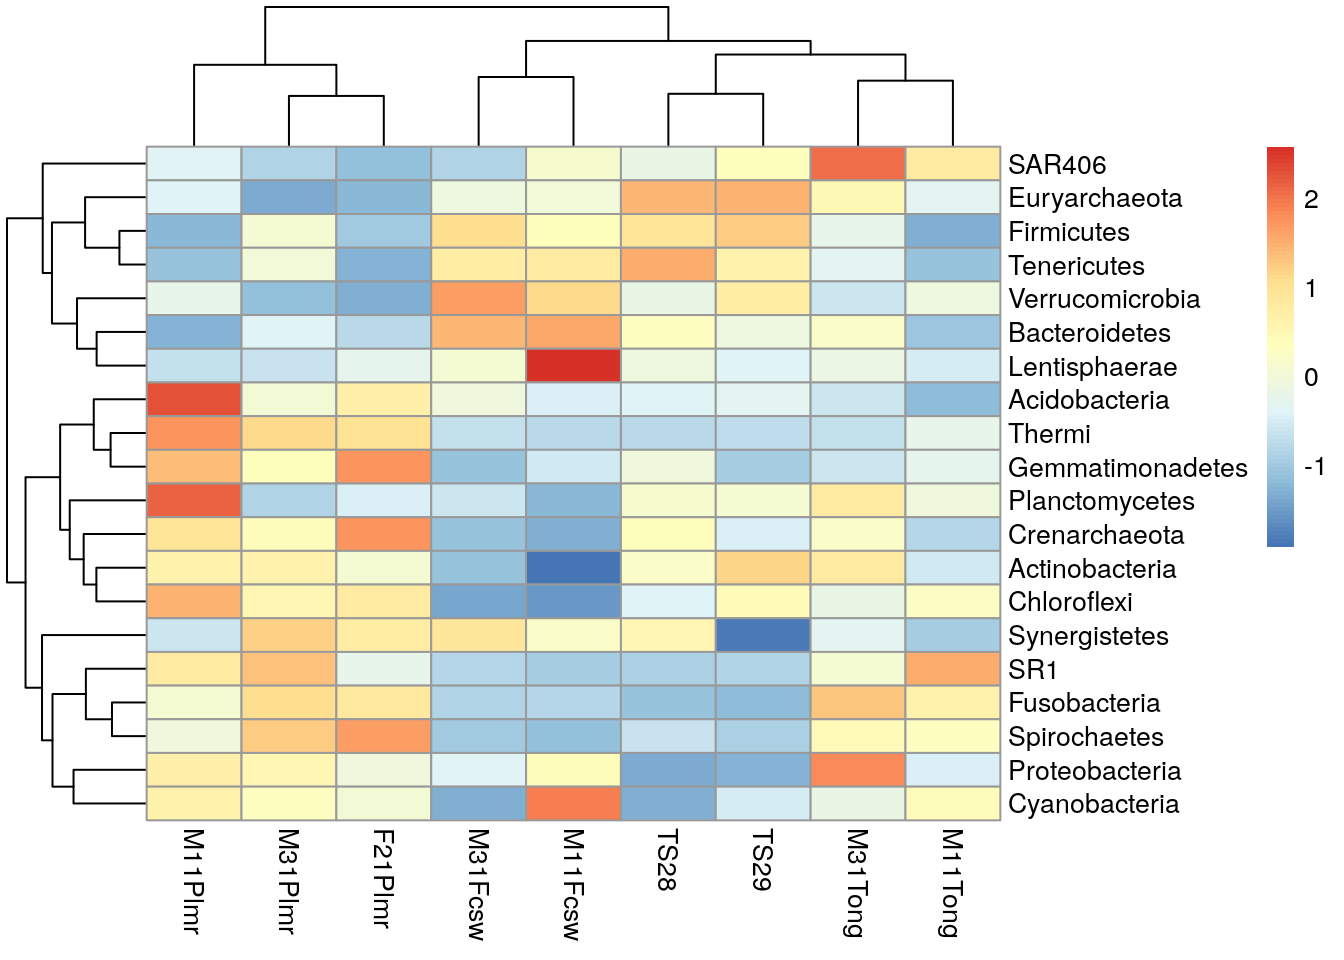
\includegraphics{21_microbiome_community_files/figure-latex/pheatmap1-1.pdf}

We can create clusters by hierarchical clustering and add them to the plot.

\begin{Shaded}
\begin{Highlighting}[]
\ControlFlowTok{if}\NormalTok{(}\SpecialCharTok{!}\FunctionTok{require}\NormalTok{(ape))\{}
    \FunctionTok{install.packages}\NormalTok{(}\StringTok{"ape"}\NormalTok{)}
    \FunctionTok{library}\NormalTok{(ape)}
\NormalTok{\}}

\CommentTok{\# Hierarchical clustering}
\NormalTok{taxa\_hclust }\OtherTok{\textless{}{-}} \FunctionTok{hclust}\NormalTok{(}\FunctionTok{dist}\NormalTok{(mat), }\AttributeTok{method =} \StringTok{"complete"}\NormalTok{)}

\CommentTok{\# Creates a phylogenetic tree}
\NormalTok{taxa\_tree }\OtherTok{\textless{}{-}} \FunctionTok{as.phylo}\NormalTok{(taxa\_hclust)}
\end{Highlighting}
\end{Shaded}

\begin{Shaded}
\begin{Highlighting}[]
\ControlFlowTok{if}\NormalTok{(}\SpecialCharTok{!}\FunctionTok{require}\NormalTok{(ggtree))\{}
    \FunctionTok{install.packages}\NormalTok{(}\StringTok{"ggtree"}\NormalTok{)}
    \FunctionTok{library}\NormalTok{(ggtree)}
\NormalTok{\}}

\CommentTok{\# Plot taxa tree}
\NormalTok{taxa\_tree }\OtherTok{\textless{}{-}} \FunctionTok{ggtree}\NormalTok{(taxa\_tree) }\SpecialCharTok{+} 
  \FunctionTok{theme}\NormalTok{(}\AttributeTok{plot.margin=}\FunctionTok{margin}\NormalTok{(}\DecValTok{0}\NormalTok{,}\DecValTok{0}\NormalTok{,}\DecValTok{0}\NormalTok{,}\DecValTok{0}\NormalTok{)) }\CommentTok{\# removes margins}

\CommentTok{\# Get order of taxa in plot}
\NormalTok{taxa\_ordered }\OtherTok{\textless{}{-}} \FunctionTok{get\_taxa\_name}\NormalTok{(taxa\_tree)}

\NormalTok{taxa\_tree}
\end{Highlighting}
\end{Shaded}

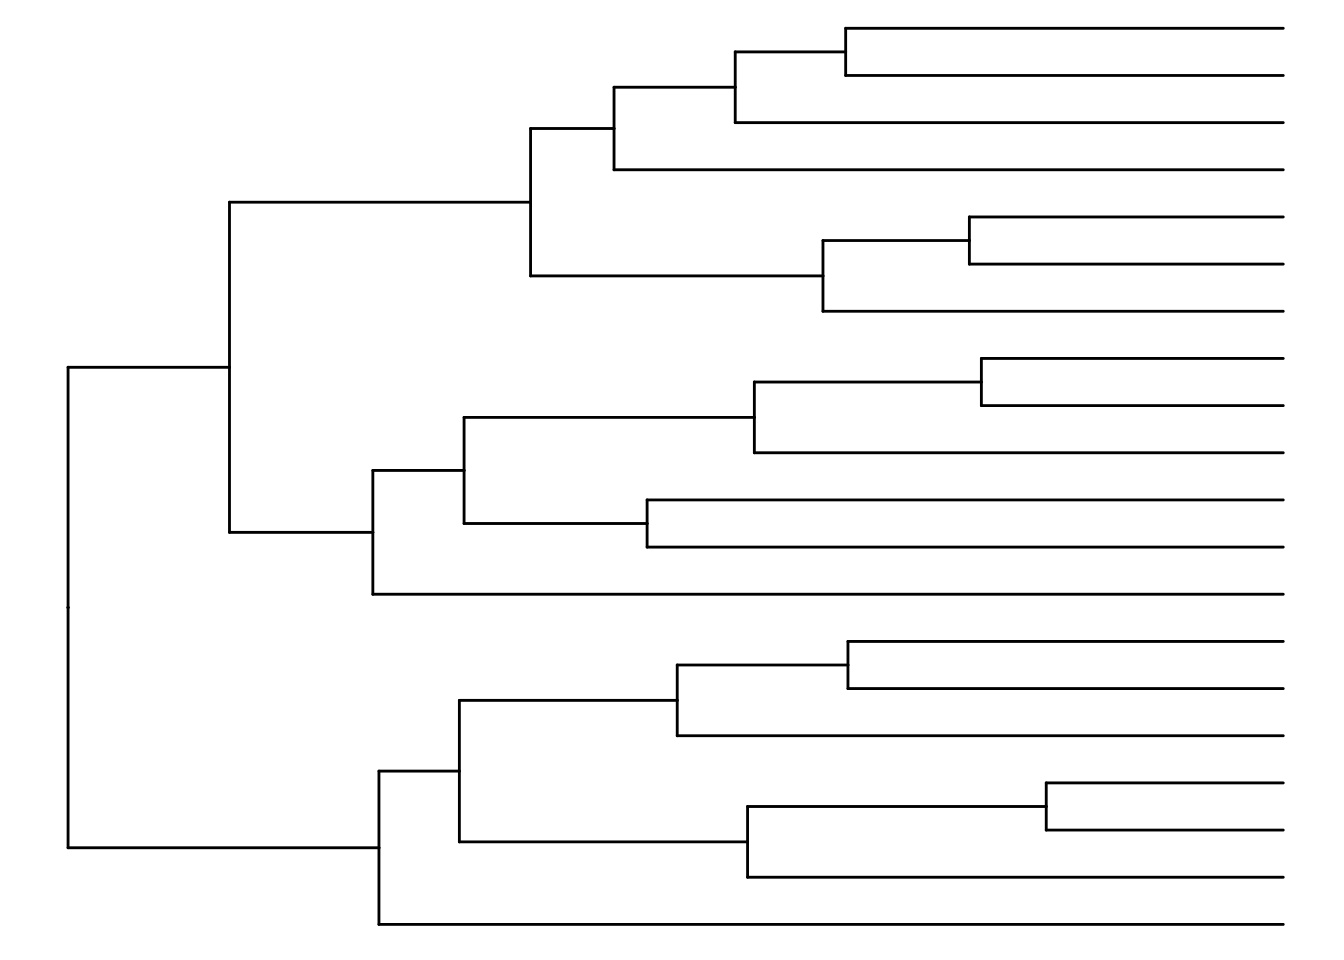
\includegraphics{21_microbiome_community_files/figure-latex/pheatmap3-1.pdf}

Based on phylo tree, we decide to create three clusters.

\begin{Shaded}
\begin{Highlighting}[]
\CommentTok{\# Creates clusters}
\NormalTok{taxa\_clusters }\OtherTok{\textless{}{-}} \FunctionTok{cutree}\NormalTok{(}\AttributeTok{tree =}\NormalTok{ taxa\_hclust, }\AttributeTok{k =} \DecValTok{3}\NormalTok{)}

\CommentTok{\# Converts into data frame}
\NormalTok{taxa\_clusters }\OtherTok{\textless{}{-}} \FunctionTok{data.frame}\NormalTok{(}\AttributeTok{clusters =}\NormalTok{ taxa\_clusters)}
\NormalTok{taxa\_clusters}\SpecialCharTok{$}\NormalTok{clusters }\OtherTok{\textless{}{-}} \FunctionTok{factor}\NormalTok{(taxa\_clusters}\SpecialCharTok{$}\NormalTok{clusters)}

\CommentTok{\# Order data so that it\textquotesingle{}s same as in phylo tree}
\NormalTok{taxa\_clusters }\OtherTok{\textless{}{-}}\NormalTok{ taxa\_clusters[taxa\_ordered, , drop }\OtherTok{=} \ConstantTok{FALSE}\NormalTok{] }

\CommentTok{\# Prints taxa and their clusters}
\NormalTok{taxa\_clusters}
\end{Highlighting}
\end{Shaded}

\begin{verbatim}
##                  clusters
## Chloroflexi             3
## Actinobacteria          3
## Crenarchaeota           3
## Planctomycetes          3
## Gemmatimonadetes        3
## Thermi                  3
## Acidobacteria           3
## Spirochaetes            2
## Fusobacteria            2
## SR1                     2
## Cyanobacteria           2
## Proteobacteria          2
## Synergistetes           2
## Lentisphaerae           1
## Bacteroidetes           1
## Verrucomicrobia         1
## Tenericutes             1
## Firmicutes              1
## Euryarchaeota           1
## SAR406                  1
\end{verbatim}

\begin{Shaded}
\begin{Highlighting}[]
\CommentTok{\# Adds information to rowData}
\FunctionTok{rowData}\NormalTok{(tse\_phylum\_subset)}\SpecialCharTok{$}\NormalTok{clusters }\OtherTok{\textless{}{-}}\NormalTok{ taxa\_clusters[}\FunctionTok{order}\NormalTok{(}\FunctionTok{match}\NormalTok{(}\FunctionTok{rownames}\NormalTok{(taxa\_clusters), }
                                                                 \FunctionTok{rownames}\NormalTok{(tse\_phylum\_subset))), ]}

\CommentTok{\# Prints taxa and their clusters}
\FunctionTok{rowData}\NormalTok{(tse\_phylum\_subset)}\SpecialCharTok{$}\NormalTok{clusters}
\end{Highlighting}
\end{Shaded}

\begin{verbatim}
##  [1] 1 1 2 3 2 2 1 1 1 1 3 2 3 3 3 2 2 3 3 1
## Levels: 1 2 3
\end{verbatim}

\begin{Shaded}
\begin{Highlighting}[]
\CommentTok{\# Hierarchical clustering}
\NormalTok{sample\_hclust }\OtherTok{\textless{}{-}} \FunctionTok{hclust}\NormalTok{(}\FunctionTok{dist}\NormalTok{(}\FunctionTok{t}\NormalTok{(mat)), }\AttributeTok{method =} \StringTok{"complete"}\NormalTok{)}

\CommentTok{\# Creates a phylogenetic tree}
\NormalTok{sample\_tree }\OtherTok{\textless{}{-}} \FunctionTok{as.phylo}\NormalTok{(sample\_hclust)}

\CommentTok{\# Plot sample tree}
\NormalTok{sample\_tree }\OtherTok{\textless{}{-}} \FunctionTok{ggtree}\NormalTok{(sample\_tree) }\SpecialCharTok{+} \FunctionTok{layout\_dendrogram}\NormalTok{() }\SpecialCharTok{+} 
  \FunctionTok{theme}\NormalTok{(}\AttributeTok{plot.margin=}\FunctionTok{margin}\NormalTok{(}\DecValTok{0}\NormalTok{,}\DecValTok{0}\NormalTok{,}\DecValTok{0}\NormalTok{,}\DecValTok{0}\NormalTok{)) }\CommentTok{\# removes margins}

\CommentTok{\# Get order of samples in plot}
\NormalTok{samples\_ordered }\OtherTok{\textless{}{-}} \FunctionTok{rev}\NormalTok{(}\FunctionTok{get\_taxa\_name}\NormalTok{(sample\_tree))}

\NormalTok{sample\_tree}
\end{Highlighting}
\end{Shaded}

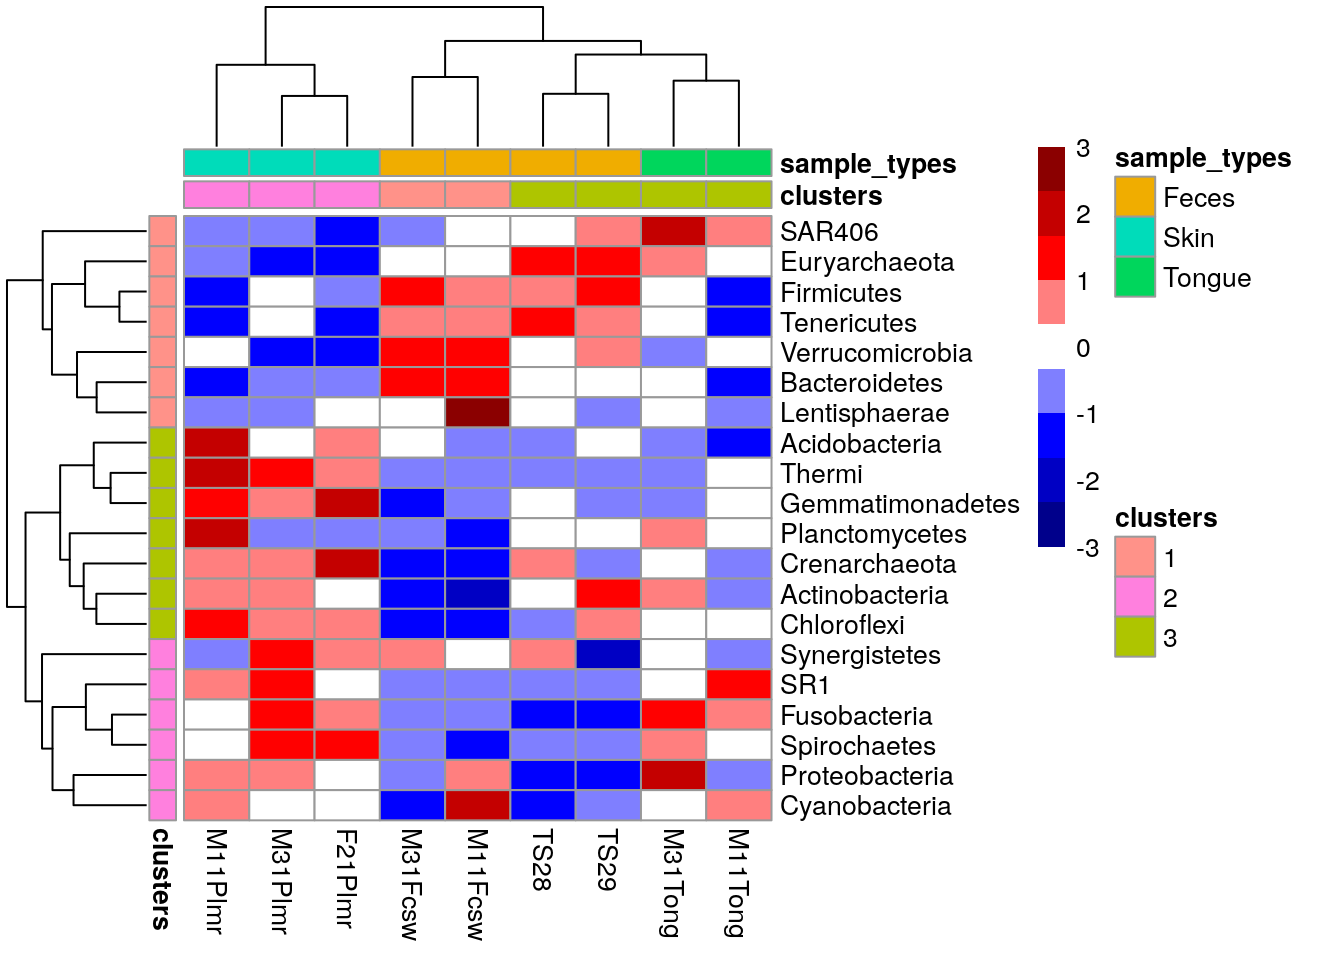
\includegraphics{21_microbiome_community_files/figure-latex/pheatmap6-1.pdf}

\begin{Shaded}
\begin{Highlighting}[]
\CommentTok{\# Creates clusters}
\NormalTok{sample\_clusters }\OtherTok{\textless{}{-}} \FunctionTok{factor}\NormalTok{(}\FunctionTok{cutree}\NormalTok{(}\AttributeTok{tree =}\NormalTok{ sample\_hclust, }\AttributeTok{k =} \DecValTok{3}\NormalTok{))}

\CommentTok{\# Converts into data frame}
\NormalTok{sample\_data }\OtherTok{\textless{}{-}} \FunctionTok{data.frame}\NormalTok{(}\AttributeTok{clusters =}\NormalTok{ sample\_clusters)}

\CommentTok{\# Order data so that it\textquotesingle{}s same as in phylo tree}
\NormalTok{sample\_data }\OtherTok{\textless{}{-}}\NormalTok{ sample\_data[samples\_ordered, , drop }\OtherTok{=} \ConstantTok{FALSE}\NormalTok{] }

\CommentTok{\# Order data based on }
\NormalTok{tse\_phylum\_subset }\OtherTok{\textless{}{-}}\NormalTok{ tse\_phylum\_subset[ , }\FunctionTok{rownames}\NormalTok{(sample\_data)]}

\CommentTok{\# Add sample type data}
\NormalTok{sample\_data}\SpecialCharTok{$}\NormalTok{sample\_types }\OtherTok{\textless{}{-}} \FunctionTok{unfactor}\NormalTok{(}\FunctionTok{colData}\NormalTok{(tse\_phylum\_subset)}\SpecialCharTok{$}\NormalTok{SampleType)}

\NormalTok{sample\_data}
\end{Highlighting}
\end{Shaded}

\begin{verbatim}
##         clusters sample_types
## M11Plmr        2         Skin
## M31Plmr        2         Skin
## F21Plmr        2         Skin
## M31Fcsw        1        Feces
## M11Fcsw        1        Feces
## TS28           3        Feces
## TS29           3        Feces
## M31Tong        3       Tongue
## M11Tong        3       Tongue
\end{verbatim}

Now we can create heatmap with additional annotations.

\begin{Shaded}
\begin{Highlighting}[]
\CommentTok{\# Determines the scaling of colorss}
\CommentTok{\# Scale colors}
\NormalTok{breaks }\OtherTok{\textless{}{-}} \FunctionTok{seq}\NormalTok{(}\SpecialCharTok{{-}}\FunctionTok{ceiling}\NormalTok{(}\FunctionTok{max}\NormalTok{(}\FunctionTok{abs}\NormalTok{(mat))), }\FunctionTok{ceiling}\NormalTok{(}\FunctionTok{max}\NormalTok{(}\FunctionTok{abs}\NormalTok{(mat))), }
              \AttributeTok{length.out =} \FunctionTok{ifelse}\NormalTok{( }\FunctionTok{max}\NormalTok{(}\FunctionTok{abs}\NormalTok{(mat))}\SpecialCharTok{\textgreater{}}\DecValTok{5}\NormalTok{, }\DecValTok{2}\SpecialCharTok{*}\FunctionTok{ceiling}\NormalTok{(}\FunctionTok{max}\NormalTok{(}\FunctionTok{abs}\NormalTok{(mat))), }\DecValTok{10}\NormalTok{ ) )}
\NormalTok{colors }\OtherTok{\textless{}{-}} \FunctionTok{colorRampPalette}\NormalTok{(}\FunctionTok{c}\NormalTok{(}\StringTok{"darkblue"}\NormalTok{, }\StringTok{"blue"}\NormalTok{, }\StringTok{"white"}\NormalTok{, }\StringTok{"red"}\NormalTok{, }\StringTok{"darkred"}\NormalTok{))(}\FunctionTok{length}\NormalTok{(breaks)}\SpecialCharTok{{-}}\DecValTok{1}\NormalTok{)}

\FunctionTok{pheatmap}\NormalTok{(mat, }\AttributeTok{annotation\_row =}\NormalTok{ taxa\_clusters, }
         \AttributeTok{annotation\_col =}\NormalTok{ sample\_data,}
         \AttributeTok{breaks =}\NormalTok{ breaks,}
         \AttributeTok{color =}\NormalTok{ colors)}
\end{Highlighting}
\end{Shaded}

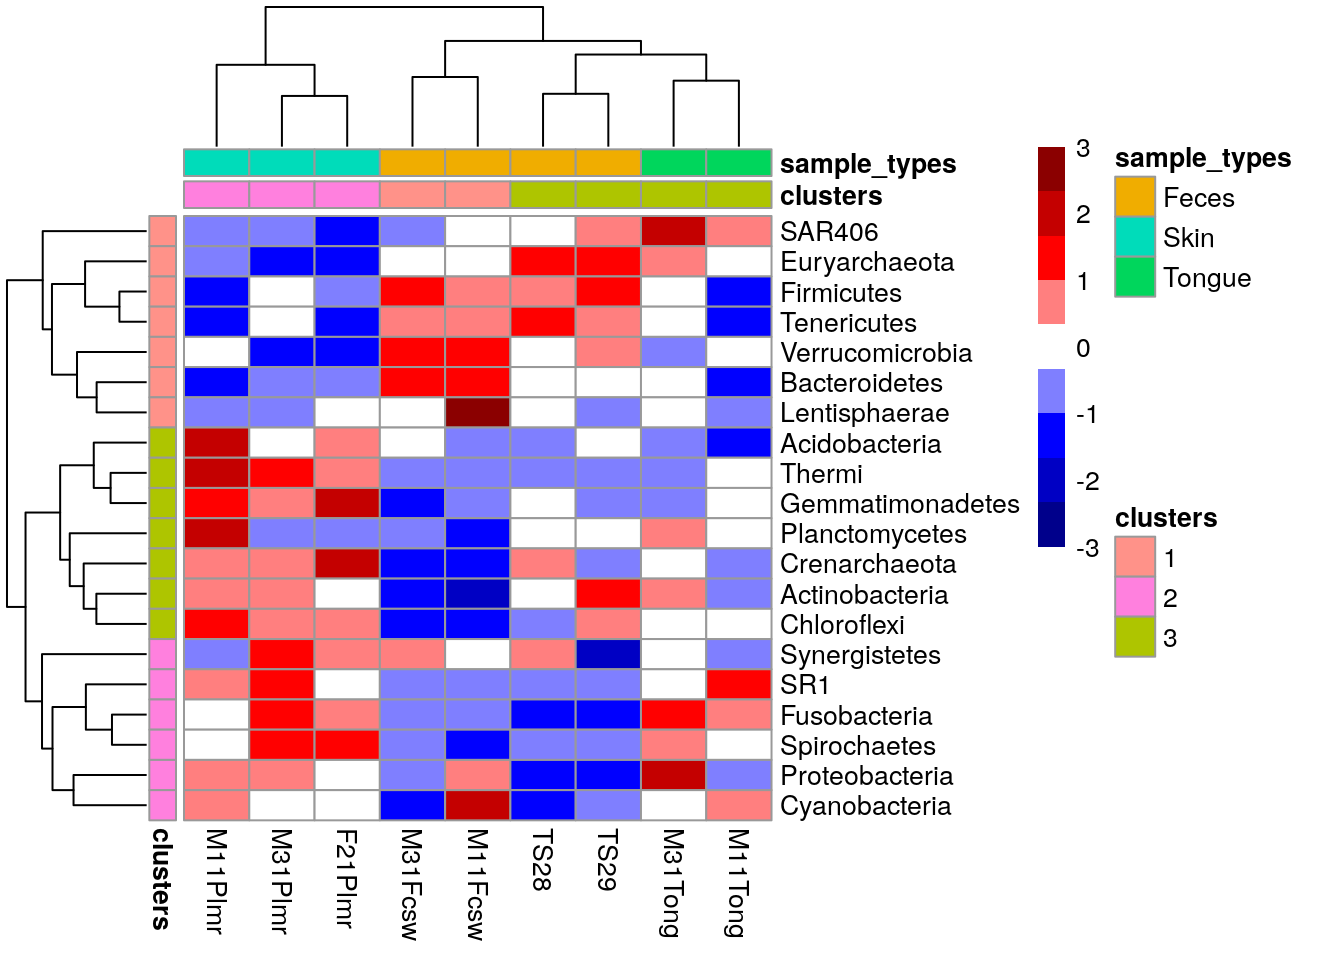
\includegraphics{21_microbiome_community_files/figure-latex/pheatmap8-1.pdf}

In addition to \emph{pheatmap} package, there are also other packages that
provide functions for more complex heatmaps, such as \href{https://docs.ropensci.org/iheatmapr/articles/full_vignettes/iheatmapr.html}{\emph{iheatmapr}}
and
\href{https://academic.oup.com/bioinformatics/article/32/18/2847/1743594?login=true}{ComplexHeatmap}.

\href{http://www.bioconductor.org/packages/release/bioc/vignettes/sechm/inst/doc/sechm.html}{sechm}
package provides wrapper for \emph{ComplexHeatmap}.

\begin{Shaded}
\begin{Highlighting}[]
\ControlFlowTok{if}\NormalTok{(}\SpecialCharTok{!}\FunctionTok{require}\NormalTok{(sechm))\{}
\NormalTok{  BiocManager}\SpecialCharTok{::}\FunctionTok{install}\NormalTok{(}\StringTok{"sechm"}\NormalTok{)}
  \FunctionTok{library}\NormalTok{(sechm)}
\NormalTok{\}}
\CommentTok{\# Stores annotation colros to metadata}
\FunctionTok{metadata}\NormalTok{(tse\_phylum\_subset)}\SpecialCharTok{$}\NormalTok{anno\_colors}\SpecialCharTok{$}\NormalTok{SampleType }\OtherTok{\textless{}{-}} \FunctionTok{c}\NormalTok{(}\AttributeTok{Feces =} \StringTok{"blue"}\NormalTok{, }
                                                        \AttributeTok{Skin =} \StringTok{"red"}\NormalTok{, }
                                                        \AttributeTok{Tongue =} \StringTok{"gray"}\NormalTok{)}

\CommentTok{\# Create a plot}
\FunctionTok{sechm}\NormalTok{(tse\_phylum\_subset, }
      \AttributeTok{genes =} \FunctionTok{rownames}\NormalTok{(tse\_phylum\_subset), }
      \AttributeTok{assayName =} \StringTok{"clr"}\NormalTok{, }
      \AttributeTok{do.scale =} \ConstantTok{TRUE}\NormalTok{, }
      \AttributeTok{top\_annotation =} \FunctionTok{c}\NormalTok{(}\StringTok{"SampleType"}\NormalTok{), }
      \AttributeTok{gaps\_at =} \StringTok{"SampleType"}\NormalTok{,}
      \AttributeTok{cluster\_cols =} \ConstantTok{TRUE}\NormalTok{, }\AttributeTok{cluster\_rows =} \ConstantTok{TRUE}\NormalTok{)}
\end{Highlighting}
\end{Shaded}

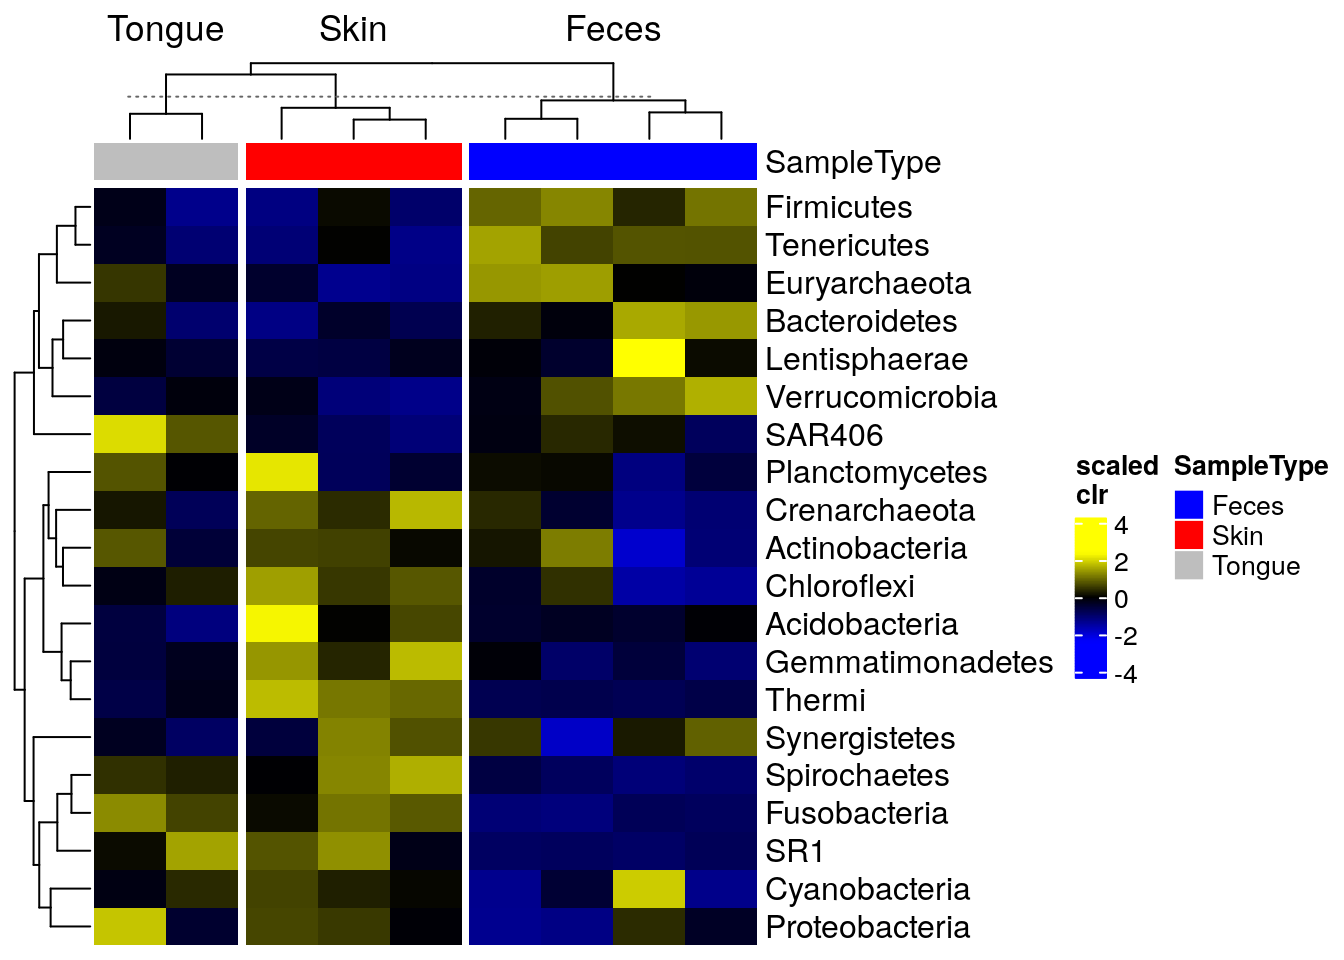
\includegraphics{21_microbiome_community_files/figure-latex/sechm-1.pdf}

It is also possible to create similar heatmap by just using \emph{ggplot2}.

\begin{Shaded}
\begin{Highlighting}[]
\CommentTok{\# Add feature names to column as a factor}
\NormalTok{taxa\_clusters}\SpecialCharTok{$}\NormalTok{Feature }\OtherTok{\textless{}{-}} \FunctionTok{rownames}\NormalTok{(taxa\_clusters)}
\NormalTok{taxa\_clusters}\SpecialCharTok{$}\NormalTok{Feature }\OtherTok{\textless{}{-}} \FunctionTok{factor}\NormalTok{(taxa\_clusters}\SpecialCharTok{$}\NormalTok{Feature, }\AttributeTok{levels =}\NormalTok{ taxa\_clusters}\SpecialCharTok{$}\NormalTok{Feature)}

\CommentTok{\# Create annotation plot}
\NormalTok{row\_annotation }\OtherTok{\textless{}{-}} \FunctionTok{ggplot}\NormalTok{(taxa\_clusters) }\SpecialCharTok{+} 
  \FunctionTok{geom\_tile}\NormalTok{(}\FunctionTok{aes}\NormalTok{(}\AttributeTok{x =} \ConstantTok{NA}\NormalTok{, }\AttributeTok{y =}\NormalTok{ Feature, }\AttributeTok{fill =}\NormalTok{ clusters)) }\SpecialCharTok{+} \FunctionTok{coord\_equal}\NormalTok{(}\AttributeTok{ratio =} \DecValTok{1}\NormalTok{) }\SpecialCharTok{+}
  \FunctionTok{theme}\NormalTok{(}
        \AttributeTok{axis.text.x=}\FunctionTok{element\_blank}\NormalTok{(),}
        \AttributeTok{axis.text.y=}\FunctionTok{element\_blank}\NormalTok{(),}
        \AttributeTok{axis.ticks.y=}\FunctionTok{element\_blank}\NormalTok{(),}
        \AttributeTok{axis.title.y=}\FunctionTok{element\_blank}\NormalTok{(),}
        \AttributeTok{axis.title.x =} \FunctionTok{element\_text}\NormalTok{(}\AttributeTok{angle =} \DecValTok{90}\NormalTok{, }\AttributeTok{vjust =} \FloatTok{0.5}\NormalTok{, }\AttributeTok{hjust=}\DecValTok{1}\NormalTok{),}
        \AttributeTok{plot.margin=}\FunctionTok{margin}\NormalTok{(}\DecValTok{0}\NormalTok{,}\DecValTok{0}\NormalTok{,}\DecValTok{0}\NormalTok{,}\DecValTok{0}\NormalTok{),}
\NormalTok{        ) }\SpecialCharTok{+}
      \FunctionTok{labs}\NormalTok{(}\AttributeTok{fill =} \StringTok{"Clusters"}\NormalTok{, }\AttributeTok{x =} \StringTok{"Clusters"}\NormalTok{)}

\NormalTok{row\_annotation}
\end{Highlighting}
\end{Shaded}

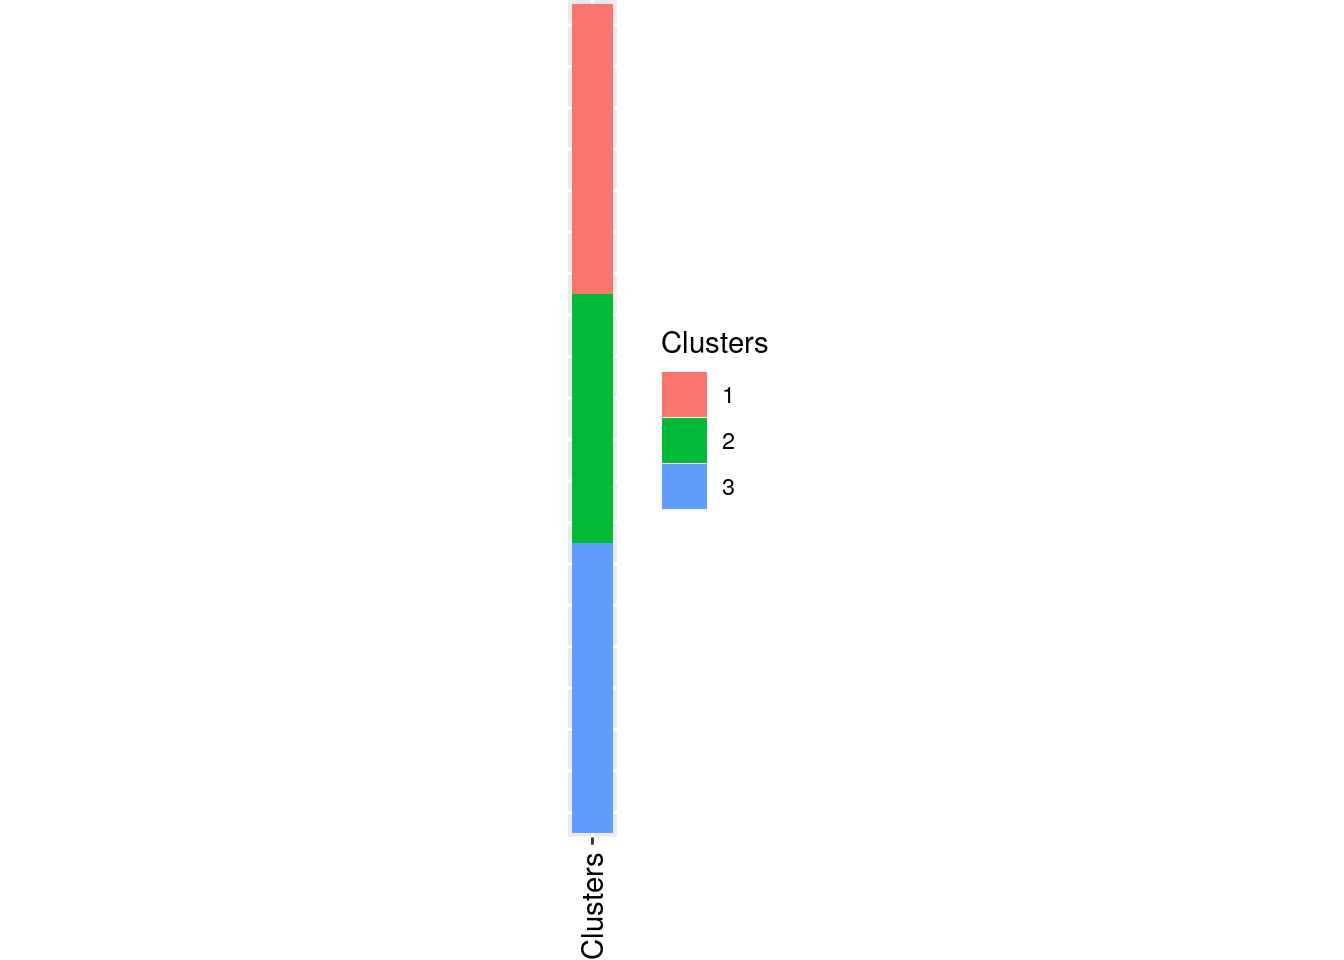
\includegraphics{21_microbiome_community_files/figure-latex/more_complex_heatmap1-1.pdf}

\begin{Shaded}
\begin{Highlighting}[]
\CommentTok{\# Add sample names to one of the columns}
\NormalTok{sample\_data}\SpecialCharTok{$}\NormalTok{sample }\OtherTok{\textless{}{-}} \FunctionTok{factor}\NormalTok{(}\FunctionTok{rownames}\NormalTok{(sample\_data), }\AttributeTok{levels =} \FunctionTok{rownames}\NormalTok{(sample\_data))}

\CommentTok{\# Create annotation plot}
\NormalTok{sample\_types\_annotation }\OtherTok{\textless{}{-}} \FunctionTok{ggplot}\NormalTok{(sample\_data) }\SpecialCharTok{+} \FunctionTok{scale\_y\_discrete}\NormalTok{(}\AttributeTok{position =} \StringTok{"right"}\NormalTok{, }\AttributeTok{expand =} \FunctionTok{c}\NormalTok{(}\DecValTok{0}\NormalTok{,}\DecValTok{0}\NormalTok{)) }\SpecialCharTok{+}
  \FunctionTok{geom\_tile}\NormalTok{(}\FunctionTok{aes}\NormalTok{(}\AttributeTok{y =} \ConstantTok{NA}\NormalTok{, }\AttributeTok{x =}\NormalTok{ sample, }\AttributeTok{fill =}\NormalTok{ sample\_types)) }\SpecialCharTok{+} \FunctionTok{coord\_equal}\NormalTok{(}\AttributeTok{ratio =} \DecValTok{1}\NormalTok{) }\SpecialCharTok{+}
  \FunctionTok{theme}\NormalTok{(}
        \AttributeTok{axis.text.x=}\FunctionTok{element\_blank}\NormalTok{(),}
        \AttributeTok{axis.text.y=}\FunctionTok{element\_blank}\NormalTok{(),}
        \AttributeTok{axis.title.x=}\FunctionTok{element\_blank}\NormalTok{(),}
        \AttributeTok{axis.ticks.x=}\FunctionTok{element\_blank}\NormalTok{(),}
        \AttributeTok{plot.margin=}\FunctionTok{margin}\NormalTok{(}\DecValTok{0}\NormalTok{,}\DecValTok{0}\NormalTok{,}\DecValTok{0}\NormalTok{,}\DecValTok{0}\NormalTok{),}
        \AttributeTok{axis.title.y.right =} \FunctionTok{element\_text}\NormalTok{(}\AttributeTok{angle=}\DecValTok{0}\NormalTok{, }\AttributeTok{vjust =} \FloatTok{0.5}\NormalTok{)}
\NormalTok{        ) }\SpecialCharTok{+}
      \FunctionTok{labs}\NormalTok{(}\AttributeTok{fill =} \StringTok{"Sample types"}\NormalTok{, }\AttributeTok{y =} \StringTok{"Sample types"}\NormalTok{)}

\NormalTok{sample\_types\_annotation}
\end{Highlighting}
\end{Shaded}

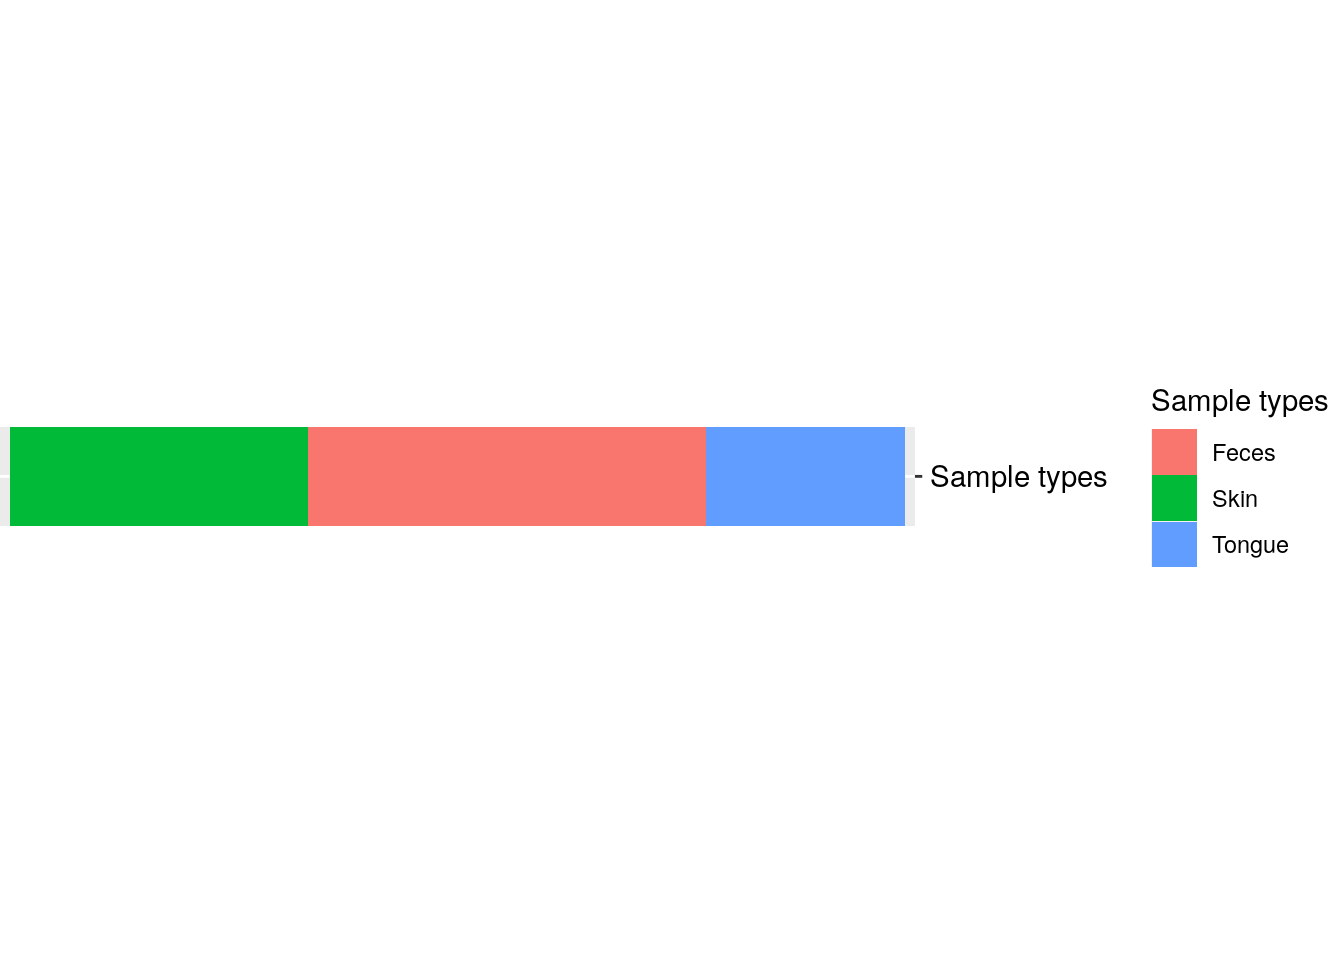
\includegraphics{21_microbiome_community_files/figure-latex/more_complex_heatmap2-1.pdf}

\begin{Shaded}
\begin{Highlighting}[]
\CommentTok{\# Create annotation plot}
\NormalTok{sample\_clusters\_annotation }\OtherTok{\textless{}{-}} \FunctionTok{ggplot}\NormalTok{(sample\_data) }\SpecialCharTok{+} \FunctionTok{scale\_y\_discrete}\NormalTok{(}\AttributeTok{position =} \StringTok{"right"}\NormalTok{, }\AttributeTok{expand =} \FunctionTok{c}\NormalTok{(}\DecValTok{0}\NormalTok{,}\DecValTok{0}\NormalTok{)) }\SpecialCharTok{+}
  \FunctionTok{geom\_tile}\NormalTok{(}\FunctionTok{aes}\NormalTok{(}\AttributeTok{y =} \ConstantTok{NA}\NormalTok{, }\AttributeTok{x =}\NormalTok{ sample, }\AttributeTok{fill =}\NormalTok{ clusters)) }\SpecialCharTok{+} \FunctionTok{coord\_equal}\NormalTok{(}\AttributeTok{ratio =} \DecValTok{1}\NormalTok{) }\SpecialCharTok{+}
  \FunctionTok{theme}\NormalTok{(}
        \AttributeTok{axis.text.x=}\FunctionTok{element\_blank}\NormalTok{(),}
        \AttributeTok{axis.text.y=}\FunctionTok{element\_blank}\NormalTok{(),}
        \AttributeTok{axis.title.x=}\FunctionTok{element\_blank}\NormalTok{(),}
        \AttributeTok{axis.ticks.x=}\FunctionTok{element\_blank}\NormalTok{(),}
        \AttributeTok{plot.margin=}\FunctionTok{margin}\NormalTok{(}\DecValTok{0}\NormalTok{,}\DecValTok{0}\NormalTok{,}\DecValTok{0}\NormalTok{,}\DecValTok{0}\NormalTok{),}
        \AttributeTok{axis.title.y.right =} \FunctionTok{element\_text}\NormalTok{(}\AttributeTok{angle=}\DecValTok{0}\NormalTok{, }\AttributeTok{vjust =} \FloatTok{0.5}\NormalTok{)}
\NormalTok{        ) }\SpecialCharTok{+}
      \FunctionTok{labs}\NormalTok{(}\AttributeTok{fill =} \StringTok{"Clusters"}\NormalTok{, }\AttributeTok{y =} \StringTok{"Clusters"}\NormalTok{)}

\NormalTok{sample\_clusters\_annotation}
\end{Highlighting}
\end{Shaded}

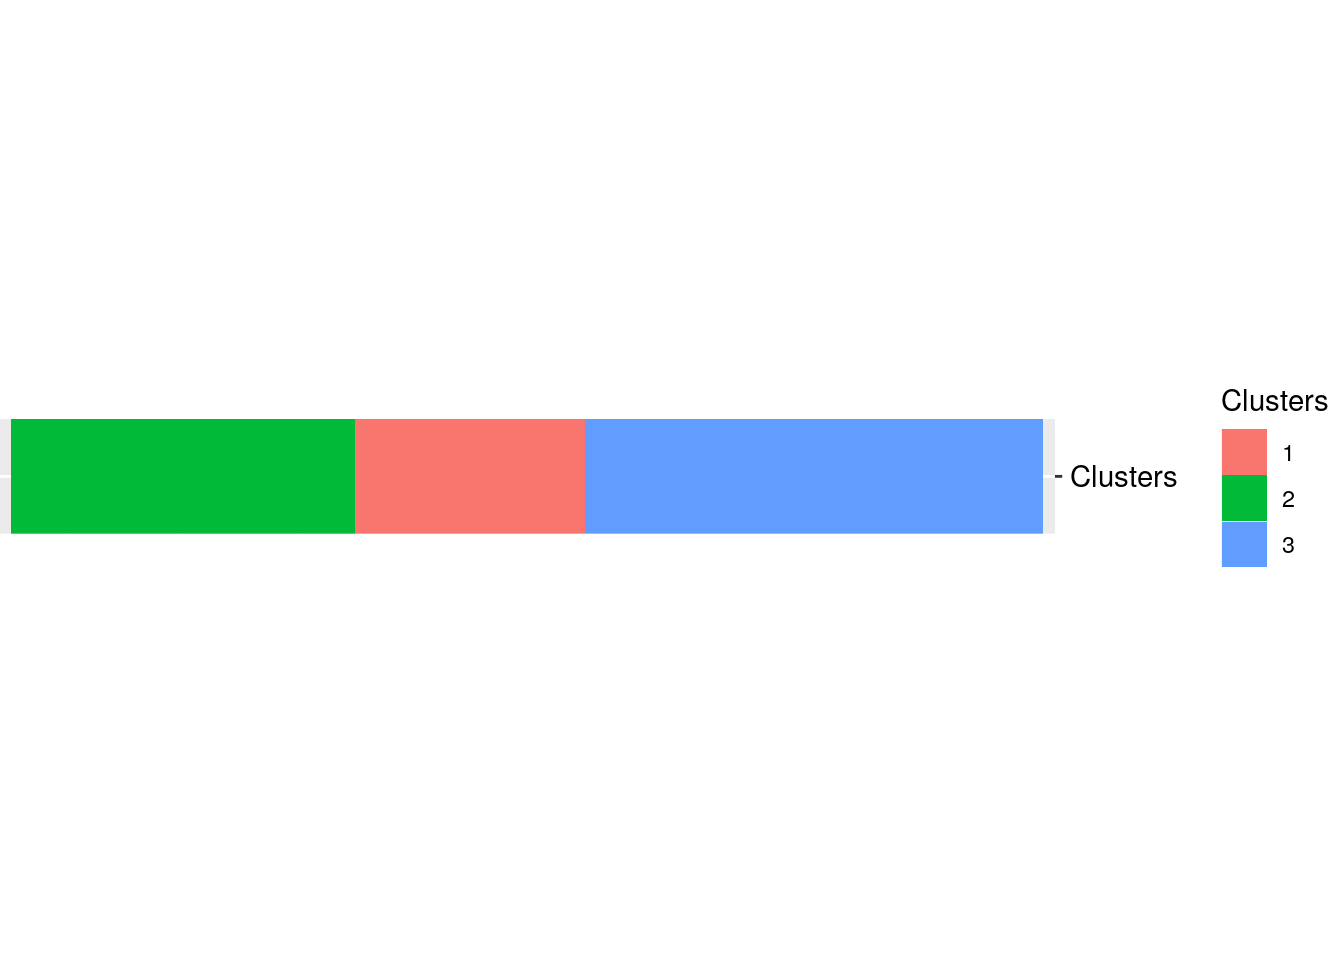
\includegraphics{21_microbiome_community_files/figure-latex/more_complex_heatmap3-1.pdf}

\begin{Shaded}
\begin{Highlighting}[]
\ControlFlowTok{if}\NormalTok{(}\SpecialCharTok{!}\FunctionTok{require}\NormalTok{(reshape2))\{}
    \FunctionTok{install.packages}\NormalTok{(}\StringTok{"reshape2"}\NormalTok{)}
    \FunctionTok{library}\NormalTok{(reshape2)}
\NormalTok{\}}
\CommentTok{\# Order data based on clusters and sample types}
\NormalTok{mat }\OtherTok{\textless{}{-}}\NormalTok{ mat[}\FunctionTok{unfactor}\NormalTok{(taxa\_clusters}\SpecialCharTok{$}\NormalTok{Feature), }\FunctionTok{unfactor}\NormalTok{(sample\_data}\SpecialCharTok{$}\NormalTok{sample)]}

\CommentTok{\# ggplot requires data in melted format}
\NormalTok{melted\_mat }\OtherTok{\textless{}{-}} \FunctionTok{melt}\NormalTok{(mat)}
\FunctionTok{colnames}\NormalTok{(melted\_mat) }\OtherTok{\textless{}{-}} \FunctionTok{c}\NormalTok{(}\StringTok{"Taxa"}\NormalTok{, }\StringTok{"Sample"}\NormalTok{, }\StringTok{"clr\_z"}\NormalTok{)}

\CommentTok{\# Determines the scaling of colorss}
\NormalTok{maxval }\OtherTok{\textless{}{-}} \FunctionTok{round}\NormalTok{(}\FunctionTok{max}\NormalTok{(}\FunctionTok{abs}\NormalTok{(melted\_mat}\SpecialCharTok{$}\NormalTok{clr\_z)))}
\NormalTok{limits }\OtherTok{\textless{}{-}} \FunctionTok{c}\NormalTok{(}\SpecialCharTok{{-}}\NormalTok{maxval, maxval)}
\NormalTok{breaks }\OtherTok{\textless{}{-}} \FunctionTok{seq}\NormalTok{(}\AttributeTok{from =} \FunctionTok{min}\NormalTok{(limits), }\AttributeTok{to =} \FunctionTok{max}\NormalTok{(limits), }\AttributeTok{by =} \FloatTok{0.5}\NormalTok{)}
\NormalTok{colours }\OtherTok{\textless{}{-}} \FunctionTok{c}\NormalTok{(}\StringTok{"darkblue"}\NormalTok{, }\StringTok{"blue"}\NormalTok{, }\StringTok{"white"}\NormalTok{, }\StringTok{"red"}\NormalTok{, }\StringTok{"darkred"}\NormalTok{)}

\NormalTok{heatmap }\OtherTok{\textless{}{-}} \FunctionTok{ggplot}\NormalTok{(melted\_mat) }\SpecialCharTok{+} 
  \FunctionTok{geom\_tile}\NormalTok{(}\FunctionTok{aes}\NormalTok{(}\AttributeTok{x =}\NormalTok{ Sample, }\AttributeTok{y =}\NormalTok{ Taxa, }\AttributeTok{fill =}\NormalTok{ clr\_z)) }\SpecialCharTok{+}
  \FunctionTok{theme}\NormalTok{(}
    \AttributeTok{axis.title.y=}\FunctionTok{element\_blank}\NormalTok{(),}
    \AttributeTok{axis.title.x=}\FunctionTok{element\_blank}\NormalTok{(),}
    \AttributeTok{axis.ticks.y=}\FunctionTok{element\_blank}\NormalTok{(),}
    \AttributeTok{axis.text.x =} \FunctionTok{element\_text}\NormalTok{(}\AttributeTok{angle =} \DecValTok{90}\NormalTok{, }\AttributeTok{vjust =} \FloatTok{0.5}\NormalTok{, }\AttributeTok{hjust=}\DecValTok{1}\NormalTok{),}
    
    \AttributeTok{plot.margin=}\FunctionTok{margin}\NormalTok{(}\DecValTok{0}\NormalTok{,}\DecValTok{0}\NormalTok{,}\DecValTok{0}\NormalTok{,}\DecValTok{0}\NormalTok{), }\CommentTok{\# removes margins}
    \AttributeTok{legend.key.height=} \FunctionTok{unit}\NormalTok{(}\DecValTok{1}\NormalTok{, }\StringTok{\textquotesingle{}cm\textquotesingle{}}\NormalTok{)}
\NormalTok{    ) }\SpecialCharTok{+}
  \FunctionTok{scale\_fill\_gradientn}\NormalTok{(}\AttributeTok{name =} \StringTok{"CLR + Z transform"}\NormalTok{, }
                       \AttributeTok{breaks =}\NormalTok{ breaks, }
                       \AttributeTok{limits =}\NormalTok{ limits, }
                       \AttributeTok{colours =}\NormalTok{ colours) }\SpecialCharTok{+} 
  \FunctionTok{scale\_y\_discrete}\NormalTok{(}\AttributeTok{position =} \StringTok{"right"}\NormalTok{)}

\NormalTok{heatmap}
\end{Highlighting}
\end{Shaded}

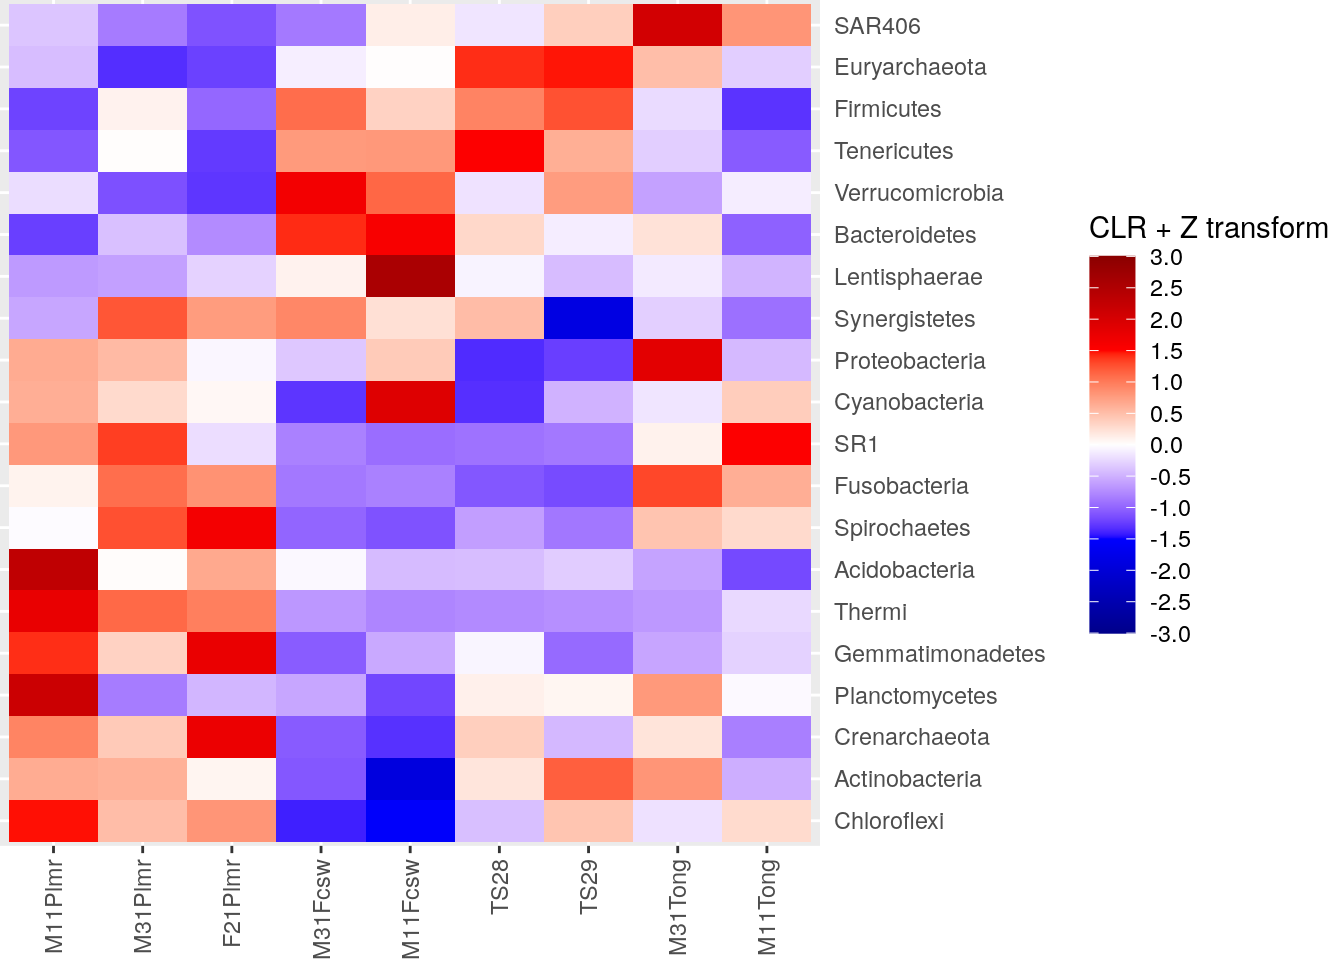
\includegraphics{21_microbiome_community_files/figure-latex/more_complex_heatmap4-1.pdf}

\begin{Shaded}
\begin{Highlighting}[]
\ControlFlowTok{if}\NormalTok{(}\SpecialCharTok{!}\FunctionTok{require}\NormalTok{(patchwork))\{}
    \FunctionTok{install.packages}\NormalTok{(}\StringTok{"patchwork"}\NormalTok{)}
    \FunctionTok{library}\NormalTok{(patchwork)}
\NormalTok{\}}

\CommentTok{\# Create layout}
\NormalTok{design }\OtherTok{\textless{}{-}} \FunctionTok{c}\NormalTok{(}
  \FunctionTok{area}\NormalTok{(}\DecValTok{3}\NormalTok{, }\DecValTok{1}\NormalTok{, }\DecValTok{4}\NormalTok{, }\DecValTok{1}\NormalTok{),}
  \FunctionTok{area}\NormalTok{(}\DecValTok{1}\NormalTok{, }\DecValTok{2}\NormalTok{, }\DecValTok{1}\NormalTok{, }\DecValTok{3}\NormalTok{),}
  \FunctionTok{area}\NormalTok{(}\DecValTok{2}\NormalTok{, }\DecValTok{2}\NormalTok{, }\DecValTok{2}\NormalTok{, }\DecValTok{3}\NormalTok{),}
  \FunctionTok{area}\NormalTok{(}\DecValTok{3}\NormalTok{, }\DecValTok{2}\NormalTok{, }\DecValTok{4}\NormalTok{, }\DecValTok{3}\NormalTok{)}
\NormalTok{)}

\FunctionTok{plot}\NormalTok{(design)}
\end{Highlighting}
\end{Shaded}

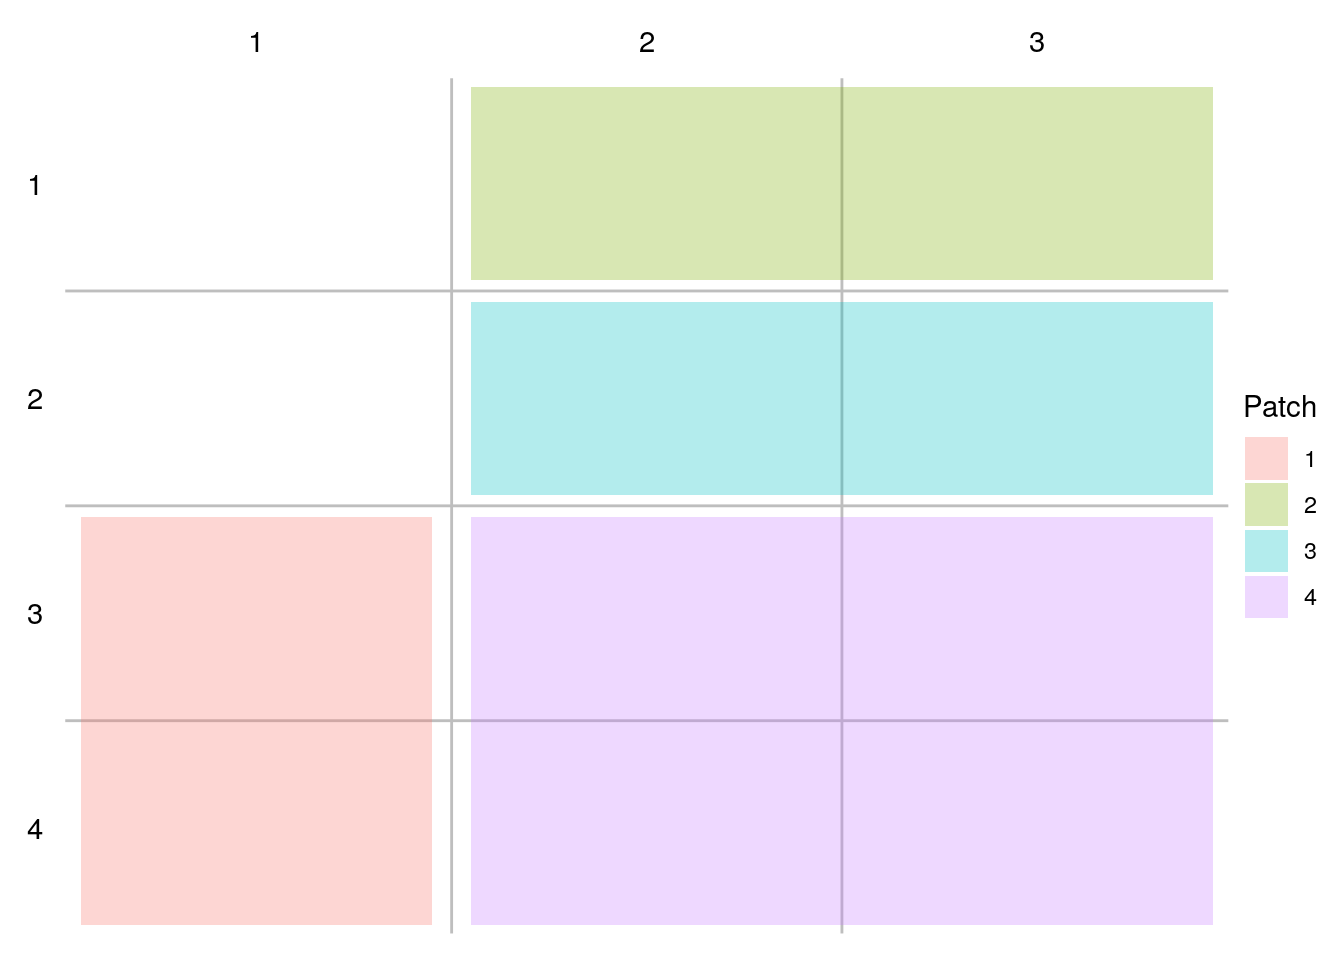
\includegraphics{21_microbiome_community_files/figure-latex/more_complex_heatmap5-1.pdf}

\begin{Shaded}
\begin{Highlighting}[]
\CommentTok{\# Combine plots}
\NormalTok{plot }\OtherTok{\textless{}{-}}\NormalTok{ row\_annotation }\SpecialCharTok{+}\NormalTok{ sample\_clusters\_annotation }\SpecialCharTok{+}\NormalTok{ sample\_types\_annotation }\SpecialCharTok{+}\NormalTok{ heatmap  }\SpecialCharTok{+}
    \FunctionTok{plot\_layout}\NormalTok{(}\AttributeTok{design =}\NormalTok{ design, }\AttributeTok{guides =} \StringTok{"collect"}\NormalTok{, }\CommentTok{\# Specify layout, collect legends}
                
                \CommentTok{\# Adjust widths and heights to align plots.}
                \CommentTok{\# When annotation plot is larger, it might not fit into its column/row.}
                \CommentTok{\# Then you need to make column/row larger.}
                
                \CommentTok{\# Relative widths and heights of each column and row:}
                \CommentTok{\# Currently, the width of the first column is 15 \% and the height of}
                \CommentTok{\# first two rows are 30 \% the size of others}
                
                \CommentTok{\# To get this work most of the times, you can adjust all sizes to be 1, i.e. equal, }
                \CommentTok{\# but then the gaps between plots are larger.}
                \AttributeTok{widths =} \FunctionTok{c}\NormalTok{(}\FloatTok{0.15}\NormalTok{, }\DecValTok{1}\NormalTok{, }\DecValTok{1}\NormalTok{),}
                \AttributeTok{heights =} \FunctionTok{c}\NormalTok{(}\FloatTok{0.3}\NormalTok{, }\FloatTok{0.3}\NormalTok{, }\DecValTok{1}\NormalTok{, }\DecValTok{1}\NormalTok{))}

\NormalTok{plot}
\end{Highlighting}
\end{Shaded}

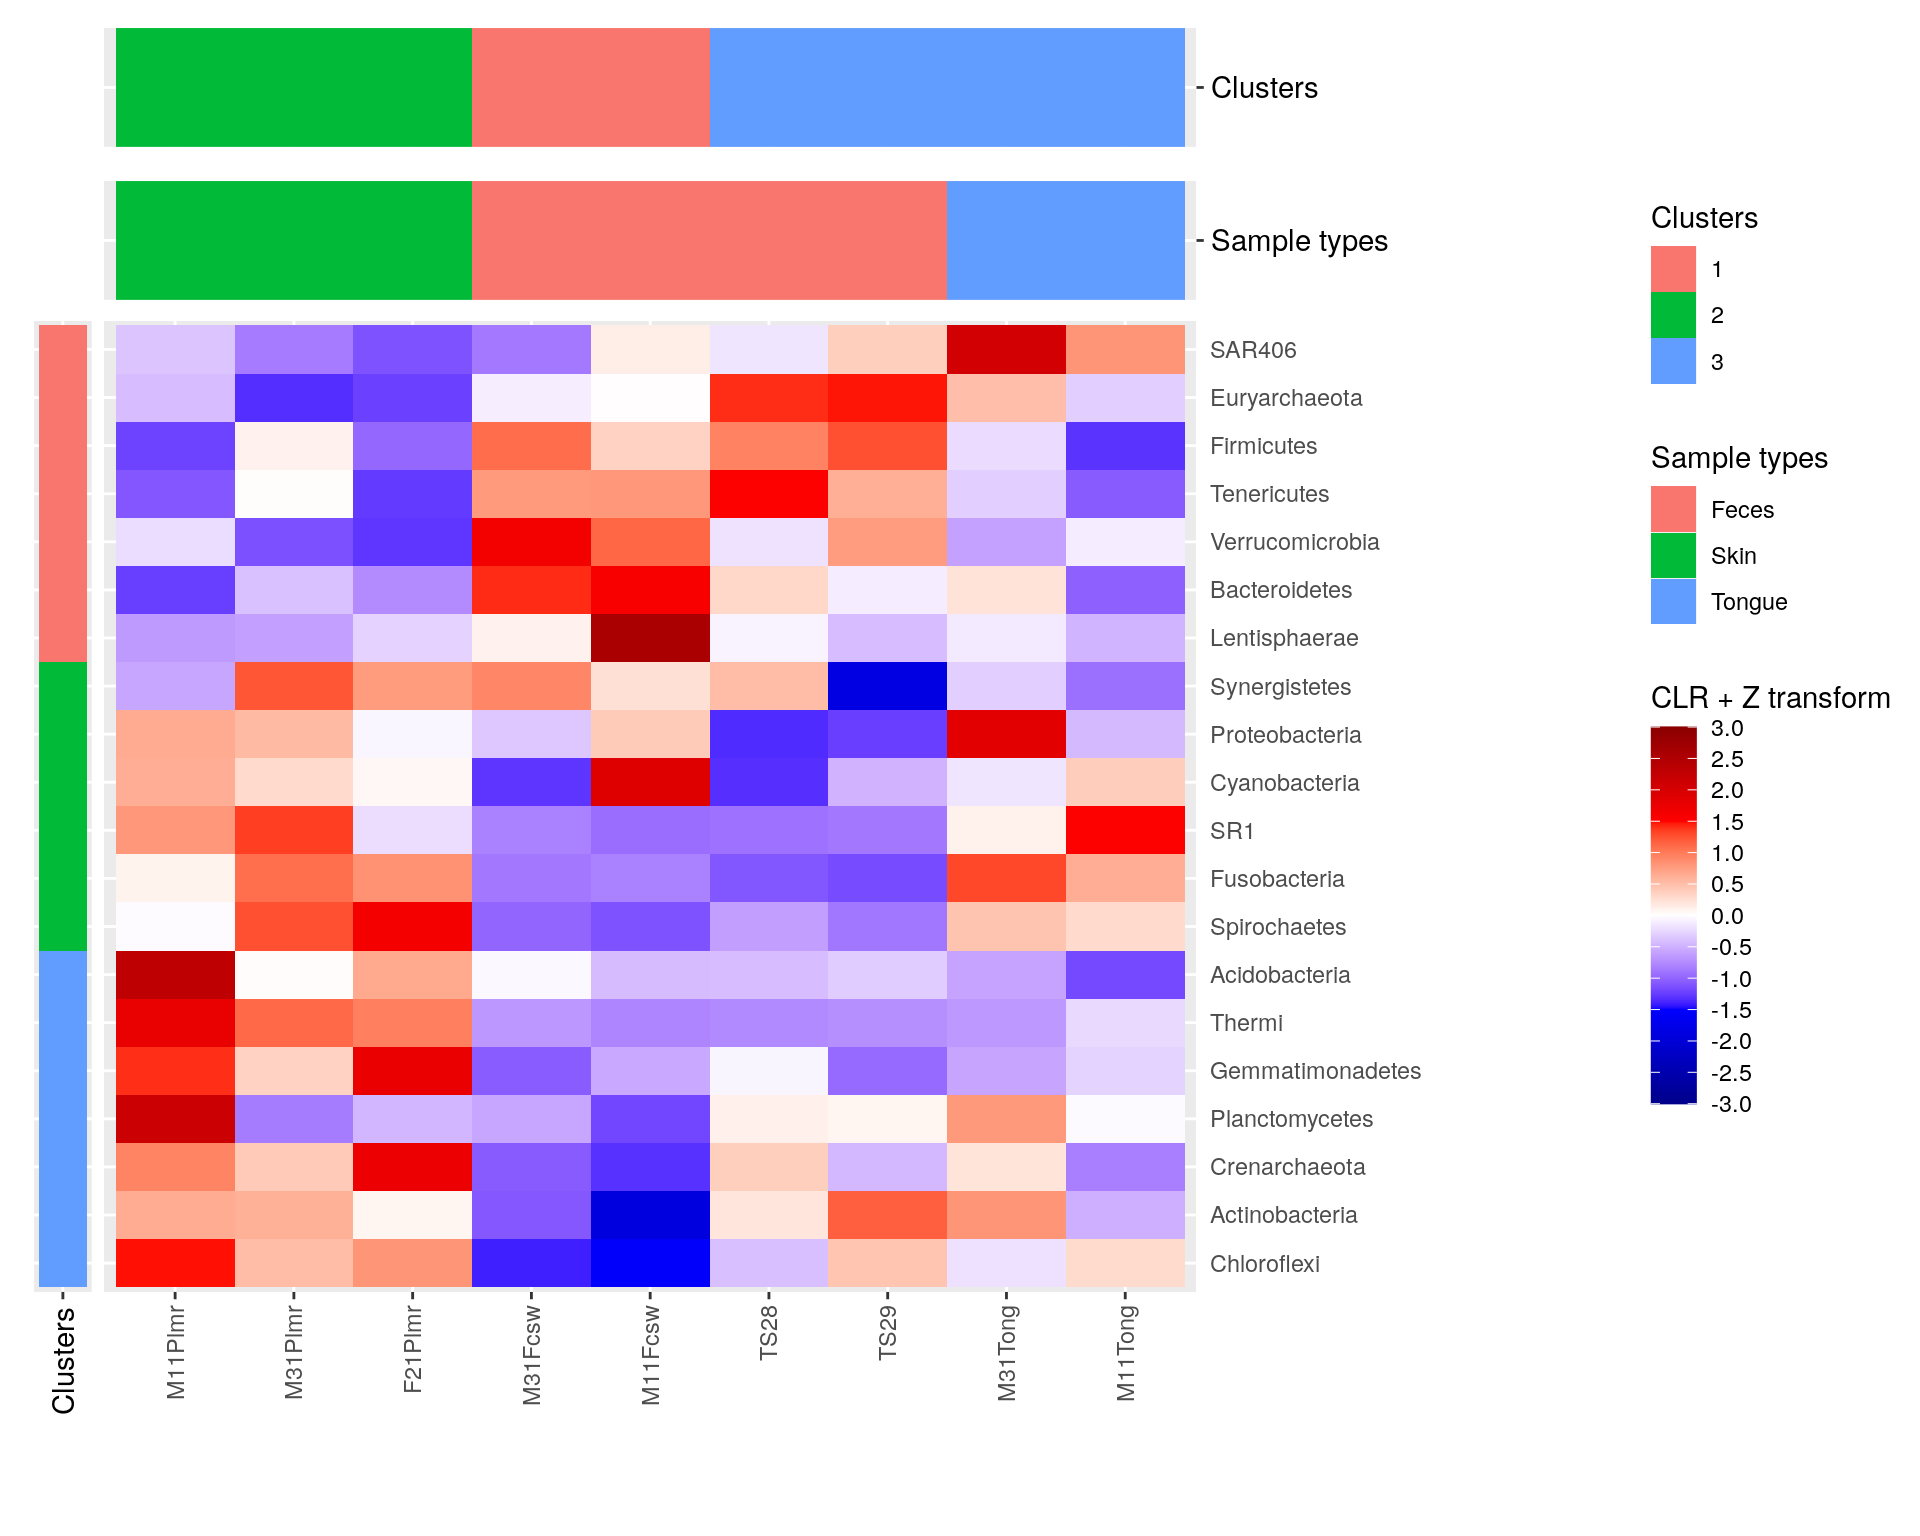
\includegraphics{21_microbiome_community_files/figure-latex/more_complex_heatmap6-1.pdf}

\begin{Shaded}
\begin{Highlighting}[]
\CommentTok{\# Create layout}
\NormalTok{design }\OtherTok{\textless{}{-}} \FunctionTok{c}\NormalTok{(}
  \FunctionTok{area}\NormalTok{(}\DecValTok{4}\NormalTok{, }\DecValTok{1}\NormalTok{, }\DecValTok{5}\NormalTok{, }\DecValTok{1}\NormalTok{),}
  \FunctionTok{area}\NormalTok{(}\DecValTok{4}\NormalTok{, }\DecValTok{2}\NormalTok{, }\DecValTok{5}\NormalTok{, }\DecValTok{2}\NormalTok{),}
  \FunctionTok{area}\NormalTok{(}\DecValTok{1}\NormalTok{, }\DecValTok{3}\NormalTok{, }\DecValTok{1}\NormalTok{, }\DecValTok{4}\NormalTok{),}
  \FunctionTok{area}\NormalTok{(}\DecValTok{2}\NormalTok{, }\DecValTok{3}\NormalTok{, }\DecValTok{2}\NormalTok{, }\DecValTok{4}\NormalTok{),}
  \FunctionTok{area}\NormalTok{(}\DecValTok{3}\NormalTok{, }\DecValTok{3}\NormalTok{, }\DecValTok{3}\NormalTok{, }\DecValTok{4}\NormalTok{),}
  \FunctionTok{area}\NormalTok{(}\DecValTok{4}\NormalTok{, }\DecValTok{3}\NormalTok{, }\DecValTok{5}\NormalTok{, }\DecValTok{4}\NormalTok{)}
\NormalTok{)}

\FunctionTok{plot}\NormalTok{(design)}
\end{Highlighting}
\end{Shaded}

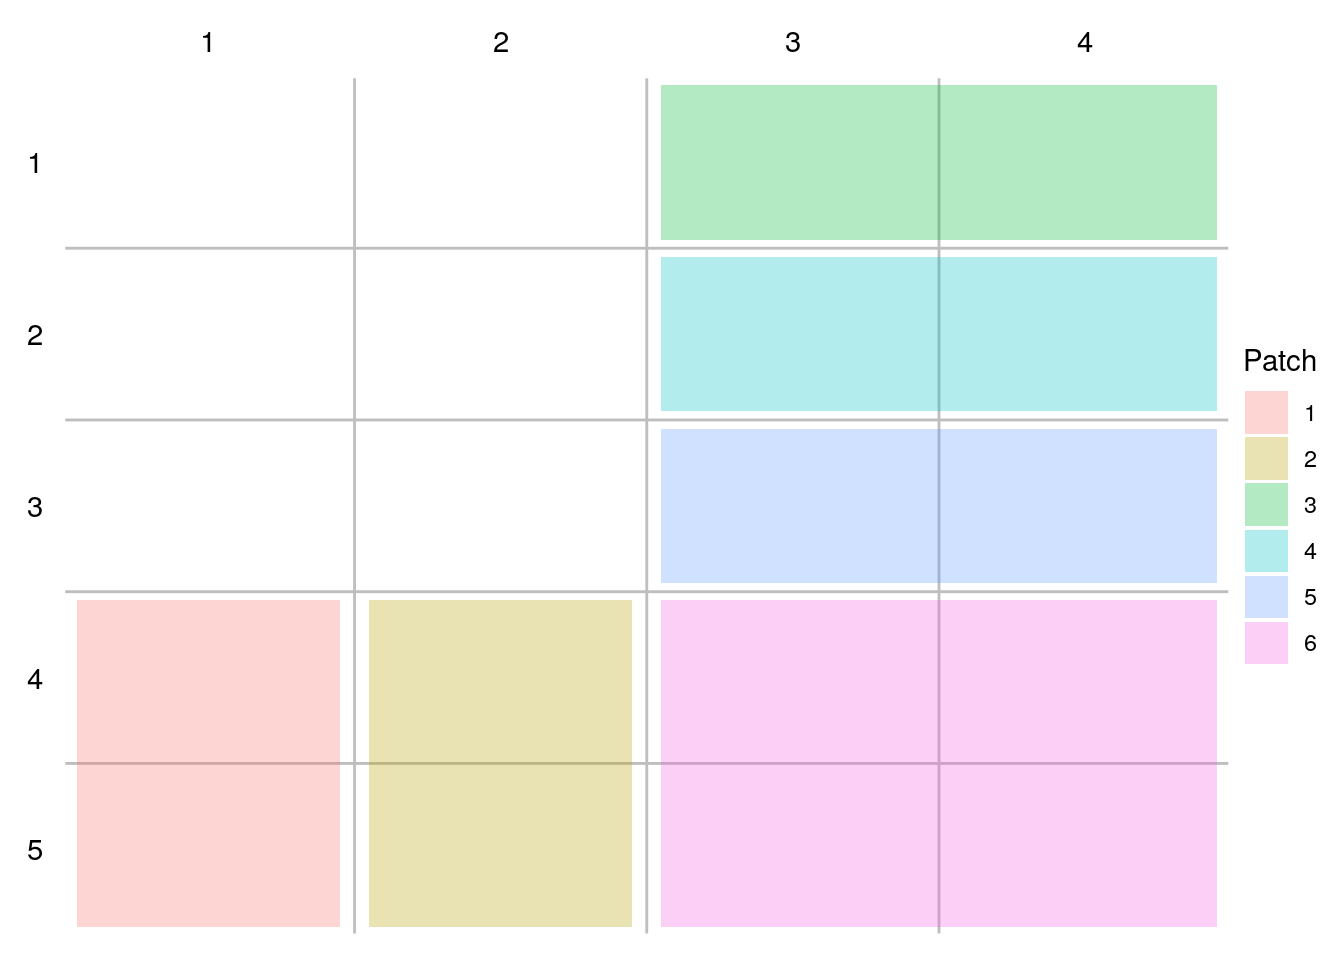
\includegraphics{21_microbiome_community_files/figure-latex/more_complex_heatmap7-1.pdf}

\begin{Shaded}
\begin{Highlighting}[]
\CommentTok{\# Combine plots}
\NormalTok{plot }\OtherTok{\textless{}{-}}\NormalTok{ taxa\_tree }\SpecialCharTok{+} 
\NormalTok{  row\_annotation }\SpecialCharTok{+}
\NormalTok{  sample\_tree }\SpecialCharTok{+} 
\NormalTok{  sample\_clusters\_annotation }\SpecialCharTok{+}
\NormalTok{  sample\_types\_annotation }\SpecialCharTok{+}
\NormalTok{  heatmap }\SpecialCharTok{+}
    \FunctionTok{plot\_layout}\NormalTok{(}\AttributeTok{design =}\NormalTok{ design, }\AttributeTok{guides =} \StringTok{"collect"}\NormalTok{, }\CommentTok{\# Specify layout, collect legends}
                \AttributeTok{widths =} \FunctionTok{c}\NormalTok{(}\FloatTok{0.2}\NormalTok{, }\FloatTok{0.15}\NormalTok{, }\DecValTok{1}\NormalTok{, }\DecValTok{1}\NormalTok{, }\DecValTok{1}\NormalTok{),}
                \AttributeTok{heights =} \FunctionTok{c}\NormalTok{(}\FloatTok{0.1}\NormalTok{, }\FloatTok{0.15}\NormalTok{, }\FloatTok{0.15}\NormalTok{, }\FloatTok{0.25}\NormalTok{, }\DecValTok{1}\NormalTok{, }\DecValTok{1}\NormalTok{))}

\NormalTok{plot}
\end{Highlighting}
\end{Shaded}

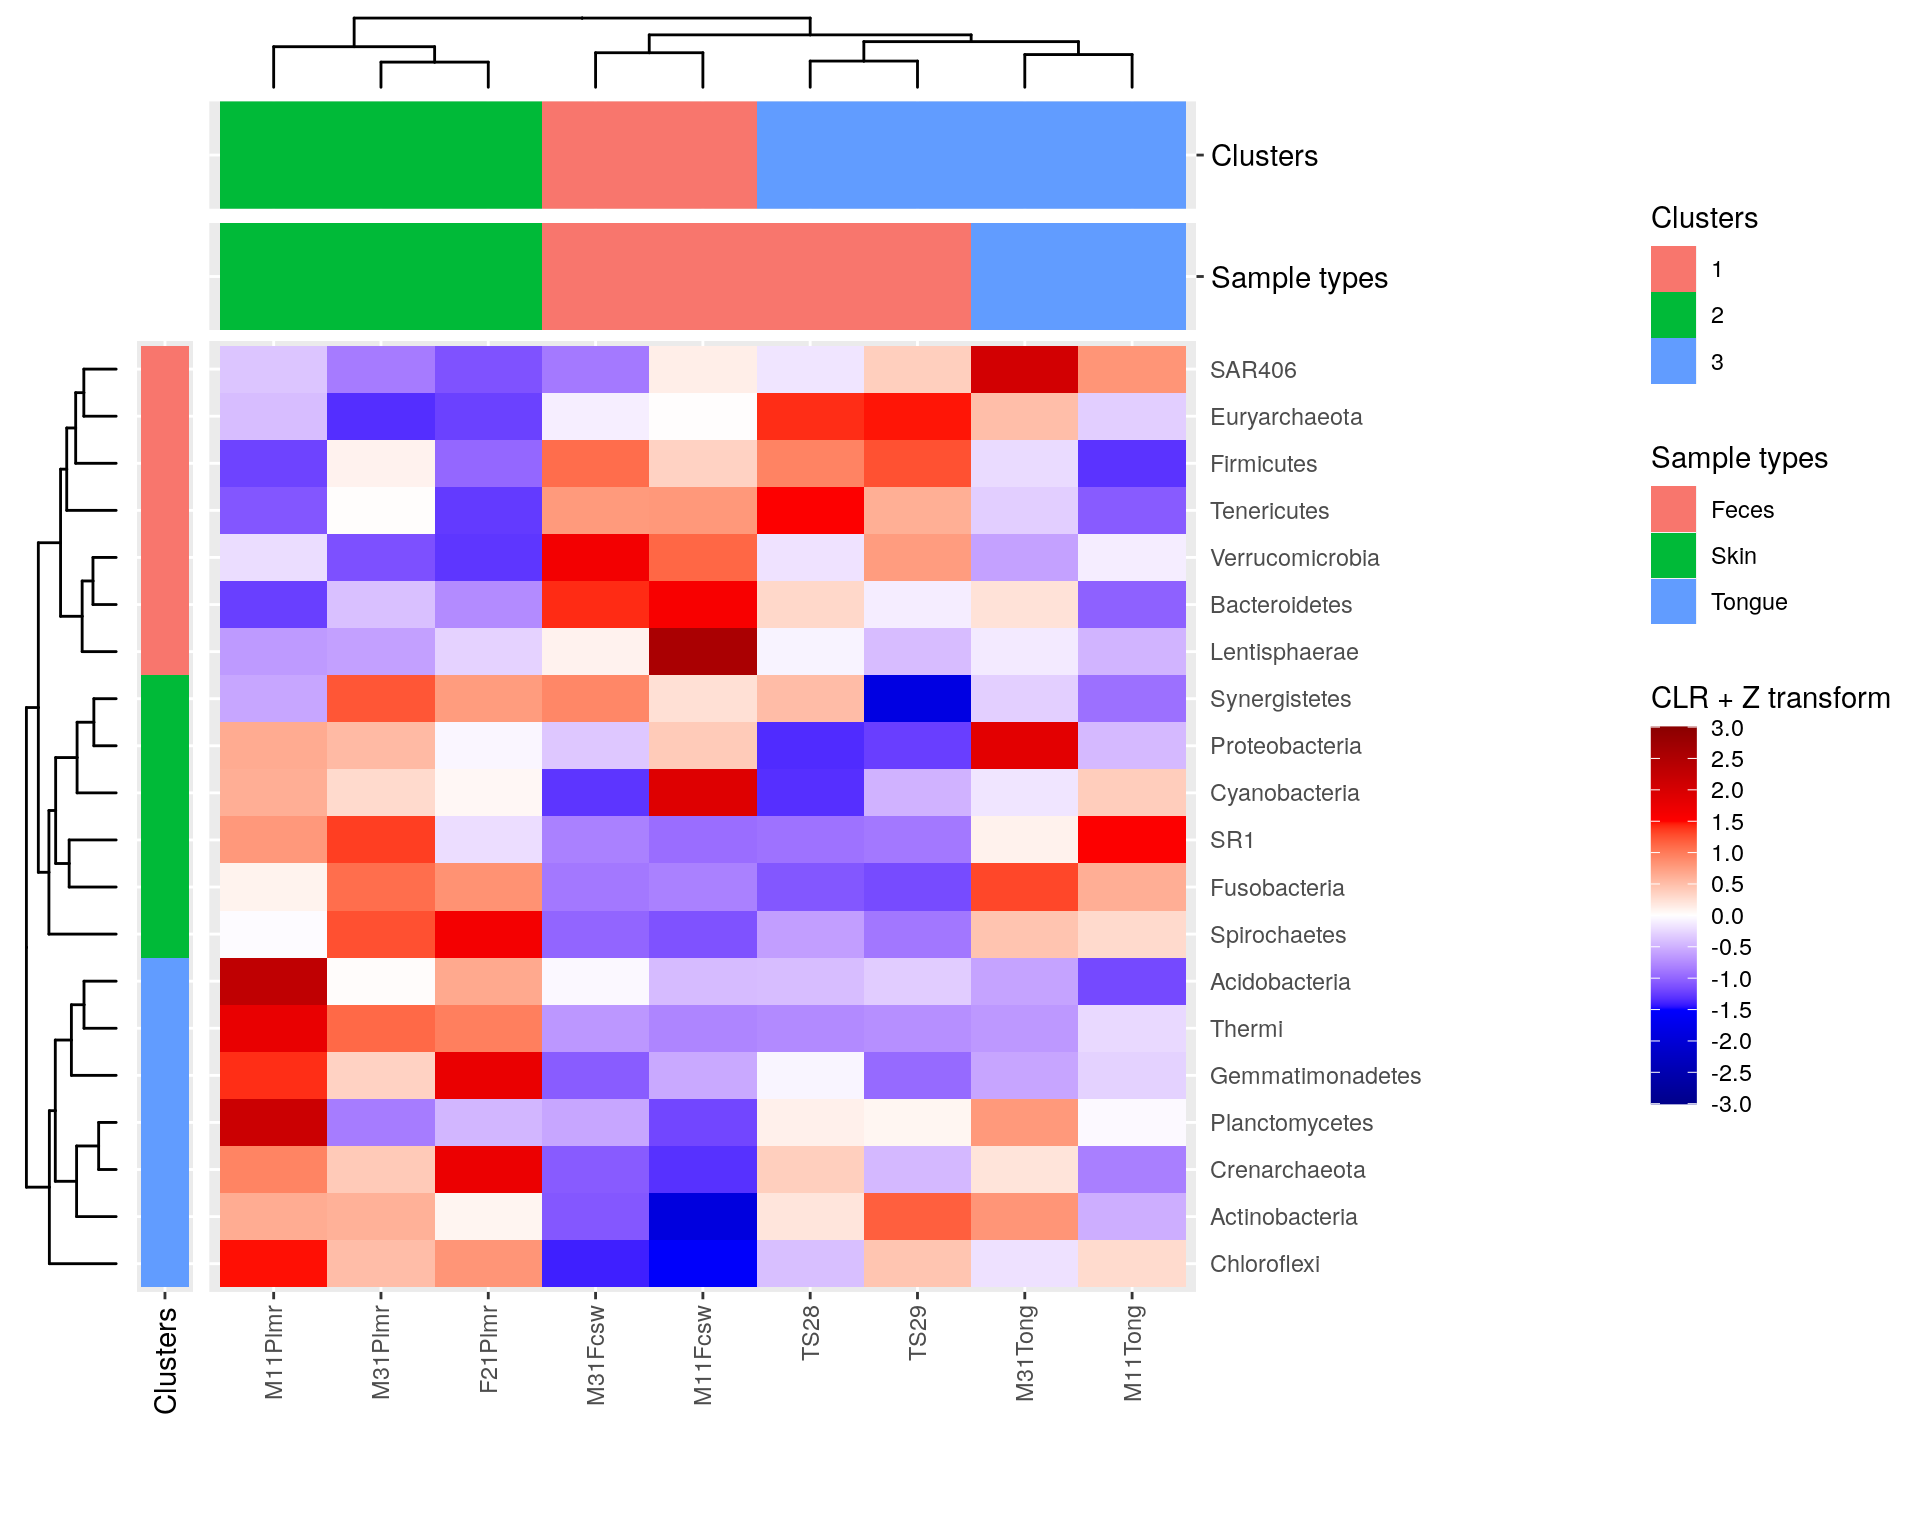
\includegraphics{21_microbiome_community_files/figure-latex/more_complex_heatmap8-1.pdf}

\hypertarget{community-typing}{%
\chapter{Community typing}\label{community-typing}}

\hypertarget{dirichlet-multinomial-mixtures-dmm}{%
\section{Dirichlet Multinomial Mixtures (DMM)}\label{dirichlet-multinomial-mixtures-dmm}}

This section focus on DMM analysis.

One technique that allows to search for groups of samples that are
similar to each other is the \href{https://journals.plos.org/plosone/article?id=10.1371/journal.pone.0030126}{Dirichlet-Multinomial Mixture
Model}. In
DMM, we first determine the number of clusters (k) that best fit the
data (model evidence) using Laplace approximation. After fitting the
model with k clusters, we obtain for each sample k probabilities that
reflect the probability that a sample belongs to the given cluster.

Let's cluster the data with DMM clustering.

\begin{Shaded}
\begin{Highlighting}[]
\CommentTok{\# Runs model and calculates the most likely number of clusters from 1 to 7.}
\CommentTok{\# Since this is a large dataset it takes long computational time.}
\CommentTok{\# For this reason we use only a subset of the data; agglomerated by Phylum as a rank.}
\NormalTok{tse }\OtherTok{\textless{}{-}}\NormalTok{ GlobalPatterns}
\NormalTok{tse }\OtherTok{\textless{}{-}} \FunctionTok{agglomerateByRank}\NormalTok{(tse, }\AttributeTok{rank =} \StringTok{"Phylum"}\NormalTok{, }\AttributeTok{agglomerateTree=}\ConstantTok{TRUE}\NormalTok{)}
\end{Highlighting}
\end{Shaded}

\begin{Shaded}
\begin{Highlighting}[]
\NormalTok{tse\_dmn }\OtherTok{\textless{}{-}}\NormalTok{ mia}\SpecialCharTok{::}\FunctionTok{runDMN}\NormalTok{(tse, }\AttributeTok{name =} \StringTok{"DMN"}\NormalTok{, }\AttributeTok{k =} \DecValTok{1}\SpecialCharTok{:}\DecValTok{7}\NormalTok{)}
\end{Highlighting}
\end{Shaded}

\begin{Shaded}
\begin{Highlighting}[]
\CommentTok{\# It is stored in metadata}
\NormalTok{tse\_dmn}
\end{Highlighting}
\end{Shaded}

\begin{verbatim}
## class: TreeSummarizedExperiment 
## dim: 67 26 
## metadata(2): agglomerated_by_rank DMN
## assays(1): counts
## rownames(67): Phylum:Crenarchaeota Phylum:Euryarchaeota ...
##   Phylum:Synergistetes Phylum:SR1
## rowData names(7): Kingdom Phylum ... Genus Species
## colnames(26): CL3 CC1 ... Even2 Even3
## colData names(7): X.SampleID Primer ... SampleType Description
## reducedDimNames(0):
## mainExpName: NULL
## altExpNames(0):
## rowLinks: a LinkDataFrame (67 rows)
## rowTree: 1 phylo tree(s) (66 leaves)
## colLinks: NULL
## colTree: NULL
\end{verbatim}

Return information on metadata that the object contains.

\begin{Shaded}
\begin{Highlighting}[]
\FunctionTok{names}\NormalTok{(}\FunctionTok{metadata}\NormalTok{(tse\_dmn))}
\end{Highlighting}
\end{Shaded}

\begin{verbatim}
## [1] "agglomerated_by_rank" "DMN"
\end{verbatim}

This returns a list of DMN objects for a closer investigation.

\begin{Shaded}
\begin{Highlighting}[]
\FunctionTok{getDMN}\NormalTok{(tse\_dmn)}
\end{Highlighting}
\end{Shaded}

\begin{verbatim}
## [[1]]
## class: DMN 
## k: 1 
## samples x taxa: 26 x 67 
## Laplace: 7715 BIC: 7802 AIC: 7760 
## 
## [[2]]
## class: DMN 
## k: 2 
## samples x taxa: 26 x 67 
## Laplace: 7673 BIC: 7927 AIC: 7842 
## 
## [[3]]
## class: DMN 
## k: 3 
## samples x taxa: 26 x 67 
## Laplace: 7690 BIC: 8076 AIC: 7948 
## 
## [[4]]
## class: DMN 
## k: 4 
## samples x taxa: 26 x 67 
## Laplace: 7792 BIC: 8357 AIC: 8187 
## 
## [[5]]
## class: DMN 
## k: 5 
## samples x taxa: 26 x 67 
## Laplace: 7860 BIC: 8604 AIC: 8391 
## 
## [[6]]
## class: DMN 
## k: 6 
## samples x taxa: 26 x 67 
## Laplace: 7943 BIC: 8822 AIC: 8566 
## 
## [[7]]
## class: DMN 
## k: 7 
## samples x taxa: 26 x 67 
## Laplace: 8055 BIC: 9123 AIC: 8824
\end{verbatim}

Show Laplace approximation (model evidence) for each model of the k models.

\begin{Shaded}
\begin{Highlighting}[]
\FunctionTok{library}\NormalTok{(miaViz)}
\FunctionTok{plotDMNFit}\NormalTok{(tse\_dmn, }\AttributeTok{type =} \StringTok{"laplace"}\NormalTok{)}
\end{Highlighting}
\end{Shaded}

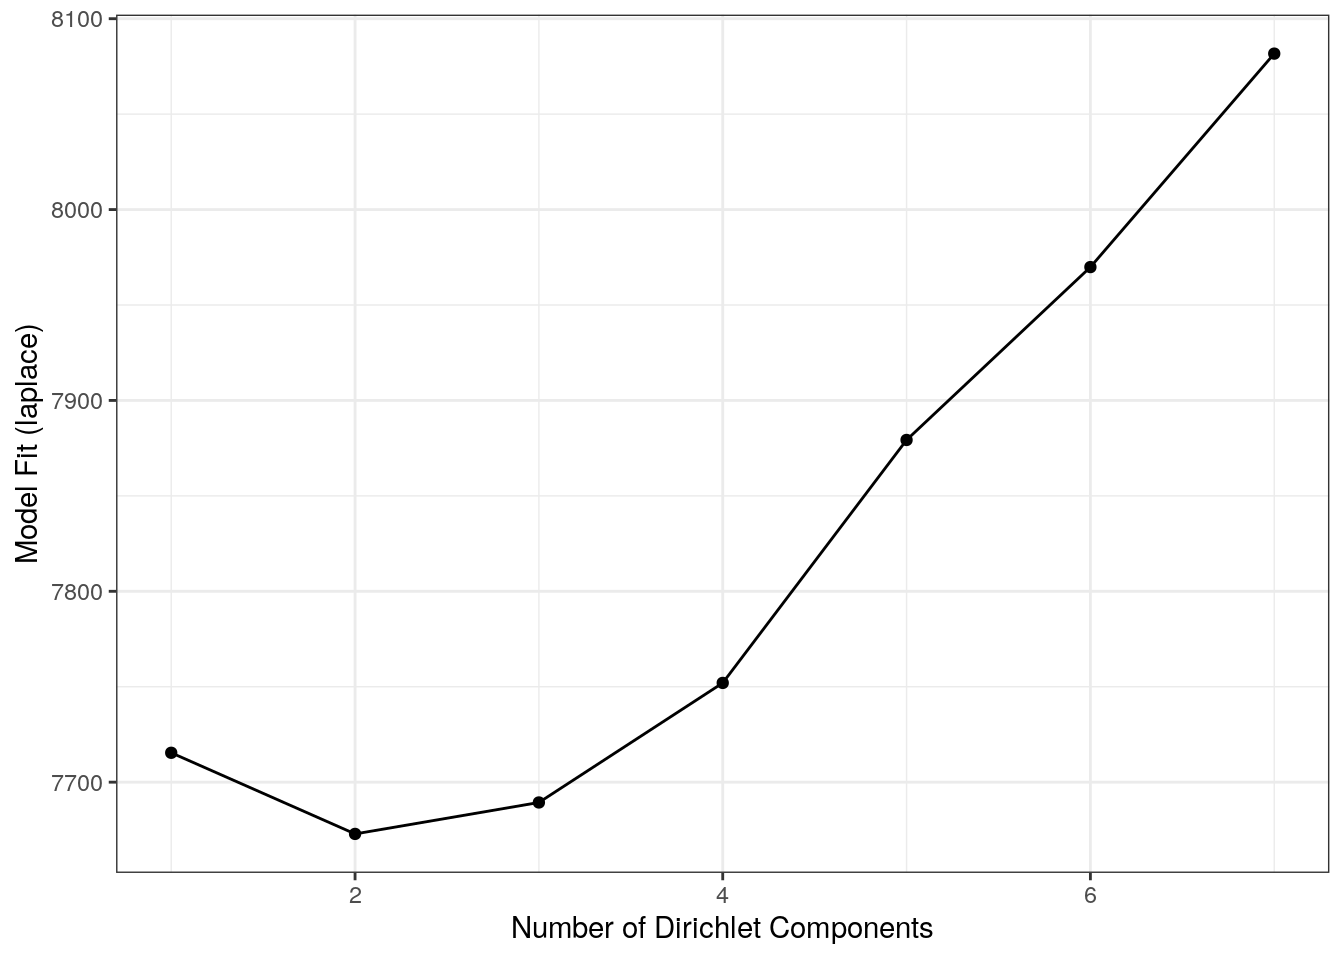
\includegraphics{21_microbiome_community_files/figure-latex/unnamed-chunk-5-1.pdf}

Return the model that has the best fit.

\begin{Shaded}
\begin{Highlighting}[]
\FunctionTok{getBestDMNFit}\NormalTok{(tse\_dmn, }\AttributeTok{type =} \StringTok{"laplace"}\NormalTok{)}
\end{Highlighting}
\end{Shaded}

\begin{verbatim}
## class: DMN 
## k: 2 
## samples x taxa: 26 x 67 
## Laplace: 7673 BIC: 7927 AIC: 7842
\end{verbatim}

\hypertarget{pcoa-for-asv-level-data-with-bray-curtis-with-dmm-clusters-shown-with-colors}{%
\subsection{PCoA for ASV-level data with Bray-Curtis; with DMM clusters shown with colors}\label{pcoa-for-asv-level-data-with-bray-curtis-with-dmm-clusters-shown-with-colors}}

Group samples and return DMNGroup object that contains a summary.
Patient status is used for grouping.

\begin{Shaded}
\begin{Highlighting}[]
\NormalTok{dmn\_group }\OtherTok{\textless{}{-}} \FunctionTok{calculateDMNgroup}\NormalTok{(tse\_dmn, }\AttributeTok{variable =} \StringTok{"SampleType"}\NormalTok{,  }\AttributeTok{exprs\_values =} \StringTok{"counts"}\NormalTok{,}
                               \AttributeTok{k =} \DecValTok{2}\NormalTok{, }\AttributeTok{seed=}\NormalTok{.Machine}\SpecialCharTok{$}\NormalTok{integer.max)}

\NormalTok{dmn\_group}
\end{Highlighting}
\end{Shaded}

\begin{verbatim}
## class: DMNGroup 
## summary:
##                    k samples taxa    NLE  LogDet Laplace    BIC  AIC
## Feces              2       4   67 1078.3 -106.19   901.1 1171.9 1213
## Freshwater         2       2   67  889.6  -97.28   716.9  936.4 1025
## Freshwater (creek) 2       3   67 1600.3  860.08  1906.3 1674.5 1735
## Mock               2       3   67 1008.4  -55.37   856.6 1082.5 1143
## Ocean              2       3   67 1096.7  -56.21   944.6 1170.9 1232
## Sediment (estuary) 2       3   67 1195.5   18.63  1080.8 1269.7 1331
## Skin               2       3   67  992.6  -84.81   826.2 1066.8 1128
## Soil               2       3   67 1380.3   11.21  1261.8 1454.5 1515
## Tongue             2       2   67  783.0 -107.74   605.1  829.8  918
\end{verbatim}

Mixture weights (rough measure of the cluster size).

\begin{Shaded}
\begin{Highlighting}[]
\NormalTok{DirichletMultinomial}\SpecialCharTok{::}\FunctionTok{mixturewt}\NormalTok{(}\FunctionTok{getBestDMNFit}\NormalTok{(tse\_dmn))}
\end{Highlighting}
\end{Shaded}

\begin{verbatim}
##       pi theta
## 1 0.5385 20.58
## 2 0.4615 15.28
\end{verbatim}

Samples-cluster assignment probabilities / how probable it is that sample belongs
to each cluster

\begin{Shaded}
\begin{Highlighting}[]
\FunctionTok{head}\NormalTok{(DirichletMultinomial}\SpecialCharTok{::}\FunctionTok{mixture}\NormalTok{(}\FunctionTok{getBestDMNFit}\NormalTok{(tse\_dmn)))}
\end{Highlighting}
\end{Shaded}

\begin{verbatim}
##              [,1]      [,2]
## CL3     1.000e+00 5.024e-17
## CC1     1.000e+00 3.871e-22
## SV1     1.000e+00 1.946e-12
## M31Fcsw 7.904e-26 1.000e+00
## M11Fcsw 1.135e-16 1.000e+00
## M31Plmr 1.126e-13 1.000e+00
\end{verbatim}

Contribution of each taxa to each component

\begin{Shaded}
\begin{Highlighting}[]
\FunctionTok{head}\NormalTok{(DirichletMultinomial}\SpecialCharTok{::}\FunctionTok{fitted}\NormalTok{(}\FunctionTok{getBestDMNFit}\NormalTok{(tse\_dmn)))}
\end{Highlighting}
\end{Shaded}

\begin{verbatim}
##                          [,1]      [,2]
## Phylum:Crenarchaeota  0.30385 0.1354653
## Phylum:Euryarchaeota  0.23116 0.1468628
## Phylum:Actinobacteria 1.21385 1.0600329
## Phylum:Spirochaetes   0.21394 0.1318413
## Phylum:MVP-15         0.02982 0.0007654
## Phylum:Proteobacteria 6.84333 1.8153087
\end{verbatim}

Get the assignment probabilities

\begin{Shaded}
\begin{Highlighting}[]
\NormalTok{prob }\OtherTok{\textless{}{-}}\NormalTok{ DirichletMultinomial}\SpecialCharTok{::}\FunctionTok{mixture}\NormalTok{(}\FunctionTok{getBestDMNFit}\NormalTok{(tse\_dmn))}
\CommentTok{\# Add column names}
\FunctionTok{colnames}\NormalTok{(prob) }\OtherTok{\textless{}{-}} \FunctionTok{c}\NormalTok{(}\StringTok{"comp1"}\NormalTok{, }\StringTok{"comp2"}\NormalTok{)}

\CommentTok{\# For each row, finds column that has the highest value. Then extract the column }
\CommentTok{\# names of highest values.}
\NormalTok{vec }\OtherTok{\textless{}{-}} \FunctionTok{colnames}\NormalTok{(prob)[}\FunctionTok{max.col}\NormalTok{(prob,}\AttributeTok{ties.method =} \StringTok{"first"}\NormalTok{)]}
\end{Highlighting}
\end{Shaded}

Computing the euclidean PCoA and storing it as a data frame

\begin{Shaded}
\begin{Highlighting}[]
\CommentTok{\# Does clr transformation. Pseudocount is added, because data contains zeros.}
\NormalTok{tse }\OtherTok{\textless{}{-}} \FunctionTok{transformCounts}\NormalTok{(tse, }\AttributeTok{method =} \StringTok{"clr"}\NormalTok{, }\AttributeTok{pseudocount =} \DecValTok{1}\NormalTok{)}

\CommentTok{\# Gets clr table}
\NormalTok{clr\_assay }\OtherTok{\textless{}{-}} \FunctionTok{assays}\NormalTok{(tse)}\SpecialCharTok{$}\NormalTok{clr}

\CommentTok{\# Transposes it to get taxa to columns}
\NormalTok{clr\_assay }\OtherTok{\textless{}{-}} \FunctionTok{t}\NormalTok{(clr\_assay)}

\CommentTok{\# Calculates Euclidean distances between samples. Because taxa is in columns,}
\CommentTok{\# it is used to compare different samples.}
\NormalTok{euclidean\_dist }\OtherTok{\textless{}{-}}\NormalTok{ vegan}\SpecialCharTok{::}\FunctionTok{vegdist}\NormalTok{(clr\_assay, }\AttributeTok{method =} \StringTok{"euclidean"}\NormalTok{)}

\CommentTok{\# Does principal coordinate analysis}
\NormalTok{euclidean\_pcoa }\OtherTok{\textless{}{-}}\NormalTok{ ecodist}\SpecialCharTok{::}\FunctionTok{pco}\NormalTok{(euclidean\_dist)}

\CommentTok{\# Creates a data frame from principal coordinates}
\NormalTok{euclidean\_pcoa\_df }\OtherTok{\textless{}{-}} \FunctionTok{data.frame}\NormalTok{(}\AttributeTok{pcoa1 =}\NormalTok{ euclidean\_pcoa}\SpecialCharTok{$}\NormalTok{vectors[,}\DecValTok{1}\NormalTok{], }
                                \AttributeTok{pcoa2 =}\NormalTok{ euclidean\_pcoa}\SpecialCharTok{$}\NormalTok{vectors[,}\DecValTok{2}\NormalTok{])}
\end{Highlighting}
\end{Shaded}

\begin{Shaded}
\begin{Highlighting}[]
\CommentTok{\# Creates a data frame that contains principal coordinates and DMM information}
\NormalTok{euclidean\_dmm\_pcoa\_df }\OtherTok{\textless{}{-}} \FunctionTok{cbind}\NormalTok{(euclidean\_pcoa\_df,}
                               \AttributeTok{dmm\_component =}\NormalTok{ vec)}
\CommentTok{\# Creates a plot}
\NormalTok{euclidean\_dmm\_plot }\OtherTok{\textless{}{-}} \FunctionTok{ggplot}\NormalTok{(}\AttributeTok{data =}\NormalTok{ euclidean\_dmm\_pcoa\_df, }
                             \FunctionTok{aes}\NormalTok{(}\AttributeTok{x=}\NormalTok{pcoa1, }\AttributeTok{y=}\NormalTok{pcoa2,}
                                 \AttributeTok{color =}\NormalTok{ dmm\_component)) }\SpecialCharTok{+}
  \FunctionTok{geom\_point}\NormalTok{() }\SpecialCharTok{+}
  \FunctionTok{labs}\NormalTok{(}\AttributeTok{x =} \StringTok{"Coordinate 1"}\NormalTok{,}
       \AttributeTok{y =} \StringTok{"Coordinate 2"}\NormalTok{,}
       \AttributeTok{title =} \StringTok{"PCoA with Aitchison distances"}\NormalTok{) }\SpecialCharTok{+}  
  \FunctionTok{theme}\NormalTok{(}\AttributeTok{title =} \FunctionTok{element\_text}\NormalTok{(}\AttributeTok{size =} \DecValTok{12}\NormalTok{)) }\CommentTok{\# makes titles smaller}

\NormalTok{euclidean\_dmm\_plot}
\end{Highlighting}
\end{Shaded}

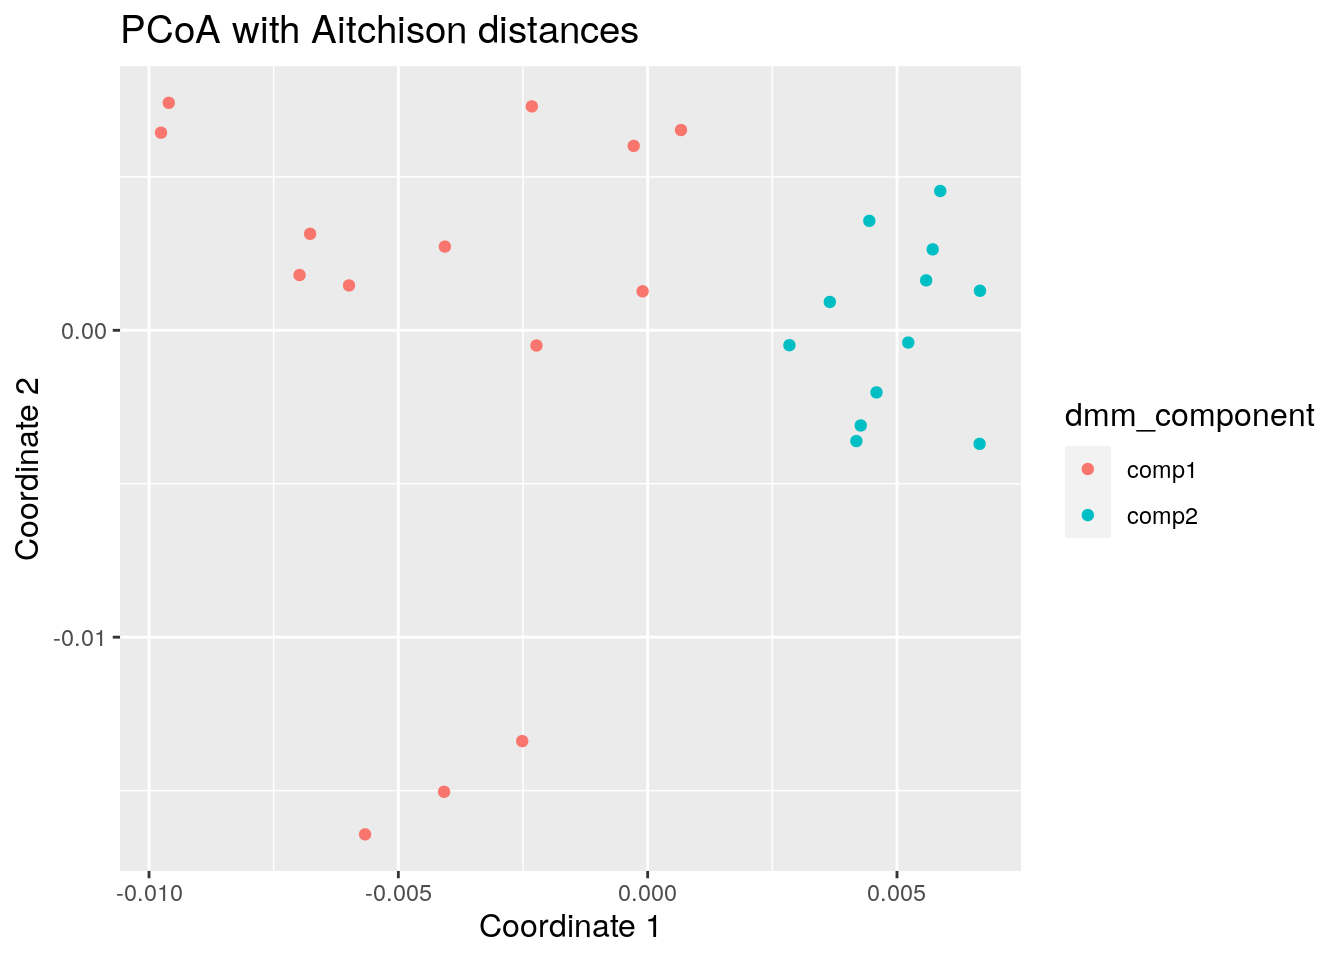
\includegraphics{21_microbiome_community_files/figure-latex/unnamed-chunk-13-1.pdf}

\hypertarget{community-detection}{%
\section{Community Detection}\label{community-detection}}

Another approach for discovering communities within the samples of the
data, is to run community detection algorithms after building a
graph. The following demonstration builds a graph based on the k
nearest-neighbors and performs the community detection on the fly.

\emph{\texttt{bluster}} \citep{R-bluster} package offers several clustering methods,
among which graph-based are present, enabling the community detection
task.

Installing package:

\begin{Shaded}
\begin{Highlighting}[]
\ControlFlowTok{if}\NormalTok{(}\SpecialCharTok{!}\FunctionTok{require}\NormalTok{(bluster))\{}
\NormalTok{  BiocManager}\SpecialCharTok{::}\FunctionTok{install}\NormalTok{(}\StringTok{"bluster"}\NormalTok{)}
\NormalTok{\}}
\end{Highlighting}
\end{Shaded}

The algorithm used is ``short random walks'' \citep{Pons2006}. Graph is
constructed using different k values (the number of nearest neighbors
to consider during graph construction) using the robust centered log
ratio (rclr) assay data. Then plotting the communities using UMAP
\citep{McInnes2018} ordination as a visual exploration aid. In the
following demonstration we use the \texttt{enterotype} dataset from the
\citep{R-mia} package.

\begin{Shaded}
\begin{Highlighting}[]
\FunctionTok{library}\NormalTok{(bluster)}
\FunctionTok{library}\NormalTok{(patchwork) }\CommentTok{\# For arranging several plots as a grid}
\FunctionTok{library}\NormalTok{(scater)}

\FunctionTok{data}\NormalTok{(}\StringTok{"enterotype"}\NormalTok{, }\AttributeTok{package=}\StringTok{"mia"}\NormalTok{)}
\NormalTok{tse }\OtherTok{\textless{}{-}}\NormalTok{ enterotype}
\NormalTok{tse }\OtherTok{\textless{}{-}} \FunctionTok{transformCounts}\NormalTok{(tse, }\AttributeTok{method =} \StringTok{"rclr"}\NormalTok{)}

\CommentTok{\# Performing and storing UMAP}
\NormalTok{tse }\OtherTok{\textless{}{-}} \FunctionTok{runUMAP}\NormalTok{(tse, }\AttributeTok{name=}\StringTok{"UMAP"}\NormalTok{, }\AttributeTok{exprs\_values=}\StringTok{"rclr"}\NormalTok{)}

\NormalTok{k }\OtherTok{\textless{}{-}} \FunctionTok{c}\NormalTok{(}\DecValTok{2}\NormalTok{,}\DecValTok{3}\NormalTok{,}\DecValTok{5}\NormalTok{,}\DecValTok{10}\NormalTok{)}
\NormalTok{ClustAndPlot }\OtherTok{\textless{}{-}} \ControlFlowTok{function}\NormalTok{(x) \{}
  \CommentTok{\# Creating the graph and running the short random walks algorithm  }
\NormalTok{  graph\_clusters }\OtherTok{\textless{}{-}} \FunctionTok{clusterRows}\NormalTok{(}\FunctionTok{t}\NormalTok{(}\FunctionTok{assays}\NormalTok{(tse)}\SpecialCharTok{$}\NormalTok{rclr), }\FunctionTok{NNGraphParam}\NormalTok{(}\AttributeTok{k=}\NormalTok{x))}
  
  \CommentTok{\# Results of the clustering as a color for each sample}
  \FunctionTok{plotUMAP}\NormalTok{(tse, }\AttributeTok{colour\_by =} \FunctionTok{I}\NormalTok{(graph\_clusters)) }\SpecialCharTok{+}
    \FunctionTok{labs}\NormalTok{(}\AttributeTok{title =} \FunctionTok{paste0}\NormalTok{(}\StringTok{"k = "}\NormalTok{, x))}
\NormalTok{\}}

\CommentTok{\# Applying the function for different k values}
\NormalTok{plots }\OtherTok{\textless{}{-}} \FunctionTok{lapply}\NormalTok{(k,ClustAndPlot)}

\CommentTok{\# Displaying plots in a grid}
\NormalTok{(plots[[}\DecValTok{1}\NormalTok{]] }\SpecialCharTok{+}\NormalTok{ plots[[}\DecValTok{2}\NormalTok{]]) }\SpecialCharTok{/}\NormalTok{ (plots[[}\DecValTok{3}\NormalTok{]] }\SpecialCharTok{+}\NormalTok{ plots[[}\DecValTok{4}\NormalTok{]])}
\end{Highlighting}
\end{Shaded}

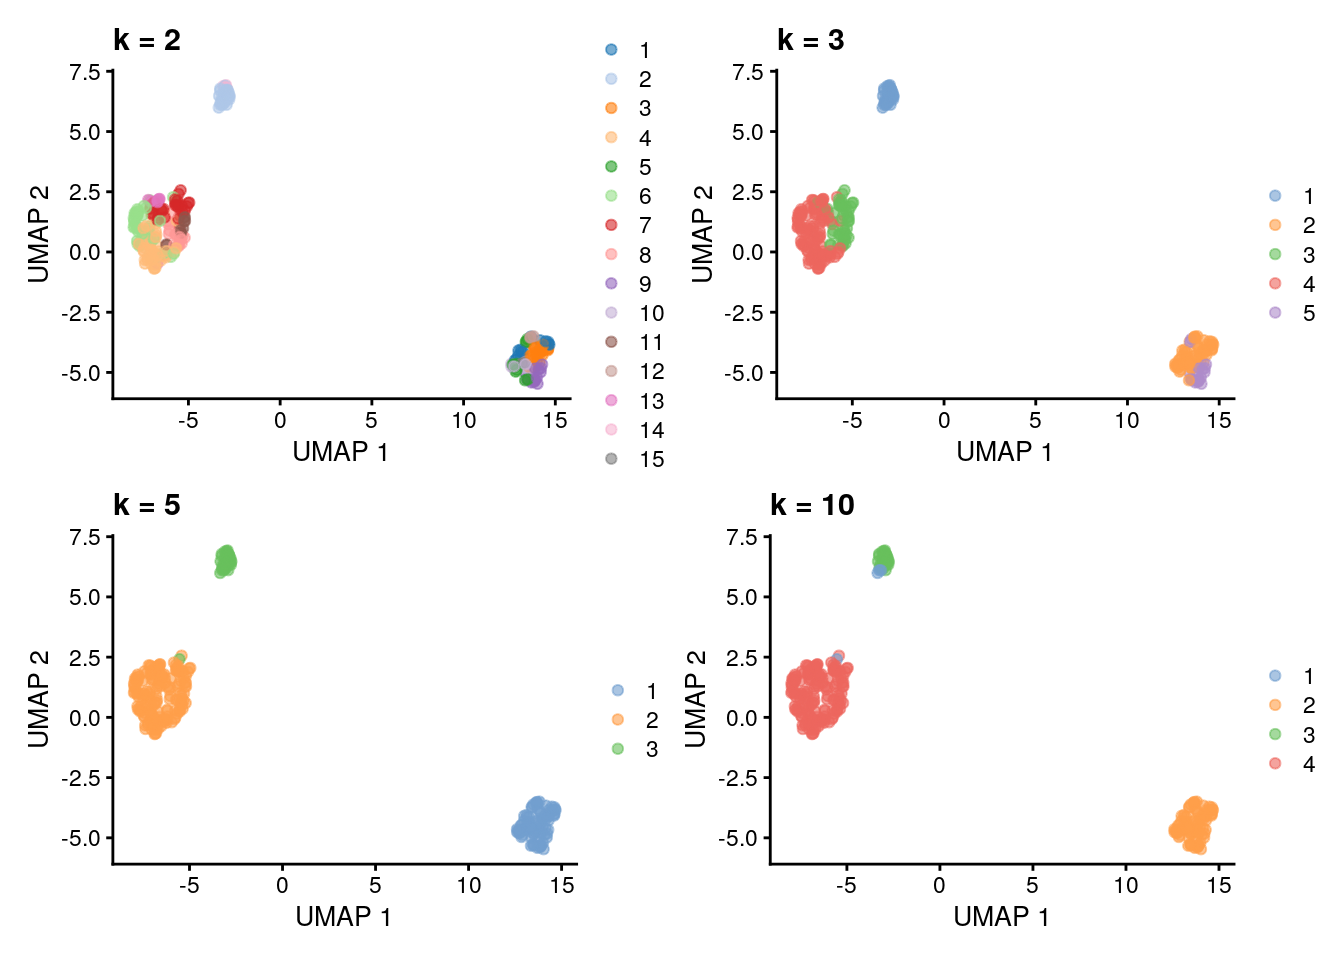
\includegraphics{21_microbiome_community_files/figure-latex/unnamed-chunk-15-1.pdf}

Similarly, the \emph{\texttt{bluster}} \citep{R-bluster} package offers clustering
diagnostics that can be used for judging the clustering quality (see
\href{http://bioconductor.org/packages/release/bioc/vignettes/bluster/inst/doc/diagnostics.html}{Assorted clustering
diagnostics}).
In the following, Silhouette width as a diagnostic tool is computed
and results are visualized for each case presented earlier. For more
about Silhouettes read \citep{Rousseeuw1987}.

\begin{Shaded}
\begin{Highlighting}[]
\NormalTok{ClustDiagPlot }\OtherTok{\textless{}{-}} \ControlFlowTok{function}\NormalTok{(x) \{}
  \CommentTok{\# Getting the clustering results}
\NormalTok{  graph\_clusters }\OtherTok{\textless{}{-}} \FunctionTok{clusterRows}\NormalTok{(}\FunctionTok{t}\NormalTok{(}\FunctionTok{assays}\NormalTok{(tse)}\SpecialCharTok{$}\NormalTok{rclr), }\FunctionTok{NNGraphParam}\NormalTok{(}\AttributeTok{k=}\NormalTok{x))}
  
  \CommentTok{\# Computing the diagnostic info}
\NormalTok{  sil }\OtherTok{\textless{}{-}} \FunctionTok{approxSilhouette}\NormalTok{(}\FunctionTok{t}\NormalTok{(}\FunctionTok{assays}\NormalTok{(tse)}\SpecialCharTok{$}\NormalTok{rclr), graph\_clusters)}
  
  \CommentTok{\# Plotting as a boxlpot to observe cluster separation}
  \FunctionTok{boxplot}\NormalTok{(}\FunctionTok{split}\NormalTok{(sil}\SpecialCharTok{$}\NormalTok{width, graph\_clusters), }\AttributeTok{main=}\FunctionTok{paste0}\NormalTok{(}\StringTok{"k = "}\NormalTok{, x))}
  
\NormalTok{\}}
\CommentTok{\# Applying the function for different k values}
\NormalTok{res }\OtherTok{\textless{}{-}} \FunctionTok{lapply}\NormalTok{(k,ClustDiagPlot)}
\end{Highlighting}
\end{Shaded}

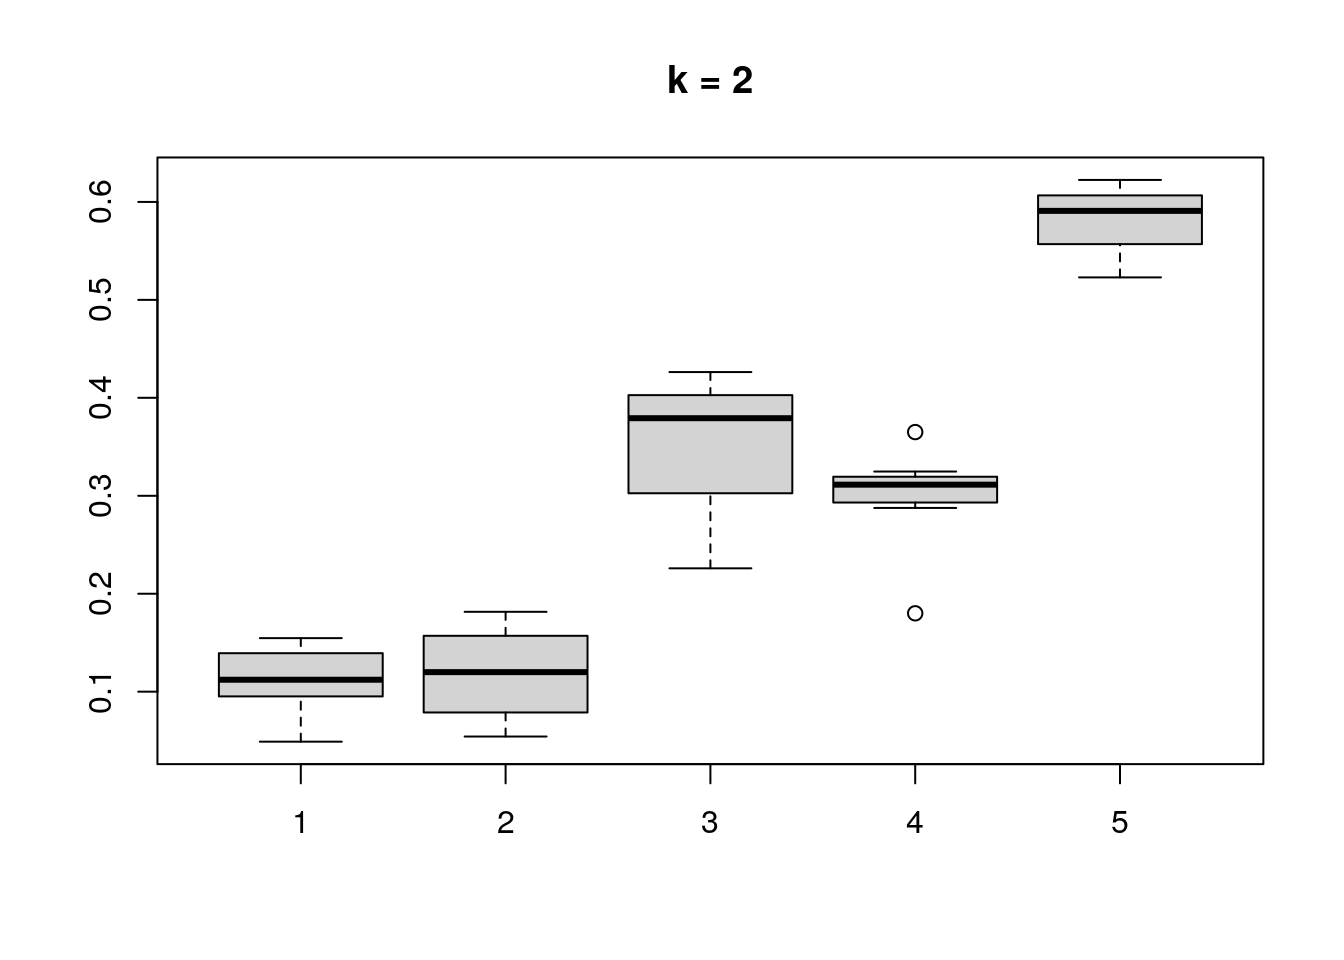
\includegraphics{21_microbiome_community_files/figure-latex/unnamed-chunk-16-1.pdf} 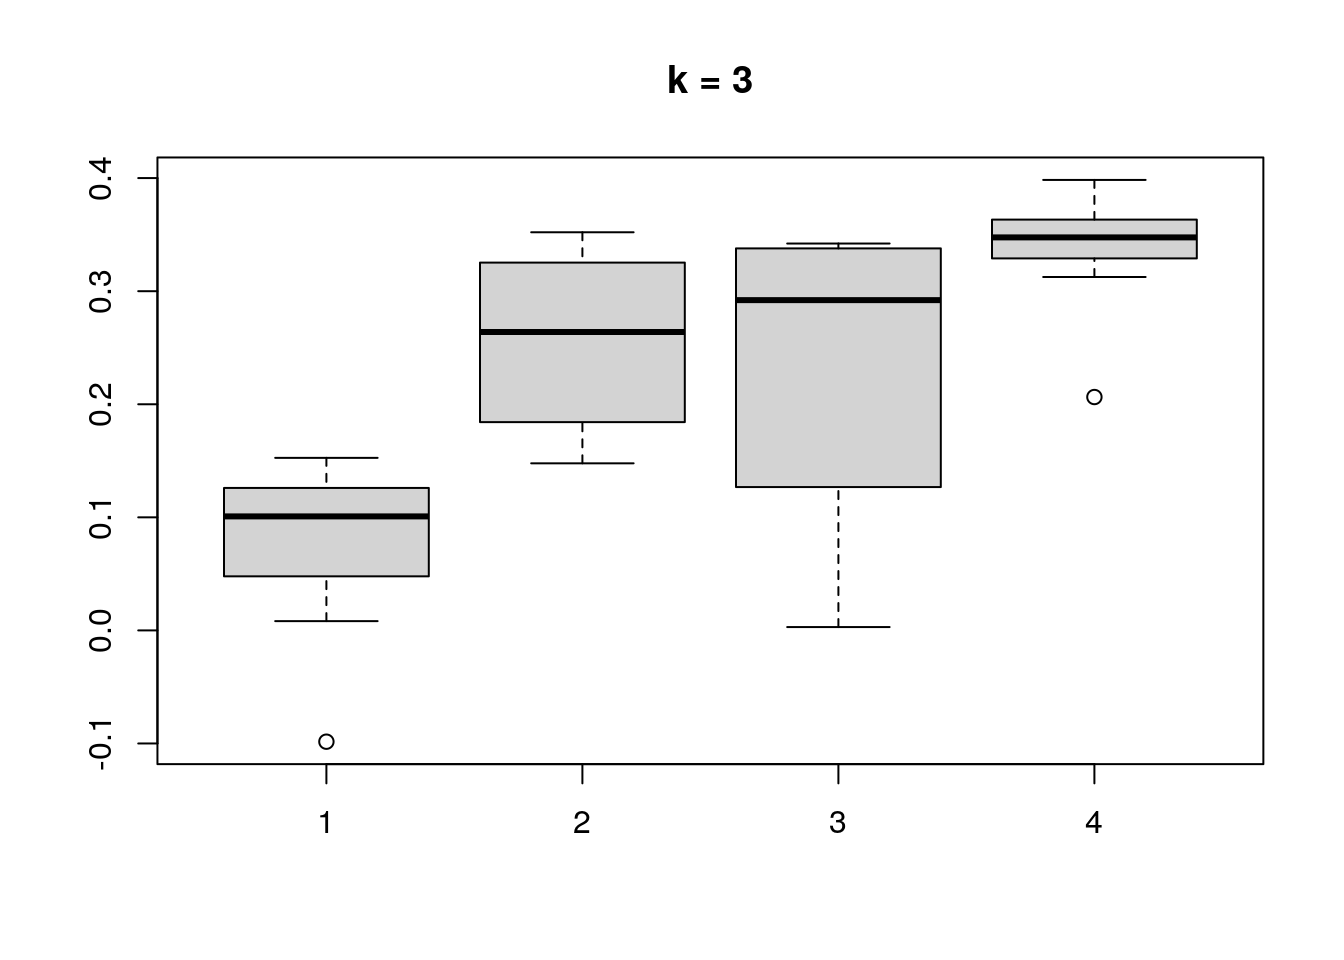
\includegraphics{21_microbiome_community_files/figure-latex/unnamed-chunk-16-2.pdf} 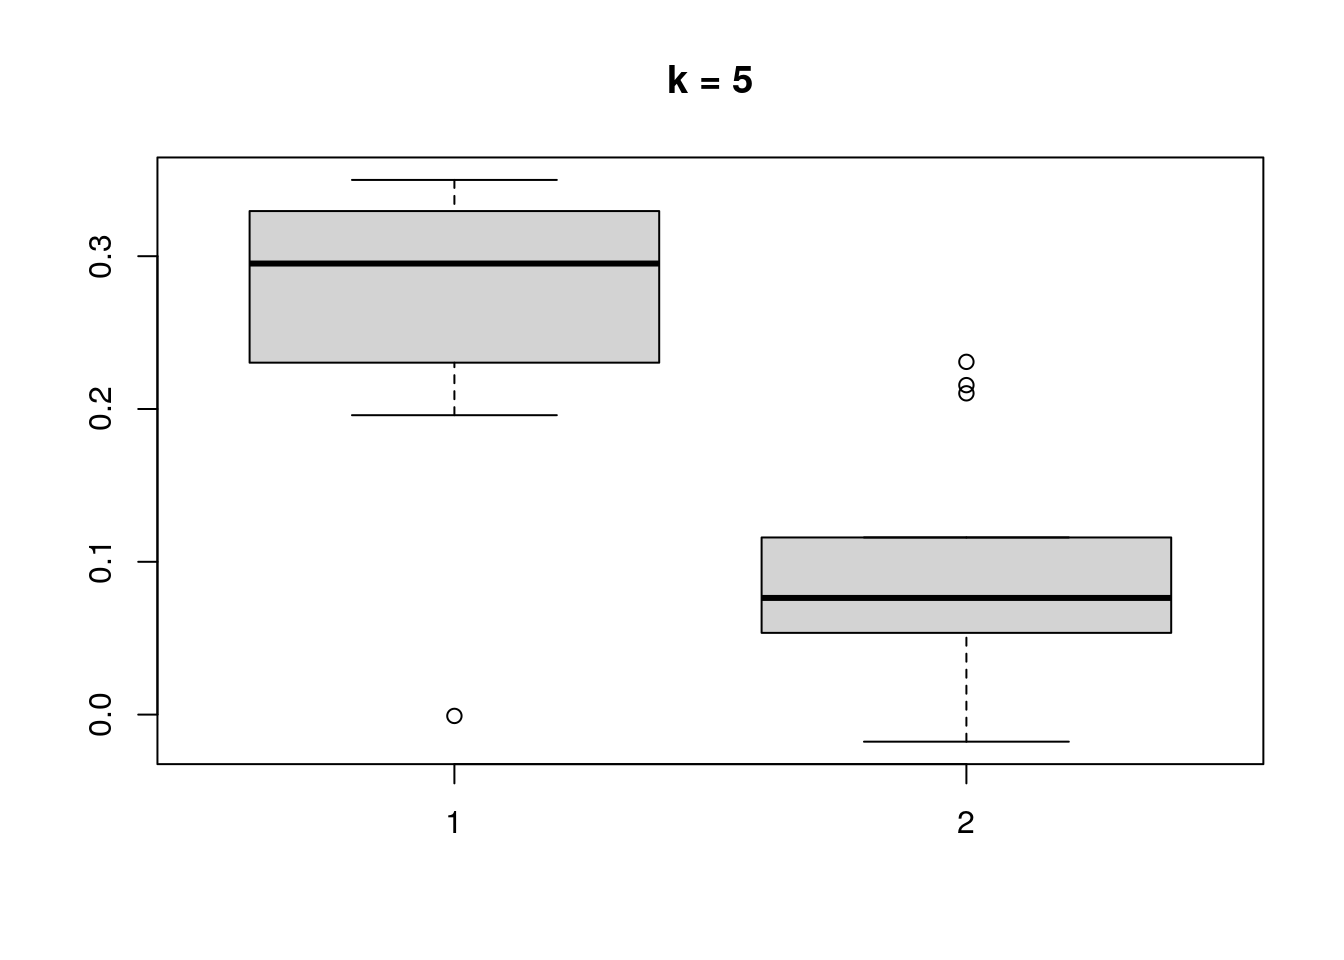
\includegraphics{21_microbiome_community_files/figure-latex/unnamed-chunk-16-3.pdf} 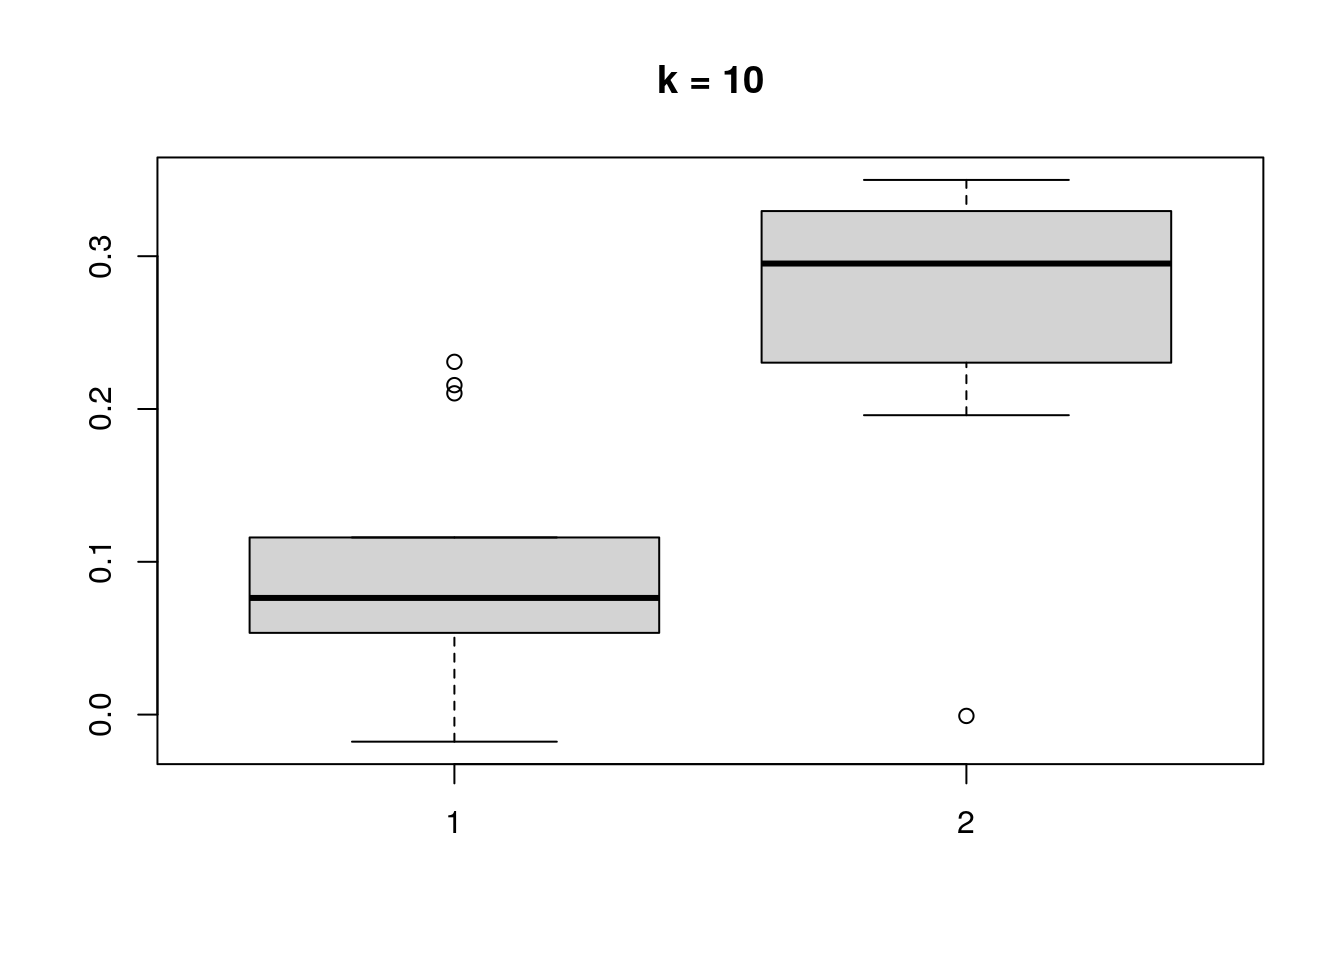
\includegraphics{21_microbiome_community_files/figure-latex/unnamed-chunk-16-4.pdf}

\hypertarget{additional-community-typing}{%
\section{Additional Community Typing}\label{additional-community-typing}}

For more community typing techniques applied to the `SprockettTHData' data set, see the attached .Rmd file.

Link:

\begin{itemize}
\tightlist
\item
  \href{add-comm-typing.Rmd}{Rmd}
\end{itemize}

\hypertarget{session-info-6}{%
\section*{Session Info}\label{session-info-6}}
\addcontentsline{toc}{section}{Session Info}

View session info

\begin{verbatim}
R version 4.1.2 (2021-11-01)
Platform: x86_64-pc-linux-gnu (64-bit)
Running under: Ubuntu 20.04.3 LTS

Matrix products: default
BLAS/LAPACK: /usr/lib/x86_64-linux-gnu/openblas-pthread/libopenblasp-r0.3.8.so

locale:
 [1] LC_CTYPE=en_US.UTF-8       LC_NUMERIC=C              
 [3] LC_TIME=en_US.UTF-8        LC_COLLATE=en_US.UTF-8    
 [5] LC_MONETARY=en_US.UTF-8    LC_MESSAGES=en_US.UTF-8   
 [7] LC_PAPER=en_US.UTF-8       LC_NAME=C                 
 [9] LC_ADDRESS=C               LC_TELEPHONE=C            
[11] LC_MEASUREMENT=en_US.UTF-8 LC_IDENTIFICATION=C       

attached base packages:
[1] stats4    stats     graphics  grDevices utils     datasets  methods  
[8] base     

other attached packages:
 [1] scater_1.22.0                  scuttle_1.4.0                 
 [3] bluster_1.4.0                  patchwork_1.1.1               
 [5] reshape2_1.4.4                 sechm_1.2.0                   
 [7] ggtree_3.2.1                   ape_5.6-2                     
 [9] pheatmap_1.0.12                miaViz_1.3.3                  
[11] ggraph_2.0.5                   ggplot2_3.3.5                 
[13] mia_1.3.19                     MultiAssayExperiment_1.20.0   
[15] TreeSummarizedExperiment_2.1.4 Biostrings_2.62.0             
[17] XVector_0.34.0                 SingleCellExperiment_1.16.0   
[19] SummarizedExperiment_1.24.0    Biobase_2.54.0                
[21] GenomicRanges_1.46.1           GenomeInfoDb_1.30.1           
[23] IRanges_2.28.0                 S4Vectors_0.32.3              
[25] BiocGenerics_0.40.0            MatrixGenerics_1.6.0          
[27] matrixStats_0.61.0-9001        ecodist_2.0.7                 
[29] BiocStyle_2.22.0               rebook_1.4.0                  

loaded via a namespace (and not attached):
  [1] circlize_0.4.14             plyr_1.8.6                 
  [3] igraph_1.2.11               lazyeval_0.2.2             
  [5] splines_4.1.2               BiocParallel_1.28.3        
  [7] digest_0.6.29               foreach_1.5.2              
  [9] yulab.utils_0.0.4           htmltools_0.5.2            
 [11] viridis_0.6.2               fansi_1.0.2                
 [13] magrittr_2.0.2              memoise_2.0.1              
 [15] ScaledMatrix_1.2.0          doParallel_1.0.17          
 [17] cluster_2.1.2               DECIPHER_2.22.0            
 [19] ComplexHeatmap_2.10.0       graphlayouts_0.8.0         
 [21] colorspace_2.0-3            blob_1.2.2                 
 [23] ggrepel_0.9.1               xfun_0.30                  
 [25] dplyr_1.0.8                 crayon_1.5.0               
 [27] RCurl_1.98-1.6              jsonlite_1.8.0             
 [29] graph_1.72.0                iterators_1.0.14           
 [31] glue_1.6.2                  polyclip_1.10-0            
 [33] registry_0.5-1              gtable_0.3.0               
 [35] zlibbioc_1.40.0             V8_4.1.0                   
 [37] GetoptLong_1.0.5            DelayedArray_0.20.0        
 [39] BiocSingular_1.10.0         shape_1.4.6                
 [41] scales_1.1.1                DBI_1.1.2                  
 [43] randomcoloR_1.1.0.1         Rcpp_1.0.8.3               
 [45] viridisLite_0.4.0           clue_0.3-60                
 [47] decontam_1.14.0             gridGraphics_0.5-1         
 [49] tidytree_0.3.9              bit_4.0.4                  
 [51] rsvd_1.0.5                  FNN_1.1.3                  
 [53] RColorBrewer_1.1-2          dir.expiry_1.2.0           
 [55] ellipsis_0.3.2              pkgconfig_2.0.3            
 [57] XML_3.99-0.9                farver_2.1.0               
 [59] uwot_0.1.11                 CodeDepends_0.6.5          
 [61] utf8_1.2.2                  ggplotify_0.1.0            
 [63] tidyselect_1.1.2            labeling_0.4.2             
 [65] rlang_1.0.2                 munsell_0.5.0              
 [67] tools_4.1.2                 cachem_1.0.6               
 [69] cli_3.2.0                   DirichletMultinomial_1.36.0
 [71] generics_0.1.2              RSQLite_2.2.10             
 [73] evaluate_0.15               stringr_1.4.0              
 [75] fastmap_1.1.0               yaml_2.3.5                 
 [77] knitr_1.37                  bit64_4.0.5                
 [79] tidygraph_1.2.0             purrr_0.3.4                
 [81] nlme_3.1-155                sparseMatrixStats_1.6.0    
 [83] aplot_0.1.2                 compiler_4.1.2             
 [85] curl_4.3.2                  png_0.1-7                  
 [87] beeswarm_0.4.0              filelock_1.0.2             
 [89] treeio_1.18.1               tibble_3.1.6               
 [91] tweenr_1.0.2                stringi_1.7.6              
 [93] highr_0.9                   lattice_0.20-45            
 [95] Matrix_1.4-0                vegan_2.5-7                
 [97] permute_0.9-7               vctrs_0.3.8                
 [99] pillar_1.7.0                lifecycle_1.0.1            
[101] BiocManager_1.30.16         GlobalOptions_0.1.2        
[103] BiocNeighbors_1.12.0        cowplot_1.1.1              
[105] bitops_1.0-7                irlba_2.3.5                
[107] seriation_1.3.3             R6_2.5.1                   
[109] TSP_1.2-0                   bookdown_0.25              
[111] gridExtra_2.3               vipor_0.4.5                
[113] codetools_0.2-18            MASS_7.3-55                
[115] assertthat_0.2.1            rjson_0.2.21               
[117] withr_2.5.0                 GenomeInfoDbData_1.2.7     
[119] mgcv_1.8-39                 parallel_4.1.2             
[121] grid_4.1.2                  ggfun_0.0.5                
[123] beachmat_2.10.0             tidyr_1.2.0                
[125] rmarkdown_2.13              DelayedMatrixStats_1.16.0  
[127] Rtsne_0.15                  ggnewscale_0.4.6           
[129] ggforce_0.3.3               ggbeeswarm_0.6.0           
\end{verbatim}

\hypertarget{biclustering}{%
\chapter{Biclustering}\label{biclustering}}

Biclustering is a clustering method, which simultaneously clusters rows and columns.
The idea is to find clusters where subset of features/samples share similar pattern
over samples/features.

There are multiple biclustering packages available, In this example, we use following methods
- \href{https://cran.r-project.org/web/packages/biclust/index.html}{biclust}
- \href{https://besjournals.onlinelibrary.wiley.com/doi/abs/10.1111/2041-210X.13582}{cobiclust}

\emph{cobiclust} is especially developed for microbiome data whereas \emph{biclust} is more
general method. In this section, we show three different cases and example
solutions to apply biclustering to them.

\begin{enumerate}
\def\labelenumi{\arabic{enumi}.}
\tightlist
\item
  Taxa vs samples
\item
  Taxa vs biomolecule/biomarker
\item
  Taxa vs taxa
\end{enumerate}

Biclusters can be visualized using heatmap or boxplot, for instance. For checking purposes,
also scatter plot might be valid choice.

Check more ideas for heatmaps from
\href{https://microbiome.github.io/OMA/microbiome-community.html\#composition-heatmap}{here}.

\hypertarget{taxa-vs-samples}{%
\section{Taxa vs samples}\label{taxa-vs-samples}}

When you have microbial abundance matrices, we suggest to use \emph{cobiclust} which is
designed for microbial data.

Load example data

\begin{Shaded}
\begin{Highlighting}[]
\FunctionTok{library}\NormalTok{(mia)}
\ControlFlowTok{if}\NormalTok{(}\SpecialCharTok{!}\FunctionTok{require}\NormalTok{(microbiomeDataSets))\{}
\NormalTok{    BiocManager}\SpecialCharTok{::}\FunctionTok{install}\NormalTok{(}\StringTok{"microbiomeDataSets"}\NormalTok{)}
    \FunctionTok{library}\NormalTok{(microbiomeDataSets)}
\NormalTok{\}}

\NormalTok{mae }\OtherTok{\textless{}{-}} \FunctionTok{HintikkaXOData}\NormalTok{()}

\NormalTok{mae}
\end{Highlighting}
\end{Shaded}

\begin{verbatim}
## A MultiAssayExperiment object of 3 listed
##  experiments with user-defined names and respective classes.
##  Containing an ExperimentList class object of length 3:
##  [1] microbiota: SummarizedExperiment with 12706 rows and 40 columns
##  [2] metabolites: SummarizedExperiment with 38 rows and 40 columns
##  [3] biomarkers: SummarizedExperiment with 39 rows and 40 columns
## Functionality:
##  experiments() - obtain the ExperimentList instance
##  colData() - the primary/phenotype DataFrame
##  sampleMap() - the sample coordination DataFrame
##  `$`, `[`, `[[` - extract colData columns, subset, or experiment
##  *Format() - convert into a long or wide DataFrame
##  assays() - convert ExperimentList to a SimpleList of matrices
##  exportClass() - save data to flat files
\end{verbatim}

Only the most prevalent taxa are included in analysis.

\begin{Shaded}
\begin{Highlighting}[]
\CommentTok{\# Subset data}
\NormalTok{mae[[}\DecValTok{1}\NormalTok{]] }\OtherTok{\textless{}{-}} \FunctionTok{subsetByPrevalentTaxa}\NormalTok{(mae[[}\DecValTok{1}\NormalTok{]], }\AttributeTok{rank =} \StringTok{"Genus"}\NormalTok{, }\AttributeTok{prevalence =} \FloatTok{0.2}\NormalTok{, }\AttributeTok{detection =} \FloatTok{0.001}\NormalTok{)}
\CommentTok{\# clr{-}transform}
\NormalTok{mae[[}\DecValTok{1}\NormalTok{]] }\OtherTok{\textless{}{-}} \FunctionTok{transformSamples}\NormalTok{(mae[[}\DecValTok{1}\NormalTok{]], }\AttributeTok{method =} \StringTok{"clr"}\NormalTok{, }\AttributeTok{pseudocount =} \DecValTok{1}\NormalTok{)}

\NormalTok{mae[[}\DecValTok{1}\NormalTok{]]}
\end{Highlighting}
\end{Shaded}

\begin{verbatim}
## class: SummarizedExperiment 
## dim: 57 40 
## metadata(1): agglomerated_by_rank
## assays(2): counts clr
## rownames(57): D_5__Escherichia-Shigella D_5__Ruminiclostridium 5 ...
##   D_5__[Ruminococcus] gauvreauii group D_5__Defluviitaleaceae UCG-011
## rowData names(7): Phylum Class ... Species OTU
## colnames(40): C1 C2 ... C39 C40
## colData names(0):
\end{verbatim}

\emph{cobiclust} takes counts table as an input and gives \emph{cobiclust} object as an output.
It includes clusters for taxa and samples.

\begin{Shaded}
\begin{Highlighting}[]
\ControlFlowTok{if}\NormalTok{(}\SpecialCharTok{!}\FunctionTok{require}\NormalTok{(cobiclust))\{}
    \FunctionTok{install.packages}\NormalTok{(}\StringTok{"cobiclust"}\NormalTok{)}
    \FunctionTok{library}\NormalTok{(cobiclust)}
\NormalTok{\}}

\CommentTok{\# Do clustering; use counts table´}
\NormalTok{clusters }\OtherTok{\textless{}{-}} \FunctionTok{cobiclust}\NormalTok{(}\FunctionTok{assay}\NormalTok{(mae[[}\DecValTok{1}\NormalTok{]], }\StringTok{"counts"}\NormalTok{))}

\CommentTok{\# Get clusters}
\NormalTok{row\_clusters }\OtherTok{\textless{}{-}}\NormalTok{ clusters}\SpecialCharTok{$}\NormalTok{classification}\SpecialCharTok{$}\NormalTok{rowclass}
\NormalTok{col\_clusters }\OtherTok{\textless{}{-}}\NormalTok{ clusters}\SpecialCharTok{$}\NormalTok{classification}\SpecialCharTok{$}\NormalTok{colclass}

\CommentTok{\# Add clusters to rowdata and coldata}
\FunctionTok{rowData}\NormalTok{(mae[[}\DecValTok{1}\NormalTok{]])}\SpecialCharTok{$}\NormalTok{clusters }\OtherTok{\textless{}{-}} \FunctionTok{factor}\NormalTok{(row\_clusters)}
\FunctionTok{colData}\NormalTok{(mae[[}\DecValTok{1}\NormalTok{]])}\SpecialCharTok{$}\NormalTok{clusters }\OtherTok{\textless{}{-}} \FunctionTok{factor}\NormalTok{(col\_clusters)}

\CommentTok{\# Order data based on clusters}
\NormalTok{mae[[}\DecValTok{1}\NormalTok{]] }\OtherTok{\textless{}{-}}\NormalTok{ mae[[}\DecValTok{1}\NormalTok{]][}\FunctionTok{order}\NormalTok{(}\FunctionTok{rowData}\NormalTok{(mae[[}\DecValTok{1}\NormalTok{]])}\SpecialCharTok{$}\NormalTok{clusters), }\FunctionTok{order}\NormalTok{(}\FunctionTok{colData}\NormalTok{(mae[[}\DecValTok{1}\NormalTok{]])}\SpecialCharTok{$}\NormalTok{clusters)]}

\CommentTok{\# Print clusters}
\NormalTok{clusters}\SpecialCharTok{$}\NormalTok{classification}
\end{Highlighting}
\end{Shaded}

\begin{verbatim}
## $rowclass
##  [1] 1 1 1 1 2 2 1 1 1 1 1 1 2 2 2 2 1 2 1 1 2 1 2 2 1 1 2 1 1 1 1 1 2 1 1 2 1 1
## [39] 1 1 1 1 1 1 1 1 1 2 1 2 1 1 1 2 1 1 1
## 
## $colclass
##  C1  C2  C3  C4  C5  C6  C7  C8  C9 C10 C11 C12 C13 C14 C15 C16 C17 C18 C19 C20 
##   1   2   2   2   2   2   2   2   2   2   2   2   2   2   2   2   2   2   2   2 
## C21 C22 C23 C24 C25 C26 C27 C28 C29 C30 C31 C32 C33 C34 C35 C36 C37 C38 C39 C40 
##   2   3   3   3   3   3   3   3   3   3   3   3   3   3   3   3   3   3   3   1
\end{verbatim}

Next we can plot clusters. Commonly used plot is heatmap with annotations.

\begin{Shaded}
\begin{Highlighting}[]
\ControlFlowTok{if}\NormalTok{(}\SpecialCharTok{!}\FunctionTok{require}\NormalTok{(pheatmap))\{}
    \FunctionTok{install.packages}\NormalTok{(}\StringTok{"pheatmap"}\NormalTok{)}
    \FunctionTok{library}\NormalTok{(pheatmap)}
\NormalTok{\}}
\CommentTok{\# z{-}transform for heatmap}
\NormalTok{mae[[}\DecValTok{1}\NormalTok{]] }\OtherTok{\textless{}{-}} \FunctionTok{transformFeatures}\NormalTok{(mae[[}\DecValTok{1}\NormalTok{]], }\AttributeTok{abund\_values =} \StringTok{"clr"}\NormalTok{, }\AttributeTok{method =} \StringTok{"z"}\NormalTok{, }\AttributeTok{name =} \StringTok{"clr\_z"}\NormalTok{)}

\CommentTok{\# Create annotations. When column names are equal, they should share levels. }
\CommentTok{\# Here samples include 3 clusters, and taxa 2. That is why we have to make }
\CommentTok{\# column names unique. }
\NormalTok{annotation\_col }\OtherTok{\textless{}{-}} \FunctionTok{data.frame}\NormalTok{(}\FunctionTok{colData}\NormalTok{(mae[[}\DecValTok{1}\NormalTok{]])[, }\StringTok{"clusters"}\NormalTok{, }\AttributeTok{drop =}\NormalTok{ F])}
\FunctionTok{colnames}\NormalTok{(annotation\_col) }\OtherTok{\textless{}{-}} \StringTok{"col\_clusters"}

\NormalTok{annotation\_row }\OtherTok{\textless{}{-}} \FunctionTok{data.frame}\NormalTok{(}\FunctionTok{rowData}\NormalTok{(mae[[}\DecValTok{1}\NormalTok{]])[, }\StringTok{"clusters"}\NormalTok{, }\AttributeTok{drop =}\NormalTok{ F])}
\FunctionTok{colnames}\NormalTok{(annotation\_row) }\OtherTok{\textless{}{-}} \StringTok{"row\_clusters"}

\CommentTok{\# Create a heatmap}
\FunctionTok{pheatmap}\NormalTok{(}\FunctionTok{assay}\NormalTok{(mae[[}\DecValTok{1}\NormalTok{]], }\StringTok{"clr\_z"}\NormalTok{), }\AttributeTok{cluster\_rows =}\NormalTok{ F, }\AttributeTok{cluster\_cols =}\NormalTok{ F, }
         \AttributeTok{annotation\_col =}\NormalTok{ annotation\_col,}
         \AttributeTok{annotation\_row =}\NormalTok{ annotation\_row)}
\end{Highlighting}
\end{Shaded}

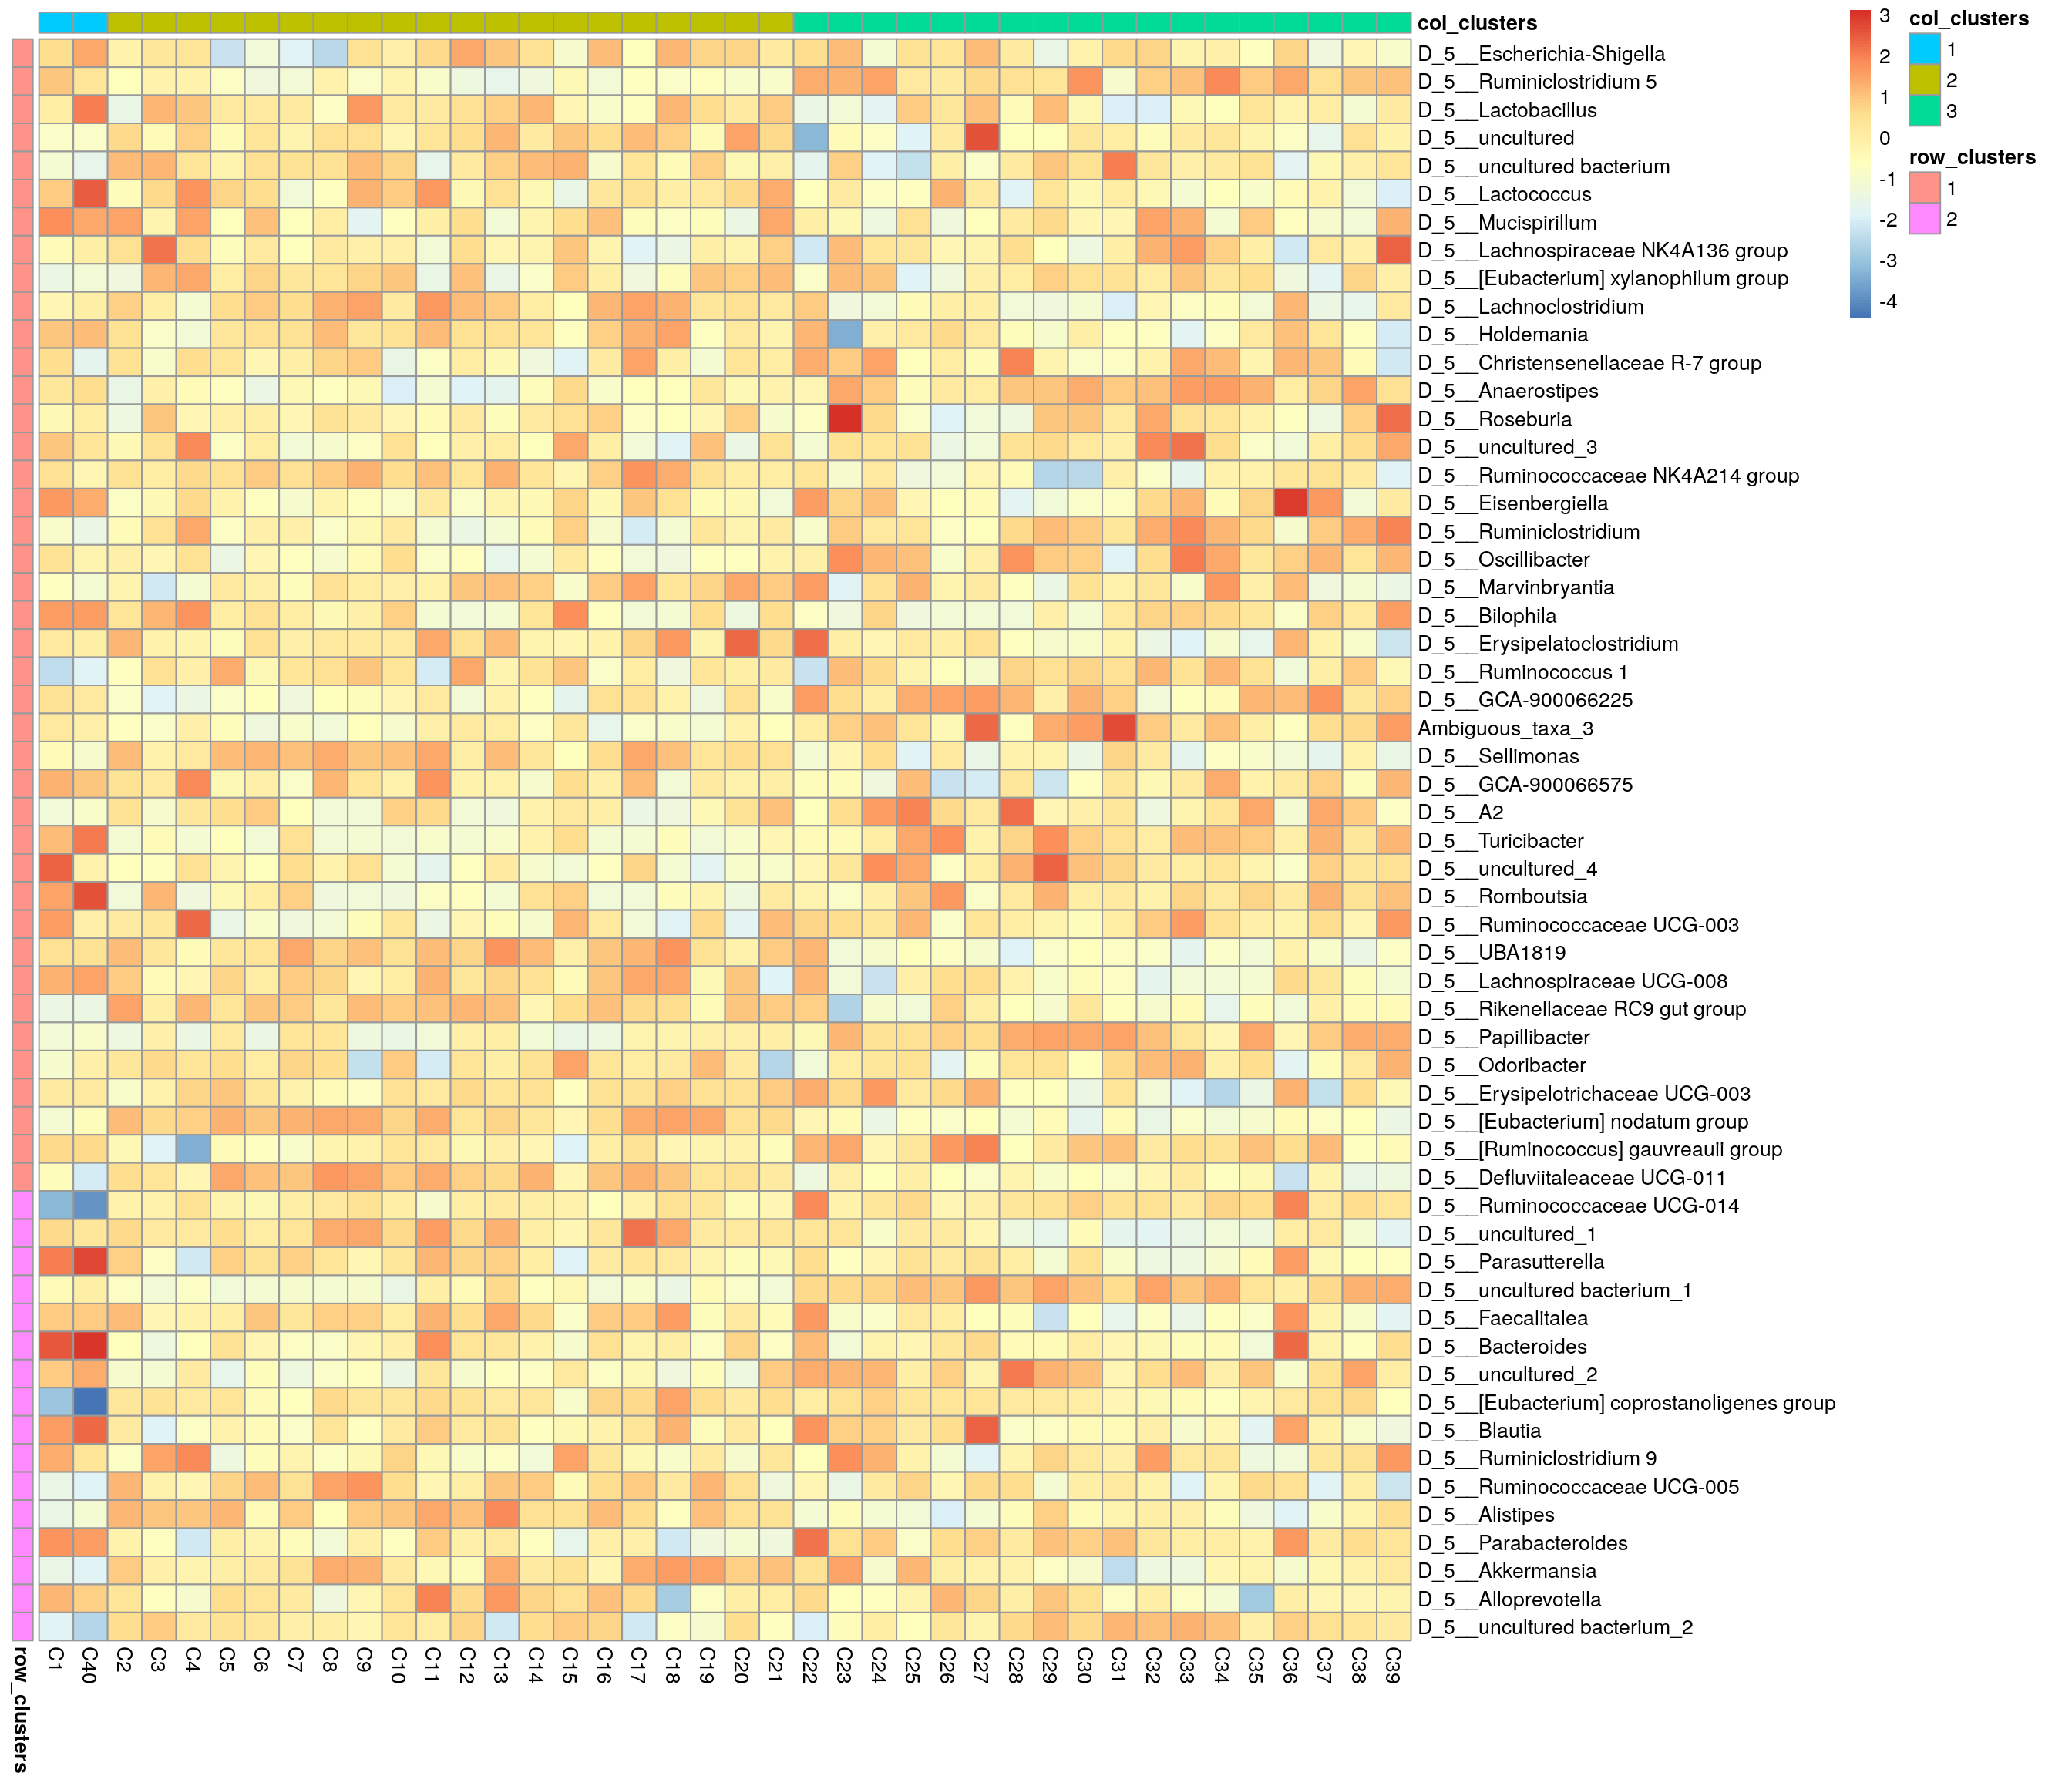
\includegraphics{24_biclustering_files/figure-latex/cobiclust_3-1.pdf}

Another common plot is a boxplot.

\begin{Shaded}
\begin{Highlighting}[]
\ControlFlowTok{if}\NormalTok{(}\SpecialCharTok{!}\FunctionTok{require}\NormalTok{(ggplot2))\{}
    \FunctionTok{install.packages}\NormalTok{(}\StringTok{"ggplot2"}\NormalTok{)}
    \FunctionTok{library}\NormalTok{(ggplot2)}
\NormalTok{\}}
\ControlFlowTok{if}\NormalTok{(}\SpecialCharTok{!}\FunctionTok{require}\NormalTok{(patchwork))\{}
    \FunctionTok{install.packages}\NormalTok{(}\StringTok{"patchwork"}\NormalTok{)}
    \FunctionTok{library}\NormalTok{(patchwork)}
\NormalTok{\}}

\CommentTok{\# ggplot requires data in melted format}
\NormalTok{melt\_assay }\OtherTok{\textless{}{-}} \FunctionTok{meltAssay}\NormalTok{(mae[[}\DecValTok{1}\NormalTok{]], }\AttributeTok{abund\_values =} \StringTok{"clr"}\NormalTok{, }\AttributeTok{add\_col\_data =}\NormalTok{ T, }\AttributeTok{add\_row\_data =}\NormalTok{ T)}

\CommentTok{\# patchwork two plots side{-}by{-}side}
\NormalTok{p1 }\OtherTok{\textless{}{-}} \FunctionTok{ggplot}\NormalTok{(melt\_assay) }\SpecialCharTok{+}
  \FunctionTok{geom\_boxplot}\NormalTok{(}\FunctionTok{aes}\NormalTok{(}\AttributeTok{x =}\NormalTok{ clusters.x, }\AttributeTok{y =}\NormalTok{ clr)) }\SpecialCharTok{+}
  \FunctionTok{labs}\NormalTok{(}\AttributeTok{x =} \StringTok{"Taxa clusters"}\NormalTok{)}
\NormalTok{p2 }\OtherTok{\textless{}{-}} \FunctionTok{ggplot}\NormalTok{(melt\_assay) }\SpecialCharTok{+}
  \FunctionTok{geom\_boxplot}\NormalTok{(}\FunctionTok{aes}\NormalTok{(}\AttributeTok{x =}\NormalTok{ clusters.y, }\AttributeTok{y =}\NormalTok{ clr)) }\SpecialCharTok{+}
  \FunctionTok{labs}\NormalTok{(}\AttributeTok{x =} \StringTok{"Sample clusters"}\NormalTok{)}

\NormalTok{p1 }\SpecialCharTok{+}\NormalTok{ p2}
\end{Highlighting}
\end{Shaded}

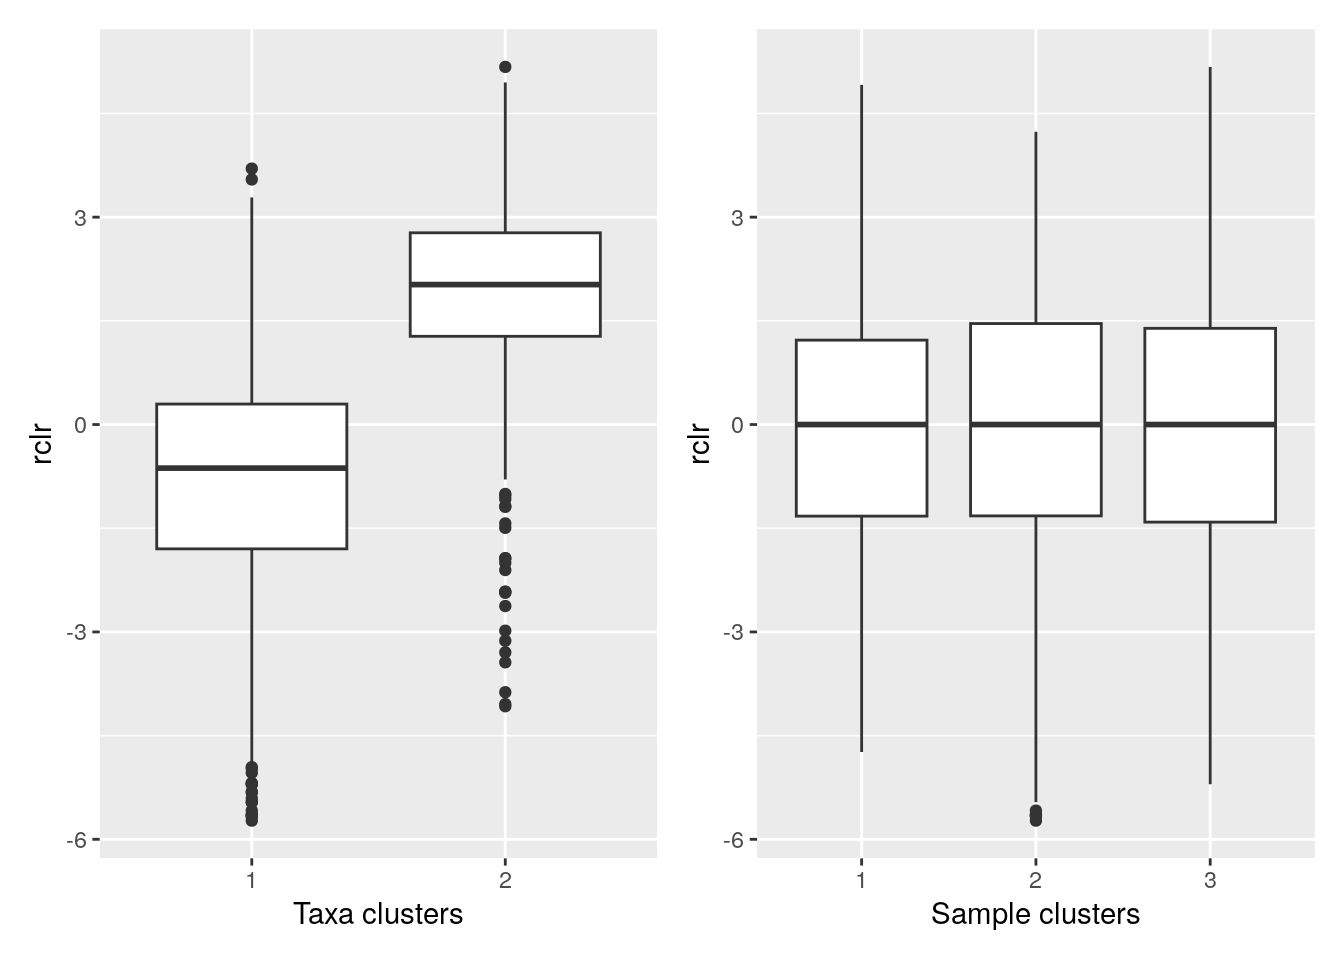
\includegraphics{24_biclustering_files/figure-latex/cobiclust_4-1.pdf}

\hypertarget{taxa-vs-biomolecules}{%
\section{Taxa vs biomolecules}\label{taxa-vs-biomolecules}}

Here, we analyze cross-correlation between taxa and metabolites. This is a case, where
we use \emph{biclust} method which is suitable for numeric matrices in general.

\begin{Shaded}
\begin{Highlighting}[]
\DocumentationTok{\#\#\#\#\#\#\#\#\#\#\#\#\#\#\#\#\#\#\#\#\#\#\#\#\#\#\#\# REMOVE THIS WHEN }\AlertTok{BUG}\DocumentationTok{ IN GETEXPERIMENTCROSSCORR IS FIXED}
\FunctionTok{rownames}\NormalTok{(mae[[}\DecValTok{1}\NormalTok{]]) }\OtherTok{\textless{}{-}} \FunctionTok{make.unique}\NormalTok{(}\FunctionTok{rownames}\NormalTok{(mae[[}\DecValTok{1}\NormalTok{]]))}

\CommentTok{\# Calculate correlations}
\NormalTok{corr }\OtherTok{\textless{}{-}} \FunctionTok{getExperimentCrossCorrelation}\NormalTok{(mae, }\DecValTok{1}\NormalTok{, }\DecValTok{2}\NormalTok{, }
                                      \AttributeTok{abund\_values1 =} \StringTok{"clr"}\NormalTok{, }
                                      \AttributeTok{abund\_values2 =} \StringTok{"nmr"}\NormalTok{, }
                                      \AttributeTok{mode =} \StringTok{"matrix"}\NormalTok{, }
                                      \AttributeTok{cor\_threshold =} \FloatTok{0.2}\NormalTok{)}
\end{Highlighting}
\end{Shaded}

\emph{biclust} takes matrix as an input and returns \emph{biclust} object.

\begin{Shaded}
\begin{Highlighting}[]
\CommentTok{\# Load package}
\ControlFlowTok{if}\NormalTok{(}\SpecialCharTok{!}\FunctionTok{require}\NormalTok{(biclust))\{}
    \FunctionTok{install.packages}\NormalTok{(}\StringTok{"biclust"}\NormalTok{)}
    \FunctionTok{library}\NormalTok{(biclust)}
\NormalTok{\}}

\CommentTok{\# Set seed for reproducibility}
\FunctionTok{set.seed}\NormalTok{(}\DecValTok{3973}\NormalTok{)}

\CommentTok{\# Find biclusters}
\NormalTok{bc }\OtherTok{\textless{}{-}} \FunctionTok{biclust}\NormalTok{(corr, }\AttributeTok{method=}\FunctionTok{BCPlaid}\NormalTok{(), }\AttributeTok{fit.model =}\NormalTok{ y }\SpecialCharTok{\textasciitilde{}}\NormalTok{ m,}
              \AttributeTok{background =} \ConstantTok{TRUE}\NormalTok{, }\AttributeTok{shuffle =} \DecValTok{100}\NormalTok{, }\AttributeTok{back.fit =} \DecValTok{0}\NormalTok{, }\AttributeTok{max.layers =} \DecValTok{10}\NormalTok{,}
              \AttributeTok{iter.startup =} \DecValTok{10}\NormalTok{, }\AttributeTok{iter.layer =} \DecValTok{100}\NormalTok{, }\AttributeTok{verbose =} \ConstantTok{FALSE}\NormalTok{)}

\NormalTok{bc}
\end{Highlighting}
\end{Shaded}

\begin{verbatim}
## 
## An object of class Biclust 
## 
## call:
##  biclust(x = corr, method = BCPlaid(), fit.model = y ~ m, background = TRUE, 
##      shuffle = 100, back.fit = 0, max.layers = 10, iter.startup = 10, 
##      iter.layer = 100, verbose = FALSE)
## 
## Number of Clusters found:  2 
## 
## First  2  Cluster sizes:
##                    BC 1 BC 2
## Number of Rows:       8    3
## Number of Columns:    7    8
\end{verbatim}

The object includes cluster information. However compared to \emph{cobiclust},
\emph{biclust} object includes only information about clusters that were found, not general cluster.

Meaning that if one cluster size of 5 features was found out of 20 features,
those 15 features do not belong to any cluster. That is why we have to create an
additional cluster for features/samples that are not assigned into any cluster.

\begin{Shaded}
\begin{Highlighting}[]
\CommentTok{\# Functions for obtaining biclust information}

\CommentTok{\# Get clusters for rows and columns}
\NormalTok{.get\_biclusters\_from\_biclust }\OtherTok{\textless{}{-}} \ControlFlowTok{function}\NormalTok{(bc, assay)\{}
  \CommentTok{\# Get cluster information for columns and rows}
\NormalTok{  bc\_columns }\OtherTok{\textless{}{-}} \FunctionTok{t}\NormalTok{(bc}\SpecialCharTok{@}\NormalTok{NumberxCol)}
\NormalTok{  bc\_columns }\OtherTok{\textless{}{-}} \FunctionTok{data.frame}\NormalTok{(bc\_columns)}
\NormalTok{  bc\_rows }\OtherTok{\textless{}{-}}\NormalTok{ bc}\SpecialCharTok{@}\NormalTok{RowxNumber}
\NormalTok{  bc\_rows }\OtherTok{\textless{}{-}} \FunctionTok{data.frame}\NormalTok{(bc\_rows)}
  
  \CommentTok{\# Get data into right format}
\NormalTok{  bc\_columns }\OtherTok{\textless{}{-}} \FunctionTok{.manipulate\_bc\_data}\NormalTok{(bc\_columns, assay, }\StringTok{"col"}\NormalTok{)}
\NormalTok{  bc\_rows }\OtherTok{\textless{}{-}} \FunctionTok{.manipulate\_bc\_data}\NormalTok{(bc\_rows, assay, }\StringTok{"row"}\NormalTok{)}
  
  \FunctionTok{return}\NormalTok{(}\FunctionTok{list}\NormalTok{(}\AttributeTok{bc\_columns =}\NormalTok{ bc\_columns, }\AttributeTok{bc\_rows =}\NormalTok{ bc\_rows))}
\NormalTok{\}}

\CommentTok{\# Input clusters, and how many observations there should be, i.e., the number of samples or features}
\NormalTok{.manipulate\_bc\_data }\OtherTok{\textless{}{-}} \ControlFlowTok{function}\NormalTok{(bc\_clusters, assay, row\_col)\{}
  \CommentTok{\# Get right dimension}
\NormalTok{  dim }\OtherTok{\textless{}{-}} \FunctionTok{ifelse}\NormalTok{(row\_col }\SpecialCharTok{==} \StringTok{"col"}\NormalTok{, }\FunctionTok{ncol}\NormalTok{(assay), }\FunctionTok{nrow}\NormalTok{(assay))}
  \CommentTok{\# Get column/row names}
  \ControlFlowTok{if}\NormalTok{( row\_col }\SpecialCharTok{==} \StringTok{"col"}\NormalTok{ )\{}
\NormalTok{    names }\OtherTok{\textless{}{-}} \FunctionTok{colnames}\NormalTok{(assay)}
\NormalTok{  \} }\ControlFlowTok{else}\NormalTok{\{}
\NormalTok{    names }\OtherTok{\textless{}{-}} \FunctionTok{rownames}\NormalTok{(assay)}
\NormalTok{  \}}
  
  \CommentTok{\# If no clusters were found, create one. Otherwise create additional cluster which}
  \CommentTok{\# contain those samples that are not included in clusters that were found.}
  \ControlFlowTok{if}\NormalTok{( }\FunctionTok{nrow}\NormalTok{(bc\_clusters) }\SpecialCharTok{!=}\NormalTok{ dim )\{}
\NormalTok{      bc\_clusters }\OtherTok{\textless{}{-}} \FunctionTok{data.frame}\NormalTok{(}\AttributeTok{cluster =} \FunctionTok{rep}\NormalTok{(}\ConstantTok{TRUE}\NormalTok{, dim))}
\NormalTok{  \} }\ControlFlowTok{else}\NormalTok{ \{}
      \CommentTok{\# Create additional cluster that includes those samples/features that}
      \CommentTok{\# are not included in other clusters.}
\NormalTok{      vec }\OtherTok{\textless{}{-}} \FunctionTok{ifelse}\NormalTok{(}\FunctionTok{rowSums}\NormalTok{(bc\_clusters) }\SpecialCharTok{\textgreater{}} \DecValTok{0}\NormalTok{, }\ConstantTok{FALSE}\NormalTok{, }\ConstantTok{TRUE}\NormalTok{)}
      \CommentTok{\# If additional cluster contains samples, then add it}
      \ControlFlowTok{if}\NormalTok{ ( }\FunctionTok{any}\NormalTok{(vec) )\{}
\NormalTok{          bc\_clusters }\OtherTok{\textless{}{-}} \FunctionTok{cbind}\NormalTok{(bc\_clusters, vec)}
\NormalTok{      \}}
\NormalTok{  \}}
  \CommentTok{\# Adjust row and column names}
  \FunctionTok{rownames}\NormalTok{(bc\_clusters) }\OtherTok{\textless{}{-}}\NormalTok{ names}
  \FunctionTok{colnames}\NormalTok{(bc\_clusters) }\OtherTok{\textless{}{-}} \FunctionTok{paste0}\NormalTok{(}\StringTok{"cluster\_"}\NormalTok{, }\DecValTok{1}\SpecialCharTok{:}\FunctionTok{ncol}\NormalTok{(bc\_clusters))}
  \FunctionTok{return}\NormalTok{(bc\_clusters)}
\NormalTok{\}}
\end{Highlighting}
\end{Shaded}

\begin{Shaded}
\begin{Highlighting}[]
\CommentTok{\# Get biclusters}
\NormalTok{bcs }\OtherTok{\textless{}{-}} \FunctionTok{.get\_biclusters\_from\_biclust}\NormalTok{(bc, corr)}

\NormalTok{bicluster\_rows }\OtherTok{\textless{}{-}}\NormalTok{ bcs}\SpecialCharTok{$}\NormalTok{bc\_rows}
\NormalTok{bicluster\_columns }\OtherTok{\textless{}{-}}\NormalTok{ bcs}\SpecialCharTok{$}\NormalTok{bc\_columns}

\CommentTok{\# Print biclusters for rows}
\FunctionTok{head}\NormalTok{(bicluster\_rows)}
\end{Highlighting}
\end{Shaded}

\begin{verbatim}
##                           cluster_1 cluster_2 cluster_3
## D_5__Escherichia-Shigella     FALSE     FALSE      TRUE
## D_5__Ruminiclostridium 5       TRUE     FALSE     FALSE
## D_5__Lactobacillus            FALSE     FALSE      TRUE
## D_5__uncultured               FALSE     FALSE      TRUE
## D_5__uncultured bacterium     FALSE     FALSE      TRUE
## D_5__Lactococcus              FALSE     FALSE      TRUE
\end{verbatim}

Let's collect information for the scatter plot.

\begin{Shaded}
\begin{Highlighting}[]
\CommentTok{\# Function for obtaining sample{-}wise sum, mean, median, and mean variance for each cluster}
\NormalTok{.sum\_mean\_median\_var }\OtherTok{\textless{}{-}} \ControlFlowTok{function}\NormalTok{(tse1, tse2, abund\_values1, abund\_values2, clusters1, clusters2)\{}
  
\NormalTok{  list }\OtherTok{\textless{}{-}} \FunctionTok{list}\NormalTok{()}
  \CommentTok{\# Create a data frame that includes all the information}
  \ControlFlowTok{for}\NormalTok{(i }\ControlFlowTok{in} \DecValTok{1}\SpecialCharTok{:}\FunctionTok{ncol}\NormalTok{(clusters1) )\{}
    \CommentTok{\# Subset data based on cluster}
\NormalTok{    tse\_subset1 }\OtherTok{\textless{}{-}}\NormalTok{ tse1[clusters1[,i], ]}
\NormalTok{    tse\_subset2 }\OtherTok{\textless{}{-}}\NormalTok{ tse2[clusters2[,i], ]}
    \CommentTok{\# Get assay}
\NormalTok{    assay1 }\OtherTok{\textless{}{-}} \FunctionTok{assay}\NormalTok{(tse\_subset1, abund\_values1)}
\NormalTok{    assay2 }\OtherTok{\textless{}{-}} \FunctionTok{assay}\NormalTok{(tse\_subset2, abund\_values2)}
    \CommentTok{\# Calculate sum, mean, median, and mean variance}
\NormalTok{    sum1 }\OtherTok{\textless{}{-}} \FunctionTok{colSums2}\NormalTok{(assay1, }\AttributeTok{na.rm =}\NormalTok{ T)}
\NormalTok{    mean1 }\OtherTok{\textless{}{-}} \FunctionTok{colMeans2}\NormalTok{(assay1, }\AttributeTok{na.rm =}\NormalTok{ T)}
\NormalTok{    median1 }\OtherTok{\textless{}{-}} \FunctionTok{colMedians}\NormalTok{(assay1, }\AttributeTok{na.rm =}\NormalTok{ T)}
\NormalTok{    var1 }\OtherTok{\textless{}{-}} \FunctionTok{colVars}\NormalTok{(assay1, }\AttributeTok{na.rm =}\NormalTok{ T)}
    
\NormalTok{    sum2 }\OtherTok{\textless{}{-}} \FunctionTok{colSums2}\NormalTok{(assay2, }\AttributeTok{na.rm =}\NormalTok{ T)}
\NormalTok{    mean2 }\OtherTok{\textless{}{-}} \FunctionTok{colMeans2}\NormalTok{(assay2, }\AttributeTok{na.rm =}\NormalTok{ T)}
\NormalTok{    median2 }\OtherTok{\textless{}{-}} \FunctionTok{colMedians}\NormalTok{(assay2, }\AttributeTok{na.rm =}\NormalTok{ T)}
\NormalTok{    var2 }\OtherTok{\textless{}{-}} \FunctionTok{colVars}\NormalTok{(assay2, }\AttributeTok{na.rm =}\NormalTok{ T)}
    
\NormalTok{    list[[i]] }\OtherTok{\textless{}{-}} \FunctionTok{data.frame}\NormalTok{(}\AttributeTok{sample =} \FunctionTok{colnames}\NormalTok{(tse1), sum1, sum2, mean1, mean2, }
\NormalTok{                     median1, median2, var1, var2)}
\NormalTok{  \}}

  \FunctionTok{return}\NormalTok{(list)}
\NormalTok{\}}

\CommentTok{\# Calculate info}
\NormalTok{df }\OtherTok{\textless{}{-}} \FunctionTok{.sum\_mean\_median\_var}\NormalTok{(mae[[}\DecValTok{1}\NormalTok{]], mae[[}\DecValTok{2}\NormalTok{]], }\StringTok{"clr"}\NormalTok{, }\StringTok{"nmr"}\NormalTok{, bicluster\_rows, bicluster\_columns)}
\end{Highlighting}
\end{Shaded}

Now we can create a scatter plot. X-axis includes median clr abundance of microbiome
and y-axis median absolute concentration of each metabolite. Each data point represents
a single sample.

From the plots, we can see that there is low negative correlation in both cluster 1 and 3.
This means that when abundance of bacteria belonging to cluster 1 or 3 is higher,
the concentration of metabolites of cluster 1 or 3 is lower, and vice versa.

\begin{Shaded}
\begin{Highlighting}[]
\NormalTok{plot\_list }\OtherTok{\textless{}{-}} \FunctionTok{list}\NormalTok{()}

\NormalTok{i }\OtherTok{\textless{}{-}} \DecValTok{0}
\ControlFlowTok{for}\NormalTok{( data }\ControlFlowTok{in}\NormalTok{ df )\{}
\NormalTok{  i }\OtherTok{\textless{}{-}}\NormalTok{ i }\SpecialCharTok{+}\DecValTok{1}
\NormalTok{  plot\_list[[i]] }\OtherTok{\textless{}{-}} \FunctionTok{ggplot}\NormalTok{(data)  }\SpecialCharTok{+}
      \FunctionTok{geom\_point}\NormalTok{(}\FunctionTok{aes}\NormalTok{(}\AttributeTok{x =}\NormalTok{ median1, }\AttributeTok{y =}\NormalTok{ median2)) }\SpecialCharTok{+} 
    \FunctionTok{labs}\NormalTok{(}\AttributeTok{title =} \FunctionTok{paste0}\NormalTok{(}\StringTok{"Cluster "}\NormalTok{, i), }\AttributeTok{x =} \StringTok{"Taxa (clr median)"}\NormalTok{, }\AttributeTok{y =} \StringTok{"Metabolites (abs. median)"}\NormalTok{)}
\NormalTok{\}}

\NormalTok{plot\_list[[}\DecValTok{1}\NormalTok{]] }\SpecialCharTok{+}\NormalTok{ plot\_list[[}\DecValTok{2}\NormalTok{]] }\SpecialCharTok{+}\NormalTok{ plot\_list[[}\DecValTok{3}\NormalTok{]]}
\end{Highlighting}
\end{Shaded}

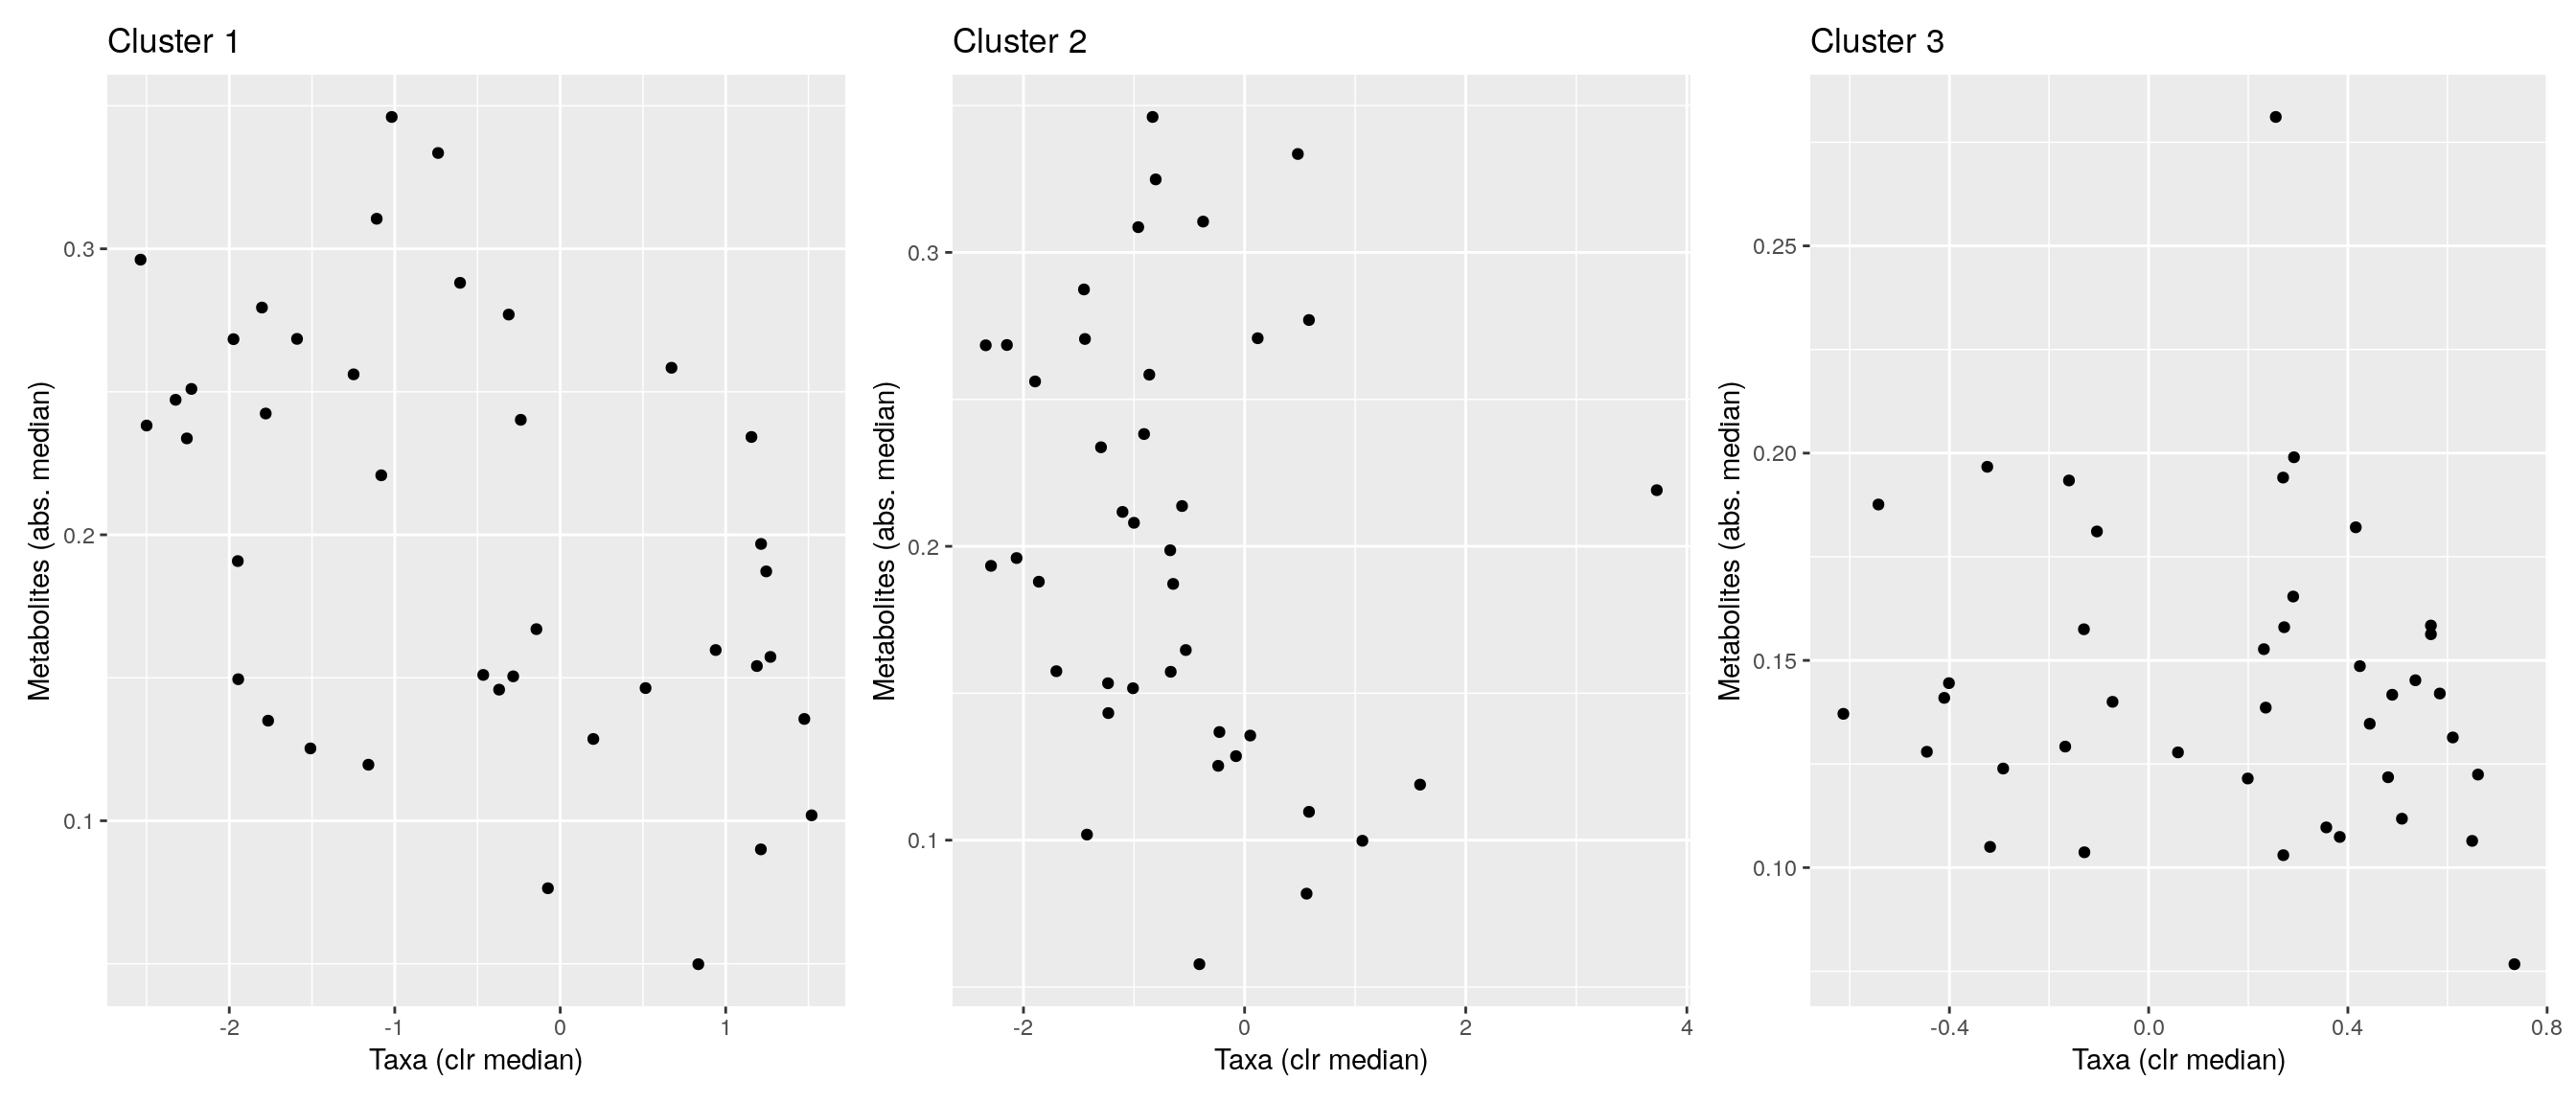
\includegraphics{24_biclustering_files/figure-latex/biclust_6-1.pdf}

\emph{pheatmap} does not allow boolean values, so they must be converted into factors.

\begin{Shaded}
\begin{Highlighting}[]
\NormalTok{bicluster\_columns }\OtherTok{\textless{}{-}} \FunctionTok{data.frame}\NormalTok{(}\FunctionTok{apply}\NormalTok{(bicluster\_columns, }\DecValTok{2}\NormalTok{, as.factor))}
\NormalTok{bicluster\_rows }\OtherTok{\textless{}{-}} \FunctionTok{data.frame}\NormalTok{(}\FunctionTok{apply}\NormalTok{(bicluster\_rows, }\DecValTok{2}\NormalTok{, as.factor))}
\end{Highlighting}
\end{Shaded}

Again, we can plot clusters with heatmap.

\begin{Shaded}
\begin{Highlighting}[]
\CommentTok{\# Adjust colors for all clusters}
\ControlFlowTok{if}\NormalTok{( }\FunctionTok{ncol}\NormalTok{(bicluster\_rows) }\SpecialCharTok{\textgreater{}} \FunctionTok{ncol}\NormalTok{(bicluster\_columns) )\{}
\NormalTok{  cluster\_names }\OtherTok{\textless{}{-}} \FunctionTok{colnames}\NormalTok{(bicluster\_rows)}
\NormalTok{\} }\ControlFlowTok{else}\NormalTok{ \{}
\NormalTok{  cluster\_names }\OtherTok{\textless{}{-}} \FunctionTok{colnames}\NormalTok{(bicluster\_columns)}
\NormalTok{\}}
\NormalTok{annotation\_colors }\OtherTok{\textless{}{-}} \FunctionTok{list}\NormalTok{()}
\ControlFlowTok{for}\NormalTok{(name }\ControlFlowTok{in}\NormalTok{ cluster\_names)\{}
\NormalTok{  annotation\_colors[[name]] }\OtherTok{\textless{}{-}} \FunctionTok{c}\NormalTok{(}\StringTok{"TRUE"} \OtherTok{=} \StringTok{"red"}\NormalTok{, }\StringTok{"FALSE"} \OtherTok{=} \StringTok{"white"}\NormalTok{)}
\NormalTok{\}}

\CommentTok{\# Create a heatmap}
\FunctionTok{pheatmap}\NormalTok{(corr, }\AttributeTok{cluster\_cols =}\NormalTok{ F, }\AttributeTok{cluster\_rows =}\NormalTok{ F,}
         \AttributeTok{annotation\_col =}\NormalTok{ bicluster\_columns, }
         \AttributeTok{annotation\_row =}\NormalTok{ bicluster\_rows,}
         \AttributeTok{annotation\_colors =}\NormalTok{ annotation\_colors)}
\end{Highlighting}
\end{Shaded}

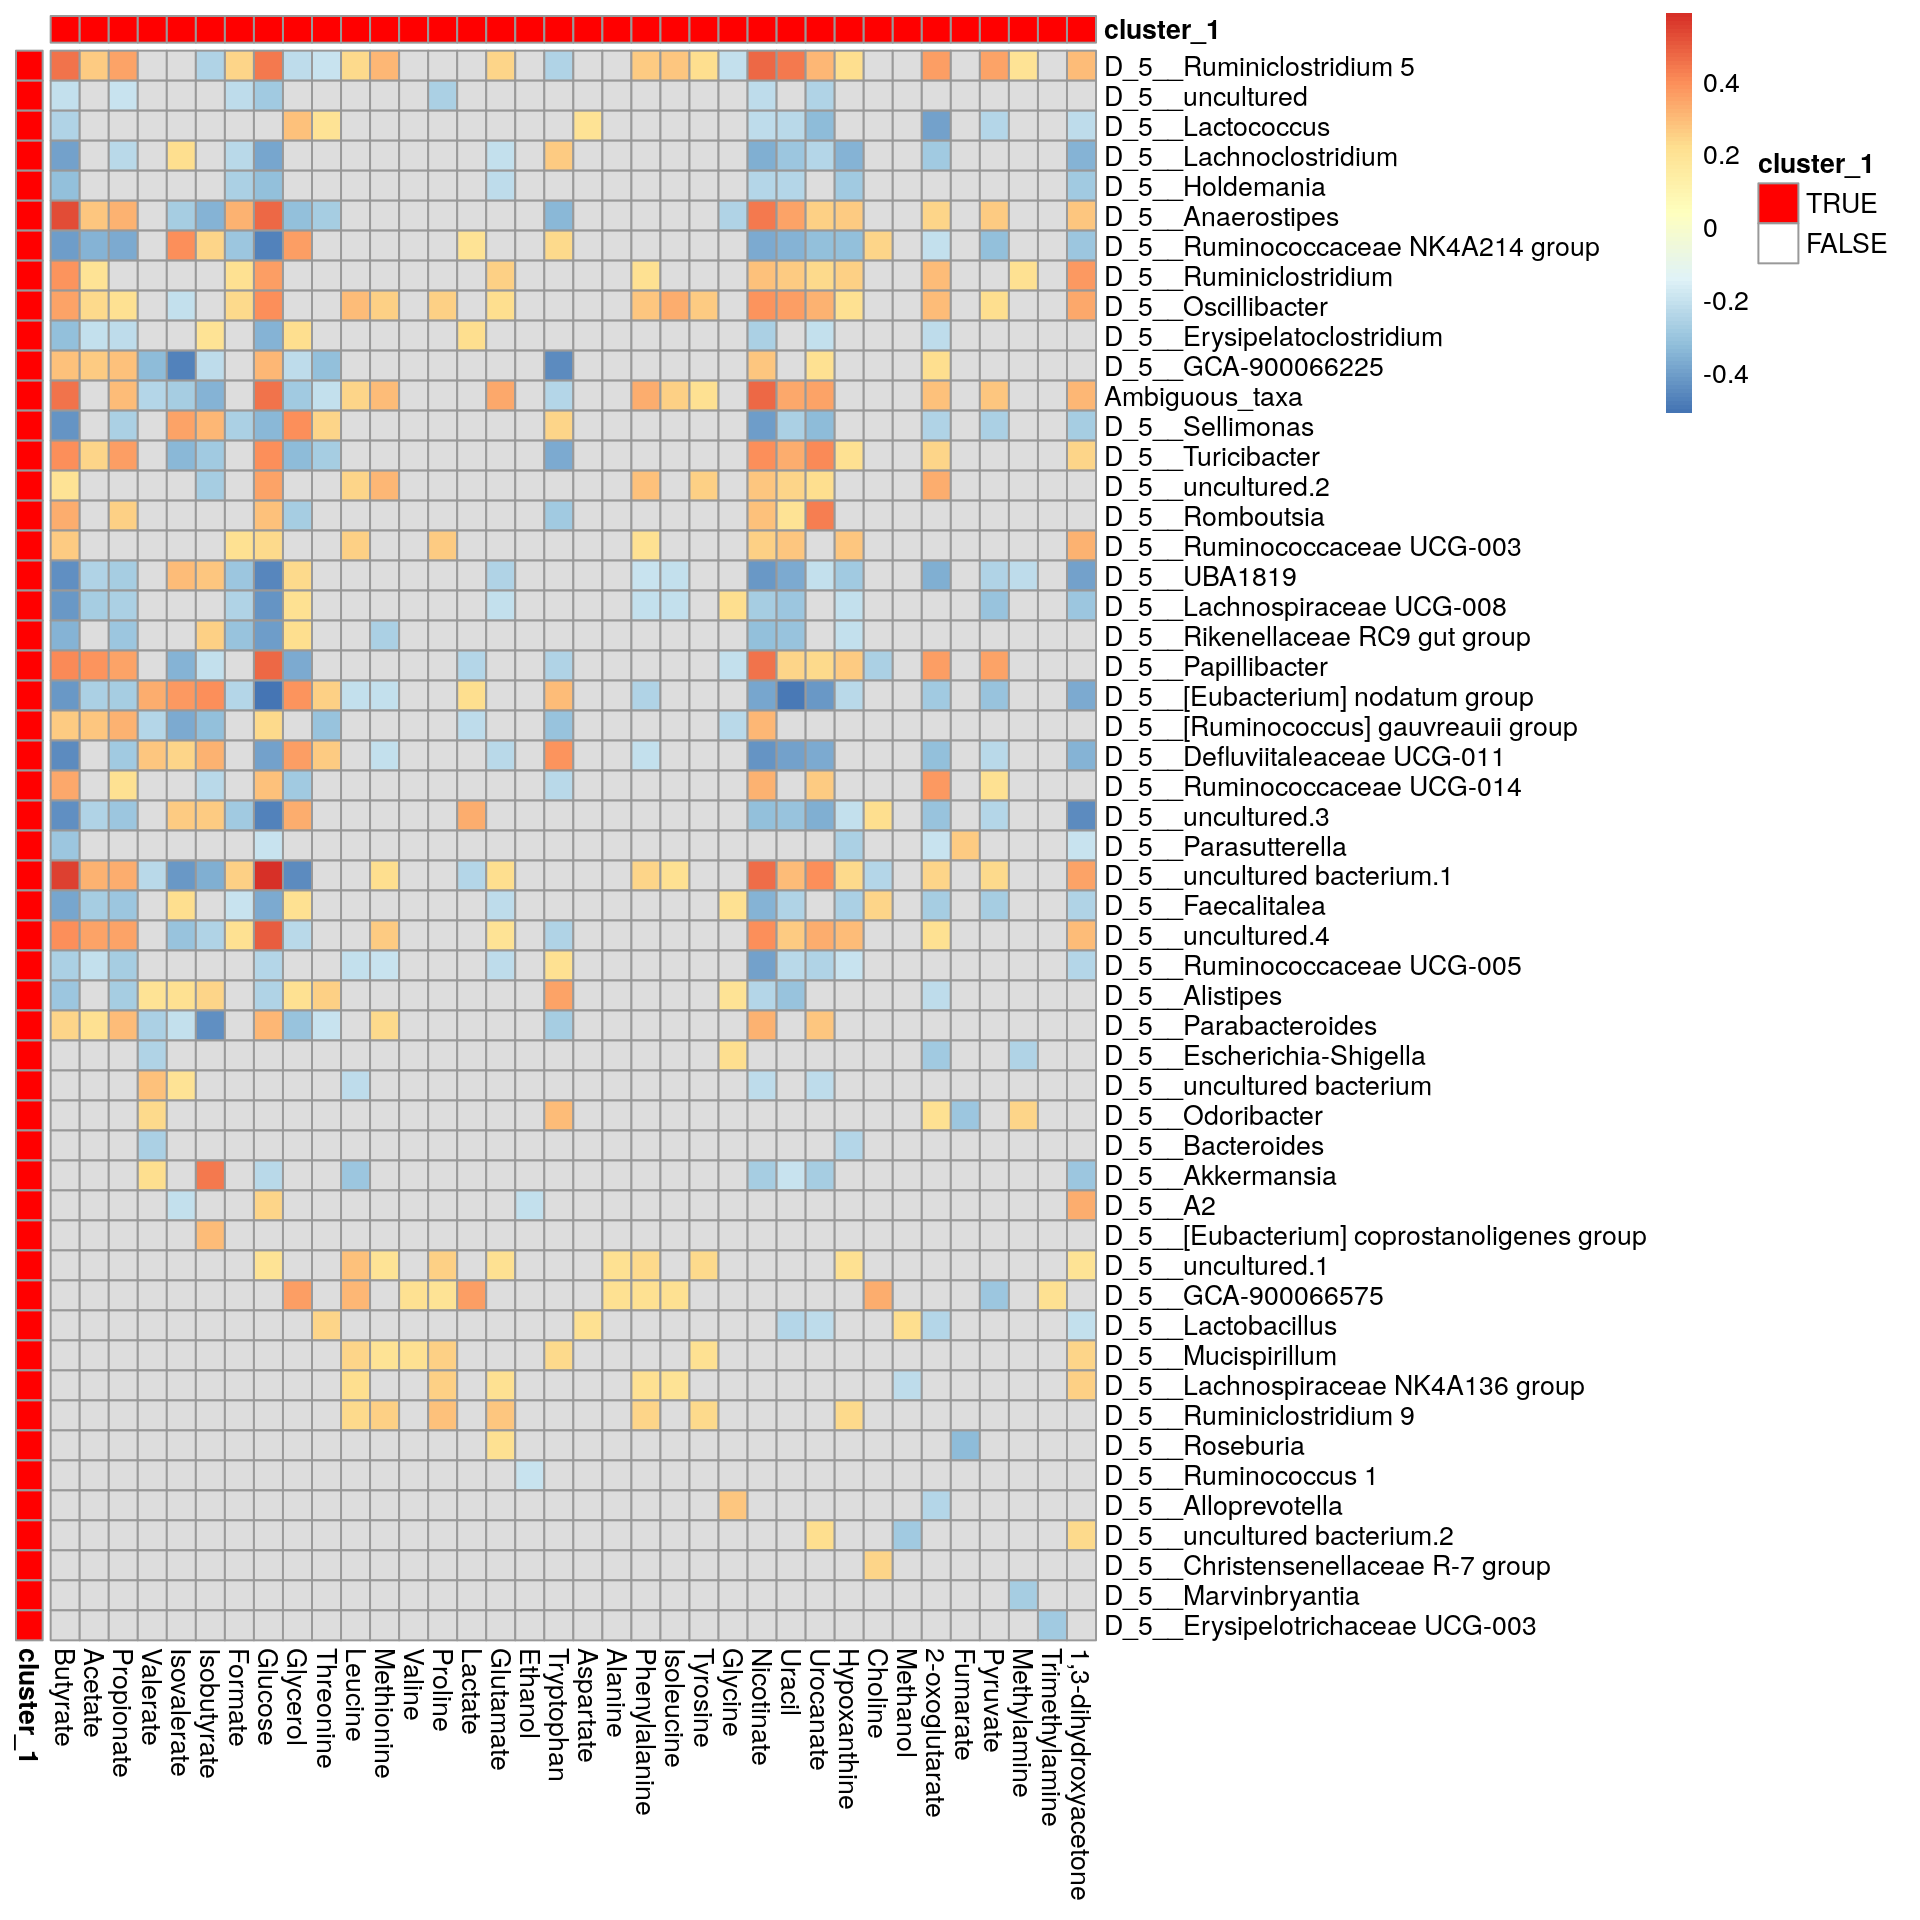
\includegraphics{24_biclustering_files/figure-latex/biclust_8-1.pdf}

\hypertarget{taxa-vs-taxa}{%
\section{Taxa vs taxa}\label{taxa-vs-taxa}}

Third and final example deals with situation where we want to analyze correlation
between taxa. \emph{biclust} is suitable for this.

\begin{Shaded}
\begin{Highlighting}[]
\CommentTok{\# Calculate cross{-}correlation}
\NormalTok{corr }\OtherTok{\textless{}{-}} \FunctionTok{getExperimentCrossCorrelation}\NormalTok{(mae, }\DecValTok{1}\NormalTok{, }\DecValTok{1}\NormalTok{, }
                                      \AttributeTok{abund\_values1 =} \StringTok{"clr"}\NormalTok{, }\AttributeTok{abund\_values2 =} \StringTok{"clr"}\NormalTok{, }
                                      \AttributeTok{mode =} \StringTok{"matrix"}\NormalTok{,}
                                      \AttributeTok{cor\_threshold =} \FloatTok{0.2}\NormalTok{, }\AttributeTok{verbose =}\NormalTok{ F, }\AttributeTok{show\_warning =}\NormalTok{ F)}

\CommentTok{\# Find biclusters}
\NormalTok{bc }\OtherTok{\textless{}{-}} \FunctionTok{biclust}\NormalTok{(corr, }\AttributeTok{method=}\FunctionTok{BCPlaid}\NormalTok{(), }\AttributeTok{fit.model =}\NormalTok{ y }\SpecialCharTok{\textasciitilde{}}\NormalTok{ m,}
              \AttributeTok{background =} \ConstantTok{TRUE}\NormalTok{, }\AttributeTok{shuffle =} \DecValTok{100}\NormalTok{, }\AttributeTok{back.fit =} \DecValTok{0}\NormalTok{, }\AttributeTok{max.layers =} \DecValTok{10}\NormalTok{,}
              \AttributeTok{iter.startup =} \DecValTok{10}\NormalTok{, }\AttributeTok{iter.layer =} \DecValTok{100}\NormalTok{, }\AttributeTok{verbose =} \ConstantTok{FALSE}\NormalTok{)}
\end{Highlighting}
\end{Shaded}

\begin{Shaded}
\begin{Highlighting}[]
\CommentTok{\# Get biclusters}
\NormalTok{bcs }\OtherTok{\textless{}{-}} \FunctionTok{.get\_biclusters\_from\_biclust}\NormalTok{(bc, corr)}

\NormalTok{bicluster\_rows }\OtherTok{\textless{}{-}}\NormalTok{ bcs}\SpecialCharTok{$}\NormalTok{bc\_rows}
\NormalTok{bicluster\_columns }\OtherTok{\textless{}{-}}\NormalTok{ bcs}\SpecialCharTok{$}\NormalTok{bc\_columns}
\end{Highlighting}
\end{Shaded}

\begin{Shaded}
\begin{Highlighting}[]
\CommentTok{\# Create a column that combines information}
\CommentTok{\# If row/column includes in multiple clusters, cluster numbers are separated with "\_\&\_"}
\NormalTok{bicluster\_columns}\SpecialCharTok{$}\NormalTok{clusters }\OtherTok{\textless{}{-}} \FunctionTok{apply}\NormalTok{(bicluster\_columns, }\DecValTok{1}\NormalTok{, }
                                    \ControlFlowTok{function}\NormalTok{(x)\{}\FunctionTok{paste}\NormalTok{(}\FunctionTok{paste}\NormalTok{(}\FunctionTok{which}\NormalTok{(x)), }\AttributeTok{collapse =} \StringTok{"\_\&\_"}\NormalTok{) \})}
\NormalTok{bicluster\_columns }\OtherTok{\textless{}{-}}\NormalTok{ bicluster\_columns[, }\StringTok{"clusters"}\NormalTok{, drop }\OtherTok{=} \ConstantTok{FALSE}\NormalTok{]}

\NormalTok{bicluster\_rows}\SpecialCharTok{$}\NormalTok{clusters }\OtherTok{\textless{}{-}} \FunctionTok{apply}\NormalTok{(bicluster\_rows, }\DecValTok{1}\NormalTok{, }
                                 \ControlFlowTok{function}\NormalTok{(x)\{}\FunctionTok{paste}\NormalTok{(}\FunctionTok{paste}\NormalTok{(}\FunctionTok{which}\NormalTok{(x)), }\AttributeTok{collapse =} \StringTok{"\_\&\_"}\NormalTok{) \})}
\NormalTok{bicluster\_rows }\OtherTok{\textless{}{-}}\NormalTok{ bicluster\_rows[, }\StringTok{"clusters"}\NormalTok{, drop }\OtherTok{=} \ConstantTok{FALSE}\NormalTok{]}
\end{Highlighting}
\end{Shaded}

\begin{Shaded}
\begin{Highlighting}[]
\CommentTok{\# Convert boolean values into factor}
\NormalTok{bicluster\_columns }\OtherTok{\textless{}{-}} \FunctionTok{data.frame}\NormalTok{(}\FunctionTok{apply}\NormalTok{(bicluster\_columns, }\DecValTok{2}\NormalTok{, as.factor))}
\NormalTok{bicluster\_rows }\OtherTok{\textless{}{-}} \FunctionTok{data.frame}\NormalTok{(}\FunctionTok{apply}\NormalTok{(bicluster\_rows, }\DecValTok{2}\NormalTok{, as.factor))}

\FunctionTok{pheatmap}\NormalTok{(corr, }\AttributeTok{cluster\_cols =}\NormalTok{ F, }\AttributeTok{cluster\_rows =}\NormalTok{ F,}
         \AttributeTok{annotation\_col =}\NormalTok{ bicluster\_columns, }
         \AttributeTok{annotation\_row =}\NormalTok{ bicluster\_rows)}
\end{Highlighting}
\end{Shaded}

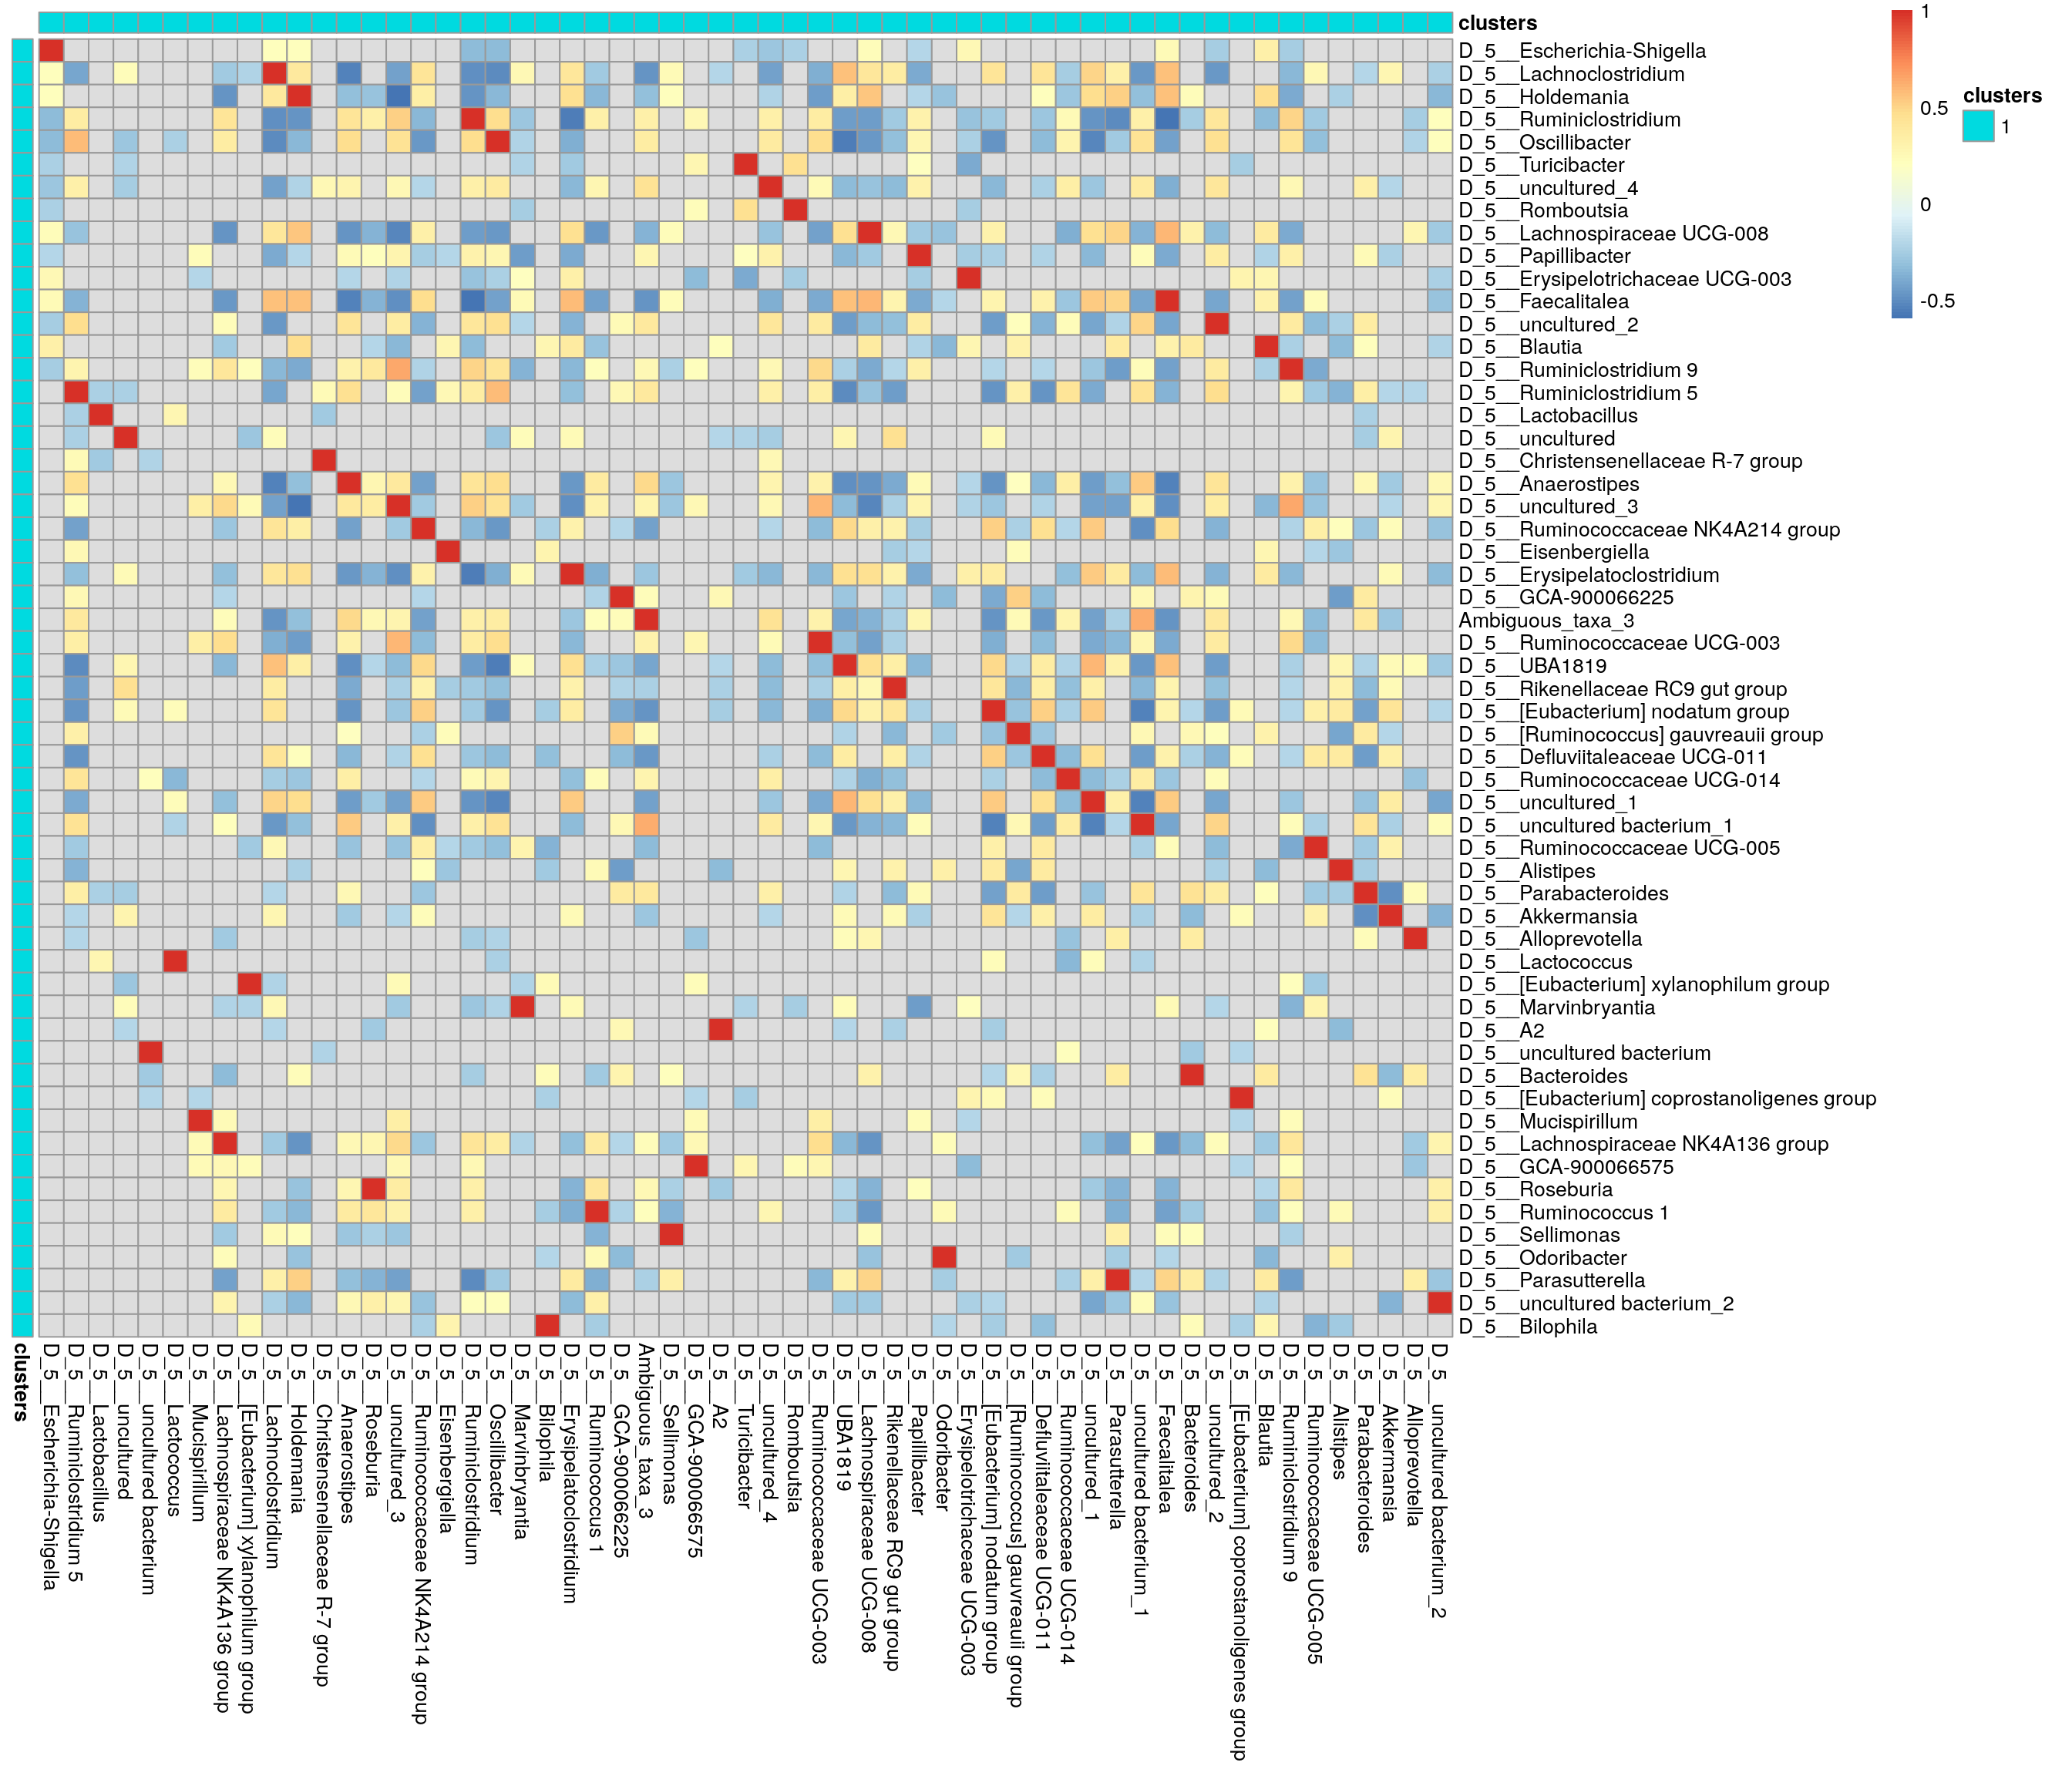
\includegraphics{24_biclustering_files/figure-latex/biclust_12-1.pdf}

\hypertarget{session-info-7}{%
\section*{Session Info}\label{session-info-7}}
\addcontentsline{toc}{section}{Session Info}

View session info

\begin{verbatim}
R version 4.1.2 (2021-11-01)
Platform: x86_64-pc-linux-gnu (64-bit)
Running under: Ubuntu 20.04.3 LTS

Matrix products: default
BLAS/LAPACK: /usr/lib/x86_64-linux-gnu/openblas-pthread/libopenblasp-r0.3.8.so

locale:
 [1] LC_CTYPE=en_US.UTF-8       LC_NUMERIC=C              
 [3] LC_TIME=en_US.UTF-8        LC_COLLATE=en_US.UTF-8    
 [5] LC_MONETARY=en_US.UTF-8    LC_MESSAGES=en_US.UTF-8   
 [7] LC_PAPER=en_US.UTF-8       LC_NAME=C                 
 [9] LC_ADDRESS=C               LC_TELEPHONE=C            
[11] LC_MEASUREMENT=en_US.UTF-8 LC_IDENTIFICATION=C       

attached base packages:
[1] grid      stats4    stats     graphics  grDevices utils     datasets 
[8] methods   base     

other attached packages:
 [1] biclust_2.0.3                  lattice_0.20-45               
 [3] colorspace_2.0-3               MASS_7.3-55                   
 [5] patchwork_1.1.1                ggplot2_3.3.5                 
 [7] pheatmap_1.0.12                cobiclust_0.1.0               
 [9] microbiomeDataSets_1.1.5       mia_1.3.19                    
[11] MultiAssayExperiment_1.20.0    TreeSummarizedExperiment_2.1.4
[13] Biostrings_2.62.0              XVector_0.34.0                
[15] SingleCellExperiment_1.16.0    SummarizedExperiment_1.24.0   
[17] Biobase_2.54.0                 GenomicRanges_1.46.1          
[19] GenomeInfoDb_1.30.1            IRanges_2.28.0                
[21] S4Vectors_0.32.3               BiocGenerics_0.40.0           
[23] MatrixGenerics_1.6.0           matrixStats_0.61.0-9001       
[25] BiocStyle_2.22.0               rebook_1.4.0                  

loaded via a namespace (and not attached):
  [1] AnnotationHub_3.2.2           BiocFileCache_2.2.1          
  [3] plyr_1.8.6                    lazyeval_0.2.2               
  [5] splines_4.1.2                 BiocParallel_1.28.3          
  [7] scater_1.22.0                 digest_0.6.29                
  [9] yulab.utils_0.0.4             htmltools_0.5.2              
 [11] viridis_0.6.2                 fansi_1.0.2                  
 [13] magrittr_2.0.2                memoise_2.0.1                
 [15] ScaledMatrix_1.2.0            cluster_2.1.2                
 [17] DECIPHER_2.22.0               blob_1.2.2                   
 [19] rappdirs_0.3.3                ggrepel_0.9.1                
 [21] xfun_0.30                     dplyr_1.0.8                  
 [23] crayon_1.5.0                  RCurl_1.98-1.6               
 [25] jsonlite_1.8.0                graph_1.72.0                 
 [27] ape_5.6-2                     glue_1.6.2                   
 [29] gtable_0.3.0                  zlibbioc_1.40.0              
 [31] DelayedArray_0.20.0           additivityTests_1.1-4        
 [33] BiocSingular_1.10.0           scales_1.1.1                 
 [35] DBI_1.1.2                     Rcpp_1.0.8.3                 
 [37] viridisLite_0.4.0             xtable_1.8-4                 
 [39] decontam_1.14.0               tidytree_0.3.9               
 [41] bit_4.0.4                     rsvd_1.0.5                   
 [43] httr_1.4.2                    RColorBrewer_1.1-2           
 [45] dir.expiry_1.2.0              modeltools_0.2-23            
 [47] ellipsis_0.3.2                farver_2.1.0                 
 [49] pkgconfig_2.0.3               XML_3.99-0.9                 
 [51] scuttle_1.4.0                 CodeDepends_0.6.5            
 [53] dbplyr_2.1.1                  utf8_1.2.2                   
 [55] labeling_0.4.2                tidyselect_1.1.2             
 [57] rlang_1.0.2                   reshape2_1.4.4               
 [59] later_1.3.0                   AnnotationDbi_1.56.2         
 [61] munsell_0.5.0                 BiocVersion_3.14.0           
 [63] tools_4.1.2                   cachem_1.0.6                 
 [65] cli_3.2.0                     DirichletMultinomial_1.36.0  
 [67] generics_0.1.2                RSQLite_2.2.10               
 [69] ExperimentHub_2.2.1           evaluate_0.15                
 [71] stringr_1.4.0                 fastmap_1.1.0                
 [73] yaml_2.3.5                    knitr_1.37                   
 [75] bit64_4.0.5                   purrr_0.3.4                  
 [77] KEGGREST_1.34.0               nlme_3.1-155                 
 [79] sparseMatrixStats_1.6.0       mime_0.12                    
 [81] flexclust_1.4-0               compiler_4.1.2               
 [83] beeswarm_0.4.0                filelock_1.0.2               
 [85] curl_4.3.2                    png_0.1-7                    
 [87] interactiveDisplayBase_1.32.0 treeio_1.18.1                
 [89] tibble_3.1.6                  stringi_1.7.6                
 [91] highr_0.9                     Matrix_1.4-0                 
 [93] vegan_2.5-7                   permute_0.9-7                
 [95] vctrs_0.3.8                   pillar_1.7.0                 
 [97] lifecycle_1.0.1               BiocManager_1.30.16          
 [99] BiocNeighbors_1.12.0          bitops_1.0-7                 
[101] irlba_2.3.5                   httpuv_1.6.5                 
[103] R6_2.5.1                      bookdown_0.25                
[105] promises_1.2.0.1              gridExtra_2.3                
[107] vipor_0.4.5                   codetools_0.2-18             
[109] assertthat_0.2.1              withr_2.5.0                  
[111] GenomeInfoDbData_1.2.7        mgcv_1.8-39                  
[113] parallel_4.1.2                beachmat_2.10.0              
[115] class_7.3-20                  tidyr_1.2.0                  
[117] rmarkdown_2.13                DelayedMatrixStats_1.16.0    
[119] shiny_1.7.1                   ggbeeswarm_0.6.0             
\end{verbatim}

\hypertarget{differential-abundance}{%
\chapter{Differential abundance}\label{differential-abundance}}

\hypertarget{differential-abundance-analysis}{%
\section{Differential abundance analysis}\label{differential-abundance-analysis}}

This section provides an overview and examples of \emph{differential
abundance analysis (DAA)} based on one of the \href{https://microbiome.github.io/mia/reference/mia-datasets.html}{openly available
datasets}
in mia to illustrate how to perform differential abundance analysis
(DAA). DAA identifies differences in the abundances of individual
taxonomic groups between two or more groups (e.g.~treatment vs
control). This can be performed at any phylogenetic level.

We perform DAA to identify biomarkers and/or gain understanding of a
complex system by looking at its isolated components. For example,
identifying that a bacterial taxon is different between e.g.~a patient
group with disease \emph{X} vs a healthy control group might lead to
important insights into the pathophysiology. Changes in the microbiota
might be causal or a consequence of the disease. Either way, it can
help to understand the system as a whole. Be aware that this approach
has also been criticized recently \citep{quinnCritiqueDifferentialAbundance2021}.

\hypertarget{examples-and-tools}{%
\subsection{Examples and tools}\label{examples-and-tools}}

There are many tools to perform DAA. The most popular tools, without going into
evaluating whether or not they perform well for this task, are:\\
- \href{https://bioconductor.org/packages/release/bioc/html/ALDEx2.html}{ALDEx2}\\
- \href{https://bioconductor.org/packages/release/bioc/html/ANCOMBC.html}{ANCOM-BC}\\
- \href{https://cran.r-project.org/web/packages/corncob/index.html}{corncob}\\
- \href{https://bioconductor.org/packages/release/bioc/html/DESeq2.html}{DESeq2}\\
- \href{https://bioconductor.org/packages/release/bioc/html/edgeR.html}{edgeR}\\
- \href{https://bioconductor.org/packages/release/bioc/html/lefser.html}{LEFse}\\
- \href{https://www.bioconductor.org/packages/release/bioc/html/Maaslin2.html}{MaAsLin2}\\
- \href{https://www.bioconductor.org/packages/release/bioc/html/metagenomeSeq.html}{metagenomeSeq}\\
- \href{https://bioconductor.org/packages/release/bioc/html/limma.html}{limma voom}\\
- \href{https://www.rdocumentation.org/packages/stats/versions/3.6.2/topics/t.test}{t-test}\\
- \href{https://www.rdocumentation.org/packages/stats/versions/3.6.2/topics/wilcox.test}{Wilcoxon test}

We recommend to have a look at \citet{nearingMicrobiomeDifferentialAbundance2021} who compared all these listed methods across 38
different datasets. Because different methods have different approaches
(parametric vs non-parametric, different normalization techiniques etc.) to
perform the same task (test differential abundance), results can differ between
methods. Unfortunately, as \citet{nearingMicrobiomeDifferentialAbundance2021} point out, they differ disturbingly
much. Therefore, it is highly recommended to pick several methods to get an
idea about how robust and potentially reproducible your findings are depending
on the method. In this section we demonstrate 3 methods that can be recommended
based on this recent review (ANCOM-BC, ALDEx2 and Maaslin2) and we will compare
the results between them.
Note that the purpose of this section is to show how to perform DAA in R, not
how to correctly do causal inference. E.g. there might be confounding factors
that might drive (the absence of) differences between the shown groups that we
ignore for simplicity. However, we will show how you could include covariates
in those models. Furthermore, we picked a dataset that merely has
microbial abundances in a TSE object as well as a grouping variable in the
sample data. We simplify the analysis by only including 2 of the 3 groups.

\begin{Shaded}
\begin{Highlighting}[]
\FunctionTok{library}\NormalTok{(mia)}
\FunctionTok{library}\NormalTok{(patchwork)}
\FunctionTok{library}\NormalTok{(tidySummarizedExperiment)}
\FunctionTok{library}\NormalTok{(ANCOMBC)}
\FunctionTok{library}\NormalTok{(ALDEx2)}
\FunctionTok{library}\NormalTok{(Maaslin2)}
\FunctionTok{library}\NormalTok{(knitr)}
\FunctionTok{library}\NormalTok{(tidyverse)}

\CommentTok{\# we use the dmn\_se dataset and restrict it to }
\CommentTok{\# obese vs lean for easy illustration}
\FunctionTok{data}\NormalTok{(dmn\_se)}
\NormalTok{se }\OtherTok{\textless{}{-}}\NormalTok{ dmn\_se}
\NormalTok{se }\OtherTok{\textless{}{-}}\NormalTok{ se[ ,}\FunctionTok{colData}\NormalTok{(se)}\SpecialCharTok{$}\NormalTok{pheno }\SpecialCharTok{!=} \StringTok{"Overwt"}\NormalTok{]}
\FunctionTok{colData}\NormalTok{(se)}\SpecialCharTok{$}\NormalTok{pheno }\OtherTok{\textless{}{-}} \FunctionTok{fct\_drop}\NormalTok{(}\FunctionTok{colData}\NormalTok{(se)}\SpecialCharTok{$}\NormalTok{pheno, }\StringTok{"Overwt"}\NormalTok{)}
\CommentTok{\# how many observations do we have per group?}
\FunctionTok{count}\NormalTok{(}\FunctionTok{as.data.frame}\NormalTok{(}\FunctionTok{colData}\NormalTok{(se)), pheno) }\SpecialCharTok{\%\textgreater{}\%} \FunctionTok{kable}\NormalTok{()}
\end{Highlighting}
\end{Shaded}

\begin{tabular}{l|r}
\hline
pheno & n\\
\hline
Lean & 61\\
\hline
Obese & 193\\
\hline
\end{tabular}

\begin{Shaded}
\begin{Highlighting}[]
\CommentTok{\# set a seed because some tools can randomly vary and then produce }
\CommentTok{\# different results:}
\FunctionTok{set.seed}\NormalTok{(}\DecValTok{1}\NormalTok{)}
\end{Highlighting}
\end{Shaded}

\hypertarget{prevalence-filtering}{%
\subsection{Prevalence Filtering}\label{prevalence-filtering}}

Before we jump to our analyses, we may want to perform prevalence filtering.
\citet{nearingMicrobiomeDifferentialAbundance2021} found that applying a 10\% threshold for the prevalence of
the taxa generally resulted in more robust results. Some tools have builtin
arguments for that. By applying the threshold to our input data, we can make
sure it is applied for all tools. Below we show how to do this in \texttt{mia}:

\begin{Shaded}
\begin{Highlighting}[]
\NormalTok{se }\OtherTok{\textless{}{-}} \FunctionTok{subsetByPrevalentTaxa}\NormalTok{(se, }\AttributeTok{detection =} \DecValTok{0}\NormalTok{, }\AttributeTok{prevalence =} \FloatTok{0.1}\NormalTok{)}
\end{Highlighting}
\end{Shaded}

\hypertarget{aldex2}{%
\subsection{ALDEx2}\label{aldex2}}

In this section, we will show how to perform a simple ALDEx2 analysis. If you
would choose to pick a single method, this method could be recommended to use.
According to the developers experience, it tends to identify the common
features identified by other methods. This statement is in line with a recent
independent evaluation by \citet{nearingMicrobiomeDifferentialAbundance2021}. Please also have a look at
the more extensive \href{https://bioconductor.org/packages/release/bioc/vignettes/ALDEx2/inst/doc/ALDEx2_vignette.html}{vignette}
that covers this flexible tool in more depth. ALDEx2 estimates technical
variation within each sample per taxon by utilizing the Dirichlet distribution.
It furthermore applies the centered-log-ratio transformation (or closely
related log-ratio transforms). Depending on the experimental setup, it will
perform a two sample Welch's T-test and Wilcoxon-test or a one-way ANOVA and
Kruskal-Wallis-test. For more complex study designs, there is a possibility to
utilize the \texttt{glm} functionality within ALDEx2. The Benjamini-Hochberg procedure
is applied in any case to correct for multiple testing. Below we show a simple
example that illustrates the workflow.

\begin{Shaded}
\begin{Highlighting}[]
\CommentTok{\# Generate Monte Carlo samples of the Dirichlet distribution for each sample.}
\CommentTok{\# Convert each instance using the centred log{-}ratio transform.}
\CommentTok{\# This is the input for all further analyses.}
\NormalTok{x }\OtherTok{\textless{}{-}} \FunctionTok{aldex.clr}\NormalTok{(}
  \AttributeTok{reads =} \FunctionTok{assay}\NormalTok{(se),}
  \AttributeTok{conds =} \FunctionTok{colData}\NormalTok{(se)}\SpecialCharTok{$}\NormalTok{pheno, }
  \CommentTok{\# 128 recommened for ttest, 1000 for rigorous effect size calculation}
  \AttributeTok{mc.samples =} \DecValTok{128}\NormalTok{, }
  \AttributeTok{denom =} \StringTok{"all"}\NormalTok{,}
  \AttributeTok{verbose =} \ConstantTok{FALSE}
\NormalTok{)}
\CommentTok{\# calculates expected values of the Welch\textquotesingle{}s t{-}test and Wilcoxon rank test on}
\CommentTok{\# the data returned by aldex.clr}
\NormalTok{x\_tt }\OtherTok{\textless{}{-}} \FunctionTok{aldex.ttest}\NormalTok{(}
\NormalTok{  x, }
  \AttributeTok{paired.test =} \ConstantTok{FALSE}\NormalTok{, }
  \AttributeTok{verbose =} \ConstantTok{FALSE}\NormalTok{)}
\CommentTok{\# determines the median clr abundance of the feature in all samples and in}
\CommentTok{\# groups, the median difference between the two groups, the median variation}
\CommentTok{\# within each group and the effect size, which is the median of the ratio}
\CommentTok{\# of the between group difference and the larger of the variance within groups}
\NormalTok{x\_effect }\OtherTok{\textless{}{-}} \FunctionTok{aldex.effect}\NormalTok{(x, }\AttributeTok{CI =} \ConstantTok{TRUE}\NormalTok{, }\AttributeTok{verbose =} \ConstantTok{FALSE}\NormalTok{)}
\CommentTok{\# combine all outputs }
\NormalTok{aldex\_out }\OtherTok{\textless{}{-}} \FunctionTok{data.frame}\NormalTok{(x\_tt, x\_effect)}
\end{Highlighting}
\end{Shaded}

Now, we can create a so called Bland-Altman or MA plot (left). It shows the
association between the relative abundance and the magnitude of the difference
per sample. Next to that, we can also create a plot that shows the dispersion
on the x-axis instead of log-ratio abundance. Red dots represent genera that are
differentially abundant (\(q \leq 0.1\)) between the 2 groups. Black points are
rare taxa and grey ones are abundant taxa.

\begin{Shaded}
\begin{Highlighting}[]
\FunctionTok{par}\NormalTok{(}\AttributeTok{mfrow =} \FunctionTok{c}\NormalTok{(}\DecValTok{1}\NormalTok{, }\DecValTok{2}\NormalTok{))}
  \FunctionTok{aldex.plot}\NormalTok{(}
\NormalTok{    aldex\_out, }
    \AttributeTok{type =} \StringTok{"MA"}\NormalTok{, }
    \AttributeTok{test =} \StringTok{"welch"}\NormalTok{, }
    \AttributeTok{xlab =} \StringTok{"Log{-}ratio abundance"}\NormalTok{,}
    \AttributeTok{ylab =} \StringTok{"Difference"}\NormalTok{,}
    \AttributeTok{cutoff =} \FloatTok{0.05}
\NormalTok{  )}
  \FunctionTok{aldex.plot}\NormalTok{(}
\NormalTok{    aldex\_out, }
    \AttributeTok{type =} \StringTok{"MW"}\NormalTok{, }
    \AttributeTok{test =} \StringTok{"welch"}\NormalTok{,}
    \AttributeTok{xlab =} \StringTok{"Dispersion"}\NormalTok{,}
    \AttributeTok{ylab =} \StringTok{"Difference"}\NormalTok{,}
    \AttributeTok{cutoff =} \FloatTok{0.05}
\NormalTok{  )}
\end{Highlighting}
\end{Shaded}

\includegraphics{30_differential_abundance_files/figure-latex/unnamed-chunk-3-1.pdf}

The evaluation as differential abundant in above plots is based on the
corrected pvalue. According to the ALDEx2 developers, the safest approach is to
identify those features where the 95\% CI of the
effect size does not cross 0. As we can see in below table, this is not the
case for any of the identified
genera (see overlap column, which indicates the proportion of overlap). Also,
the authors recommend an effect
size cutoff of 1 rather than only interpreting the pvalue. Again, this is not
the case for any feature.

\begin{Shaded}
\begin{Highlighting}[]
\FunctionTok{rownames\_to\_column}\NormalTok{(aldex\_out, }\StringTok{"genus"}\NormalTok{) }\SpecialCharTok{\%\textgreater{}\%}
  \FunctionTok{filter}\NormalTok{(wi.eBH }\SpecialCharTok{\textless{}=} \FloatTok{0.05}\NormalTok{)  }\SpecialCharTok{\%\textgreater{}\%} \CommentTok{\# here we chose the wilcoxon output rather than tt}
  \FunctionTok{select}\NormalTok{(genus, we.eBH, wi.eBH, effect, overlap) }\SpecialCharTok{\%\textgreater{}\%}
  \FunctionTok{kable}\NormalTok{()}
\end{Highlighting}
\end{Shaded}

\begin{tabular}{l|r|r|r|r}
\hline
genus & we.eBH & wi.eBH & effect & overlap\\
\hline
Alistipes & 0.0009 & 0.0001 & -0.3823 & 0.2979\\
\hline
Barnesiella & 0.0442 & 0.0066 & -0.3229 & 0.3489\\
\hline
Catenibacterium & 0.0266 & 0.0330 & 0.2713 & 0.3718\\
\hline
Lactobacillus & 0.0282 & 0.0183 & 0.2983 & 0.3537\\
\hline
Megasphaera & 0.0000 & 0.0001 & 0.5249 & 0.2758\\
\hline
Oscillibacter & 0.0004 & 0.0014 & -0.3681 & 0.3291\\
\hline
Parabacteroides & 0.0541 & 0.0133 & -0.2832 & 0.3509\\
\hline
Phascolarctobacterium & 0.0238 & 0.0077 & -0.3491 & 0.3404\\
\hline
Uknown & 0.0786 & 0.0439 & -0.2474 & 0.3852\\
\hline
\end{tabular}

\hypertarget{ancom-bc}{%
\subsection{ANCOM-BC}\label{ancom-bc}}

The analysis of composition of microbiomes with bias correction
(ANCOM-BC) \citep{linAnalysisCompositionsMicrobiomes2020}
is a recently developed method for differential abundance testing. It is based
on an
earlier published approach \citep{mandalAnalysisCompositionMicrobiomes2015}.
The previous version of ANCOM was among the methods that produced the
most consistent results and is probably a conservative approach
\citep{nearingMicrobiomeDifferentialAbundance2021}.
However, the new ANCOM-BC method operates quite differently compared to the
former ANCOM method.

As the only method, ANCOM-BC incorporates the so called \emph{sampling fraction}
into the model. The latter term could be empirically estimated by the ratio of
the library size to the microbial load. According to the authors, variations in
this sampling fraction would bias differential abundance analyses if ignored.
Furthermore, this method provides p-values, and confidence intervals for each
taxon. It also controls the FDR and it is computationally simple to implement.

As we will see below, to obtain results, all that is needed is to pass
a phyloseq object to the \texttt{ancombc()} function. Therefore, below we first
convert our \texttt{se} object to a \texttt{phyloseq} object. Then, we specify the formula.
In this formula, other covariates could potentially be included to adjust for
confounding. We show this further below.
Please check the \href{https://rdrr.io/github/FrederickHuangLin/ANCOMBC/man/ancombc.html}{function documentation}
to learn about the additional arguments that we specify below.

\begin{Shaded}
\begin{Highlighting}[]
\CommentTok{\# currently, ancombc requires the phyloseq format, but we can easily convert:}
\NormalTok{pseq }\OtherTok{\textless{}{-}} \FunctionTok{makePhyloseqFromTreeSummarizedExperiment}\NormalTok{(se)}

\CommentTok{\# perform the analysis }
\NormalTok{out }\OtherTok{=} \FunctionTok{ancombc}\NormalTok{(}
  \AttributeTok{phyloseq =}\NormalTok{ pseq, }
  \AttributeTok{formula =} \StringTok{"pheno"}\NormalTok{, }
  \AttributeTok{p\_adj\_method =} \StringTok{"fdr"}\NormalTok{, }
  \AttributeTok{zero\_cut =} \DecValTok{1}\NormalTok{, }\CommentTok{\# no prev filtering necessary anymore }
  \AttributeTok{lib\_cut =} \DecValTok{0}\NormalTok{, }
  \AttributeTok{group =} \StringTok{"pheno"}\NormalTok{, }
  \AttributeTok{struc\_zero =} \ConstantTok{TRUE}\NormalTok{, }
  \AttributeTok{neg\_lb =} \ConstantTok{TRUE}\NormalTok{, }
  \AttributeTok{tol =} \FloatTok{1e{-}5}\NormalTok{, }
  \AttributeTok{max\_iter =} \DecValTok{100}\NormalTok{, }
  \AttributeTok{conserve =} \ConstantTok{TRUE}\NormalTok{, }
  \AttributeTok{alpha =} \FloatTok{0.05}\NormalTok{, }
  \AttributeTok{global =} \ConstantTok{TRUE}
\NormalTok{)}
\CommentTok{\# store the results in res }
\NormalTok{res }\OtherTok{\textless{}{-}}\NormalTok{ out}\SpecialCharTok{$}\NormalTok{res}
\end{Highlighting}
\end{Shaded}

The object \texttt{out} contains all model output. Again, see the
\href{https://rdrr.io/github/FrederickHuangLin/ANCOMBC/man/ancombc.html}{documentation of the function}
under \textbf{Value} for an explanation of all the output objects. Our question
whether taxa are differentially abundant can be answered by looking at the
\texttt{res} object, which now contains dataframes with the coefficients,
standard errors, p-values and q-values. Conveniently, there is a dataframe
\texttt{diff\_abn}. Here, for each taxon it is indicated whether it is differentially
abundant between the groups. Below we show the first 6 entries of this
dataframe:

\begin{Shaded}
\begin{Highlighting}[]
\FunctionTok{kable}\NormalTok{(}\FunctionTok{head}\NormalTok{(res}\SpecialCharTok{$}\NormalTok{diff\_abn))}
\end{Highlighting}
\end{Shaded}

\begin{tabular}{l|l}
\hline
  & phenoObese\\
\hline
Acetanaerobacterium & TRUE\\
\hline
Acetivibrio & FALSE\\
\hline
Acidaminococcus & TRUE\\
\hline
Akkermansia & FALSE\\
\hline
Alistipes & TRUE\\
\hline
Allisonella & FALSE\\
\hline
\end{tabular}

\hypertarget{maaslin2}{%
\subsection{MaAsLin2}\label{maaslin2}}

Lastly, we will illustrate how to use MaAsLin2, which is the next generation of
MaAsLin. As it is based on generalized linear models, it is flexible for different study designs and covariate
structures. The official package tutorial can be found \href{https://github.com/biobakery/biobakery/wiki/maaslin2}{here}.

\begin{Shaded}
\begin{Highlighting}[]
\CommentTok{\# maaslin expects features as columns and samples as rows }
\CommentTok{\# for both the asv/otu table as well as meta data }
\NormalTok{asv }\OtherTok{\textless{}{-}} \FunctionTok{t}\NormalTok{(}\FunctionTok{assay}\NormalTok{(se))}
\NormalTok{meta\_data }\OtherTok{\textless{}{-}} \FunctionTok{data.frame}\NormalTok{(}\FunctionTok{colData}\NormalTok{(se))}
\CommentTok{\# you can specifiy different GLMs/normalizations/transforms. We used similar}
\CommentTok{\# settings as in Nearing et al. (2021) here:}
\NormalTok{fit\_data }\OtherTok{\textless{}{-}} \FunctionTok{Maaslin2}\NormalTok{(}
\NormalTok{  asv,}
\NormalTok{  meta\_data,}
  \AttributeTok{output =} \StringTok{"DAA example"}\NormalTok{,}
  \AttributeTok{transform =} \StringTok{"AST"}\NormalTok{,}
  \AttributeTok{fixed\_effects =} \StringTok{"pheno"}\NormalTok{,}
  \CommentTok{\# random\_effects = c(...), \# you can also fit MLM by specifying random effects}
  \CommentTok{\# specifying a ref is especially important if you have more than 2 levels}
  \AttributeTok{reference =} \StringTok{"pheno,Lean"}\NormalTok{,  }
  \AttributeTok{normalization =} \StringTok{"TSS"}\NormalTok{,}
  \AttributeTok{standardize =} \ConstantTok{FALSE}\NormalTok{,}
  \AttributeTok{min\_prevalence =} \DecValTok{0} \CommentTok{\# prev filterin already done}
\NormalTok{)}
\end{Highlighting}
\end{Shaded}

\begin{Shaded}
\begin{Highlighting}[]
\CommentTok{\# which genera are identified as differentially abundant? (leave out "head" to}
\CommentTok{\# see all)}
\FunctionTok{kable}\NormalTok{(}\FunctionTok{head}\NormalTok{(}\FunctionTok{filter}\NormalTok{(fit\_data}\SpecialCharTok{$}\NormalTok{results, qval }\SpecialCharTok{\textless{}=} \FloatTok{0.05}\NormalTok{)))}
\end{Highlighting}
\end{Shaded}

\begin{tabular}{l|l|l|r|r|r|l|r|r|r}
\hline
feature & metadata & value & coef & stderr & pval & name & qval & N & N.not.zero\\
\hline
Megasphaera & pheno & Obese & 0.0489 & 0.0093 & 0 & phenoObese & 0e+00 & 254 & 78\\
\hline
Barnesiella & pheno & Obese & -0.0297 & 0.0068 & 0 & phenoObese & 2e-04 & 254 & 111\\
\hline
Parabacteroides & pheno & Obese & -0.0219 & 0.0050 & 0 & phenoObese & 2e-04 & 254 & 163\\
\hline
Phascolarctobacterium & pheno & Obese & -0.0325 & 0.0072 & 0 & phenoObese & 2e-04 & 254 & 99\\
\hline
Alistipes & pheno & Obese & -0.0523 & 0.0123 & 0 & phenoObese & 3e-04 & 254 & 227\\
\hline
Desulfovibrio & pheno & Obese & -0.0134 & 0.0032 & 0 & phenoObese & 3e-04 & 254 & 72\\
\hline
\end{tabular}

\begin{Shaded}
\begin{Highlighting}[]
\CommentTok{\# A folder will be created that is called like the above specified output.}
\CommentTok{\# It contains also figures to visualize the difference between genera }
\CommentTok{\# for the significant ones.}
\end{Highlighting}
\end{Shaded}

\hypertarget{comparison-of-the-methods}{%
\subsection{Comparison of the methods}\label{comparison-of-the-methods}}

When we compare the methods in the context of a research question, we could
look at e.g.~at whether they agree based on the applied decision criterion
(e.g.~adjusted p value \textless{} 0.05). That is what we illustrate here. First we will
look at how many taxa were identified by each method to begin with. In the next
step we will look at the intersection of identified taxa. To achieve that, we
first create a dataframe that summarises the decision criterion for each method
and shows a score from 0 to 3 indicating how many methods agreed on a particular
taxon.

\begin{Shaded}
\begin{Highlighting}[]
\NormalTok{summ }\OtherTok{\textless{}{-}} \FunctionTok{full\_join}\NormalTok{(}
    \FunctionTok{rownames\_to\_column}\NormalTok{(aldex\_out, }\StringTok{"genus"}\NormalTok{) }\SpecialCharTok{\%\textgreater{}\%}
      \FunctionTok{select}\NormalTok{(genus, }\AttributeTok{aldex2 =}\NormalTok{ wi.eBH),}
    \FunctionTok{rownames\_to\_column}\NormalTok{(out}\SpecialCharTok{$}\NormalTok{res}\SpecialCharTok{$}\NormalTok{diff\_abn, }\StringTok{"genus"}\NormalTok{) }\SpecialCharTok{\%\textgreater{}\%}
      \FunctionTok{select}\NormalTok{(genus, }\AttributeTok{ancombc =}\NormalTok{ phenoObese),}
    \AttributeTok{by =} \StringTok{"genus"}\NormalTok{) }\SpecialCharTok{\%\textgreater{}\%}
  \FunctionTok{full\_join}\NormalTok{(}
    \FunctionTok{select}\NormalTok{(fit\_data}\SpecialCharTok{$}\NormalTok{results, }\AttributeTok{genus =}\NormalTok{ feature, }\AttributeTok{maaslin2 =}\NormalTok{ qval), }
    \AttributeTok{by =} \StringTok{"genus"}\NormalTok{) }\SpecialCharTok{\%\textgreater{}\%}
  \FunctionTok{mutate}\NormalTok{(}
    \FunctionTok{across}\NormalTok{(}\FunctionTok{c}\NormalTok{(aldex2, maaslin2), }\SpecialCharTok{\textasciitilde{}}\NormalTok{ .x }\SpecialCharTok{\textless{}=} \FloatTok{0.05}\NormalTok{),}
    \CommentTok{\# the following line would be necessary without prevalence filtering }
    \CommentTok{\# as some methods output NA}
    \CommentTok{\#across({-}genus, function(x) ifelse(is.na(x), FALSE, x)),}
    \AttributeTok{score =} \FunctionTok{rowSums}\NormalTok{(}\FunctionTok{across}\NormalTok{(}\FunctionTok{c}\NormalTok{(aldex2, ancombc, maaslin2)))}
\NormalTok{  )}

\CommentTok{\# This is how it looks like:}
\FunctionTok{kable}\NormalTok{(}\FunctionTok{head}\NormalTok{(summ))}
\end{Highlighting}
\end{Shaded}

\begin{tabular}{l|l|l|l|r}
\hline
genus & aldex2 & ancombc & maaslin2 & score\\
\hline
Acetanaerobacterium & FALSE & TRUE & TRUE & 2\\
\hline
Acetivibrio & FALSE & FALSE & FALSE & 0\\
\hline
Acidaminococcus & FALSE & TRUE & TRUE & 2\\
\hline
Akkermansia & FALSE & FALSE & FALSE & 0\\
\hline
Alistipes & TRUE & TRUE & TRUE & 3\\
\hline
Allisonella & FALSE & FALSE & FALSE & 0\\
\hline
\end{tabular}

Now we can answer our questions:

\begin{Shaded}
\begin{Highlighting}[]
\CommentTok{\# how many genera were identified by each method?}
\FunctionTok{summarise}\NormalTok{(summ, }\FunctionTok{across}\NormalTok{(}\FunctionTok{where}\NormalTok{(is.logical), sum)) }\SpecialCharTok{\%\textgreater{}\%}
  \FunctionTok{kable}\NormalTok{()}
\end{Highlighting}
\end{Shaded}

\begin{tabular}{r|r|r}
\hline
aldex2 & ancombc & maaslin2\\
\hline
9 & 22 & 16\\
\hline
\end{tabular}

\begin{Shaded}
\begin{Highlighting}[]
\CommentTok{\# which genera are identified by all methods?}
\FunctionTok{filter}\NormalTok{(summ, score }\SpecialCharTok{==} \DecValTok{3}\NormalTok{) }\SpecialCharTok{\%\textgreater{}\%} \FunctionTok{kable}\NormalTok{()}
\end{Highlighting}
\end{Shaded}

\begin{tabular}{l|l|l|l|r}
\hline
genus & aldex2 & ancombc & maaslin2 & score\\
\hline
Alistipes & TRUE & TRUE & TRUE & 3\\
\hline
Barnesiella & TRUE & TRUE & TRUE & 3\\
\hline
Catenibacterium & TRUE & TRUE & TRUE & 3\\
\hline
Lactobacillus & TRUE & TRUE & TRUE & 3\\
\hline
Megasphaera & TRUE & TRUE & TRUE & 3\\
\hline
Oscillibacter & TRUE & TRUE & TRUE & 3\\
\hline
Parabacteroides & TRUE & TRUE & TRUE & 3\\
\hline
Phascolarctobacterium & TRUE & TRUE & TRUE & 3\\
\hline
\end{tabular}

We see that each method identified at least 9 genera as differentially
abundant. Eight of those that were identified by ALDEx2,
were also identified by both of the other methods. We could plot the data for
any method or for those taxa that were identified by all methods:

\begin{Shaded}
\begin{Highlighting}[]
\NormalTok{plot\_data }\OtherTok{\textless{}{-}} \FunctionTok{data.frame}\NormalTok{(}\FunctionTok{t}\NormalTok{(}\FunctionTok{assay}\NormalTok{(se)))}
\NormalTok{plot\_data}\SpecialCharTok{$}\NormalTok{pheno }\OtherTok{\textless{}{-}} \FunctionTok{colData}\NormalTok{(se)}\SpecialCharTok{$}\NormalTok{pheno}
\CommentTok{\# create a plot for each genus where the score is indicated in the title}
\NormalTok{plots }\OtherTok{\textless{}{-}} \FunctionTok{pmap}\NormalTok{(}\FunctionTok{select}\NormalTok{(summ, genus, score), }\ControlFlowTok{function}\NormalTok{(genus, score) \{}
  \FunctionTok{ggplot}\NormalTok{(plot\_data, }\FunctionTok{aes\_string}\NormalTok{(}\StringTok{"pheno"}\NormalTok{, genus)) }\SpecialCharTok{+}
    \FunctionTok{geom\_boxplot}\NormalTok{(}\FunctionTok{aes}\NormalTok{(}\AttributeTok{fill =}\NormalTok{ pheno), }\AttributeTok{outlier.shape =} \ConstantTok{NA}\NormalTok{) }\SpecialCharTok{+}
    \FunctionTok{geom\_jitter}\NormalTok{(}\AttributeTok{width =} \FloatTok{0.2}\NormalTok{, }\AttributeTok{alpha =} \FloatTok{0.5}\NormalTok{) }\SpecialCharTok{+}
    \FunctionTok{ggtitle}\NormalTok{(glue}\SpecialCharTok{::}\FunctionTok{glue}\NormalTok{(}\StringTok{"Robustness score \{score\}"}\NormalTok{)) }\SpecialCharTok{+}
    \FunctionTok{theme\_bw}\NormalTok{() }\SpecialCharTok{+}
    \FunctionTok{theme}\NormalTok{(}\AttributeTok{legend.position =} \StringTok{"none"}\NormalTok{)}
\NormalTok{\})}

\CommentTok{\# now we can show only those genera that have at least score 3 (or 2 or 1)}
\NormalTok{robust\_plots }\OtherTok{\textless{}{-}}\NormalTok{ plots[summ}\SpecialCharTok{$}\NormalTok{score }\SpecialCharTok{==} \DecValTok{3}\NormalTok{] }


\CommentTok{\# to display this nicely in the book we use patchwork here:}
\CommentTok{\# (we show first 8)}
\NormalTok{robust\_plots[[}\DecValTok{1}\NormalTok{]] }\SpecialCharTok{+} 
\NormalTok{  robust\_plots[[}\DecValTok{2}\NormalTok{]] }\SpecialCharTok{+} 
\NormalTok{  robust\_plots[[}\DecValTok{3}\NormalTok{]] }\SpecialCharTok{+} 
\NormalTok{  robust\_plots[[}\DecValTok{4}\NormalTok{]] }\SpecialCharTok{+}
\NormalTok{  robust\_plots[[}\DecValTok{5}\NormalTok{]] }\SpecialCharTok{+}
\NormalTok{  robust\_plots[[}\DecValTok{6}\NormalTok{]] }\SpecialCharTok{+}
\NormalTok{  robust\_plots[[}\DecValTok{7}\NormalTok{]] }\SpecialCharTok{+}
\NormalTok{  robust\_plots[[}\DecValTok{8}\NormalTok{]] }\SpecialCharTok{+}
  \FunctionTok{plot\_layout}\NormalTok{(}\AttributeTok{nrow =} \DecValTok{2}\NormalTok{)}
\end{Highlighting}
\end{Shaded}

\includegraphics{30_differential_abundance_files/figure-latex/unnamed-chunk-11-1.pdf}

\begin{Shaded}
\begin{Highlighting}[]
\CommentTok{\# or if we have most trust in any specific method we can show genera that }
\CommentTok{\# are differentially abundant according to that method and then look in the}
\CommentTok{\# title how many methods also identified it (we only show first 6 here):}
\NormalTok{ancombc\_plots }\OtherTok{\textless{}{-}}\NormalTok{ plots[summ}\SpecialCharTok{$}\NormalTok{ancombc] }
\NormalTok{ancombc\_plots[[}\DecValTok{1}\NormalTok{]] }\SpecialCharTok{+} 
\NormalTok{  ancombc\_plots[[}\DecValTok{2}\NormalTok{]] }\SpecialCharTok{+} 
\NormalTok{  ancombc\_plots[[}\DecValTok{3}\NormalTok{]] }\SpecialCharTok{+} 
\NormalTok{  ancombc\_plots[[}\DecValTok{4}\NormalTok{]] }\SpecialCharTok{+}
\NormalTok{  ancombc\_plots[[}\DecValTok{5}\NormalTok{]] }\SpecialCharTok{+}
\NormalTok{  ancombc\_plots[[}\DecValTok{6}\NormalTok{]] }
\end{Highlighting}
\end{Shaded}

\includegraphics{30_differential_abundance_files/figure-latex/unnamed-chunk-11-2.pdf}

\hypertarget{confounding-variables}{%
\subsection{Confounding variables}\label{confounding-variables}}

To perform causal inference, it is crucial that the method is able to include
covariates in the model. This is not possible with e.g.~the Wilcoxon test.
Other methods such as both ANCOM methods, ALDEx2, DESeq2, MaAsLin2 and others
allow this. Below we show how to include a covariate in ANCOM-BC.
It is very similar for all the methods that allow this. Since in this dataset
there are no covariates, I first simulate a new variable and add it to the TSE
object.

\begin{Shaded}
\begin{Highlighting}[]
\CommentTok{\# to join new data to existing colData we need to put rownames as a column }
\FunctionTok{colData}\NormalTok{(se)}\SpecialCharTok{$}\NormalTok{sample\_id }\OtherTok{\textless{}{-}} \FunctionTok{rownames}\NormalTok{(}\FunctionTok{colData}\NormalTok{(se))}
\CommentTok{\# simulate a covariate that I will add to the colData.}
\NormalTok{df\_sim }\OtherTok{\textless{}{-}} \FunctionTok{tibble}\NormalTok{(}
  \AttributeTok{sample\_id =} \FunctionTok{colData}\NormalTok{(se)}\SpecialCharTok{$}\NormalTok{sample\_id,}
  \AttributeTok{age =} \FunctionTok{rnorm}\NormalTok{(}\AttributeTok{n =} \FunctionTok{length}\NormalTok{(}\FunctionTok{colData}\NormalTok{(se)}\SpecialCharTok{$}\NormalTok{sample\_id))}
\NormalTok{)}
\CommentTok{\# an easy way to join data is to use dplyr functions. The package }
\CommentTok{\# tidySummarizedExperiment enables this functionality}
\NormalTok{se }\OtherTok{\textless{}{-}} \FunctionTok{full\_join}\NormalTok{(se, df\_sim, }\AttributeTok{by =} \StringTok{"sample\_id"}\NormalTok{)}
\CommentTok{\# now the data from df\_sim is in the se object and we can again repeat}
\CommentTok{\# the steps as above:}
\NormalTok{pseq }\OtherTok{\textless{}{-}} \FunctionTok{makePhyloseqFromTreeSummarizedExperiment}\NormalTok{(se)}
\NormalTok{out\_cov }\OtherTok{=} \FunctionTok{ancombc}\NormalTok{(}
  \AttributeTok{phyloseq =}\NormalTok{ pseq, }
  \AttributeTok{formula =} \StringTok{"pheno + age"}\NormalTok{, }\CommentTok{\# here we add age to the model}
  \AttributeTok{p\_adj\_method =} \StringTok{"fdr"}\NormalTok{, }
  \AttributeTok{zero\_cut =} \FloatTok{0.90}\NormalTok{, }
  \AttributeTok{lib\_cut =} \DecValTok{0}\NormalTok{, }
  \AttributeTok{group =} \StringTok{"pheno"}\NormalTok{, }
  \AttributeTok{struc\_zero =} \ConstantTok{TRUE}\NormalTok{, }
  \AttributeTok{neg\_lb =} \ConstantTok{TRUE}\NormalTok{, }
  \AttributeTok{tol =} \FloatTok{1e{-}5}\NormalTok{, }
  \AttributeTok{max\_iter =} \DecValTok{100}\NormalTok{, }
  \AttributeTok{conserve =} \ConstantTok{TRUE}\NormalTok{, }
  \AttributeTok{alpha =} \FloatTok{0.05}\NormalTok{, }
  \AttributeTok{global =} \ConstantTok{TRUE}
\NormalTok{)}
\CommentTok{\# now the model answers the question: holding age constant, are }
\CommentTok{\# bacterial taxa differentially abundant? Or, if that is of interest,}
\CommentTok{\# holding phenotype constant, is age associated with bacterial abundance?}
\CommentTok{\# Again we only show the first 6 entries.}
\FunctionTok{kable}\NormalTok{(}\FunctionTok{head}\NormalTok{(out\_cov}\SpecialCharTok{$}\NormalTok{res}\SpecialCharTok{$}\NormalTok{diff\_abn))}
\end{Highlighting}
\end{Shaded}

\begin{tabular}{l|l|l}
\hline
  & phenoObese & age\\
\hline
Acetanaerobacterium & TRUE & FALSE\\
\hline
Acetivibrio & FALSE & FALSE\\
\hline
Acidaminococcus & TRUE & FALSE\\
\hline
Akkermansia & FALSE & FALSE\\
\hline
Alistipes & TRUE & FALSE\\
\hline
Allisonella & FALSE & FALSE\\
\hline
\end{tabular}

In the next section of this book chapter we cover methods that can also take
into account the phylogenetic information of bacterial taxa to perform
group-wise associations.

\hypertarget{tree-based-methods}{%
\section{Tree-based methods}\label{tree-based-methods}}

\hypertarget{group-wise-associations-testing-based-on-balances-with-fido}{%
\subsection{Group-wise associations testing based on balances with fido}\label{group-wise-associations-testing-based-on-balances-with-fido}}

\href{https://bioconductor.org/packages/release/bioc/html/TreeSummarizedExperiment.html}{TreeSummarizedExperiment}
frequently includes a Phylogenetic tree along with associated data about the
experiment (at \texttt{colData}), that holds covariates which can be used for
analyzing group-wise associations.

Such an analysis could be performed with the function \texttt{pibble} from the \texttt{fido}
package, that offers a Multinomial Logistic-Normal Linear Regression model; see
\href{https://jsilve24.github.io/fido/articles/introduction-to-fido.html}{vignette} of package.

The following presents such an exemplary analysis based on the
data of \citet{sprockettMicrobiotaAssemblyStructure2020} available
through \texttt{microbiomeDataSets} package.

\begin{Shaded}
\begin{Highlighting}[]
\ControlFlowTok{if}\NormalTok{ (}\SpecialCharTok{!}\FunctionTok{require}\NormalTok{(fido))\{}
  \CommentTok{\# installing the fido package}
\NormalTok{  devtools}\SpecialCharTok{::}\FunctionTok{install\_github}\NormalTok{(}\StringTok{"jsilve24/fido"}\NormalTok{)}
\NormalTok{\}}
\end{Highlighting}
\end{Shaded}

Loading the libraries and importing data:

\begin{Shaded}
\begin{Highlighting}[]
\FunctionTok{library}\NormalTok{(fido)}
\FunctionTok{library}\NormalTok{(mia)}
\FunctionTok{library}\NormalTok{(microbiomeDataSets)}

\NormalTok{tse }\OtherTok{\textless{}{-}} \FunctionTok{SprockettTHData}\NormalTok{()}
\end{Highlighting}
\end{Shaded}

We pick three covariates (``Sex'',``Age\_Years'',``Delivery\_Mode'') during this
analysis as an example, and beforehand we check for missing data:

\begin{Shaded}
\begin{Highlighting}[]
\NormalTok{cov\_names }\OtherTok{\textless{}{-}} \FunctionTok{c}\NormalTok{(}\StringTok{"Sex"}\NormalTok{,}\StringTok{"Age\_Years"}\NormalTok{,}\StringTok{"Delivery\_Mode"}\NormalTok{)}
\NormalTok{na\_counts }\OtherTok{\textless{}{-}} \FunctionTok{apply}\NormalTok{(}\FunctionTok{is.na}\NormalTok{(}\FunctionTok{colData}\NormalTok{(tse)[,cov\_names]), }\DecValTok{2}\NormalTok{, sum)}
\NormalTok{na\_summary}\OtherTok{\textless{}{-}}\FunctionTok{as.data.frame}\NormalTok{(na\_counts,}\AttributeTok{row.names=}\NormalTok{cov\_names)}
\end{Highlighting}
\end{Shaded}

We drop samples with na values at the covariates (features) under analysis:

\begin{Shaded}
\begin{Highlighting}[]
\NormalTok{tse }\OtherTok{\textless{}{-}}\NormalTok{ tse[ , }\SpecialCharTok{!}\FunctionTok{is.na}\NormalTok{(}\FunctionTok{colData}\NormalTok{(tse)}\SpecialCharTok{$}\NormalTok{Delivery\_Mode) ]}
\NormalTok{tse }\OtherTok{\textless{}{-}}\NormalTok{ tse[ , }\SpecialCharTok{!}\FunctionTok{is.na}\NormalTok{(}\FunctionTok{colData}\NormalTok{(tse)}\SpecialCharTok{$}\NormalTok{Age\_Years) ]}
\end{Highlighting}
\end{Shaded}

We agglomerate the data at a Phylum rank.
Note: Large assay data (along with the covariates/features data) could prevent the analysis later,
since the computation will construct matrices that would not always fit memory.

\begin{Shaded}
\begin{Highlighting}[]
\NormalTok{tse\_phylum }\OtherTok{\textless{}{-}} \FunctionTok{agglomerateByRank}\NormalTok{(tse, }\StringTok{"Phylum"}\NormalTok{)}
\end{Highlighting}
\end{Shaded}

We extract the counts assay and feature data to build the model matrix having
an extra row of ones presenting the intercept for the regression task later:

\begin{Shaded}
\begin{Highlighting}[]
\NormalTok{Y }\OtherTok{\textless{}{-}} \FunctionTok{assays}\NormalTok{(tse\_phylum)}\SpecialCharTok{$}\NormalTok{counts}
\CommentTok{\# design matrix}
\CommentTok{\# taking 3 covariates}
\NormalTok{sample\_data}\OtherTok{\textless{}{-}}\FunctionTok{as.data.frame}\NormalTok{(}\FunctionTok{colData}\NormalTok{(tse\_phylum)[,cov\_names])}
\NormalTok{X }\OtherTok{\textless{}{-}} \FunctionTok{t}\NormalTok{(}\FunctionTok{model.matrix}\NormalTok{(}\SpecialCharTok{\textasciitilde{}}\NormalTok{Sex}\SpecialCharTok{+}\NormalTok{Age\_Years}\SpecialCharTok{+}\NormalTok{Delivery\_Mode,}\AttributeTok{data=}\NormalTok{sample\_data))}
\end{Highlighting}
\end{Shaded}

Building the parameters for the \texttt{pibble} call to build the model; see more at \href{https://jsilve24.github.io/fido/articles/introduction-to-fido.html}{vignette}:

\begin{Shaded}
\begin{Highlighting}[]
\NormalTok{n\_taxa}\OtherTok{\textless{}{-}}\FunctionTok{nrow}\NormalTok{(Y)}
\NormalTok{upsilon }\OtherTok{\textless{}{-}}\NormalTok{ n\_taxa}\SpecialCharTok{+}\DecValTok{3}
\NormalTok{Omega }\OtherTok{\textless{}{-}} \FunctionTok{diag}\NormalTok{(n\_taxa)}
\NormalTok{G }\OtherTok{\textless{}{-}} \FunctionTok{cbind}\NormalTok{(}\FunctionTok{diag}\NormalTok{(n\_taxa}\DecValTok{{-}1}\NormalTok{), }\SpecialCharTok{{-}}\DecValTok{1}\NormalTok{)}
\NormalTok{Xi }\OtherTok{\textless{}{-}}\NormalTok{ (upsilon}\SpecialCharTok{{-}}\NormalTok{n\_taxa)}\SpecialCharTok{*}\NormalTok{G}\SpecialCharTok{\%*\%}\NormalTok{Omega}\SpecialCharTok{\%*\%}\FunctionTok{t}\NormalTok{(G)}
\NormalTok{Theta }\OtherTok{\textless{}{-}} \FunctionTok{matrix}\NormalTok{(}\DecValTok{0}\NormalTok{, n\_taxa}\DecValTok{{-}1}\NormalTok{, }\FunctionTok{nrow}\NormalTok{(X))}
\NormalTok{Gamma }\OtherTok{\textless{}{-}} \FunctionTok{diag}\NormalTok{(}\FunctionTok{nrow}\NormalTok{(X))}
\end{Highlighting}
\end{Shaded}

Automatically initializing the priors and visualizing their distributions:

\begin{Shaded}
\begin{Highlighting}[]
\NormalTok{priors }\OtherTok{\textless{}{-}} \FunctionTok{pibble}\NormalTok{(}\ConstantTok{NULL}\NormalTok{, X, upsilon, Theta, Gamma, Xi)}
\FunctionTok{names\_covariates}\NormalTok{(priors) }\OtherTok{\textless{}{-}} \FunctionTok{rownames}\NormalTok{(X)}
\FunctionTok{plot}\NormalTok{(priors, }\AttributeTok{pars=}\StringTok{"Lambda"}\NormalTok{) }\SpecialCharTok{+}\NormalTok{ ggplot2}\SpecialCharTok{::}\FunctionTok{xlim}\NormalTok{(}\FunctionTok{c}\NormalTok{(}\SpecialCharTok{{-}}\DecValTok{5}\NormalTok{, }\DecValTok{5}\NormalTok{))}
\end{Highlighting}
\end{Shaded}

\includegraphics{30_differential_abundance_files/figure-latex/unnamed-chunk-20-1.pdf}

Estimating the posterior by including the data at \texttt{Y}.
Note: Some computational failures could occur (see \href{https://github-wiki-see.page/m/jsilve24/fido/wiki/Frequently-Asked-Questions}{discussion})
the arguments \texttt{multDirichletBoot} \texttt{calcGradHess} could be passed in such case.

\begin{Shaded}
\begin{Highlighting}[]
\NormalTok{priors}\SpecialCharTok{$}\NormalTok{Y }\OtherTok{\textless{}{-}}\NormalTok{ Y }
\NormalTok{posterior }\OtherTok{\textless{}{-}} \FunctionTok{refit}\NormalTok{(priors, }\AttributeTok{optim\_method=}\StringTok{"adam"}\NormalTok{, }\AttributeTok{multDirichletBoot=}\FloatTok{0.5}\NormalTok{) }\CommentTok{\# ,, calcGradHess=FALSE}
\end{Highlighting}
\end{Shaded}

Printing a summary about the posterior predictive distribution:

\begin{Shaded}
\begin{Highlighting}[]
\FunctionTok{ppc\_summary}\NormalTok{(posterior)}
\end{Highlighting}
\end{Shaded}

\begin{verbatim}
## Proportions of Observations within 95% Credible Interval: 0.998
\end{verbatim}

Plotting the summary of the posterior distributions of the regression parameters:

\begin{Shaded}
\begin{Highlighting}[]
\FunctionTok{names\_categories}\NormalTok{(posterior) }\OtherTok{\textless{}{-}} \FunctionTok{rownames}\NormalTok{(Y)}
\FunctionTok{plot}\NormalTok{(posterior,}\AttributeTok{par=}\StringTok{"Lambda"}\NormalTok{,}\AttributeTok{focus.cov=}\FunctionTok{rownames}\NormalTok{(X)[}\DecValTok{2}\SpecialCharTok{:}\DecValTok{4}\NormalTok{])}
\end{Highlighting}
\end{Shaded}

\includegraphics{30_differential_abundance_files/figure-latex/unnamed-chunk-23-1.pdf}

Seemingly the covariate ``Age\_Years'' does not have effect on the model as ``Delivery\_Mode'' would,
and ``Sex'' to some extent. Let's take a closer look at the two latter ones:

\begin{Shaded}
\begin{Highlighting}[]
\FunctionTok{plot}\NormalTok{(posterior, }\AttributeTok{par=}\StringTok{"Lambda"}\NormalTok{, }\AttributeTok{focus.cov =} \FunctionTok{rownames}\NormalTok{(X)[}\FunctionTok{c}\NormalTok{(}\DecValTok{2}\NormalTok{,}\DecValTok{4}\NormalTok{)])}
\end{Highlighting}
\end{Shaded}

\includegraphics{30_differential_abundance_files/figure-latex/unnamed-chunk-24-1.pdf}

\hypertarget{session-info-8}{%
\section*{Session Info}\label{session-info-8}}
\addcontentsline{toc}{section}{Session Info}

View session info

\begin{verbatim}
R version 4.1.2 (2021-11-01)
Platform: x86_64-pc-linux-gnu (64-bit)
Running under: Ubuntu 20.04.3 LTS

Matrix products: default
BLAS/LAPACK: /usr/lib/x86_64-linux-gnu/openblas-pthread/libopenblasp-r0.3.8.so

locale:
 [1] LC_CTYPE=en_US.UTF-8       LC_NUMERIC=C              
 [3] LC_TIME=en_US.UTF-8        LC_COLLATE=en_US.UTF-8    
 [5] LC_MONETARY=en_US.UTF-8    LC_MESSAGES=en_US.UTF-8   
 [7] LC_PAPER=en_US.UTF-8       LC_NAME=C                 
 [9] LC_ADDRESS=C               LC_TELEPHONE=C            
[11] LC_MEASUREMENT=en_US.UTF-8 LC_IDENTIFICATION=C       

attached base packages:
[1] stats4    stats     graphics  grDevices utils     datasets  methods  
[8] base     

other attached packages:
 [1] microbiomeDataSets_1.1.5       fido_1.0.0                    
 [3] forcats_0.5.1                  stringr_1.4.0                 
 [5] dplyr_1.0.8                    purrr_0.3.4                   
 [7] readr_2.1.2                    tidyr_1.2.0                   
 [9] tibble_3.1.6                   ggplot2_3.3.5                 
[11] tidyverse_1.3.1                knitr_1.37                    
[13] Maaslin2_1.8.0                 ALDEx2_1.26.0                 
[15] zCompositions_1.4.0            truncnorm_1.0-8               
[17] NADA_1.6-1.1                   survival_3.3-1                
[19] MASS_7.3-55                    ANCOMBC_1.4.0                 
[21] tidySummarizedExperiment_1.4.1 patchwork_1.1.1               
[23] mia_1.3.19                     MultiAssayExperiment_1.20.0   
[25] TreeSummarizedExperiment_2.1.4 Biostrings_2.62.0             
[27] XVector_0.34.0                 SingleCellExperiment_1.16.0   
[29] SummarizedExperiment_1.24.0    Biobase_2.54.0                
[31] GenomicRanges_1.46.1           GenomeInfoDb_1.30.1           
[33] IRanges_2.28.0                 S4Vectors_0.32.3              
[35] BiocGenerics_0.40.0            MatrixGenerics_1.6.0          
[37] matrixStats_0.61.0-9001        BiocStyle_2.22.0              
[39] rebook_1.4.0                  

loaded via a namespace (and not attached):
  [1] rappdirs_0.3.3                coda_0.19-4                  
  [3] bit64_4.0.5                   irlba_2.3.5                  
  [5] DelayedArray_0.20.0           data.table_1.14.2            
  [7] KEGGREST_1.34.0               RCurl_1.98-1.6               
  [9] generics_0.1.2                ScaledMatrix_1.2.0           
 [11] microbiome_1.16.0             RSQLite_2.2.10               
 [13] bit_4.0.4                     tzdb_0.2.0                   
 [15] httpuv_1.6.5                  xml2_1.3.3                   
 [17] lubridate_1.8.0               assertthat_0.2.1             
 [19] DirichletMultinomial_1.36.0   viridis_0.6.2                
 [21] xfun_0.30                     hms_1.1.1                    
 [23] ggdist_3.1.1                  promises_1.2.0.1             
 [25] evaluate_0.15                 DEoptimR_1.0-10              
 [27] fansi_1.0.2                   dbplyr_2.1.1                 
 [29] readxl_1.3.1                  igraph_1.2.11                
 [31] DBI_1.1.2                     htmlwidgets_1.5.4            
 [33] tensorA_0.36.2                hash_2.2.6.1                 
 [35] ellipsis_0.3.2                backports_1.4.1              
 [37] bookdown_0.25                 permute_0.9-7                
 [39] sparseMatrixStats_1.6.0       vctrs_0.3.8                  
 [41] abind_1.4-5                   tidybayes_3.0.2              
 [43] cachem_1.0.6                  withr_2.5.0                  
 [45] robustbase_0.93-9             checkmate_2.0.0              
 [47] vegan_2.5-7                   treeio_1.18.1                
 [49] getopt_1.20.3                 cluster_2.1.2                
 [51] ExperimentHub_2.2.1           ape_5.6-2                    
 [53] dir.expiry_1.2.0              lazyeval_0.2.2               
 [55] crayon_1.5.0                  pkgconfig_2.0.3              
 [57] labeling_0.4.2                nlme_3.1-155                 
 [59] vipor_0.4.5                   rlang_1.0.2                  
 [61] lifecycle_1.0.1               filelock_1.0.2               
 [63] BiocFileCache_2.2.1           phyloseq_1.38.0              
 [65] modelr_0.1.8                  rsvd_1.0.5                   
 [67] AnnotationHub_3.2.2           cellranger_1.1.0             
 [69] distributional_0.3.0          graph_1.72.0                 
 [71] Matrix_1.4-0                  lpsymphony_1.22.0            
 [73] Rhdf5lib_1.16.0               reprex_2.0.1                 
 [75] beeswarm_0.4.0                png_0.1-7                    
 [77] viridisLite_0.4.0             bitops_1.0-7                 
 [79] rhdf5filters_1.6.0            blob_1.2.2                   
 [81] DelayedMatrixStats_1.16.0     decontam_1.14.0              
 [83] DECIPHER_2.22.0               beachmat_2.10.0              
 [85] scales_1.1.1                  memoise_2.0.1                
 [87] magrittr_2.0.2                plyr_1.8.6                   
 [89] zlibbioc_1.40.0               compiler_4.1.2               
 [91] RColorBrewer_1.1-2            cli_3.2.0                    
 [93] ade4_1.7-18                   pbapply_1.5-0                
 [95] mgcv_1.8-39                   tidyselect_1.1.2             
 [97] stringi_1.7.6                 highr_0.9                    
 [99] yaml_2.3.5                    BiocSingular_1.10.0          
[101] svUnit_1.0.6                  ggrepel_0.9.1                
[103] grid_4.1.2                    tools_4.1.2                  
[105] parallel_4.1.2                rstudioapi_0.13              
[107] foreach_1.5.2                 logging_0.10-108             
[109] optparse_1.7.1                gridExtra_2.3                
[111] posterior_1.2.1               farver_2.1.0                 
[113] Rtsne_0.15                    RcppZiggurat_0.1.6           
[115] digest_0.6.29                 BiocManager_1.30.16          
[117] shiny_1.7.1                   Rcpp_1.0.8.3                 
[119] broom_0.7.12                  scuttle_1.4.0                
[121] later_1.3.0                   BiocVersion_3.14.0           
[123] AnnotationDbi_1.56.2          httr_1.4.2                   
[125] Rdpack_2.1.4                  colorspace_2.0-3             
[127] rvest_1.0.2                   XML_3.99-0.9                 
[129] fs_1.5.2                      splines_4.1.2                
[131] yulab.utils_0.0.4             tidytree_0.3.9               
[133] scater_1.22.0                 multtest_2.50.0              
[135] plotly_4.10.0                 xtable_1.8-4                 
[137] jsonlite_1.8.0                nloptr_2.0.0                 
[139] CodeDepends_0.6.5             Rfast_2.0.6                  
[141] R6_2.5.1                      mime_0.12                    
[143] pillar_1.7.0                  htmltools_0.5.2              
[145] glue_1.6.2                    fastmap_1.1.0                
[147] BiocParallel_1.28.3           BiocNeighbors_1.12.0         
[149] interactiveDisplayBase_1.32.0 codetools_0.2-18             
[151] pcaPP_1.9-74                  mvtnorm_1.1-3                
[153] utf8_1.2.2                    lattice_0.20-45              
[155] arrayhelpers_1.1-0            curl_4.3.2                   
[157] ggbeeswarm_0.6.0              biglm_0.9-2.1                
[159] rmarkdown_2.13                biomformat_1.22.0            
[161] munsell_0.5.0                 rhdf5_2.38.1                 
[163] GenomeInfoDbData_1.2.7        iterators_1.0.14             
[165] haven_2.4.3                   reshape2_1.4.4               
[167] gtable_0.3.0                  rbibutils_2.2.7              
\end{verbatim}

\hypertarget{multi-assay_analyses}{%
\chapter{Multi-assay analyses}\label{multi-assay_analyses}}

\begin{verbatim}
## Loading required package: ecodist
\end{verbatim}

\begin{Shaded}
\begin{Highlighting}[]
\FunctionTok{library}\NormalTok{(mia)}
\end{Highlighting}
\end{Shaded}

Multi-omics means that we integrate data from multiple sources. For example,
we can integrate microbial abundances in the gut with biomolecular profiling data
from blood samples. This kind of integrative multi-omic approaches can support the
analysis of microbiome dysbiosis and facilitate the discovery of novel biomarkers
for health and disease.

With cross-correlation analysis, we can analyze how strongly and how differently
variables are associated between each other. For instance, we can analyze if
higher presence of a specific taxon equals to higher levels of a biomolecule.

The data containers that the \emph{miaverse} utilizes are scalable and they can contain
different types of data in a same container. Because of that, the \emph{miaverse} is
well-suitable for multi-assay microbiome data which incorporates different types
of complementary data sources in a single reproducible workflow.

Another experiment can be stored in
\href{https://microbiome.github.io/OMA/containers.html\#alternative-experiments}{altExp}
slot of SE data container or both experiments can be stored side-by-side in
\href{https://microbiome.github.io/OMA/containers.html\#multiassayexperiments}{MAE}
data container.

Different experiments are first imported into SE or TreeSE data container similarly
to the case when only one experiment is present. After that different experiments are
combined into the same data container. Result is one TreeSE object with alternative
experiment in altExp slot, or MAE object with multiple experiment in its
experiment slot.

As an example data, we use data from following publication: Hintikka L \emph{et al.} (2021)
\href{https://doi.org/10.3390/ijerph18084049}{Xylo-oligosaccharides in prevention of hepatic steatosis and adipose tissue inflammation:
associating taxonomic and metabolomic patterns in fecal microbiotas with
biclustering}.

In this article, mice were fed with high-fat and low-fat diets with or without prebiotics.
The purpose of this was to study if prebiotics would reduce the negative impacts
of high-fat diet.

This example data can be loaded from microbiomeDataSets. The data is already in MAE
format. It includes three different experiments: microbial abundance data,
metabolite concentrations, and data about different biomarkers. Help for importing
data into SE object you can find from \href{https://microbiome.github.io/OMA/containers.html\#loading-experimental-microbiome-data}{here}.

\begin{Shaded}
\begin{Highlighting}[]
\CommentTok{\# Load the data}
\NormalTok{mae }\OtherTok{\textless{}{-}}\NormalTok{ microbiomeDataSets}\SpecialCharTok{::}\FunctionTok{HintikkaXOData}\NormalTok{()}

\NormalTok{mae}
\end{Highlighting}
\end{Shaded}

\begin{verbatim}
## A MultiAssayExperiment object of 3 listed
##  experiments with user-defined names and respective classes.
##  Containing an ExperimentList class object of length 3:
##  [1] microbiota: SummarizedExperiment with 12706 rows and 40 columns
##  [2] metabolites: SummarizedExperiment with 38 rows and 40 columns
##  [3] biomarkers: SummarizedExperiment with 39 rows and 40 columns
## Functionality:
##  experiments() - obtain the ExperimentList instance
##  colData() - the primary/phenotype DataFrame
##  sampleMap() - the sample coordination DataFrame
##  `$`, `[`, `[[` - extract colData columns, subset, or experiment
##  *Format() - convert into a long or wide DataFrame
##  assays() - convert ExperimentList to a SimpleList of matrices
##  exportClass() - save data to flat files
\end{verbatim}

\begin{Shaded}
\begin{Highlighting}[]
\ControlFlowTok{if}\NormalTok{(}\SpecialCharTok{!}\FunctionTok{require}\NormalTok{(stringr))\{}
    \FunctionTok{install.packages}\NormalTok{(}\StringTok{"stringr"}\NormalTok{)}
    \FunctionTok{library}\NormalTok{(stringr)}
\NormalTok{\}}
\CommentTok{\# Drop off those bacteria that do not include information in Phylum or lower levels}
\NormalTok{mae[[}\DecValTok{1}\NormalTok{]] }\OtherTok{\textless{}{-}}\NormalTok{ mae[[}\DecValTok{1}\NormalTok{]][}\SpecialCharTok{!}\FunctionTok{is.na}\NormalTok{(}\FunctionTok{rowData}\NormalTok{(mae[[}\DecValTok{1}\NormalTok{]])}\SpecialCharTok{$}\NormalTok{Phylum), ]}
\CommentTok{\# Clean taxonomy data, so that names do not include additional characters}
\FunctionTok{rowData}\NormalTok{(mae[[}\DecValTok{1}\NormalTok{]]) }\OtherTok{\textless{}{-}} \FunctionTok{DataFrame}\NormalTok{(}\FunctionTok{apply}\NormalTok{(}\FunctionTok{rowData}\NormalTok{(mae[[}\DecValTok{1}\NormalTok{]]), }\DecValTok{2}\NormalTok{, }
\NormalTok{                                     str\_remove, }\AttributeTok{pattern =} \StringTok{".\_[0{-}9]\_\_"}\NormalTok{))}
\CommentTok{\# Microbiome data}
\NormalTok{mae[[}\DecValTok{1}\NormalTok{]]}
\end{Highlighting}
\end{Shaded}

\begin{verbatim}
## class: SummarizedExperiment 
## dim: 12613 40 
## metadata(0):
## assays(1): counts
## rownames(12613): GAYR01026362.62.2014 CVJT01000011.50.2173 ...
##   JRJTB:03787:02429 JRJTB:03787:02478
## rowData names(7): Phylum Class ... Species OTU
## colnames(40): C1 C2 ... C39 C40
## colData names(0):
\end{verbatim}

\begin{Shaded}
\begin{Highlighting}[]
\CommentTok{\# Metabolite data}
\NormalTok{mae[[}\DecValTok{2}\NormalTok{]]}
\end{Highlighting}
\end{Shaded}

\begin{verbatim}
## class: SummarizedExperiment 
## dim: 38 40 
## metadata(0):
## assays(1): nmr
## rownames(38): Butyrate Acetate ... Malonate 1,3-dihydroxyacetone
## rowData names(0):
## colnames(40): C1 C2 ... C39 C40
## colData names(0):
\end{verbatim}

\begin{Shaded}
\begin{Highlighting}[]
\CommentTok{\# Biomarker data}
\NormalTok{mae[[}\DecValTok{3}\NormalTok{]]}
\end{Highlighting}
\end{Shaded}

\begin{verbatim}
## class: SummarizedExperiment 
## dim: 39 40 
## metadata(0):
## assays(1): signals
## rownames(39): Triglycerides_liver CLSs_epi ... NPY_serum Glycogen_liver
## rowData names(0):
## colnames(40): C1 C2 ... C39 C40
## colData names(0):
\end{verbatim}

\hypertarget{cross-correlation-analysis}{%
\section{Cross-correlation Analysis}\label{cross-correlation-analysis}}

Next we can do the cross-correlation analysis.
Here we analyse if individual bacteria genera correlates
with concentrations of individual metabolites. This helps as to answer the question:
``If this bacteria is present, is this metabolite's concentration then low or high''?

\begin{Shaded}
\begin{Highlighting}[]
\CommentTok{\# Agglomerate microbiome data at Genus level}
\NormalTok{mae[[}\DecValTok{1}\NormalTok{]] }\OtherTok{\textless{}{-}} \FunctionTok{agglomerateByPrevalence}\NormalTok{(mae[[}\DecValTok{1}\NormalTok{]], }\AttributeTok{rank =} \StringTok{"Genus"}\NormalTok{)}
\CommentTok{\# Does log10 transform for microbiome data}
\NormalTok{mae[[}\DecValTok{1}\NormalTok{]] }\OtherTok{\textless{}{-}} \FunctionTok{transformSamples}\NormalTok{(mae[[}\DecValTok{1}\NormalTok{]], }\AttributeTok{method =} \StringTok{"log10"}\NormalTok{, }\AttributeTok{pseudocount =} \DecValTok{1}\NormalTok{)}

\CommentTok{\# Cross correlates data sets}
\NormalTok{correlations }\OtherTok{\textless{}{-}} \FunctionTok{testExperimentCrossCorrelation}\NormalTok{(mae, }
                                               \AttributeTok{experiment1 =} \DecValTok{1}\NormalTok{,}
                                               \AttributeTok{experiment2 =} \DecValTok{2}\NormalTok{,}
                                               \AttributeTok{abund\_values1 =} \StringTok{"log10"}\NormalTok{, }
                                               \AttributeTok{abund\_values2 =} \StringTok{"nmr"}\NormalTok{,}
                                               \AttributeTok{method =} \StringTok{"spearman"}\NormalTok{, }
                                               \AttributeTok{p\_adj\_threshold =} \FloatTok{0.05}\NormalTok{,}
                                               \AttributeTok{cor\_threshold =} \DecValTok{0}\NormalTok{,}
                                               \CommentTok{\# Remove when mia is fixed}
                                               \CommentTok{\# mode = "matrix",}
                                               \CommentTok{\# sort = TRUE,}
                                               \AttributeTok{show\_warnings =} \ConstantTok{FALSE}\NormalTok{)}
\end{Highlighting}
\end{Shaded}

Creates the heatmap

\begin{Shaded}
\begin{Highlighting}[]
\CommentTok{\# if( !require("ComplexHeatmap") )\{}
\CommentTok{\#     BiocManager::install("ComplexHeatmap")}
\CommentTok{\#     library("ComplexHeatmap")}
\CommentTok{\# \}}
\CommentTok{\#}
\CommentTok{\# \# Create a heatmap and store it}
\CommentTok{\# plot \textless{}{-} Heatmap(correlations$cor, }
\CommentTok{\#                 \# Print values to cells}
\CommentTok{\#                 cell\_fun = function(j, i, x, y, width, height, fill) \{}
\CommentTok{\#                     \# If the p{-}value is under threshold}
\CommentTok{\#                     if( correlations$p\_adj[i, j] \textless{} 0.05 )}
\CommentTok{\#                         \# Print "X"}
\CommentTok{\#                         grid.text(sprintf("\%s", "X"), x, y, gp = gpar(fontsize = 8, col = "black"))}
\CommentTok{\#                     \},}
\CommentTok{\#                 heatmap\_legend\_param = list(title = "", legend\_height = unit(5, "cm"))}
\CommentTok{\#                 )}
\CommentTok{\# plot}


\FunctionTok{library}\NormalTok{(ggplot2)}

\CommentTok{\# Determines the scaling of colors}
\NormalTok{limits }\OtherTok{\textless{}{-}} \FunctionTok{c}\NormalTok{(}\SpecialCharTok{{-}}\DecValTok{1}\NormalTok{, }\DecValTok{1}\NormalTok{)}
\NormalTok{breaks }\OtherTok{\textless{}{-}} \FunctionTok{seq}\NormalTok{(}\AttributeTok{from =} \FunctionTok{min}\NormalTok{(limits), }\AttributeTok{to =} \FunctionTok{max}\NormalTok{(limits), }\AttributeTok{by =} \FloatTok{0.2}\NormalTok{)}
\NormalTok{colours }\OtherTok{\textless{}{-}} \FunctionTok{c}\NormalTok{(}\StringTok{"darkblue"}\NormalTok{, }\StringTok{"blue"}\NormalTok{, }\StringTok{"white"}\NormalTok{, }\StringTok{"red"}\NormalTok{, }\StringTok{"darkred"}\NormalTok{)}

\CommentTok{\# Which observation have p{-}value under 0.05? {-}{-}\textgreater{} creates a subset}
\NormalTok{cor\_table\_sub }\OtherTok{\textless{}{-}}\NormalTok{ correlations[}\FunctionTok{which}\NormalTok{(correlations[[}\StringTok{"p\_adj"}\NormalTok{]] }\SpecialCharTok{\textless{}} \FloatTok{0.05}\NormalTok{), ]}

\CommentTok{\# Creates a ggplot object}
\FunctionTok{ggplot}\NormalTok{(correlations, }\FunctionTok{aes}\NormalTok{(}\AttributeTok{x =}\NormalTok{ Var1, }\AttributeTok{y =}\NormalTok{ Var2, }\AttributeTok{fill =}\NormalTok{ cor)) }\SpecialCharTok{+}
  \FunctionTok{geom\_tile}\NormalTok{() }\SpecialCharTok{+}

  \FunctionTok{scale\_fill\_gradientn}\NormalTok{(}\AttributeTok{name =} \StringTok{"Correlation"}\NormalTok{,}
                       \AttributeTok{breaks =}\NormalTok{ breaks, }\AttributeTok{limits =}\NormalTok{ limits, }\AttributeTok{colours =}\NormalTok{ colours) }\SpecialCharTok{+}

  \CommentTok{\# Adds label to those observations that have p{-}value under 0.05}
  \FunctionTok{geom\_text}\NormalTok{(}\AttributeTok{data =}\NormalTok{ cor\_table\_sub, }\FunctionTok{aes}\NormalTok{(}\AttributeTok{x =}\NormalTok{ Var1, }\AttributeTok{y =}\NormalTok{ Var2, }\AttributeTok{label =} \StringTok{"+"}\NormalTok{)) }\SpecialCharTok{+}

  \FunctionTok{theme}\NormalTok{(}\AttributeTok{text =} \FunctionTok{element\_text}\NormalTok{(}\AttributeTok{size=}\DecValTok{10}\NormalTok{),}
        \AttributeTok{axis.text.x =} \FunctionTok{element\_text}\NormalTok{(}\AttributeTok{angle=}\DecValTok{45}\NormalTok{, }\AttributeTok{hjust=}\DecValTok{1}\NormalTok{),}
        \AttributeTok{legend.key.size =} \FunctionTok{unit}\NormalTok{(}\DecValTok{1}\NormalTok{, }\StringTok{"cm"}\NormalTok{)) }\SpecialCharTok{+}
  \FunctionTok{labs}\NormalTok{(}\AttributeTok{x =} \StringTok{"Taxa"}\NormalTok{, }\AttributeTok{y =} \StringTok{"Metabolites"}\NormalTok{)}
\end{Highlighting}
\end{Shaded}

\includegraphics{23_multi-assay_analyses_files/figure-latex/cross-correlation6-1.pdf}

\hypertarget{multi-omics-factor-analysis}{%
\section{Multi-Omics Factor Analysis}\label{multi-omics-factor-analysis}}

Multi-Omics Factor Analysis \citep{Argelaguet2018} (MOFA) is
an unsupervised method for integrating multi-omic data sets in a downstream analysis.
It could be seen as a generalization of principal component analysis. Yet, with the ability to infer a latent (low-dimensional) representation,
shared among the mutliple (-omics) data sets in hand.

We use the R \href{https://biofam.github.io/MOFA2/index.html}{MOFA2} package
for the analysis, and \href{https://biofam.github.io/MOFA2/installation.html}{install} the corresponding dependencies.

\begin{Shaded}
\begin{Highlighting}[]
\ControlFlowTok{if}\NormalTok{(}\SpecialCharTok{!}\FunctionTok{require}\NormalTok{(MOFA2))\{}
\NormalTok{    BiocManager}\SpecialCharTok{::}\FunctionTok{install}\NormalTok{(}\StringTok{"MOFA2"}\NormalTok{)}
\NormalTok{\}}

\CommentTok{\# For inter{-}operability between Python and R, and setting Python dependencies,}
\CommentTok{\# reticulate package is needed}
\ControlFlowTok{if}\NormalTok{(}\SpecialCharTok{!}\FunctionTok{require}\NormalTok{(reticulate))\{}
    \FunctionTok{install.packages}\NormalTok{(}\StringTok{"reticulate"}\NormalTok{)}
\NormalTok{\}}

\NormalTok{reticulate}\SpecialCharTok{::}\FunctionTok{install\_miniconda}\NormalTok{(}\AttributeTok{force =} \ConstantTok{TRUE}\NormalTok{)}
\end{Highlighting}
\end{Shaded}

\begin{verbatim}
## [1] "/github/home/.local/share/r-miniconda"
\end{verbatim}

\begin{Shaded}
\begin{Highlighting}[]
\NormalTok{reticulate}\SpecialCharTok{::}\FunctionTok{use\_miniconda}\NormalTok{(}\AttributeTok{condaenv =} \StringTok{"env1"}\NormalTok{, }\AttributeTok{required =} \ConstantTok{FALSE}\NormalTok{)}
\NormalTok{reticulate}\SpecialCharTok{::}\FunctionTok{py\_install}\NormalTok{(}\AttributeTok{packages =} \FunctionTok{c}\NormalTok{(}\StringTok{"mofapy2"}\NormalTok{), }\AttributeTok{pip =} \ConstantTok{TRUE}\NormalTok{)}
\end{Highlighting}
\end{Shaded}

The \texttt{mae} object could be used straight to create the MOFA model. Yet, we transform
our assays since the model assumes normality per default. Other distributions that
can be used, include Poisson or Bernoulli.

\begin{Shaded}
\begin{Highlighting}[]
\FunctionTok{library}\NormalTok{(MOFA2)}
\CommentTok{\# For simplicity, classify all high{-}fat diets as high{-}fat, and all the low{-}fat }
\CommentTok{\# diets as low{-}fat diets}
\FunctionTok{colData}\NormalTok{(mae)}\SpecialCharTok{$}\NormalTok{Diet }\OtherTok{\textless{}{-}} \FunctionTok{ifelse}\NormalTok{(}\FunctionTok{colData}\NormalTok{(mae)}\SpecialCharTok{$}\NormalTok{Diet }\SpecialCharTok{==} \StringTok{"High{-}fat"} \SpecialCharTok{|} 
                              \FunctionTok{colData}\NormalTok{(mae)}\SpecialCharTok{$}\NormalTok{Diet }\SpecialCharTok{==} \StringTok{"High{-}fat + XOS"}\NormalTok{, }
                            \StringTok{"High{-}fat"}\NormalTok{, }\StringTok{"Low{-}fat"}\NormalTok{)}

\CommentTok{\# Removing duplicates at the microbiome data}
\CommentTok{\# which are also in form e.g. "Ambiguous" and "uncultured" taxa}
\NormalTok{mae[[}\DecValTok{1}\NormalTok{]] }\OtherTok{\textless{}{-}}\NormalTok{ mae[[}\DecValTok{1}\NormalTok{]][}\SpecialCharTok{!}\FunctionTok{duplicated}\NormalTok{(}\FunctionTok{rownames}\NormalTok{(}\FunctionTok{assay}\NormalTok{(mae[[}\DecValTok{1}\NormalTok{]]))), ]}

\CommentTok{\# Transforming microbiome data with rclr}
\NormalTok{mae[[}\DecValTok{1}\NormalTok{]] }\OtherTok{\textless{}{-}} \FunctionTok{transformCounts}\NormalTok{(mae[[}\DecValTok{1}\NormalTok{]], }\AttributeTok{abund\_values =} \StringTok{"counts"}\NormalTok{, }\AttributeTok{method =} \StringTok{"rclr"}\NormalTok{)}

\CommentTok{\# Transforming metabolomic data with log10}
\NormalTok{mae[[}\DecValTok{2}\NormalTok{]] }\OtherTok{\textless{}{-}} \FunctionTok{transformSamples}\NormalTok{(mae[[}\DecValTok{2}\NormalTok{]], }\AttributeTok{abund\_values =} \StringTok{"nmr"}\NormalTok{, }\AttributeTok{method =} \StringTok{"log10"}\NormalTok{)}

\CommentTok{\# Transforming biomarker data with z{-}transform}
\NormalTok{mae[[}\DecValTok{3}\NormalTok{]] }\OtherTok{\textless{}{-}} \FunctionTok{transformFeatures}\NormalTok{(mae[[}\DecValTok{3}\NormalTok{]], }\AttributeTok{abund\_values =} \StringTok{"signals"}\NormalTok{, }\AttributeTok{method =} \StringTok{"z"}\NormalTok{, }\AttributeTok{pseudocount =} \DecValTok{1}\NormalTok{)}

\CommentTok{\# Removing assays no longer needed}
\FunctionTok{assay}\NormalTok{(mae[[}\DecValTok{1}\NormalTok{]], }\StringTok{"counts"}\NormalTok{) }\OtherTok{\textless{}{-}} \ConstantTok{NULL}
\FunctionTok{assay}\NormalTok{(mae[[}\DecValTok{1}\NormalTok{]], }\StringTok{"log10"}\NormalTok{) }\OtherTok{\textless{}{-}} \ConstantTok{NULL}
\FunctionTok{assay}\NormalTok{(mae[[}\DecValTok{2}\NormalTok{]], }\StringTok{"nmr"}\NormalTok{) }\OtherTok{\textless{}{-}} \ConstantTok{NULL}
\FunctionTok{assay}\NormalTok{(mae[[}\DecValTok{3}\NormalTok{]], }\StringTok{"signals"}\NormalTok{) }\OtherTok{\textless{}{-}} \ConstantTok{NULL}

\CommentTok{\# Building our mofa model}
\NormalTok{model }\OtherTok{\textless{}{-}} \FunctionTok{create\_mofa\_from\_MultiAssayExperiment}\NormalTok{(mae,}
                                               \AttributeTok{groups =} \StringTok{"Diet"}\NormalTok{, }
                                               \AttributeTok{extract\_metadata =} \ConstantTok{TRUE}\NormalTok{)}
\NormalTok{model}
\end{Highlighting}
\end{Shaded}

\begin{verbatim}
## Untrained MOFA model with the following characteristics: 
##  Number of views: 3 
##  Views names: microbiota metabolites biomarkers 
##  Number of features (per view): 99 38 39 
##  Number of groups: 2 
##  Groups names: High-fat Low-fat 
##  Number of samples (per group): 20 20 
## 
\end{verbatim}

Model options could be defined as follows:

\begin{Shaded}
\begin{Highlighting}[]
\NormalTok{model\_opts }\OtherTok{\textless{}{-}} \FunctionTok{get\_default\_model\_options}\NormalTok{(model)}
\NormalTok{model\_opts}\SpecialCharTok{$}\NormalTok{num\_factors }\OtherTok{\textless{}{-}} \DecValTok{15}
\FunctionTok{head}\NormalTok{(model\_opts)}
\end{Highlighting}
\end{Shaded}

\begin{verbatim}
## $likelihoods
##  microbiota metabolites  biomarkers 
##  "gaussian"  "gaussian"  "gaussian" 
## 
## $num_factors
## [1] 15
## 
## $spikeslab_factors
## [1] FALSE
## 
## $spikeslab_weights
## [1] TRUE
## 
## $ard_factors
## [1] TRUE
## 
## $ard_weights
## [1] TRUE
\end{verbatim}

Model's training options are defined with the following:

\begin{Shaded}
\begin{Highlighting}[]
\NormalTok{train\_opts }\OtherTok{\textless{}{-}} \FunctionTok{get\_default\_training\_options}\NormalTok{(model)}
\FunctionTok{head}\NormalTok{(train\_opts)}
\end{Highlighting}
\end{Shaded}

\begin{verbatim}
## $maxiter
## [1] 1000
## 
## $convergence_mode
## [1] "fast"
## 
## $drop_factor_threshold
## [1] -1
## 
## $verbose
## [1] FALSE
## 
## $startELBO
## [1] 1
## 
## $freqELBO
## [1] 5
\end{verbatim}

Preparing and training the model:

\begin{Shaded}
\begin{Highlighting}[]
\NormalTok{model.prepared }\OtherTok{\textless{}{-}} \FunctionTok{prepare\_mofa}\NormalTok{(}
  \AttributeTok{object =}\NormalTok{ model,}
  \AttributeTok{model\_options =}\NormalTok{ model\_opts}
\NormalTok{)}
\NormalTok{model.trained }\OtherTok{\textless{}{-}} \FunctionTok{run\_mofa}\NormalTok{(model.prepared)}
\end{Highlighting}
\end{Shaded}

Visualizing the variance explained:

\begin{Shaded}
\begin{Highlighting}[]
\FunctionTok{library}\NormalTok{(patchwork)}
\FunctionTok{wrap\_plots}\NormalTok{(}
    \FunctionTok{plot\_variance\_explained}\NormalTok{(model.trained, }\AttributeTok{x=}\StringTok{"view"}\NormalTok{, }\AttributeTok{y=}\StringTok{"factor"}\NormalTok{, }\AttributeTok{plot\_total =}\NormalTok{ T),}
    \AttributeTok{nrow =} \DecValTok{2}
\NormalTok{) }\SpecialCharTok{+} \FunctionTok{plot\_annotation}\NormalTok{(}\AttributeTok{title =} \StringTok{"Variance Explained per factor and assay"}\NormalTok{,}
                    \AttributeTok{theme =} \FunctionTok{theme}\NormalTok{(}\AttributeTok{plot.title =} \FunctionTok{element\_text}\NormalTok{(}\AttributeTok{hjust =} \FloatTok{0.5}\NormalTok{)))}
\end{Highlighting}
\end{Shaded}

\includegraphics{23_multi-assay_analyses_files/figure-latex/unnamed-chunk-6-1.pdf}

The top weights for each assay using the three first factors:

\begin{Shaded}
\begin{Highlighting}[]
\NormalTok{plots }\OtherTok{\textless{}{-}} \FunctionTok{lapply}\NormalTok{(}\FunctionTok{c}\NormalTok{(}\StringTok{"microbiota"}\NormalTok{, }\StringTok{"metabolites"}\NormalTok{,}\StringTok{"biomarkers"}\NormalTok{), }\ControlFlowTok{function}\NormalTok{(name) \{}
    \FunctionTok{plot\_top\_weights}\NormalTok{(model.trained,}
                     \AttributeTok{view =}\NormalTok{ name,}
                     \AttributeTok{factors =} \DecValTok{1}\SpecialCharTok{:}\DecValTok{3}\NormalTok{,}
                     \AttributeTok{nfeatures =} \DecValTok{10}\NormalTok{) }\SpecialCharTok{+}
        \FunctionTok{labs}\NormalTok{(}\AttributeTok{title =} \FunctionTok{paste0}\NormalTok{(}\StringTok{"Top weights of the "}\NormalTok{, name,}\StringTok{" assay"}\NormalTok{))}
\NormalTok{\})}
\FunctionTok{wrap\_plots}\NormalTok{(plots, }\AttributeTok{nrow =} \DecValTok{3}\NormalTok{) }\SpecialCharTok{\&} \FunctionTok{theme}\NormalTok{(}\AttributeTok{text =} \FunctionTok{element\_text}\NormalTok{(}\AttributeTok{size =} \DecValTok{8}\NormalTok{))}
\end{Highlighting}
\end{Shaded}

\includegraphics{23_multi-assay_analyses_files/figure-latex/unnamed-chunk-7-1.pdf}

More tutorials and examples of using the package are found at: \href{https://biofam.github.io/MOFA2/tutorials.html}{link}

\hypertarget{session-info-9}{%
\section*{Session Info}\label{session-info-9}}
\addcontentsline{toc}{section}{Session Info}

View session info

\begin{verbatim}
R version 4.1.2 (2021-11-01)
Platform: x86_64-pc-linux-gnu (64-bit)
Running under: Ubuntu 20.04.3 LTS

Matrix products: default
BLAS/LAPACK: /usr/lib/x86_64-linux-gnu/openblas-pthread/libopenblasp-r0.3.8.so

locale:
 [1] LC_CTYPE=en_US.UTF-8       LC_NUMERIC=C              
 [3] LC_TIME=en_US.UTF-8        LC_COLLATE=en_US.UTF-8    
 [5] LC_MONETARY=en_US.UTF-8    LC_MESSAGES=en_US.UTF-8   
 [7] LC_PAPER=en_US.UTF-8       LC_NAME=C                 
 [9] LC_ADDRESS=C               LC_TELEPHONE=C            
[11] LC_MEASUREMENT=en_US.UTF-8 LC_IDENTIFICATION=C       

attached base packages:
[1] stats4    stats     graphics  grDevices utils     datasets  methods  
[8] base     

other attached packages:
 [1] patchwork_1.1.1                reticulate_1.24               
 [3] MOFA2_1.4.0                    ggplot2_3.3.5                 
 [5] stringr_1.4.0                  microbiomeDataSets_1.1.5      
 [7] mia_1.3.19                     MultiAssayExperiment_1.20.0   
 [9] TreeSummarizedExperiment_2.1.4 Biostrings_2.62.0             
[11] XVector_0.34.0                 SingleCellExperiment_1.16.0   
[13] SummarizedExperiment_1.24.0    Biobase_2.54.0                
[15] GenomicRanges_1.46.1           GenomeInfoDb_1.30.1           
[17] IRanges_2.28.0                 S4Vectors_0.32.3              
[19] BiocGenerics_0.40.0            MatrixGenerics_1.6.0          
[21] matrixStats_0.61.0-9001        ecodist_2.0.7                 
[23] BiocStyle_2.22.0               rebook_1.4.0                  

loaded via a namespace (and not attached):
  [1] AnnotationHub_3.2.2           corrplot_0.92                
  [3] BiocFileCache_2.2.1           plyr_1.8.6                   
  [5] lazyeval_0.2.2                splines_4.1.2                
  [7] BiocParallel_1.28.3           scater_1.22.0                
  [9] digest_0.6.29                 yulab.utils_0.0.4            
 [11] htmltools_0.5.2               viridis_0.6.2                
 [13] fansi_1.0.2                   magrittr_2.0.2               
 [15] memoise_2.0.1                 ScaledMatrix_1.2.0           
 [17] cluster_2.1.2                 DECIPHER_2.22.0              
 [19] colorspace_2.0-3              blob_1.2.2                   
 [21] rappdirs_0.3.3                ggrepel_0.9.1                
 [23] xfun_0.30                     dplyr_1.0.8                  
 [25] crayon_1.5.0                  RCurl_1.98-1.6               
 [27] jsonlite_1.8.0                graph_1.72.0                 
 [29] ape_5.6-2                     glue_1.6.2                   
 [31] gtable_0.3.0                  zlibbioc_1.40.0              
 [33] DelayedArray_0.20.0           BiocSingular_1.10.0          
 [35] Rhdf5lib_1.16.0               HDF5Array_1.22.1             
 [37] scales_1.1.1                  pheatmap_1.0.12              
 [39] DBI_1.1.2                     Rcpp_1.0.8.3                 
 [41] viridisLite_0.4.0             xtable_1.8-4                 
 [43] decontam_1.14.0               tidytree_0.3.9               
 [45] bit_4.0.4                     rsvd_1.0.5                   
 [47] httr_1.4.2                    RColorBrewer_1.1-2           
 [49] dir.expiry_1.2.0              ellipsis_0.3.2               
 [51] farver_2.1.0                  pkgconfig_2.0.3              
 [53] XML_3.99-0.9                  scuttle_1.4.0                
 [55] uwot_0.1.11                   CodeDepends_0.6.5            
 [57] dbplyr_2.1.1                  here_1.0.1                   
 [59] utf8_1.2.2                    labeling_0.4.2               
 [61] tidyselect_1.1.2              rlang_1.0.2                  
 [63] reshape2_1.4.4                later_1.3.0                  
 [65] AnnotationDbi_1.56.2          munsell_0.5.0                
 [67] BiocVersion_3.14.0            tools_4.1.2                  
 [69] cachem_1.0.6                  cli_3.2.0                    
 [71] DirichletMultinomial_1.36.0   generics_0.1.2               
 [73] RSQLite_2.2.10                ExperimentHub_2.2.1          
 [75] evaluate_0.15                 fastmap_1.1.0                
 [77] yaml_2.3.5                    knitr_1.37                   
 [79] bit64_4.0.5                   purrr_0.3.4                  
 [81] KEGGREST_1.34.0               nlme_3.1-155                 
 [83] sparseMatrixStats_1.6.0       mime_0.12                    
 [85] compiler_4.1.2                beeswarm_0.4.0               
 [87] filelock_1.0.2                curl_4.3.2                   
 [89] png_0.1-7                     interactiveDisplayBase_1.32.0
 [91] treeio_1.18.1                 tibble_3.1.6                 
 [93] stringi_1.7.6                 basilisk.utils_1.6.0         
 [95] highr_0.9                     forcats_0.5.1                
 [97] lattice_0.20-45               Matrix_1.4-0                 
 [99] vegan_2.5-7                   permute_0.9-7                
[101] vctrs_0.3.8                   rhdf5filters_1.6.0           
[103] pillar_1.7.0                  lifecycle_1.0.1              
[105] BiocManager_1.30.16           BiocNeighbors_1.12.0         
[107] cowplot_1.1.1                 bitops_1.0-7                 
[109] irlba_2.3.5                   httpuv_1.6.5                 
[111] R6_2.5.1                      bookdown_0.25                
[113] promises_1.2.0.1              gridExtra_2.3                
[115] vipor_0.4.5                   codetools_0.2-18             
[117] MASS_7.3-55                   assertthat_0.2.1             
[119] rhdf5_2.38.1                  rprojroot_2.0.2              
[121] withr_2.5.0                   GenomeInfoDbData_1.2.7       
[123] mgcv_1.8-39                   parallel_4.1.2               
[125] grid_4.1.2                    beachmat_2.10.0              
[127] basilisk_1.6.0                tidyr_1.2.0                  
[129] rmarkdown_2.13                DelayedMatrixStats_1.16.0    
[131] Rtsne_0.15                    shiny_1.7.1                  
[133] ggbeeswarm_0.6.0             
\end{verbatim}

\hypertarget{part-appendix}{%
\part{Appendix}\label{part-appendix}}

\hypertarget{resources}{%
\chapter{Resources}\label{resources}}

\hypertarget{data-containers-1}{%
\section{Data containers}\label{data-containers-1}}

\hypertarget{resources-for-treesummarizedexperiment}{%
\subsection{Resources for TreeSummarizedExperiment}\label{resources-for-treesummarizedexperiment}}

\begin{itemize}
\tightlist
\item
  SingleCellExperiment \citep{R-SingleCellExperiment}

  \begin{itemize}
  \tightlist
  \item
    \href{https://bioconductor.org/packages/release/bioc/vignettes/SingleCellExperiment/inst/doc/intro.html}{Online tutorial}
  \item
    \href{https://bioconductor.org/packages/release/bioc/html/SingleCellExperiment.html}{Project page}
  \end{itemize}
\item
  SummarizedExperiment \citep{R-SummarizedExperiment}

  \begin{itemize}
  \tightlist
  \item
    \href{https://bioconductor.org/packages/release/bioc/vignettes/SummarizedExperiment/inst/doc/SummarizedExperiment.html}{Online tutorial}
  \item
    \href{https://bioconductor.org/packages/release/bioc/html/SummarizedExperiment.html}{Project page}
  \end{itemize}
\item
  TreeSummarizedExperiment \citep{R-TreeSummarizedExperiment}

  \begin{itemize}
  \tightlist
  \item
    \href{https://bioconductor.org/packages/release/bioc/vignettes/TreeSummarizedExperiment/inst/doc/Introduction_to_treeSummarizedExperiment.html}{Online tutorial}
  \item
    \href{https://www.bioconductor.org/packages/release/bioc/html/TreeSummarizedExperiment.html}{Project page}
  \end{itemize}
\end{itemize}

\hypertarget{other-relevant-containers}{%
\subsection{Other relevant containers}\label{other-relevant-containers}}

\begin{itemize}
\tightlist
\item
  \href{https://rdrr.io/bioc/S4Vectors/man/DataFrame-class.html}{DataFrame} which behaves similarly to \texttt{data.frame}, yet efficient and fast when used with large datasets.
\item
  \href{https://rdrr.io/bioc/Biostrings/man/DNAString-class.html}{DNAString} along with \texttt{DNAStringSet},\texttt{RNAString} and \texttt{RNAStringSet} efficient storage and handling of long biological sequences are offered within the \href{https://rdrr.io/bioc/Biostrings/}{Biostrings} package.
\item
  \href{https://bioconductor.org/packages/3.13/bioc/html/GenomicRanges.html}{GenomicRanges} offers an efficient representation and manipulation of genomic annotations and alignments, see e.g.~\texttt{GRanges} and \texttt{GRangesList} at \href{https://bioconductor.org/packages/release/bioc/vignettes/GenomicRanges/inst/doc/GenomicRangesIntroduction.html}{An Introduction to the GenomicRangesPackage}.
\end{itemize}

\href{http://girke.bioinformatics.ucr.edu/GEN242/tutorials/rsequences/rsequences/}{NGS Analysis Basics} provides a walk-through of the above-mentioned features with detailed examples.

\hypertarget{alternative-containers-for-microbiome-data}{%
\subsection{Alternative containers for microbiome data}\label{alternative-containers-for-microbiome-data}}

The \texttt{phyloseq} package and class became the first widely used data
container for microbiome data science in R. Many methods for taxonomic
profiling data are readily available for this class. We provide here a
short description how \texttt{phyloseq} and \texttt{*Experiment} classes relate to
each other.

\texttt{assays} : This slot is similar to \texttt{otu\_table} in \texttt{phyloseq}. In a
\texttt{SummarizedExperiment} object multiple assays, raw
counts, transformed counts can be stored. See also
\href{https://bioconductor.org/packages/release/bioc/html/MultiAssayExperiment.html}{\texttt{MultiAssayExperiment}}
for storing data from multiple \texttt{experiments} such as
RNASeq, Proteomics, etc. \texttt{rowData} : This slot is
similar to \texttt{tax\_table} in \texttt{phyloseq} to store taxonomic
information. \texttt{colData} : This slot is similar to
\texttt{sample\_data} in \texttt{phyloseq} to store information
related to samples. \texttt{rowTree} : This slot is similar
to \texttt{phy\_tree} in \texttt{phyloseq} to store phylogenetic tree.

In this book, you will come across terms like \texttt{FeatureIDs} and
\texttt{SampleIDs}. \texttt{FeatureIDs} : These are basically OTU/ASV ids which are
row names in \texttt{assays} and \texttt{rowData}. \texttt{SampleIDs} : As the name
suggests, these are sample ids which are column names in \texttt{assays} and
row names in \texttt{colData}.

\texttt{FeatureIDs} and \texttt{SampleIDs} are used but the technical terms
\texttt{rownames} and \texttt{colnames} are encouraged to be used, since they relate
to actual objects we work with.

\hypertarget{resources-for-phyloseq}{%
\subsection{Resources for phyloseq}\label{resources-for-phyloseq}}

The (Tree)SummarizedExperiment objects can be converted into the alternative phyloseq format, for which further methods are available.

\begin{itemize}
\tightlist
\item
  \href{https://microsud.github.io/Tools-Microbiome-Analysis/}{List of R tools for microbiome analysis}
\item
  \href{http://journals.plos.org/plosone/article?id=10.1371/journal.pone.0061217}{phyloseq}
\item
  \href{http://microbiome.github.io/tutorials/}{microbiome tutorial}
\item
  \href{https://microsud.github.io/microbiomeutilities/}{microbiomeutilities}
\item
  Bioconductor Workflow for Microbiome Data Analysis: from raw reads to community analyses (\href{https://f1000research.com/articles/5-1492/v2}{Callahan et al.~F1000, 2016}).
\end{itemize}

\hypertarget{r-programming-resources}{%
\section{R programming resources}\label{r-programming-resources}}

If you are new to R, you could try \href{https://swirlstats.com/}{swirl}
for a kickstart to R programming. Further support resources are
available through the \href{http://bioconductor.org/}{Bioconductor
project}.

\begin{itemize}
\tightlist
\item
  R programming basics: \href{https://www.rstudio.com/wp-content/uploads/2016/10/r-cheat-sheet-3.pdf}{Base R}
\item
  Basics of R programming: \href{https://raw.githubusercontent.com/rstudio/cheatsheets/master/base-r.pdf}{Base R}
\item
  \href{https://www.rstudio.com/resources/cheatsheets/}{R cheat sheets}
\item
  R visualization with \href{https://www.rstudio.com/wp-content/uploads/2016/11/ggplot2-cheatsheet-2.1.pdf}{ggplot2}
\item
  \href{http://www.cookbook-r.com/Graphs/}{R graphics cookbook}
\end{itemize}

Rmarkdown

\begin{itemize}
\tightlist
\item
  \href{https://rmarkdown.rstudio.com/}{Rmarkdown tips}
\end{itemize}

RStudio

\begin{itemize}
\tightlist
\item
  \href{https://www.rstudio.com/wp-content/uploads/2016/01/rstudio-IDE-cheatsheet.pdf}{RStudio cheat sheet}
\end{itemize}

\hypertarget{bioc_intro}{%
\subsection{Bioconductor Classes}\label{bioc_intro}}

\textbf{S4 system}

S4 class system has brought several useful features to the
object-oriented programming paradigm within R, and it is constantly
deployed in \href{https://bioconductor.org/}{R/Bioconductor} packages.

~~Online Document:

\begin{itemize}
\tightlist
\item
  Hervé Pagès, \href{https://bioconductor.org/packages/release/bioc/vignettes/S4Vectors/inst/doc/S4QuickOverview.pdf}{A quick overview of the S4 class system}.
\item
  Laurent Gatto, \href{https://bioconductor.org/help/course-materials/2013/CSAMA2013/friday/afternoon/S4-tutorial.pdf}{A practical tutorial on S4 programming}
\item
  John M. Chambers. \href{http://developer.r-project.org/howMethodsWork.pdf}{How S4 Methods Work}
\end{itemize}

~~Books:

\begin{itemize}
\tightlist
\item
  John M. Chambers. Software for Data Analysis: Programming with R. Springer, New York, 2008. ISBN-13 978-0387759357.
\item
  I Robert Gentleman. R Programming for Bioinformatics. Chapman \& Hall/CRC, New York, 2008. ISBN-13 978-1420063677
\end{itemize}

\textbf{Figure sources:}

\textbf{Original article}
- Huang R \emph{et al}. (2021) \href{https://doi.org/10.12688/\%20f1000research.26669.2}{TreeSummarizedExperiment: a S4 class
for data with hierarchical structure}. F1000Research 9:1246.

\textbf{Reference Sequence slot extension}
- Lahti L \emph{et al}. (2020) \href{https://doi.org/10.7490/\%20f1000research.1118447.1}{Upgrading the R/Bioconductor ecosystem for microbiome
research} F1000Research 9:1464 (slides).

\hypertarget{extras}{%
\chapter{Extra material}\label{extras}}

\hypertarget{interactive-3d-plots}{%
\section{Interactive 3D Plots}\label{interactive-3d-plots}}

\begin{Shaded}
\begin{Highlighting}[]
\CommentTok{\# Installing required packages}
\ControlFlowTok{if}\NormalTok{ (}\SpecialCharTok{!}\FunctionTok{require}\NormalTok{(rgl))\{}
\NormalTok{  BiocManager}\SpecialCharTok{::}\FunctionTok{install}\NormalTok{(}\StringTok{"rgl"}\NormalTok{)  }
\NormalTok{\}}
\ControlFlowTok{if}\NormalTok{ (}\SpecialCharTok{!}\FunctionTok{require}\NormalTok{(plotly))\{}
\NormalTok{  BiocManager}\SpecialCharTok{::}\FunctionTok{install}\NormalTok{(}\StringTok{"plotly"}\NormalTok{)  }
\NormalTok{\}}
\end{Highlighting}
\end{Shaded}

\begin{Shaded}
\begin{Highlighting}[]
\FunctionTok{library}\NormalTok{(knitr)}
\FunctionTok{library}\NormalTok{(rgl)}
\NormalTok{knitr}\SpecialCharTok{::}\NormalTok{knit\_hooks}\SpecialCharTok{$}\FunctionTok{set}\NormalTok{(}\AttributeTok{webgl =}\NormalTok{ hook\_webgl)}
\end{Highlighting}
\end{Shaded}

In this section we make a 3D version of the earlier \href{https://microbiome.github.io/OMA/microbiome-exploration.html\#visualizing-the-most-dominant-genus-on-pcoa}{Visualizing the most dominant genus on PCoA}, with the help of the \href{https://plotly.com/r/}{plotly} R package.

\begin{Shaded}
\begin{Highlighting}[]
\CommentTok{\# Installing the package}
\ControlFlowTok{if}\NormalTok{ (}\SpecialCharTok{!}\FunctionTok{require}\NormalTok{(curatedMetagenomicData))\{}
\NormalTok{  BiocManager}\SpecialCharTok{::}\FunctionTok{install}\NormalTok{(}\StringTok{"curatedMetagenomicData"}\NormalTok{)  }
\NormalTok{\}}
\CommentTok{\# Importing necessary libraries}
\FunctionTok{library}\NormalTok{(curatedMetagenomicData)}
\FunctionTok{library}\NormalTok{(dplyr)}
\FunctionTok{library}\NormalTok{(DT)}
\FunctionTok{library}\NormalTok{(mia)}
\FunctionTok{library}\NormalTok{(scater)}

\CommentTok{\# Querying the data}
\NormalTok{tse }\OtherTok{\textless{}{-}}\NormalTok{ sampleMetadata }\SpecialCharTok{\%\textgreater{}\%}
    \FunctionTok{filter}\NormalTok{(age }\SpecialCharTok{\textgreater{}=} \DecValTok{18}\NormalTok{) }\SpecialCharTok{\%\textgreater{}\%} \CommentTok{\# taking only data of age 18 or above}
    \FunctionTok{filter}\NormalTok{(}\SpecialCharTok{!}\FunctionTok{is.na}\NormalTok{(alcohol)) }\SpecialCharTok{\%\textgreater{}\%} \CommentTok{\# excluding missing values}
    \FunctionTok{returnSamples}\NormalTok{(}\StringTok{"relative\_abundance"}\NormalTok{)}

\NormalTok{tse\_Genus }\OtherTok{\textless{}{-}} \FunctionTok{agglomerateByRank}\NormalTok{(tse, }\AttributeTok{rank=}\StringTok{"genus"}\NormalTok{)}
\NormalTok{tse\_Genus }\OtherTok{\textless{}{-}} \FunctionTok{addPerSampleDominantTaxa}\NormalTok{(tse\_Genus,}\AttributeTok{abund\_values=}\StringTok{"relative\_abundance"}\NormalTok{, }\AttributeTok{name =} \StringTok{"dominant\_taxa"}\NormalTok{)}

\CommentTok{\# Performing PCoA with Bray{-}Curtis dissimilarity.}
\NormalTok{tse\_Genus }\OtherTok{\textless{}{-}} \FunctionTok{runMDS}\NormalTok{(tse\_Genus, }\AttributeTok{FUN =}\NormalTok{ vegan}\SpecialCharTok{::}\NormalTok{vegdist, }\AttributeTok{ncomponents =} \DecValTok{3}\NormalTok{,}
              \AttributeTok{name =} \StringTok{"PCoA\_BC"}\NormalTok{, }\AttributeTok{exprs\_values =} \StringTok{"relative\_abundance"}\NormalTok{)}

\CommentTok{\# Getting the 6 top taxa}
\NormalTok{top\_taxa }\OtherTok{\textless{}{-}} \FunctionTok{getTopTaxa}\NormalTok{(tse\_Genus,}\AttributeTok{top =} \DecValTok{6}\NormalTok{, }\AttributeTok{abund\_values =} \StringTok{"relative\_abundance"}\NormalTok{)}

\CommentTok{\# Naming all the rest of non top{-}taxa as "Other"}
\NormalTok{most\_abundant }\OtherTok{\textless{}{-}} \FunctionTok{lapply}\NormalTok{(}\FunctionTok{colData}\NormalTok{(tse\_Genus)}\SpecialCharTok{$}\NormalTok{dominant\_taxa,}
                   \ControlFlowTok{function}\NormalTok{(x)\{}\ControlFlowTok{if}\NormalTok{ (x }\SpecialCharTok{\%in\%}\NormalTok{ top\_taxa) \{x\} }\ControlFlowTok{else}\NormalTok{ \{}\StringTok{"Other"}\NormalTok{\}\})}

\CommentTok{\# Storing the previous results as a new column within colData}
\FunctionTok{colData}\NormalTok{(tse\_Genus)}\SpecialCharTok{$}\NormalTok{most\_abundant }\OtherTok{\textless{}{-}} \FunctionTok{as.character}\NormalTok{(most\_abundant)}

\CommentTok{\# Calculating percentage of the most abundant}
\NormalTok{most\_abundant\_freq }\OtherTok{\textless{}{-}} \FunctionTok{table}\NormalTok{(}\FunctionTok{as.character}\NormalTok{(most\_abundant))}
\NormalTok{most\_abundant\_percent }\OtherTok{\textless{}{-}} \FunctionTok{round}\NormalTok{(most\_abundant\_freq}\SpecialCharTok{/}\FunctionTok{sum}\NormalTok{(most\_abundant\_freq)}\SpecialCharTok{*}\DecValTok{100}\NormalTok{, }\DecValTok{1}\NormalTok{)}

\CommentTok{\# Retrieving the explained variance}
\NormalTok{e }\OtherTok{\textless{}{-}} \FunctionTok{attr}\NormalTok{(}\FunctionTok{reducedDim}\NormalTok{(tse\_Genus, }\StringTok{"PCoA\_BC"}\NormalTok{), }\StringTok{"eig"}\NormalTok{);}
\NormalTok{var\_explained }\OtherTok{\textless{}{-}}\NormalTok{ e}\SpecialCharTok{/}\FunctionTok{sum}\NormalTok{(e[e}\SpecialCharTok{\textgreater{}}\DecValTok{0}\NormalTok{])}\SpecialCharTok{*}\DecValTok{100}
\end{Highlighting}
\end{Shaded}

Interactive 3D visualization of the most dominant genus on PCoA.
Note that labels at legend can be used to visualize one or more Genus separately (double click to isolate one from the others, or toggle to select multiple ones).

\begin{Shaded}
\begin{Highlighting}[]
\FunctionTok{library}\NormalTok{(plotly)}

\CommentTok{\# 3D Visualization}
\NormalTok{reduced\_data  }\OtherTok{\textless{}{-}} \FunctionTok{as.data.frame}\NormalTok{(}\FunctionTok{reducedDim}\NormalTok{(tse\_Genus)[,])}
\FunctionTok{names}\NormalTok{(reduced\_data) }\OtherTok{\textless{}{-}} \FunctionTok{c}\NormalTok{(}\StringTok{"PC1"}\NormalTok{,}\StringTok{"PC2"}\NormalTok{,}\StringTok{"PC3"}\NormalTok{)}
\FunctionTok{plot\_ly}\NormalTok{(reduced\_data, }\AttributeTok{x=}\SpecialCharTok{\textasciitilde{}}\NormalTok{PC1,}\AttributeTok{y=}\SpecialCharTok{\textasciitilde{}}\NormalTok{PC2,}\AttributeTok{z=}\SpecialCharTok{\textasciitilde{}}\NormalTok{PC3)}\SpecialCharTok{\%\textgreater{}\%}
  \FunctionTok{add\_markers}\NormalTok{(}\AttributeTok{color=}\FunctionTok{sapply}\NormalTok{(}\FunctionTok{strsplit}\NormalTok{(}\FunctionTok{colData}\NormalTok{(tse\_Genus)}\SpecialCharTok{$}\NormalTok{most\_abundant, }\StringTok{"\_"}\NormalTok{), tail, }\DecValTok{1}\NormalTok{), }\AttributeTok{size=}\DecValTok{5}\NormalTok{,}
              \AttributeTok{colors=}\FunctionTok{c}\NormalTok{(}\StringTok{"black"}\NormalTok{, }\StringTok{"blue"}\NormalTok{, }\StringTok{"lightblue"}\NormalTok{, }\StringTok{"darkgray"}\NormalTok{, }\StringTok{"magenta"}\NormalTok{, }\StringTok{"darkgreen"}\NormalTok{, }\StringTok{"red"}\NormalTok{)) }\SpecialCharTok{\%\textgreater{}\%}
  \FunctionTok{layout}\NormalTok{(}\AttributeTok{scene=}\FunctionTok{list}\NormalTok{(}\AttributeTok{xaxis=}\FunctionTok{list}\NormalTok{(}\AttributeTok{title =} \FunctionTok{paste}\NormalTok{(}\StringTok{"PC1 ("}\NormalTok{,}\FunctionTok{round}\NormalTok{(var\_explained[}\DecValTok{1}\NormalTok{],}\DecValTok{1}\NormalTok{),}\StringTok{"\%)"}\NormalTok{)),}
                    \AttributeTok{yaxis=}\FunctionTok{list}\NormalTok{(}\AttributeTok{title =} \FunctionTok{paste}\NormalTok{(}\StringTok{"PC2 ("}\NormalTok{,}\FunctionTok{round}\NormalTok{(var\_explained[}\DecValTok{2}\NormalTok{],}\DecValTok{1}\NormalTok{),}\StringTok{"\%)"}\NormalTok{)),}
                    \AttributeTok{zaxis=}\FunctionTok{list}\NormalTok{(}\AttributeTok{title =} \FunctionTok{paste}\NormalTok{(}\StringTok{"PC3 ("}\NormalTok{,}\FunctionTok{round}\NormalTok{(var\_explained[}\DecValTok{3}\NormalTok{],}\DecValTok{1}\NormalTok{),}\StringTok{"\%)"}\NormalTok{))))}
\end{Highlighting}
\end{Shaded}

\includegraphics{97_interactive_3d_plots_files/figure-latex/test-rgl-1.pdf}

\hypertarget{acknowledgments}{%
\chapter{Acknowledgments}\label{acknowledgments}}

This work would not have been possible without the countless
contributions and interactions within the broader research
community. We express our gratitude to the entire Bioconductor
community for developing this high-quality open research software
repository for life science analytics, continuously pushing the limits
in emerging application fields \citep[\citet{Huber2015}]{Gentleman2004}.

The base ecosystem of data containers, packages, and tutorials was set
up as a collaborative effort by Tuomas Borman, Henrik Eckermann,
Chouaib Benchraka, Chandler Ross, Shigdel Rajesh, Yağmur Şimşek,
Giulio Benedetti, Sudarshan Shetty, Felix Ernst, and \href{http://www.iki.fi/Leo.Lahti}{Leo
Lahti}, with further support from the
COST Action network on Statistical and Machine Learning Techniques for
Human Microbiome Studies
(\href{https://www.ml4microbiome.eu/}{ML4microbiome})
\citep{MorenoIndias2021}. The framework is based on the
\emph{TreeSummarizedExperiment} data container created by Ruizhu Huang and
others \citep{R-TreeSummarizedExperiment}. The idea of using this container
as a new basis for microbiome data science was initially advanced by
the groundwork of Domenick Braccia, Héctor Corrada Bravo and others,
and brought together with other microbiome data science developers
\citep{Shetty2019}.

Ample demonstration data resources have been made available as the
\href{https://waldronlab.io/curatedMetagenomicData/}{curatedMetagenomicData}
project by Edoardo Pasolli, Lucas Schiffer, Levi Waldron and others
\citep{Pasolli2017} adding important early support for the emerging
framework. A number of other contributors have advanced the ecosystem
further, and will be acknowledged in the individual
packages, \href{https://github.com/microbiome/OMA/graphs/contributors}{pull
requests},
\href{https://github.com/microbiome/OMA/issues}{issues}, and other work.

The work has drawn inspiration from many sources, most notably from
the work on \emph{phyloseq} by Paul McMurdie and Susan Holmes
\citep{McMurdie2013} who pioneered the work on rigorous and reproducible
microbiome data science ecosystems in R/Bioconductor. The phyloseq
framework continues to provide a strong complementary set of packages
and methods for microbiome studies, and we do our best to support full
interoperability.

The open source books by Susan Holmes and Wolfgang Huber, Modern
Statistics for Modern Biology \citep{Holmes2019} and by Garret Grolemund
and Hadley Wickham, the R for Data Science \citep{Grolemund2017}, and
Richard McElreath's Statistical Rethinking and the associated online
resources by Solomon Kurz \citep{McElreath2020} are key references that
advanced reproducible data science training and dissemination. The
Orchestrating Single-Cell Analysis with Bioconductor, or \emph{OSCA} book
by Robert Amezquita, Aaron Lun, Stephanie Hicks, and Raphael Gottardo
\citep{Amezquita2020} has implemented closely related work on the
\emph{SummarizedExperiment} data container and its derivatives in the field
of single cell sequencing studies. Many approaches used in this book
have been derived from the \href{https://bioconductor.org/books/release/OSCA/}{OSCA
framework}, with various
adjustments and extensions dedicated to microbiome data science.

  \bibliography{book.bib}

\end{document}
